%\documentclass[overheadsbeamer.tex]{subfiles}
\documentclass[handoutsbeamer.tex]{subfiles}

\begin{document}

\ona{ \setcounter{chapter}{1} } % ONE LESS
\lecture{Models of Closed Quantum Systems}{Lect02}
\chapter{Models of Closed Quantum Systems}\label{C.Closed}

\begin{frame}\ft{Outline}
\ona{This \chap{} assumes no prior knowledge of quantum mechanics or of Lie theory; both are introduced from scratch in Sections~\ref{sec:ch02:qm} and~\ref{sec:ch02:lie}. A closed quantum system exchanges neither energy nor information with its surroundings. Its evolution is unitary and generated by a Hamiltonian, which in our setting depends on classical control fields. This \chap{} fixes the notation and derives the models we shall use throughout: the Schr\"odinger equation on the unit sphere of $\Hil$, the operator equation on the unitary group, and the Liouville--von Neumann equation for density operators together with its \emph{coherence-vector} form, a real linear system on $\R^{N^2-1}$. All three are \emph{bilinear control systems}. We close with the four standard formulations of a quantum control problem.}
\onp{Outline of today's lecture:
\begin{itemize}\setlength\itemsep{0.8em}
    \item quantum mechanics in a nutshell: states, measurement, composite systems, evolution;
    \item groups, Lie groups and Lie algebras; $\Un[N]$, $\SU[N]$;
    \item the Schr\"odinger equation and the propagator (Dyson, Magnus);
    \item controlled Hamiltonians as bilinear systems; reachable sets;
    \item density operators, the Liouville--von Neumann equation, Bloch equations; POVMs;
    \item the coherence vector in the $\liesu[N]$ basis and structure constants;
    \item the four standard quantum control problems.
\end{itemize}}
\ona{\medskip\noindent\textit{Sources.} Section~\ref{sec:ch02:qm} adapts the first chapter of the lecture notes \emph{Quantum Computing via Randomized Algorithms}, from which this course also takes its set-up. The rest of this \chap{} draws on \citep{ansel2024introduction,parvaiz2025identifiability,bondar2025globally}; passages from these papers are reproduced with light editing, whereas material from the tutorial of \citet{ansel2024introduction} is paraphrased.}
\onp{\vfill{\scriptsize Sources: \citep{ansel2024introduction,parvaiz2025identifiability,bondar2025globally}.}}
\end{frame}

\section{Quantum mechanics in a nutshell}\label{sec:ch02:qm}

\begin{frame}\ft{Classical versus quantum}
\ona{The course has no prerequisites in physics, so we start from scratch; readers who know quantum mechanics may skip to Section~\ref{sec:ch02:lie}. The mathematical language of quantum mechanics is linear algebra over the complex numbers, and much of it will be familiar, if perhaps presented differently.}
\ona{Imagine throwing a die or flipping a coin. The outcome is one of $\{1,\dots,6\}$ or $\{\text{heads},\text{tails}\}$, and we say that the die or the coin is in the \emph{state} given by this outcome. It makes no sense to say that the coin is in a mixture of heads and tails: it simply is in one of the two states. Looking at the coin does not change it. If we cover the die with our hand, look at the number on top (say $5$), cover it again, look at the number facing us, and then at the number on top once more, we will see $5$ again. Finally, probability enters only through our ignorance: a powerful enough computer that knew the initial position of the die, the force of the throw, the air currents in the room and so on could predict the outcome exactly.}
\ona{We summarise:}
\onp{Three intuitive properties of classical physics:}
\begin{itemize}\setlength\itemsep{0.3em}
    \item classical states are elements of a \emph{set};
    \item measurements do not affect the system;
    \item classical physics is deterministic; probability only expresses our ignorance.
\end{itemize}
\ona{In the quantum world, none of the three holds. Quantum states are vectors in a complex vector space, and they can be added (\emph{superposition}). Measurements generally change the state. And the outcome of a measurement is random even when the state is known exactly. The rest of this section makes these three statements precise; they are summarised in the postulates on page~\pageref{frame:ch02:postulates}.}
\onp{Quantum mechanics breaks all three: states are \alert{vectors} (superposition), measurements \alert{disturb} the state, outcomes are \alert{random} even for a known state.}
\end{frame}

\begin{frame}\ft{Complex vectors and Dirac notation}
\ona{The state of a quantum system with $N$ distinguishable configurations is a vector in $\C^N$. Physicists write such a vector as a \emph{ket} $\ket\psi$; the symbol inside is only a label. We think of kets as column vectors. To each ket belongs a \emph{bra} $\bra\psi$, the row vector obtained by transposing and complex conjugating, which is called taking the \emph{Hermitian adjoint} and is denoted by a dagger:}
\onp{A state of an $N$-level system is a vector in $\C^N$: a \alert{ket} $\ket\psi$ (column); its \alert{bra} $\bra\psi$ (row) is the conjugate transpose:}
\begin{equation}\label{eq:ch02:ketbra}
\ket\psi=\begin{pmatrix}\psi_1\\ \vdots\\ \psi_N\end{pmatrix},\qquad
\bra\psi=\ket\psi^\dagger=(\psi_1^*,\dots,\psi_N^*),\qquad
\braket{\varphi|\psi}=\sum_{j=1}^N\varphi_j^*\,\psi_j\in\C .
\end{equation}
\ona{The product of a bra and a ket, the ``bra(c)ket'' $\braket{\varphi|\psi}$, is the \emph{inner product}, a complex number. It satisfies $\braket{\varphi|\psi}^*=\braket{\psi|\varphi}$, and $\braket{\psi|\psi}=\sum_j\abs{\psi_j}^2=\norm{\psi}^2\ge0$ is the squared length of $\ket\psi$. Two vectors are \emph{orthogonal} if $\braket{\varphi|\psi}=0$. A basis $\ket{a_1},\dots,\ket{a_N}$ is \emph{orthonormal} if $\braket{a_j|a_k}=\delta_{jk}$, where the \emph{Kronecker delta} $\delta_{jk}$ is $1$ for $j=k$ and $0$ otherwise. A finite-dimensional complex vector space with an inner product is called a \emph{Hilbert space}; we write $\Hil\cong\C^N$ and mostly deal with finite dimensions. The standard basis vectors are written $\ket0,\ket1,\dots,\ket{N-1}$; note that $\ket0$ is a basis vector, not the zero vector, which we write simply as $0$.}
\onp{\begin{itemize}
    \item $\braket{\varphi|\psi}^*=\braket{\psi|\varphi}$; $\ \braket{\psi|\psi}=\sum_j\abs{\psi_j}^2=\norm\psi^2$.
    \item Orthonormal basis: $\braket{a_j|a_k}=\delta_{jk}$ (Kronecker delta). Standard basis $\ket0,\ket1,\dots$ ($\ket0\ne$ zero vector!).
    \item $\Hil\cong\C^N$ with this inner product: a (finite-dimensional) \alert{Hilbert space}.
\end{itemize}}
\end{frame}

\begin{frame}\ft{Superposition and the qubit}
\ona{The simplest quantum system has two configurations, $\ket0$ and $\ket1$; it is the \emph{qubit}, the quantum analogue of a bit. Unlike a bit, a qubit can be in any \emph{superposition}}
\onp{The \alert{qubit}: two configurations $\ket0,\ket1$, and every \alert{superposition}}
\begin{equation}\label{eq:ch02:qubit}
\ket\psi=\alpha\ket0+\beta\ket1=\begin{pmatrix}\alpha\\ \beta\end{pmatrix},\qquad \alpha,\beta\in\C,\quad \abs\alpha^2+\abs\beta^2=1 .
\end{equation}
\ona{The complex numbers $\alpha$ and $\beta$ are the \emph{probability amplitudes} of $\ket0$ and $\ket1$. They are not probabilities (they are complex, for one thing), but, as we shall see, $\abs\alpha^2$ and $\abs\beta^2$ are the probabilities of finding the qubit in $\ket0$ or $\ket1$ when we look. For this reason states are always \emph{normalised}, $\braket{\psi|\psi}=1$. For example, $(1-\imath)\ket0+2\imath\ket1$ has squared length $\abs{1-\imath}^2+\abs{2\imath}^2=2+4=6$, so the corresponding state is $\tfrac1{\sqrt6}\big((1-\imath)\ket0+2\imath\ket1\big)$. In general, an $N$-level system is in a state $\ket\psi=\sum_{j}\psi_j\ket{j}$ with $\sum_j\abs{\psi_j}^2=1$. Qubits are realised as the two lowest energy levels of an atom or an ion, the spin of an electron, the polarisation of a photon, or the two lowest levels of a superconducting circuit (\Chap~\ref{C.Motivation}).}
\onp{\begin{itemize}
    \item $\alpha,\beta$: \alert{amplitudes}, not probabilities; $\abs\alpha^2,\abs\beta^2$ will be the probabilities.
    \item States are normalised: $\braket{\psi|\psi}=1$. E.g.\ $\tfrac1{\sqrt6}\big((1-\imath)\ket0+2\imath\ket1\big)$.
    \item $N$ levels: $\ket\psi=\sum_j\psi_j\ket j$, $\sum_j\abs{\psi_j}^2=1$.
\end{itemize}}
\end{frame}

\begin{frame}\ft{Operators as matrices}
\ona{Linear maps $A:\Hil\to\Hil$, called \emph{operators}, are $N\times N$ complex matrices; $A\ket\psi$ is matrix-vector multiplication. The adjoint $A^\dagger$ is the conjugate transpose, with $(AB)^\dagger=B^\dagger A^\dagger$ and $(A\ket\psi)^\dagger=\bra\psi A^\dagger$. For example,}
\onp{Operators on $\Hil$ are $N\times N$ matrices; $A^\dagger$ is the conjugate transpose:}
\[
\begin{pmatrix}a&b\\c&d\end{pmatrix}^\dagger=\begin{pmatrix}a^*&c^*\\b^*&d^*\end{pmatrix},\qquad (AB)^\dagger=B^\dagger A^\dagger .
\]
\ona{A column times a row gives a matrix, the \emph{outer product} $\ket\varphi\bra\chi$, which acts as $(\ket\varphi\bra\chi)\ket\psi=\braket{\chi|\psi}\,\ket\varphi$. For an orthonormal basis, $\ket{a_j}\bra{a_j}$ is the orthogonal projector onto the line spanned by $\ket{a_j}$, and these projectors add up to the identity,}
\onp{Outer product $\ket\varphi\bra\chi$: $(\ket\varphi\bra\chi)\ket\psi=\braket{\chi|\psi}\ket\varphi$. For an orthonormal basis:}
\begin{equation}\label{eq:ch02:completeness}
\sum_{j}\ket{a_j}\bra{a_j}=\Id\qquad\text{(completeness)},
\end{equation}
\ona{because $\sum_j\ket{a_j}\braket{a_j|\psi}=\sum_j\psi_j\ket{a_j}=\ket\psi$ for every $\ket\psi$. The \emph{trace} of a matrix is the sum of its diagonal entries, $\Tr A=\sum_jA_{jj}$. It is linear, it is \emph{cyclic}, $\Tr(AB)=\Tr(BA)$, and $\Tr\big(\ket\varphi\bra\chi\big)=\braket{\chi|\varphi}$. We shall use these three facts constantly.}
\onp{Trace $\Tr A=\sum_jA_{jj}$: linear, \alert{cyclic} $\Tr(AB)=\Tr(BA)$, and $\Tr(\ket\varphi\bra\chi)=\braket{\chi|\varphi}$.}
\end{frame}

\begin{frame}\ft{Hermitian, unitary, and positive matrices}
\ona{An eigenvector of $A$ is a nonzero $\ket a$ with $A\ket a=a\ket a$, and the number $a$ is its eigenvalue. Three classes of matrices matter in quantum mechanics.}
\begin{itemize}\setlength\itemsep{0.3em}
    \item \textbf{Hermitian}, $A^\dagger=A$. The eigenvalues are real, and there is an orthonormal basis of eigenvectors (the \emph{spectral theorem}): $A=\sum_ja_j\ket{a_j}\bra{a_j}$. Grouping equal eigenvalues, $A=\sum_\lambda\lambda\,\Pi_\lambda$ with orthogonal projectors $\Pi_\lambda$ onto the eigenspaces.
    \item \textbf{Unitary}, $U^\dagger U=UU^\dagger=\Id$. Unitaries preserve inner products, $\braket{U\varphi|U\psi}=\braket{\varphi|\psi}$, hence lengths and angles; their eigenvalues have modulus one.
    \item \textbf{Positive semidefinite}, written $A\succeq0$: $A$ is Hermitian and $\braket{v|A|v}\ge0$ for all $\ket v$, equivalently all eigenvalues are $\ge0$.
\end{itemize}
\ona{To see that a Hermitian $A$ has real eigenvalues, note $a\braket{a|a}=\braket{a|A|a}=\braket{a|A^\dagger|a}^*=\braket{a|A|a}^*=a^*\braket{a|a}$. The \emph{commutator} of two matrices is $\comm AB=AB-BA$. Two Hermitian matrices have a common orthonormal eigenbasis if and only if they commute; in quantum mechanics this decides whether two observables can be measured together.}
\onp{\alert{Commutator} $\comm AB=AB-BA$. Hermitian $A,B$ have a common eigenbasis $\Leftrightarrow$ $\comm AB=0$.}
\end{frame}

\begin{frame}\ft{The Pauli matrices}
\ona{Four $2\times2$ matrices appear in almost every formula about qubits:}
\begin{equation}\label{eq:ch02:pauli}
\Id=\begin{pmatrix}1&0\\0&1\end{pmatrix},\quad
\sigx=\begin{pmatrix}0&1\\1&0\end{pmatrix},\quad
\sigy=\begin{pmatrix}0&-\imath\\ \imath&0\end{pmatrix},\quad
\sigz=\begin{pmatrix}1&0\\0&-1\end{pmatrix}.
\end{equation}
\ona{The \emph{Pauli matrices} $\sigx,\sigy,\sigz$ are Hermitian, unitary, and traceless, and each squares to the identity. Their eigenvalues are $\pm1$, with eigenvectors}
\onp{Hermitian, unitary, traceless, $\sigma_j^2=\Id$; eigenvalues $\pm1$ with eigenvectors}
\[
\sigz:\ \ket0,\ \ket1;\qquad
\sigx:\ \ket\pm=\tfrac1{\sqrt2}(\ket0\pm\ket1);\qquad
\sigy:\ \ket{\pm\imath}=\tfrac1{\sqrt2}(\ket0\pm\imath\ket1).
\]
\ona{They multiply like the unit vectors of $\R^3$ under the cross product: $\sigx\sigy=\imath\sigz$, $\sigy\sigz=\imath\sigx$, $\sigz\sigx=\imath\sigy$, and the products in the opposite order carry a minus sign. Compactly,}
\onp{Products: $\sigx\sigy=\imath\sigz$ and cyclically. Compactly:}
\begin{equation}\label{eq:ch02:pauli-comm}
\comm{\sigma_j}{\sigma_k}=2\imath\sum_{l}\varepsilon_{jkl}\,\sigma_l,\qquad
\acomm{\sigma_j}{\sigma_k}=2\delta_{jk}\Id,
\end{equation}
\ona{where $j,k,l\in\{x,y,z\}$, the \emph{anticommutator} is $\acomm AB=AB+BA$, and the \emph{Levi-Civita symbol} $\varepsilon_{jkl}$ is $+1$ if $(j,k,l)$ is a cyclic permutation of $(x,y,z)$, $-1$ if it is an anticyclic one, and $0$ if two indices coincide. Finally, $\{\Id,\sigx,\sigy,\sigz\}$ is a basis of all $2\times2$ matrices, and every Hermitian $2\times2$ matrix is a \emph{real} combination $c_0\Id+c_x\sigx+c_y\sigy+c_z\sigz$. This fact is the origin of the Bloch vector (Section~\ref{sec:ch02:bloch}).}
\onp{$\varepsilon_{jkl}$: $+1$ cyclic, $-1$ anticyclic, $0$ otherwise; $\acomm AB=AB+BA$. Hermitian $2\times2$ $=$ real combination of $\Id,\sigx,\sigy,\sigz$.}
\end{frame}

\begin{frame}\ft{Measurement}
\ona{Quantities that can be measured, such as energy, position or spin, are called \emph{observables}, and are represented by Hermitian matrices. Hermitian matrices have real eigenvalues, and the outcome of a physical measurement is a real number. The rule connecting states and measurement outcomes, called the \emph{Born rule}, is the heart of quantum mechanics.}
\begin{defn}[Born rule]\label{def:ch02:born}
Let $A=\sum_ja_j\ket{a_j}\bra{a_j}$ be an observable with distinct eigenvalues $a_j$. Measuring $A$ in the state $\ket\psi$ gives the outcome $a_j$ with probability
\[
\Prob(a_j)=\abs{\braket{a_j|\psi}}^2,
\]
and immediately afterwards the system is in the state $\ket{a_j}$ (the state ``collapses'').
\end{defn}
\ona{Normalisation ensures that the probabilities add up to one, $\sum_j\abs{\braket{a_j|\psi}}^2=\braket{\psi|\psi}=1$, by completeness \eqref{eq:ch02:completeness}. Measuring $A$ again right away gives $a_j$ again, with certainty. When an eigenvalue $\lambda$ is repeated, the rule reads $\Prob(\lambda)=\braket{\psi|\Pi_\lambda|\psi}=\norm{\Pi_\lambda\ket\psi}^2$, and the state after the measurement is $\Pi_\lambda\ket\psi/\norm{\Pi_\lambda\ket\psi}$. The average of many repetitions is the \emph{expectation value}}
\onp{Repeated eigenvalue $\lambda$: $\Prob(\lambda)=\braket{\psi|\Pi_\lambda|\psi}$, state $\to\Pi_\lambda\ket\psi/\norm{\Pi_\lambda\ket\psi}$. \alert{Expectation value}:}
\begin{equation}\label{eq:ch02:expect}
\braket{A}_\psi=\sum_ja_j\,\Prob(a_j)=\braket{\psi|A|\psi}.
\end{equation}
\ona{Note that the output of an experiment is a \emph{sample} from $\Prob(a_j)$, not the number $\braket{\psi|A|\psi}$. Estimating the latter from $n_{\rm shot}$ repetitions incurs an error of order $1/\sqrt{n_{\rm shot}}$; this is the root of all sample-complexity questions in \Chap~\ref{C.SampleComplexity}.}
\onp{An experiment returns \alert{samples}; estimating $\braket{A}_\psi$ from $n_{\rm shot}$ shots has error $\sim1/\sqrt{n_{\rm shot}}$ (\Chap~\ref{C.SampleComplexity}).}
\end{frame}

\begin{frame}\ft{Measurement as projection}
\ona{The Born rule has a simple geometric content, shown in Figure~\ref{fig:ch02:born} for a real slice of a qubit. The eigenvectors $\ket0,\ket1$ of the measured observable are orthogonal unit vectors. The amplitude $\braket{j|\psi}$ is the length of the shadow that $\ket\psi$ casts on $\ket j$, and the probability of outcome $j$ is the square of that length. Pythagoras' theorem, $\cos^2\theta+\sin^2\theta=1$, is the statement that the probabilities sum to one. After outcome $0$ the state is replaced by the normalised shadow, $\ket0$.}
\ona{\begin{figure}[h]\centering
\resizebox{0.8\linewidth}{!}{% Generated by code/needham.py -- do not edit by hand.
\definecolor{qocA}{rgb}{0.00,0.45,0.70}
\definecolor{qocB}{rgb}{0.90,0.60,0.00}
\definecolor{qocC}{rgb}{0.00,0.62,0.45}
\definecolor{qocD}{rgb}{0.80,0.40,0.00}
\definecolor{qocE}{rgb}{0.80,0.60,0.70}
\definecolor{qocF}{rgb}{0.35,0.70,0.90}
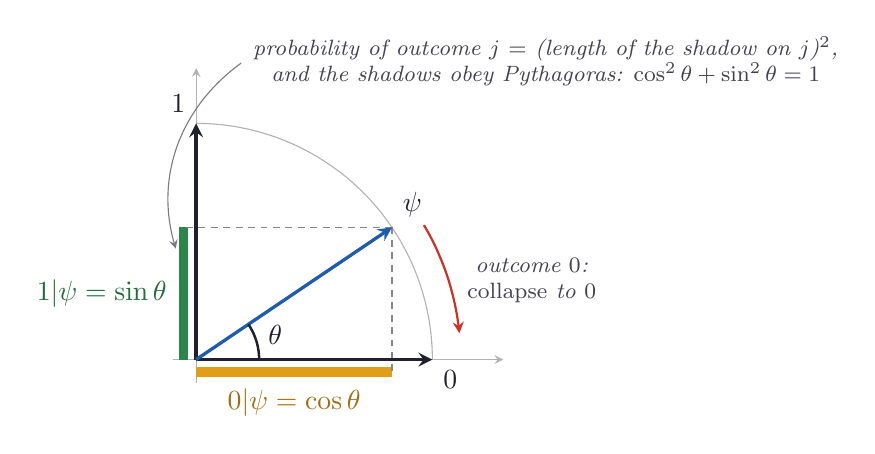
\begin{tikzpicture}[ink/.style={line width=0.9pt, ndInk}, faint/.style={line width=0.4pt, ndInk!35}, dashedink/.style={line width=0.5pt, ndInk!55, dash pattern=on 2.5pt off 2pt}, vec/.style={->, >=stealth, line width=1.2pt}, note/.style={font=\footnotesize\itshape, text=ndInk!85, align=center}, pointer/.style={->, >=stealth, line width=0.4pt, ndInk!60, shorten >=2pt, shorten <=1pt}, dot/.style={circle, fill=ndInk, inner sep=0pt, minimum size=3.4pt}, wash/.style={fill=ndSky, fill opacity=0.55}, every node/.style={text=ndInk}]
\definecolor{ndInk}{rgb}{0.13,0.13,0.18}
\definecolor{ndPaper}{rgb}{0.99,0.96,0.88}
\definecolor{ndSky}{rgb}{0.84,0.91,0.98}
\definecolor{ndRose}{rgb}{0.98,0.86,0.84}
\definecolor{ndBlue}{rgb}{0.13,0.36,0.66}
\definecolor{ndRed}{rgb}{0.78,0.20,0.16}
\definecolor{ndGold}{rgb}{0.88,0.62,0.10}
\definecolor{ndGreen}{rgb}{0.18,0.52,0.30}
\draw[faint] (3.000,0.000) -- (2.999,0.080) -- (2.996,0.160) -- (2.990,0.239) -- (2.983,0.319) -- (2.973,0.398) -- (2.962,0.477) -- (2.948,0.556) -- (2.932,0.634) -- (2.914,0.712) -- (2.894,0.789) -- (2.872,0.866) -- (2.848,0.942) -- (2.822,1.018) -- (2.794,1.092) -- (2.764,1.166) -- (2.732,1.240) -- (2.698,1.312) -- (2.662,1.383) -- (2.624,1.454) -- (2.585,1.523) -- (2.543,1.591) -- (2.500,1.658) -- (2.455,1.724) -- (2.408,1.789) -- (2.360,1.853) -- (2.310,1.915) -- (2.258,1.976) -- (2.204,2.035) -- (2.149,2.093) -- (2.093,2.149) -- (2.035,2.204) -- (1.976,2.258) -- (1.915,2.310) -- (1.853,2.360) -- (1.789,2.408) -- (1.724,2.455) -- (1.658,2.500) -- (1.591,2.543) -- (1.523,2.585) -- (1.454,2.624) -- (1.383,2.662) -- (1.312,2.698) -- (1.240,2.732) -- (1.166,2.764) -- (1.092,2.794) -- (1.018,2.822) -- (0.942,2.848) -- (0.866,2.872) -- (0.789,2.894) -- (0.712,2.914) -- (0.634,2.932) -- (0.556,2.948) -- (0.477,2.962) -- (0.398,2.973) -- (0.319,2.983) -- (0.239,2.990) -- (0.160,2.996) -- (0.080,2.999) -- (0.000,3.000);
\draw[faint, ->, >=stealth] (-0.3,0) -- (3.90,0);
\draw[faint, ->, >=stealth] (0,-0.3) -- (0,3.70);
\draw[line width=3.4pt, ndGold] (0,-0.160) -- (2.487,-0.160);
\draw[line width=3.4pt, ndGreen] (-0.160,0) -- (-0.160,1.678);
\draw[dashedink] (2.487,1.678) -- (2.487,-0.160);
\draw[dashedink] (2.487,1.678) -- (-0.160,1.678);
\draw[vec, ndInk] (0,0) -- (3.000,0) node[below right] {$\ket0$};
\draw[vec, ndInk] (0,0) -- (0,3.000) node[above left] {$\ket1$};
\draw[vec, ndBlue] (0,0) -- (2.487,1.678) node[above right] {$\ket\psi$};
\draw[ink] (0.800,0.000) -- (0.800,0.025) -- (0.798,0.050) -- (0.796,0.075) -- (0.794,0.100) -- (0.790,0.124) -- (0.786,0.149) -- (0.781,0.174) -- (0.775,0.198) -- (0.769,0.222) -- (0.761,0.246) -- (0.753,0.269) -- (0.744,0.293) -- (0.735,0.316) -- (0.725,0.339) -- (0.714,0.361) -- (0.702,0.383) -- (0.690,0.405) -- (0.677,0.426) -- (0.663,0.447);
\node at (1.004,0.307) {$\theta$};
\node[ndGold!70!black, below] at (1.244,-0.25) {$\braket{0|\psi}=\cos\theta$};
\node[ndGreen!80!black, left] at (-0.25,0.839) {$\braket{1|\psi}=\sin\theta$};
\draw[->, >=stealth, line width=0.8pt, ndRed] (2.893,1.708) -- (2.918,1.665) -- (2.943,1.621) -- (2.967,1.577) -- (2.990,1.533) -- (3.013,1.488) -- (3.035,1.443) -- (3.056,1.397) -- (3.076,1.351) -- (3.096,1.305) -- (3.115,1.259) -- (3.134,1.212) -- (3.152,1.165) -- (3.169,1.118) -- (3.185,1.070) -- (3.201,1.023) -- (3.216,0.975) -- (3.230,0.926) -- (3.243,0.878) -- (3.256,0.829) -- (3.268,0.781) -- (3.279,0.732) -- (3.290,0.683) -- (3.300,0.633) -- (3.309,0.584) -- (3.317,0.535) -- (3.325,0.485) -- (3.332,0.435) -- (3.338,0.385) -- (3.343,0.335);
\node[note, right] at (3.321,1.000) {outcome $0$:\\ \emph{collapse} to $\ket0$};
\node[note, anchor=south west] (m) at (0.6,3.35) {probability of outcome $j$ $=$ (length of the shadow on $\ket j$)$^2$,\\and the shadows obey Pythagoras: $\cos^2\theta+\sin^2\theta=1$};
\draw[pointer] (m.west) to[bend right=35] (-0.240,1.342);
\end{tikzpicture}
}
\caption{The Born rule as the squared length of a shadow: $\Prob(j)=\abs{\braket{j|\psi}}^2$, and after outcome $0$ the state collapses to $\ket0$. Generated by \texttt{code/ch02\_born.py}.}\label{fig:ch02:born}
\end{figure}}
\onp{\begin{center}\resizebox{!}{0.6\textheight}{% Generated by code/needham.py -- do not edit by hand.
\definecolor{qocA}{rgb}{0.00,0.45,0.70}
\definecolor{qocB}{rgb}{0.90,0.60,0.00}
\definecolor{qocC}{rgb}{0.00,0.62,0.45}
\definecolor{qocD}{rgb}{0.80,0.40,0.00}
\definecolor{qocE}{rgb}{0.80,0.60,0.70}
\definecolor{qocF}{rgb}{0.35,0.70,0.90}
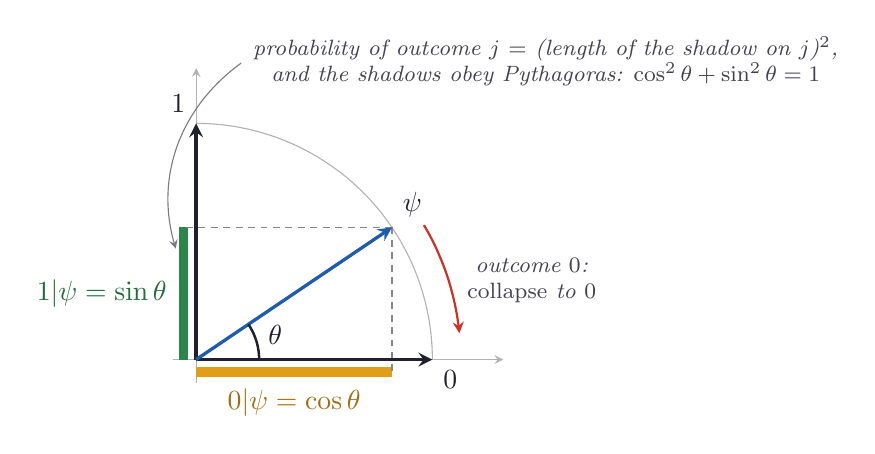
\begin{tikzpicture}[ink/.style={line width=0.9pt, ndInk}, faint/.style={line width=0.4pt, ndInk!35}, dashedink/.style={line width=0.5pt, ndInk!55, dash pattern=on 2.5pt off 2pt}, vec/.style={->, >=stealth, line width=1.2pt}, note/.style={font=\footnotesize\itshape, text=ndInk!85, align=center}, pointer/.style={->, >=stealth, line width=0.4pt, ndInk!60, shorten >=2pt, shorten <=1pt}, dot/.style={circle, fill=ndInk, inner sep=0pt, minimum size=3.4pt}, wash/.style={fill=ndSky, fill opacity=0.55}, every node/.style={text=ndInk}]
\definecolor{ndInk}{rgb}{0.13,0.13,0.18}
\definecolor{ndPaper}{rgb}{0.99,0.96,0.88}
\definecolor{ndSky}{rgb}{0.84,0.91,0.98}
\definecolor{ndRose}{rgb}{0.98,0.86,0.84}
\definecolor{ndBlue}{rgb}{0.13,0.36,0.66}
\definecolor{ndRed}{rgb}{0.78,0.20,0.16}
\definecolor{ndGold}{rgb}{0.88,0.62,0.10}
\definecolor{ndGreen}{rgb}{0.18,0.52,0.30}
\draw[faint] (3.000,0.000) -- (2.999,0.080) -- (2.996,0.160) -- (2.990,0.239) -- (2.983,0.319) -- (2.973,0.398) -- (2.962,0.477) -- (2.948,0.556) -- (2.932,0.634) -- (2.914,0.712) -- (2.894,0.789) -- (2.872,0.866) -- (2.848,0.942) -- (2.822,1.018) -- (2.794,1.092) -- (2.764,1.166) -- (2.732,1.240) -- (2.698,1.312) -- (2.662,1.383) -- (2.624,1.454) -- (2.585,1.523) -- (2.543,1.591) -- (2.500,1.658) -- (2.455,1.724) -- (2.408,1.789) -- (2.360,1.853) -- (2.310,1.915) -- (2.258,1.976) -- (2.204,2.035) -- (2.149,2.093) -- (2.093,2.149) -- (2.035,2.204) -- (1.976,2.258) -- (1.915,2.310) -- (1.853,2.360) -- (1.789,2.408) -- (1.724,2.455) -- (1.658,2.500) -- (1.591,2.543) -- (1.523,2.585) -- (1.454,2.624) -- (1.383,2.662) -- (1.312,2.698) -- (1.240,2.732) -- (1.166,2.764) -- (1.092,2.794) -- (1.018,2.822) -- (0.942,2.848) -- (0.866,2.872) -- (0.789,2.894) -- (0.712,2.914) -- (0.634,2.932) -- (0.556,2.948) -- (0.477,2.962) -- (0.398,2.973) -- (0.319,2.983) -- (0.239,2.990) -- (0.160,2.996) -- (0.080,2.999) -- (0.000,3.000);
\draw[faint, ->, >=stealth] (-0.3,0) -- (3.90,0);
\draw[faint, ->, >=stealth] (0,-0.3) -- (0,3.70);
\draw[line width=3.4pt, ndGold] (0,-0.160) -- (2.487,-0.160);
\draw[line width=3.4pt, ndGreen] (-0.160,0) -- (-0.160,1.678);
\draw[dashedink] (2.487,1.678) -- (2.487,-0.160);
\draw[dashedink] (2.487,1.678) -- (-0.160,1.678);
\draw[vec, ndInk] (0,0) -- (3.000,0) node[below right] {$\ket0$};
\draw[vec, ndInk] (0,0) -- (0,3.000) node[above left] {$\ket1$};
\draw[vec, ndBlue] (0,0) -- (2.487,1.678) node[above right] {$\ket\psi$};
\draw[ink] (0.800,0.000) -- (0.800,0.025) -- (0.798,0.050) -- (0.796,0.075) -- (0.794,0.100) -- (0.790,0.124) -- (0.786,0.149) -- (0.781,0.174) -- (0.775,0.198) -- (0.769,0.222) -- (0.761,0.246) -- (0.753,0.269) -- (0.744,0.293) -- (0.735,0.316) -- (0.725,0.339) -- (0.714,0.361) -- (0.702,0.383) -- (0.690,0.405) -- (0.677,0.426) -- (0.663,0.447);
\node at (1.004,0.307) {$\theta$};
\node[ndGold!70!black, below] at (1.244,-0.25) {$\braket{0|\psi}=\cos\theta$};
\node[ndGreen!80!black, left] at (-0.25,0.839) {$\braket{1|\psi}=\sin\theta$};
\draw[->, >=stealth, line width=0.8pt, ndRed] (2.893,1.708) -- (2.918,1.665) -- (2.943,1.621) -- (2.967,1.577) -- (2.990,1.533) -- (3.013,1.488) -- (3.035,1.443) -- (3.056,1.397) -- (3.076,1.351) -- (3.096,1.305) -- (3.115,1.259) -- (3.134,1.212) -- (3.152,1.165) -- (3.169,1.118) -- (3.185,1.070) -- (3.201,1.023) -- (3.216,0.975) -- (3.230,0.926) -- (3.243,0.878) -- (3.256,0.829) -- (3.268,0.781) -- (3.279,0.732) -- (3.290,0.683) -- (3.300,0.633) -- (3.309,0.584) -- (3.317,0.535) -- (3.325,0.485) -- (3.332,0.435) -- (3.338,0.385) -- (3.343,0.335);
\node[note, right] at (3.321,1.000) {outcome $0$:\\ \emph{collapse} to $\ket0$};
\node[note, anchor=south west] (m) at (0.6,3.35) {probability of outcome $j$ $=$ (length of the shadow on $\ket j$)$^2$,\\and the shadows obey Pythagoras: $\cos^2\theta+\sin^2\theta=1$};
\draw[pointer] (m.west) to[bend right=35] (-0.240,1.342);
\end{tikzpicture}
}\end{center}}
\end{frame}

\begin{frame}\ft{An example: measurements disturb}
\ona{Here is the second classical property failing. Prepare a qubit in $\ket0$ and measure $\sigz$: the outcome is $+1$ with certainty, and it stays $+1$ however often we repeat. Now measure $\sigx$ instead. Its eigenvectors are $\ket\pm$, and}
\onp{Start in $\ket0$. Measure $\sigz$: $+1$, again and again. Now measure $\sigx$ (eigenvectors $\ket\pm$):}
\[
\Prob(\pm1)=\abs{\braket{\pm|0}}^2=\tfrac12 .
\]
\ona{Say we obtain $+1$; the state is now $\ket+$. If we return to $\sigz$, the outcomes $\pm1$ are equally likely, $\abs{\braket{0|+}}^2=\abs{\braket{1|+}}^2=\tfrac12$: the intermediate measurement of $\sigx$ has erased what we knew. For the die, this would mean that looking at the side of the die changes the number on top. The reason is that $\sigz$ and $\sigx$ do not commute, $\comm{\sigz}{\sigx}=2\imath\sigy\ne0$, so they have no common eigenbasis. Quantitatively, for any state and observables, the standard deviations $\Delta A=\big(\braket{A^2}_\psi-\braket{A}_\psi^2\big)^{1/2}$ obey the \emph{uncertainty relation}}
\onp{Get $+1$: the state is $\ket+$. Measure $\sigz$ again: $\pm1$ with probability $\tfrac12$ each. The $\sigx$ measurement \alert{erased} the $\sigz$ information, because $\comm{\sigz}{\sigx}=2\imath\sigy\ne0$. In general:}
\begin{equation}\label{eq:ch02:uncertainty}
\Delta A\,\Delta B\ \ge\ \tfrac12\,\abs{\braket{\psi|\comm AB|\psi}},
\end{equation}
\ona{due to Heisenberg and Robertson (Exercise~\ref{exe:ch02:uncertainty}). Only commuting observables can be measured together without disturbing each other.}
\end{frame}

\begin{frame}\ft{Global and relative phases}
\ona{Multiplying a state by a complex number of modulus one, $\ket\psi\mapsto\ee^{\imath\gamma}\ket\psi$, changes no probability: $\abs{\braket{a_j|\ee^{\imath\gamma}\psi}}^2=\abs{\braket{a_j|\psi}}^2$. Such a \emph{global phase} is unobservable, and states that differ only by a global phase are the same physical state. A \emph{relative} phase between components is observable, however. The states $\ket+$ and $\ket-$ differ only by the sign of the $\ket1$ component and give the same statistics for $\sigz$, yet a measurement of $\sigx$ tells them apart with certainty. More generally, two states can be distinguished with certainty by a single measurement if and only if they are orthogonal; non-orthogonal states always have some probability of producing the same outcome.}
\onp{\begin{itemize}\setlength\itemsep{0.5em}
    \item \alert{Global phase} $\ee^{\imath\gamma}\ket\psi$: same probabilities for every measurement, same physical state.
    \item \alert{Relative phase} matters: $\ket\pm=\tfrac1{\sqrt2}(\ket0\pm\ket1)$ look alike to $\sigz$, but $\sigx$ tells them apart.
    \item Two states are perfectly distinguishable $\Leftrightarrow$ they are orthogonal.
\end{itemize}}
\end{frame}

\begin{frame}\ft{Composite systems and entanglement}
\ona{Two systems with Hilbert spaces $\Hil_A\cong\C^{N_A}$ and $\Hil_B\cong\C^{N_B}$ together form a system with the \emph{tensor product} space $\Hil_A\otimes\Hil_B\cong\C^{N_AN_B}$. Concretely, the tensor product of vectors and matrices is the \emph{Kronecker product},}
\onp{Two systems together: the \alert{tensor product} $\Hil_A\otimes\Hil_B\cong\C^{N_AN_B}$, computed with the Kronecker product}
\[
A\otimes B=\begin{pmatrix}a_{11}B&\cdots&a_{1n}B\\ \vdots&&\vdots\\ a_{n1}B&\cdots&a_{nn}B\end{pmatrix},\qquad
\ket0\otimes\ket1=\begin{pmatrix}1\\0\end{pmatrix}\otimes\begin{pmatrix}0\\1\end{pmatrix}=\begin{pmatrix}0\\1\\0\\0\end{pmatrix},
\]
\ona{and we abbreviate $\ket j\otimes\ket k=\ket{jk}$. Dimensions multiply, so $q$ qubits live in $\C^{2^q}$; this exponential growth is what makes quantum systems hard to simulate. Operators act factor by factor, $(A\otimes B)(\ket a\otimes\ket b)=A\ket a\otimes B\ket b$, and $(A\otimes B)(C\otimes D)=AC\otimes BD$. For qubits, tensor products of Pauli matrices such as $\sigz\otimes\sigz$ or $\sigx\otimes\Id$ are called \emph{Pauli strings}. A state of the form $\ket a\otimes\ket b$ is a \emph{product state}. Most states are not: the Bell state}
\onp{$\ket j\otimes\ket k=\ket{jk}$; $q$ qubits: $\C^{2^q}$. $(A\otimes B)(C\otimes D)=AC\otimes BD$; \alert{Pauli strings} $\sigz\otimes\sigz$, $\sigx\otimes\Id,\dots$ Most states are not products $\ket a\otimes\ket b$:}
\begin{equation}\label{eq:ch02:bell}
\ket{\Phi^+}=\tfrac1{\sqrt2}\big(\ket{00}+\ket{11}\big)
\end{equation}
\ona{cannot be written as $(a_0\ket0+a_1\ket1)\otimes(b_0\ket0+b_1\ket1)$, since this would need $a_0b_1=0$ although $a_0b_0\ne0$ and $a_1b_1\ne0$. Such states are \emph{entangled}. Measuring $\sigz$ on either qubit of $\ket{\Phi^+}$ gives $\pm1$ at random, but the two outcomes always agree.}
\onp{is \alert{entangled}: each qubit alone is random, but the two $\sigz$ outcomes always agree.}
\end{frame}

\begin{frame}\ft{Evolution is unitary; the Hamiltonian}
\ona{How does a state change in time? Write $\ket{\psi(t)}=U(t)\ket{\psi(0)}$ for a linear map $U(t)$. Physics requires that probabilities stay normalised and that perfectly distinguishable (orthogonal) states stay distinguishable. Applied to an orthonormal basis, this means $\braket{a_j|U(t)^\dagger U(t)|a_k}=\delta_{jk}$, i.e.\ $U(t)^\dagger U(t)=\Id$: \emph{time evolution is unitary}. Now consider a very short time $\delta t$ and write $U(\delta t)=\Id-\imath H\,\delta t+O(\delta t^2)$ for some matrix $H$. Unitarity gives}
\onp{Evolution $\ket{\psi(t)}=U(t)\ket{\psi(0)}$ must keep normalisation and orthogonality: $U^\dagger U=\Id$, \alert{unitary}. For a short step, $U(\delta t)=\Id-\imath H\delta t+O(\delta t^2)$, and}
\[
\Id=U(\delta t)^\dagger U(\delta t)=\Id+\imath\,\delta t\,(H^\dagger-H)+O(\delta t^2),
\]
\ona{so $H^\dagger=H$. This Hermitian matrix is the \emph{Hamiltonian}, the observable of the system's energy. Letting $\delta t\to0$ in $\ket{\psi(t+\delta t)}=U(\delta t)\ket{\psi(t)}$ gives the \emph{Schr\"odinger equation} $\imath\,\tfrac{\mathrm d}{\mathrm dt}\ket{\psi(t)}=H\ket{\psi(t)}$. Properly, the left-hand side carries Planck's constant $\hbar\approx1.055\times10^{-34}\,\mathrm{J\,s}$; we measure energies in units of angular frequency, which sets $\hbar=1$. The eigenvectors of $H$, $H\ket{E_j}=E_j\ket{E_j}$, are the \emph{energy eigenstates}; they merely acquire a phase in time, $\ket{E_j}\mapsto\ee^{-\imath E_jt}\ket{E_j}$, and are therefore called stationary. Evolution of the state is deterministic; randomness enters only through measurement. Section~\ref{sec:ch02:schrodinger} treats time-dependent Hamiltonians.}
\ona{\endgraf\medskip\noindent\emph{Two theorems behind the argument.} The derivation assumed that $U(t)$ is linear and differentiable; both assumptions can be derived. \emph{Wigner's theorem} states that every bijection of the pure states (unit vectors up to phase) that preserves all transition probabilities $\abs{\braket{\varphi|\psi}}^2$ is induced by an operator that is either unitary or \emph{antiunitary} (conjugate-linear and inner-product preserving up to complex conjugation), unique up to a phase. Evolution depends continuously on $t$ and starts at the identity, and $U(t)=U(t/2)^2$ is the square of a unitary or of an antiunitary, which is unitary in both cases: time evolution is linear and unitary. \emph{Stone's theorem} states that every continuous one-parameter group of unitaries, $U(s+t)=U(s)U(t)$, is of the form $U(t)=\ee^{-\imath Ht}$ for a unique self-adjoint $H$. In finite dimensions $H$ is a Hermitian matrix and $U$ is automatically smooth; in infinite dimensions $H$ may be unbounded and defined only on a dense subspace, which is the situation of the harmonic oscillator in Section~\ref{sec:ch02:examples}.}
\onp{so $H^\dagger=H$: the \alert{Hamiltonian} (energy). In the limit, the \alert{Schr\"odinger equation} $\imath\frac{\mathrm d}{\mathrm dt}\ket\psi=H\ket\psi$ (units with $\hbar=1$). Energy eigenstates only pick up phases $\ee^{-\imath E_jt}$.}
\end{frame}

\begin{frame}\ft{The matrix exponential}
\ona{For a constant Hamiltonian the solution of the Schr\"odinger equation is $\ket{\psi(t)}=\ee^{-\imath Ht}\ket{\psi(0)}$, where the exponential of a square matrix is defined by the same power series as for numbers:}
\onp{For constant $H$: $\ket{\psi(t)}=\ee^{-\imath Ht}\ket{\psi(0)}$, with}
\begin{equation}\label{eq:ch02:expm}
\ee^{A}=\sum_{k=0}^\infty\frac{A^k}{k!}=\Id+A+\tfrac12A^2+\dots,\qquad \dd{t}\ee^{tA}=A\,\ee^{tA}=\ee^{tA}A .
\end{equation}
\ona{The series converges for every matrix. Three rules are worth remembering. First, $\ee^{sA}\ee^{tA}=\ee^{(s+t)A}$, and more generally $\ee^{A}\ee^{B}=\ee^{A+B}$ whenever $A$ and $B$ commute. For non-commuting matrices the identity fails in general (it can hold by accident, e.g.\ for $A=\operatorname{diag}(0,2\pi\imath)$ and $B=\big(\begin{smallmatrix}0&0\\1&2\pi\imath\end{smallmatrix}\big)$, where both sides equal $\Id$); how it fails is the subject of Section~\ref{sec:ch02:lie}. Second, if $H=\sum_jE_j\ket{E_j}\bra{E_j}$, then $\ee^{-\imath Ht}=\sum_j\ee^{-\imath E_jt}\ket{E_j}\bra{E_j}$: exponentiate the eigenvalues. Third, if $\sigma^2=\Id$, as for every Pauli matrix, the even and odd terms of the series separate into a cosine and a sine,}
\onp{\begin{itemize}
    \item $\ee^{sA}\ee^{tA}=\ee^{(s+t)A}$; $\ee^A\ee^B=\ee^{A+B}$ if $\comm AB=0$, but not in general.
    \item $H=\sum_jE_j\ket{E_j}\bra{E_j}$ $\Rightarrow$ $\ee^{-\imath Ht}=\sum_j\ee^{-\imath E_jt}\ket{E_j}\bra{E_j}$.
    \item $\sigma^2=\Id$ (every Pauli matrix):
\end{itemize}}
\begin{equation}\label{eq:ch02:pauli-exp}
\ee^{-\imath\theta\sigma/2}=\cos\tfrac\theta2\,\Id-\imath\sin\tfrac\theta2\,\sigma .
\end{equation}
\ona{For example, $H=\tfrac12\sigx$ acting for time $\theta=\pi$ sends $\ket0$ to $\ee^{-\imath\pi\sigx/2}\ket0=-\imath\ket1$: it flips the qubit, up to a global phase. This is the $\pi$-pulse of \Chap~\ref{C.Motivation}.}
\onp{E.g.\ $\ee^{-\imath\pi\sigx/2}\ket0=-\imath\ket1$: a \alert{$\pi$-pulse} flips the qubit.}
\end{frame}

\begin{frame}[allowframebreaks]\ft{Exercises}
\begin{exe}\label{exe:ch02:normalise}
Normalise $\ket{01}-\ket{10}$ and $\ket{000}+\ket{111}$, and write them as column vectors in $\C^4$ and $\C^8$.
\end{exe}
\begin{exe}\label{exe:ch02:pauli}
Show that $\sigx,\sigy,\sigz$ are Hermitian and unitary, compute all their commutators and anticommutators, and verify \eqref{eq:ch02:pauli-comm}. Find their eigenvalues and eigenvectors.
\end{exe}
\begin{exe}
Show that eigenvectors of a Hermitian matrix with different eigenvalues are orthogonal.
\end{exe}
\begin{exe}
For the normalised state $\tfrac1{\sqrt6}\big((1-\imath)\ket0+2\imath\ket1\big)$, compute the probabilities of the outcomes $\pm1$ for measurements of $\sigz$ and of $\sigx$, and the expectation values $\braket{\sigz}$ and $\braket{\sigx}$.
\end{exe}
\begin{exe}
Compute $\braket{\sigz\otimes\sigz}$ in the normalised state $\tfrac1{\sqrt2}(\ket{01}-\ket{10})$.
\end{exe}
\begin{exe}\label{exe:ch02:uncertainty}
Prove \eqref{eq:ch02:uncertainty}. Hint: replace $A$ by $A-\braket{A}_\psi\Id$ and $B$ likewise, and apply the Cauchy--Schwarz inequality $\abs{\braket{u|v}}\le\norm u\,\norm v$ to $\ket u=A\ket\psi$, $\ket v=B\ket\psi$, keeping only the imaginary part of $\braket{u|v}$.
\end{exe}
\begin{exe}
Compute $\ee^{-\imath\theta\sigz/2}$ and $\ee^{-\imath\theta\sigy/2}$ as $2\times2$ matrices, and apply them to $\ket0$ and to $\ket+$.
\end{exe}
\begin{exe}
Alice and Bob study a system with $\Hil=\C^3$. Alice measures an observable with outcomes red, green and blue; Bob measures one with outcomes sweet, tangy and umami. If Alice finds red, Bob then finds sweet, tangy and umami with probabilities $0$, $p$ and $1-p$. If Alice finds green, Bob's probabilities are $q$, $0$ and $1-q$. Which values of $p$ and $q$ are possible? What are Bob's probabilities if Alice finds blue?
\end{exe}
\end{frame}

\begin{frame}\ft{The postulates, summarised}\label{frame:ch02:postulates}
\ona{We summarise this section in the four postulates of quantum mechanics.}
\begin{itemize}\setlength\itemsep{0.4em}
    \item \textbf{States.} A system is associated with a Hilbert space $\Hil\cong\C^N$. Pure states are unit vectors $\ket\psi\in\Hil$, up to a global phase.
    \item \textbf{Observables and measurement.} Observables are Hermitian operators $M\in\Herm[\Hil]$. Measuring $M=\sum_\lambda \lambda\,\Pi_\lambda$ yields outcome $\lambda$ with probability $\Prob(\lambda)=\braket{\psi|\Pi_\lambda|\psi}$ and leaves the system in $\Pi_\lambda\ket\psi/\norm{\Pi_\lambda\ket\psi}$. The expectation is $\braket{\psi|M|\psi}$.
    \item \textbf{Composite systems.} $\Hil_{AB}=\Hil_A\otimes\Hil_B$.
    \item \textbf{Evolution.} Closed-system evolution is unitary, $\ket{\psi(t)}=U(t)\ket{\psi(0)}$ with $U(t)\in\Un[N]$, generated by a Hamiltonian through the Schr\"odinger equation.
\end{itemize}
\ona{Two generalisations follow later in this \chap{}: density operators (Section~\ref{sec:ch02:density}) describe states that are only partly known, and POVMs (Section~\ref{sec:ch02:povm}) describe realistic measurements.}
\onp{Later: density operators (partly known states) and POVMs (realistic measurements).}
\end{frame}

\section{Lie groups and Lie algebras}\label{sec:ch02:lie}

\begin{frame}\ft{Groups}
\ona{The unitary matrices that describe evolution can be multiplied (one evolution followed by another) and inverted (undo an evolution), and they include the identity (do nothing). Structures of this kind are called groups.}
\begin{defn}[Group]\label{def:ch02:group}
A group is a set $G$ with a multiplication $G\times G\to G$, $(g,h)\mapsto gh$, that is associative, $(gh)k=g(hk)$, has an identity element $e$ with $eg=ge=g$, and in which every $g$ has an inverse $g^{-1}$ with $gg^{-1}=g^{-1}g=e$.
\end{defn}
\ona{The multiplication need not be commutative: in general $gh\ne hg$. Examples:}
\onp{In general $gh\ne hg$. Examples:}
\begin{itemize}\setlength\itemsep{0.2em}
    \item the complex numbers of modulus one, $\Un[1]=\{\ee^{\imath\varphi}\}$, under multiplication: the unit circle;
    \item the rotations of the plane, $\mathrm{SO}(2)$, and of space, $\mathrm{SO}(3)$ (the latter is not commutative);
    \item the invertible $N\times N$ matrices; the unitary matrices $\Un[N]$; and $\SU[N]=\{U\in\Un[N]:\det U=1\}$.
\end{itemize}
\ona{The unitary matrices form a group because $(UV)^\dagger UV=V^\dagger U^\dagger UV=\Id$ and $U^{-1}=U^\dagger$.}
\ona{All these groups are also smooth ``curved spaces'' (manifolds): $\Un[1]$ is a circle, $\SU[2]$ turns out to be the three-dimensional sphere in $\R^4$, and near each of their points they look like a piece of $\R^d$. Groups of this kind, in which one can differentiate, are called \emph{Lie groups}, after Sophus Lie. Differentiation is what we need: evolution in time traces out a curve $t\mapsto U(t)$ in the group.}
\onp{All are \alert{Lie groups}: smooth curved spaces ($\Un[1]$ is a circle) in which we can differentiate. Evolution traces a \alert{curve} $t\mapsto U(t)$ in the group.}
\end{frame}

\begin{frame}\ft{One-parameter groups and their generators}
\ona{The simplest curves in a matrix group are those of the form $t\mapsto\ee^{tX}$ for a fixed matrix $X$. By \eqref{eq:ch02:expm}, they satisfy $\ee^{sX}\ee^{tX}=\ee^{(s+t)X}$ and $\ee^{0X}=\Id$, so they are \emph{one-parameter groups}, and their velocity at $t=0$ is $X$, the \emph{generator}. Figure~\ref{fig:ch02:rotation} shows the rotations of the plane: for $J=\big(\begin{smallmatrix}0&-1\\1&0\end{smallmatrix}\big)$ we have $J^2=-\Id$, and the power series gives $\ee^{tJ}=\cos t\,\Id+\sin t\,J$, the rotation by the angle $t$.}
\onp{$t\mapsto\ee^{tX}$: a \alert{one-parameter group}, $\ee^{sX}\ee^{tX}=\ee^{(s+t)X}$, with velocity $X$ at $t=0$ (the \alert{generator}).}
\ona{\begin{figure}[h]\centering
\resizebox{0.85\linewidth}{!}{% Generated by code/needham.py -- do not edit by hand.
\definecolor{qocA}{rgb}{0.00,0.45,0.70}
\definecolor{qocB}{rgb}{0.90,0.60,0.00}
\definecolor{qocC}{rgb}{0.00,0.62,0.45}
\definecolor{qocD}{rgb}{0.80,0.40,0.00}
\definecolor{qocE}{rgb}{0.80,0.60,0.70}
\definecolor{qocF}{rgb}{0.35,0.70,0.90}
\begin{tikzpicture}[ink/.style={line width=0.9pt, ndInk}, faint/.style={line width=0.4pt, ndInk!35}, dashedink/.style={line width=0.5pt, ndInk!55, dash pattern=on 2.5pt off 2pt}, vec/.style={->, >=stealth, line width=1.2pt}, note/.style={font=\footnotesize\itshape, text=ndInk!85, align=center}, pointer/.style={->, >=stealth, line width=0.4pt, ndInk!60, shorten >=2pt, shorten <=1pt}, dot/.style={circle, fill=ndInk, inner sep=0pt, minimum size=3.4pt}, wash/.style={fill=ndSky, fill opacity=0.55}, every node/.style={text=ndInk}]
\definecolor{ndInk}{rgb}{0.13,0.13,0.18}
\definecolor{ndPaper}{rgb}{0.99,0.96,0.88}
\definecolor{ndSky}{rgb}{0.84,0.91,0.98}
\definecolor{ndRose}{rgb}{0.98,0.86,0.84}
\definecolor{ndBlue}{rgb}{0.13,0.36,0.66}
\definecolor{ndRed}{rgb}{0.78,0.20,0.16}
\definecolor{ndGold}{rgb}{0.88,0.62,0.10}
\definecolor{ndGreen}{rgb}{0.18,0.52,0.30}
\fill[ndSky, fill opacity=0.35] (0,0) circle (2.600);
\draw[faint] (0,0) circle (2.600);
\draw[faint, ->, >=stealth] (-3.00,0) -- (3.10,0) node[above] {$x_1$};
\draw[faint, ->, >=stealth] (0,-3.00) -- (0,3.20) node[left] {$x_2$};
\draw[line width=1.8pt, ndBlue] (2.600,0.000) -- (2.600,0.046) -- (2.598,0.092) -- (2.596,0.138) -- (2.594,0.183) -- (2.590,0.229) -- (2.585,0.275) -- (2.580,0.320) -- (2.574,0.366) -- (2.567,0.411) -- (2.560,0.456) -- (2.551,0.502) -- (2.542,0.546) -- (2.532,0.591) -- (2.521,0.636) -- (2.509,0.680) -- (2.497,0.724) -- (2.484,0.768) -- (2.470,0.812) -- (2.455,0.856) -- (2.440,0.899) -- (2.423,0.942) -- (2.407,0.984) -- (2.389,1.027) -- (2.370,1.069) -- (2.351,1.110) -- (2.331,1.152) -- (2.310,1.192) -- (2.289,1.233) -- (2.267,1.273) -- (2.244,1.313) -- (2.221,1.352) -- (2.196,1.391) -- (2.171,1.430) -- (2.146,1.468) -- (2.120,1.506) -- (2.093,1.543) -- (2.065,1.580) -- (2.037,1.616) -- (2.008,1.651) -- (1.979,1.687) -- (1.949,1.721) -- (1.918,1.755) -- (1.887,1.789) -- (1.855,1.822) -- (1.822,1.854) -- (1.789,1.886) -- (1.756,1.918) -- (1.722,1.948) -- (1.687,1.978) -- (1.652,2.008) -- (1.616,2.037) -- (1.580,2.065) -- (1.543,2.092) -- (1.506,2.119) -- (1.469,2.146) -- (1.430,2.171) -- (1.392,2.196) -- (1.353,2.220) -- (1.314,2.244) -- (1.274,2.267) -- (1.234,2.289) -- (1.193,2.310) -- (1.152,2.331) -- (1.111,2.351) -- (1.069,2.370) -- (1.027,2.389) -- (0.985,2.406) -- (0.942,2.423) -- (0.899,2.440) -- (0.856,2.455) -- (0.813,2.470) -- (0.769,2.484) -- (0.725,2.497) -- (0.681,2.509) -- (0.636,2.521) -- (0.592,2.532) -- (0.547,2.542) -- (0.502,2.551) -- (0.457,2.560) -- (0.412,2.567) -- (0.366,2.574) -- (0.321,2.580) -- (0.275,2.585) -- (0.230,2.590) -- (0.184,2.593) -- (0.138,2.596) -- (0.092,2.598) -- (0.046,2.600) -- (0.001,2.600) -- (-0.045,2.600) -- (-0.091,2.598) -- (-0.137,2.596) -- (-0.183,2.594) -- (-0.229,2.590) -- (-0.274,2.585) -- (-0.320,2.580) -- (-0.365,2.574) -- (-0.411,2.567) -- (-0.456,2.560) -- (-0.501,2.551) -- (-0.546,2.542) -- (-0.591,2.532) -- (-0.635,2.521) -- (-0.680,2.510) -- (-0.724,2.497) -- (-0.768,2.484) -- (-0.812,2.470) -- (-0.855,2.455) -- (-0.898,2.440) -- (-0.941,2.424) -- (-0.984,2.407) -- (-1.026,2.389) -- (-1.068,2.370) -- (-1.110,2.351) -- (-1.151,2.331) -- (-1.192,2.311) -- (-1.233,2.289) -- (-1.273,2.267) -- (-1.313,2.244);
\fill[ndBlue] (2.395,1.012) circle (1.6pt);
\fill[ndBlue] (1.811,1.865) circle (1.6pt);
\fill[ndBlue] (0.942,2.423) circle (1.6pt);
\fill[ndBlue] (-0.076,2.599) circle (1.6pt);
\fill[ndBlue] (-1.082,2.364) circle (1.6pt);
\draw[vec, ndInk] (0,0) -- (-1.313,2.244) node[midway, below left] {$\ee^{tJ}x$};
\draw[vec, ndRed] (-1.313,2.244) -- (-2.435,1.588) node[left, text=ndRed] {$J\,\ee^{tJ}x$};
\draw[ink, line width=0.5pt] (-1.186,2.029) -- (-1.402,1.902) -- (-1.528,2.118);
\draw[vec, ndInk] (0,0) -- (2.600,0.000) node[below left] {$x$};
\draw[vec, ndRed] (2.600,0.000) -- (2.600,1.300) node[right, text=ndRed] {$Jx$};
\draw[ink, line width=0.5pt] (0.600,0.000) -- (0.599,0.032) -- (0.597,0.064) -- (0.592,0.097) -- (0.586,0.128) -- (0.578,0.160) -- (0.569,0.190) -- (0.558,0.221) -- (0.545,0.251) -- (0.531,0.280) -- (0.515,0.308) -- (0.498,0.335) -- (0.479,0.361) -- (0.459,0.387) -- (0.437,0.411) -- (0.415,0.434) -- (0.391,0.455) -- (0.366,0.476) -- (0.340,0.495) -- (0.312,0.512) -- (0.284,0.528) -- (0.256,0.543) -- (0.226,0.556) -- (0.196,0.567) -- (0.165,0.577) -- (0.134,0.585) -- (0.102,0.591) -- (0.070,0.596) -- (0.038,0.599) -- (0.006,0.600) -- (-0.027,0.599) -- (-0.059,0.597) -- (-0.091,0.593) -- (-0.123,0.587) -- (-0.154,0.580) -- (-0.185,0.571) -- (-0.216,0.560) -- (-0.245,0.547) -- (-0.275,0.533) -- (-0.303,0.518);
\node at (0.423,0.737) {$t$};
\node[note, anchor=west] (a) at (3.90,2.2) {$J=\begin{pmatrix}0&-1\\1&0\end{pmatrix}$, \ $\ee^{tJ}=\begin{pmatrix}\cos t&-\sin t\\ \sin t&\cos t\end{pmatrix}$:\\the exponential of $J$ is a rotation};
\node[note, anchor=west] (b) at (3.90,0.2) {the velocity $J\,\ee^{tJ}x$ is always\\perpendicular to the position:\\ the curve stays on the circle};
\draw[pointer] (b.west) to[bend right=15] (2.680,0.900);
\node[note, anchor=west] (c) at (3.90,-1.8) {dots: equal steps of $t$,\\since $\ee^{sJ}\ee^{tJ}=\ee^{(s+t)J}$};
\draw[pointer] (c.west) to[bend right=10] (2.395,1.012);
\end{tikzpicture}
}
\caption{The generator $J$ of the rotations of the plane. The curve $t\mapsto\ee^{tJ}x$ (blue) stays on the circle because its velocity $J\,\ee^{tJ}x$ (red) is perpendicular to the position. Generated by \texttt{code/ch02\_rotation.py}.}\label{fig:ch02:rotation}
\end{figure}}
\onp{\begin{center}\resizebox{!}{0.5\textheight}{% Generated by code/needham.py -- do not edit by hand.
\definecolor{qocA}{rgb}{0.00,0.45,0.70}
\definecolor{qocB}{rgb}{0.90,0.60,0.00}
\definecolor{qocC}{rgb}{0.00,0.62,0.45}
\definecolor{qocD}{rgb}{0.80,0.40,0.00}
\definecolor{qocE}{rgb}{0.80,0.60,0.70}
\definecolor{qocF}{rgb}{0.35,0.70,0.90}
\begin{tikzpicture}[ink/.style={line width=0.9pt, ndInk}, faint/.style={line width=0.4pt, ndInk!35}, dashedink/.style={line width=0.5pt, ndInk!55, dash pattern=on 2.5pt off 2pt}, vec/.style={->, >=stealth, line width=1.2pt}, note/.style={font=\footnotesize\itshape, text=ndInk!85, align=center}, pointer/.style={->, >=stealth, line width=0.4pt, ndInk!60, shorten >=2pt, shorten <=1pt}, dot/.style={circle, fill=ndInk, inner sep=0pt, minimum size=3.4pt}, wash/.style={fill=ndSky, fill opacity=0.55}, every node/.style={text=ndInk}]
\definecolor{ndInk}{rgb}{0.13,0.13,0.18}
\definecolor{ndPaper}{rgb}{0.99,0.96,0.88}
\definecolor{ndSky}{rgb}{0.84,0.91,0.98}
\definecolor{ndRose}{rgb}{0.98,0.86,0.84}
\definecolor{ndBlue}{rgb}{0.13,0.36,0.66}
\definecolor{ndRed}{rgb}{0.78,0.20,0.16}
\definecolor{ndGold}{rgb}{0.88,0.62,0.10}
\definecolor{ndGreen}{rgb}{0.18,0.52,0.30}
\fill[ndSky, fill opacity=0.35] (0,0) circle (2.600);
\draw[faint] (0,0) circle (2.600);
\draw[faint, ->, >=stealth] (-3.00,0) -- (3.10,0) node[above] {$x_1$};
\draw[faint, ->, >=stealth] (0,-3.00) -- (0,3.20) node[left] {$x_2$};
\draw[line width=1.8pt, ndBlue] (2.600,0.000) -- (2.600,0.046) -- (2.598,0.092) -- (2.596,0.138) -- (2.594,0.183) -- (2.590,0.229) -- (2.585,0.275) -- (2.580,0.320) -- (2.574,0.366) -- (2.567,0.411) -- (2.560,0.456) -- (2.551,0.502) -- (2.542,0.546) -- (2.532,0.591) -- (2.521,0.636) -- (2.509,0.680) -- (2.497,0.724) -- (2.484,0.768) -- (2.470,0.812) -- (2.455,0.856) -- (2.440,0.899) -- (2.423,0.942) -- (2.407,0.984) -- (2.389,1.027) -- (2.370,1.069) -- (2.351,1.110) -- (2.331,1.152) -- (2.310,1.192) -- (2.289,1.233) -- (2.267,1.273) -- (2.244,1.313) -- (2.221,1.352) -- (2.196,1.391) -- (2.171,1.430) -- (2.146,1.468) -- (2.120,1.506) -- (2.093,1.543) -- (2.065,1.580) -- (2.037,1.616) -- (2.008,1.651) -- (1.979,1.687) -- (1.949,1.721) -- (1.918,1.755) -- (1.887,1.789) -- (1.855,1.822) -- (1.822,1.854) -- (1.789,1.886) -- (1.756,1.918) -- (1.722,1.948) -- (1.687,1.978) -- (1.652,2.008) -- (1.616,2.037) -- (1.580,2.065) -- (1.543,2.092) -- (1.506,2.119) -- (1.469,2.146) -- (1.430,2.171) -- (1.392,2.196) -- (1.353,2.220) -- (1.314,2.244) -- (1.274,2.267) -- (1.234,2.289) -- (1.193,2.310) -- (1.152,2.331) -- (1.111,2.351) -- (1.069,2.370) -- (1.027,2.389) -- (0.985,2.406) -- (0.942,2.423) -- (0.899,2.440) -- (0.856,2.455) -- (0.813,2.470) -- (0.769,2.484) -- (0.725,2.497) -- (0.681,2.509) -- (0.636,2.521) -- (0.592,2.532) -- (0.547,2.542) -- (0.502,2.551) -- (0.457,2.560) -- (0.412,2.567) -- (0.366,2.574) -- (0.321,2.580) -- (0.275,2.585) -- (0.230,2.590) -- (0.184,2.593) -- (0.138,2.596) -- (0.092,2.598) -- (0.046,2.600) -- (0.001,2.600) -- (-0.045,2.600) -- (-0.091,2.598) -- (-0.137,2.596) -- (-0.183,2.594) -- (-0.229,2.590) -- (-0.274,2.585) -- (-0.320,2.580) -- (-0.365,2.574) -- (-0.411,2.567) -- (-0.456,2.560) -- (-0.501,2.551) -- (-0.546,2.542) -- (-0.591,2.532) -- (-0.635,2.521) -- (-0.680,2.510) -- (-0.724,2.497) -- (-0.768,2.484) -- (-0.812,2.470) -- (-0.855,2.455) -- (-0.898,2.440) -- (-0.941,2.424) -- (-0.984,2.407) -- (-1.026,2.389) -- (-1.068,2.370) -- (-1.110,2.351) -- (-1.151,2.331) -- (-1.192,2.311) -- (-1.233,2.289) -- (-1.273,2.267) -- (-1.313,2.244);
\fill[ndBlue] (2.395,1.012) circle (1.6pt);
\fill[ndBlue] (1.811,1.865) circle (1.6pt);
\fill[ndBlue] (0.942,2.423) circle (1.6pt);
\fill[ndBlue] (-0.076,2.599) circle (1.6pt);
\fill[ndBlue] (-1.082,2.364) circle (1.6pt);
\draw[vec, ndInk] (0,0) -- (-1.313,2.244) node[midway, below left] {$\ee^{tJ}x$};
\draw[vec, ndRed] (-1.313,2.244) -- (-2.435,1.588) node[left, text=ndRed] {$J\,\ee^{tJ}x$};
\draw[ink, line width=0.5pt] (-1.186,2.029) -- (-1.402,1.902) -- (-1.528,2.118);
\draw[vec, ndInk] (0,0) -- (2.600,0.000) node[below left] {$x$};
\draw[vec, ndRed] (2.600,0.000) -- (2.600,1.300) node[right, text=ndRed] {$Jx$};
\draw[ink, line width=0.5pt] (0.600,0.000) -- (0.599,0.032) -- (0.597,0.064) -- (0.592,0.097) -- (0.586,0.128) -- (0.578,0.160) -- (0.569,0.190) -- (0.558,0.221) -- (0.545,0.251) -- (0.531,0.280) -- (0.515,0.308) -- (0.498,0.335) -- (0.479,0.361) -- (0.459,0.387) -- (0.437,0.411) -- (0.415,0.434) -- (0.391,0.455) -- (0.366,0.476) -- (0.340,0.495) -- (0.312,0.512) -- (0.284,0.528) -- (0.256,0.543) -- (0.226,0.556) -- (0.196,0.567) -- (0.165,0.577) -- (0.134,0.585) -- (0.102,0.591) -- (0.070,0.596) -- (0.038,0.599) -- (0.006,0.600) -- (-0.027,0.599) -- (-0.059,0.597) -- (-0.091,0.593) -- (-0.123,0.587) -- (-0.154,0.580) -- (-0.185,0.571) -- (-0.216,0.560) -- (-0.245,0.547) -- (-0.275,0.533) -- (-0.303,0.518);
\node at (0.423,0.737) {$t$};
\node[note, anchor=west] (a) at (3.90,2.2) {$J=\begin{pmatrix}0&-1\\1&0\end{pmatrix}$, \ $\ee^{tJ}=\begin{pmatrix}\cos t&-\sin t\\ \sin t&\cos t\end{pmatrix}$:\\the exponential of $J$ is a rotation};
\node[note, anchor=west] (b) at (3.90,0.2) {the velocity $J\,\ee^{tJ}x$ is always\\perpendicular to the position:\\ the curve stays on the circle};
\draw[pointer] (b.west) to[bend right=15] (2.680,0.900);
\node[note, anchor=west] (c) at (3.90,-1.8) {dots: equal steps of $t$,\\since $\ee^{sJ}\ee^{tJ}=\ee^{(s+t)J}$};
\draw[pointer] (c.west) to[bend right=10] (2.395,1.012);
\end{tikzpicture}
}\end{center}}
\ona{Which generators give unitary curves? If $U(t)=\ee^{tX}$ is unitary for all $t$, differentiate $U(t)^\dagger U(t)=\Id$ at $t=0$:}
\onp{Unitary curves: differentiate $U(t)^\dagger U(t)=\Id$ at $t=0$:}
\begin{equation}\label{eq:ch02:antiherm}
X^\dagger+X=0\qquad\Longleftrightarrow\qquad X=-\imath H\ \text{ with } H=H^\dagger .
\end{equation}
\ona{Conversely, $\big(\ee^{-\imath Ht}\big)^\dagger=\ee^{\imath Ht}=\big(\ee^{-\imath Ht}\big)^{-1}$ for Hermitian $H$. The generators of unitary evolutions are thus exactly the \emph{anti-Hermitian} matrices, i.e.\ $-\imath$ times Hamiltonians. This is why $-\imath H$, rather than $H$, appears in all the formulas below.}
\onp{Generators of unitaries $=$ \alert{anti-Hermitian} matrices $=-\imath\times$Hamiltonians.}
\end{frame}

\begin{frame}\ft{Lie algebras and Lie brackets}
\ona{The generators of the unitary group, the anti-Hermitian matrices, form a real vector space: sums and real multiples of anti-Hermitian matrices are anti-Hermitian. They are not closed under the matrix product, since $(XY)^\dagger=Y^\dagger X^\dagger=YX\ne-XY$ in general. They are closed, however, under the commutator $\comm XY=XY-YX$, as we check below. This is no accident: which unitaries a quantum system can be steered to is decided by which directions of motion can be generated from the Hamiltonians at our disposal (Section~\ref{sec:ch02:reach}), and new directions arise from commutators, as the loop \eqref{eq:ch02:group-commutator} below will show. The structure that records this is a Lie algebra, a vector space with a product that behaves like the commutator.}
\begin{defn}[Lie algebra]\label{def:ch02:liealg}
A (real) Lie algebra is a real vector space $\mathfrak g$ with a binary operation $\comm{\cdot}{\cdot}:\mathfrak g\times\mathfrak g\to\mathfrak g$, the \emph{Lie bracket}, such that for all $X,Y,Z\in\mathfrak g$ and $a,b\in\R$:
\begin{enumerate}
    \item bilinearity: $\comm{aX+bY}{Z}=a\comm{X}{Z}+b\comm{Y}{Z}$, and likewise in the second argument;
    \item antisymmetry: $\comm{X}{Y}=-\comm{Y}{X}$;
    \item the Jacobi identity: $\comm{X}{\comm{Y}{Z}}+\comm{Y}{\comm{Z}{X}}+\comm{Z}{\comm{X}{Y}}=0$.
\end{enumerate}
A \emph{Lie subalgebra} is a linear subspace $\mathfrak h\subseteq\mathfrak g$ closed under the bracket, $\comm{\mathfrak h}{\mathfrak h}\subseteq\mathfrak h$.
\end{defn}
\ona{The bracket is not associative in general; the Jacobi identity is what replaces associativity. The first examples are the following.}
\onp{\begin{itemize}\setlength\itemsep{0pt}
    \item \textbf{Commutator:} any associative algebra (e.g.\ $\C^{N\times N}$) with $\comm{X}{Y}=XY-YX$.
    \item \textbf{Cross product:} $(\R^3,\times)$, the bracket of the Bloch equations.
    \item \textbf{Vector fields:} the Jacobi--Lie bracket, i.e.\ the Lie derivative (next slide).
\end{itemize}}
\ona{\begin{enumerate}
    \item \emph{The commutator.} If $\mathcal A$ is an associative algebra, then $\comm{X}{Y}\coloneqq XY-YX$ turns $\mathcal A$ into a Lie algebra. Bilinearity and antisymmetry are immediate, and the Jacobi identity follows by expanding the twelve products, which cancel in pairs. In particular, the $N\times N$ matrices form a Lie algebra, and so does every subspace closed under commutators. The anti-Hermitian matrices are such a subspace: $(XY-YX)^\dagger=Y^\dagger X^\dagger-X^\dagger Y^\dagger=YX-XY$ when $X^\dagger=-X$ and $Y^\dagger=-Y$. This is the algebra $\lieu[N]$ below.
    \item \emph{The cross product.} $\R^3$ with $[\vec a,\vec b]=\vec a\times\vec b$ is a Lie algebra; the Jacobi identity is the familiar identity $\vec a\times(\vec b\times\vec c)+\vec b\times(\vec c\times\vec a)+\vec c\times(\vec a\times\vec b)=0$. It is the bracket underlying the Bloch equations \eqref{eq:ch02:bloch} below, and it is isomorphic to $\liesu[2]$ with the commutator.
    \item \emph{Vector fields.} The smooth vector fields on a manifold form an (infinite-dimensional) Lie algebra under the Jacobi--Lie bracket, discussed next. Lie brackets thus come in many forms; the commutator of matrices and the Jacobi--Lie bracket, which is the same thing as the Lie derivative of one vector field along another, are the two that matter for control.
\end{enumerate}}
\end{frame}

\begin{frame}\ft{The Jacobi--Lie bracket of vector fields}
\ona{A \emph{vector field} on $\R^n$ assigns an arrow $V(x)$ to every point $x$, like the velocity field of a flowing liquid; its \emph{flow} moves every point along the arrows. A control system $\dot x=f_0(x)+\sum_ku_kf_k(x)$ on a manifold $M$ (for us, $\R^n$ or a matrix group) is specified by vector fields $f_0,f_1,\dots,f_m$. Each vector field $V$ generates a \emph{flow} $\Phi^V_t$: $\Phi^V_t(x)$ is where the solution of $\dot x=V(x)$ started at $x$ is after time $t$. Informally, the Jacobi--Lie bracket $\comm{V}{W}$ is the vector field that measures how much the flows of $V$ and $W$ fail to commute. Follow $V$ for time $\epsilon$, then $W$ for $\epsilon$, then $V$ backwards for $\epsilon$, then $W$ backwards for $\epsilon$. The path does not close, and}
\onp{Vector field $V$ on $M$ $\Rightarrow$ flow $\Phi^V_t$. Informally, $\comm{V}{W}$ measures how much the flows \alert{fail to commute}:}
\begin{equation}\label{eq:ch02:jl-loop}
    \Phi^{W}_{-\epsilon}\circ\Phi^{V}_{-\epsilon}\circ\Phi^{W}_{\epsilon}\circ\Phi^{V}_{\epsilon}(x) = x+\epsilon^2\comm{V}{W}(x)+O(\epsilon^3).
\end{equation}
\ona{If the flows commute, as for $V=\partial_1$ and $W=\partial_2$ on $\R^2$, the loop closes and the bracket vanishes. In coordinates on $\R^n$, expanding \eqref{eq:ch02:jl-loop} to second order gives}
\onp{In coordinates:}
\begin{equation}\label{eq:ch02:jl-coord}
    \comm{V}{W}^i = \sum_{j=1}^n\big(V^j\,\partial_jW^i - W^j\,\partial_jV^i\big),
    \qquad\text{i.e.}\quad \comm{V}{W}=(DW)\,V-(DV)\,W.
\end{equation}
\ona{Equivalently, if we view a vector field as a first-order differential operator acting on functions, $Vf=\sum_jV^j\partial_jf$, then $\comm{V}{W}f=V(Wf)-W(Vf)$: the second derivatives cancel, and what remains is again a first-order operator, hence a vector field. This is the commutator of the two operators, so the Jacobi identity is inherited from the associative algebra of operators. The same object is also the \emph{Lie derivative} $\mathcal L_VW=\comm{V}{W}$, the rate of change of $W$ as seen by an observer moving with the flow of $V$.}
\ona{\endgraf\medskip\noindent\emph{Linear vector fields.} For $V(x)=Ax$ and $W(x)=Bx$ on $\R^n$, formula \eqref{eq:ch02:jl-coord} gives $\comm{V}{W}(x)=(BA-AB)x=\comm{B}{A}x$. The Jacobi--Lie bracket of linear vector fields is thus the matrix commutator with the order of the factors reversed; this is a matter of convention, and some texts define the bracket of vector fields with the opposite sign. The same happens on matrix groups. A \emph{right-invariant} vector field is $X^R(U)=XU$ and a \emph{left-invariant} one is $X^L(U)=UX$, for a fixed $X\in\mathfrak g$. Applying \eqref{eq:ch02:jl-coord} to these linear maps of $U$ gives $\comm{X^L}{Y^L}=\comm XY^L$ but $\comm{X^R}{Y^R}=-\comm XY^R$. Mathematics texts usually define the Lie algebra of $G$ through left-invariant fields, so that the bracket is the matrix commutator. Quantum mechanics writes the Schr\"odinger equation as $\dot U=XU$, with right-invariant fields, and so picks up the minus sign. Nothing is lost: $X\mapsto-X$ is an isomorphism from $(\mathfrak g,\comm\cdot\cdot)$ to $(\mathfrak g,-\comm\cdot\cdot)$, which maps Lie subalgebras to the same subspaces. Dynamical Lie algebras and reachable sets are therefore the same in either convention. The right-invariant fields make up the controlled Schr\"odinger equation \eqref{eq:bilinear-group} below. In the matrix language the loop \eqref{eq:ch02:jl-loop} becomes the group commutator \eqref{eq:ch02:group-commutator} below: there $V=XU$ and $W=ZU$ are followed in this order, and the loop moves along $\comm{V}{W}=\comm{Z}{X}U$. In the remainder of this \chap{} we only need the commutator of matrices; brackets of affine vector fields reappear with the accessibility of open systems in \Chap~\ref{C.StateSpace}.}
\onp{\begin{itemize}
    \item As operators on functions: $\comm{V}{W}f=V(Wf)-W(Vf)$; equals the \alert{Lie derivative} $\mathcal L_VW$.
    \item Linear fields $V=Ax$, $W=Bx$: $\comm{V}{W}=(BA-AB)\,x$, the matrix commutator (order reversed, by convention).
\end{itemize}}
\end{frame}

\begin{frame}\ft{The bracket as a gap}
\ona{Figure~\ref{fig:ch02:jacobi} shows the loop \eqref{eq:ch02:jl-loop} for $V=\partial_x$ and $W=x\,\partial_y$ on the plane. The flow of $V$ moves right; the flow of $W$ moves up, faster the further right we are. Going right by $\epsilon$ and then up, we rise by $\epsilon(x_0+\epsilon)$; going back left and then down, we fall by only $\epsilon x_0$. The loop misses its starting point by exactly $\epsilon^2$ in the $y$-direction. Formula \eqref{eq:ch02:jl-coord} gives $\comm{V}{W}=\partial_y$, so here the gap is $\epsilon^2\comm{V}{W}$ with no $O(\epsilon^3)$ correction.}
\ona{\begin{figure}[h]\centering
\resizebox{0.85\linewidth}{!}{% Generated by code/needham.py -- do not edit by hand.
\definecolor{qocA}{rgb}{0.00,0.45,0.70}
\definecolor{qocB}{rgb}{0.90,0.60,0.00}
\definecolor{qocC}{rgb}{0.00,0.62,0.45}
\definecolor{qocD}{rgb}{0.80,0.40,0.00}
\definecolor{qocE}{rgb}{0.80,0.60,0.70}
\definecolor{qocF}{rgb}{0.35,0.70,0.90}
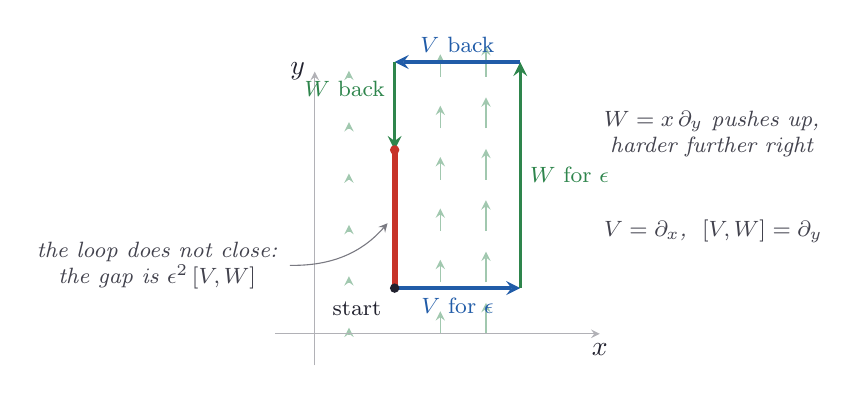
\begin{tikzpicture}[ink/.style={line width=0.9pt, ndInk}, faint/.style={line width=0.4pt, ndInk!35}, dashedink/.style={line width=0.5pt, ndInk!55, dash pattern=on 2.5pt off 2pt}, vec/.style={->, >=stealth, line width=1.2pt}, note/.style={font=\footnotesize\itshape, text=ndInk!85, align=center}, pointer/.style={->, >=stealth, line width=0.4pt, ndInk!60, shorten >=2pt, shorten <=1pt}, dot/.style={circle, fill=ndInk, inner sep=0pt, minimum size=3.4pt}, wash/.style={fill=ndSky, fill opacity=0.55}, every node/.style={text=ndInk}]
\definecolor{ndInk}{rgb}{0.13,0.13,0.18}
\definecolor{ndPaper}{rgb}{0.99,0.96,0.88}
\definecolor{ndSky}{rgb}{0.84,0.91,0.98}
\definecolor{ndRose}{rgb}{0.98,0.86,0.84}
\definecolor{ndBlue}{rgb}{0.13,0.36,0.66}
\definecolor{ndRed}{rgb}{0.78,0.20,0.16}
\definecolor{ndGold}{rgb}{0.88,0.62,0.10}
\definecolor{ndGreen}{rgb}{0.18,0.52,0.30}
\draw[->, >=stealth, line width=0.5pt, ndGreen!45] (0.435,0.000) -- (0.435,0.078);
\draw[->, >=stealth, line width=0.5pt, ndGreen!45] (0.435,0.652) -- (0.435,0.731);
\draw[->, >=stealth, line width=0.5pt, ndGreen!45] (0.435,1.305) -- (0.435,1.383);
\draw[->, >=stealth, line width=0.5pt, ndGreen!45] (0.435,1.958) -- (0.435,2.036);
\draw[->, >=stealth, line width=0.5pt, ndGreen!45] (0.435,2.610) -- (0.435,2.688);
\draw[->, >=stealth, line width=0.5pt, ndGreen!45] (0.435,3.262) -- (0.435,3.341);
\draw[->, >=stealth, line width=0.5pt, ndGreen!45] (1.595,0.000) -- (1.595,0.287);
\draw[->, >=stealth, line width=0.5pt, ndGreen!45] (1.595,0.652) -- (1.595,0.940);
\draw[->, >=stealth, line width=0.5pt, ndGreen!45] (1.595,1.305) -- (1.595,1.592);
\draw[->, >=stealth, line width=0.5pt, ndGreen!45] (1.595,1.958) -- (1.595,2.245);
\draw[->, >=stealth, line width=0.5pt, ndGreen!45] (1.595,2.610) -- (1.595,2.897);
\draw[->, >=stealth, line width=0.5pt, ndGreen!45] (1.595,3.262) -- (1.595,3.550);
\draw[->, >=stealth, line width=0.5pt, ndGreen!45] (2.175,0.000) -- (2.175,0.392);
\draw[->, >=stealth, line width=0.5pt, ndGreen!45] (2.175,0.652) -- (2.175,1.044);
\draw[->, >=stealth, line width=0.5pt, ndGreen!45] (2.175,1.305) -- (2.175,1.696);
\draw[->, >=stealth, line width=0.5pt, ndGreen!45] (2.175,1.958) -- (2.175,2.349);
\draw[->, >=stealth, line width=0.5pt, ndGreen!45] (2.175,2.610) -- (2.175,3.002);
\draw[->, >=stealth, line width=0.5pt, ndGreen!45] (2.175,3.262) -- (2.175,3.654);
\draw[faint, ->, >=stealth] (-0.50,0) -- (3.62,0) node[below] {$x$};
\draw[faint, ->, >=stealth] (0,-0.40) -- (0,3.33) node[left] {$y$};
\draw[vec, ndBlue] (1.015,0.580) -- (2.610,0.580);
\node[below, font=\footnotesize, text=ndBlue] at (1.812,0.580) {$V$ for $\epsilon$};
\draw[vec, ndGreen] (2.610,0.580) -- (2.610,3.451);
\node[right, font=\footnotesize, text=ndGreen] at (2.610,2.016) {$W$ for $\epsilon$};
\draw[vec, ndBlue] (2.610,3.451) -- (1.015,3.451);
\node[above, font=\footnotesize, text=ndBlue] at (1.812,3.451) {$V$ back};
\draw[vec, ndGreen] (1.015,3.451) -- (1.015,2.335);
\node[left, font=\footnotesize, text=ndGreen] at (1.015,3.116) {$W$ back};
\draw[line width=2.2pt, ndRed] (1.015,0.580) -- (1.015,2.335);
\node[dot, label={[font=\footnotesize]below left:start}] at (1.015,0.580) {};
\node[dot, fill=ndRed] at (1.015,2.335) {};
\node[note, anchor=east] (g) at (-0.35,0.87) {the loop does not close:\\the gap is $\epsilon^2\,[V,W]$};
\draw[pointer] (g.east) to[bend right=25] (0.971,1.457);
\node[note, anchor=west] (w) at (3.55,2.54) {$W=x\,\partial_y$ pushes up,\\harder further right};
\node[note, anchor=west] at (3.55,1.30) {$V=\partial_x$, $\;[V,W]=\partial_y$};
\end{tikzpicture}
}
\caption{The flows of $V=\partial_x$ (blue) and $W=x\,\partial_y$ (green, drawn faintly as a field) do not commute: the loop $V$, $W$, $-V$, $-W$ misses its start by $\epsilon^2\comm{V}{W}=\epsilon^2\partial_y$ (red). Generated by \texttt{code/ch02\_jacobi.py}.}\label{fig:ch02:jacobi}
\end{figure}}
\onp{\begin{center}\resizebox{!}{0.5\textheight}{% Generated by code/needham.py -- do not edit by hand.
\definecolor{qocA}{rgb}{0.00,0.45,0.70}
\definecolor{qocB}{rgb}{0.90,0.60,0.00}
\definecolor{qocC}{rgb}{0.00,0.62,0.45}
\definecolor{qocD}{rgb}{0.80,0.40,0.00}
\definecolor{qocE}{rgb}{0.80,0.60,0.70}
\definecolor{qocF}{rgb}{0.35,0.70,0.90}
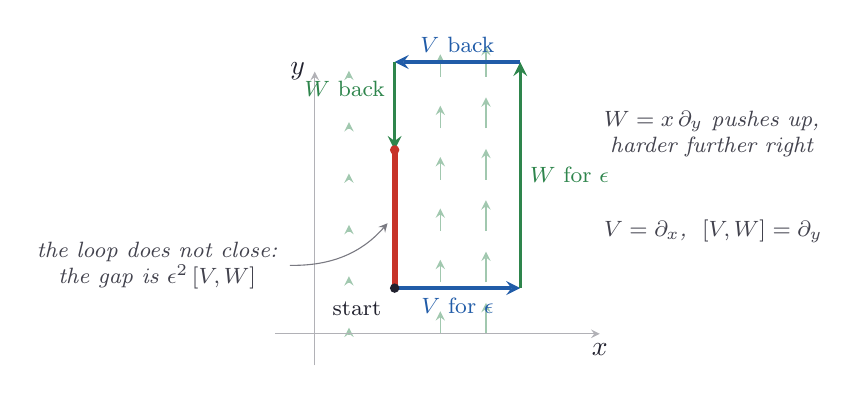
\begin{tikzpicture}[ink/.style={line width=0.9pt, ndInk}, faint/.style={line width=0.4pt, ndInk!35}, dashedink/.style={line width=0.5pt, ndInk!55, dash pattern=on 2.5pt off 2pt}, vec/.style={->, >=stealth, line width=1.2pt}, note/.style={font=\footnotesize\itshape, text=ndInk!85, align=center}, pointer/.style={->, >=stealth, line width=0.4pt, ndInk!60, shorten >=2pt, shorten <=1pt}, dot/.style={circle, fill=ndInk, inner sep=0pt, minimum size=3.4pt}, wash/.style={fill=ndSky, fill opacity=0.55}, every node/.style={text=ndInk}]
\definecolor{ndInk}{rgb}{0.13,0.13,0.18}
\definecolor{ndPaper}{rgb}{0.99,0.96,0.88}
\definecolor{ndSky}{rgb}{0.84,0.91,0.98}
\definecolor{ndRose}{rgb}{0.98,0.86,0.84}
\definecolor{ndBlue}{rgb}{0.13,0.36,0.66}
\definecolor{ndRed}{rgb}{0.78,0.20,0.16}
\definecolor{ndGold}{rgb}{0.88,0.62,0.10}
\definecolor{ndGreen}{rgb}{0.18,0.52,0.30}
\draw[->, >=stealth, line width=0.5pt, ndGreen!45] (0.435,0.000) -- (0.435,0.078);
\draw[->, >=stealth, line width=0.5pt, ndGreen!45] (0.435,0.652) -- (0.435,0.731);
\draw[->, >=stealth, line width=0.5pt, ndGreen!45] (0.435,1.305) -- (0.435,1.383);
\draw[->, >=stealth, line width=0.5pt, ndGreen!45] (0.435,1.958) -- (0.435,2.036);
\draw[->, >=stealth, line width=0.5pt, ndGreen!45] (0.435,2.610) -- (0.435,2.688);
\draw[->, >=stealth, line width=0.5pt, ndGreen!45] (0.435,3.262) -- (0.435,3.341);
\draw[->, >=stealth, line width=0.5pt, ndGreen!45] (1.595,0.000) -- (1.595,0.287);
\draw[->, >=stealth, line width=0.5pt, ndGreen!45] (1.595,0.652) -- (1.595,0.940);
\draw[->, >=stealth, line width=0.5pt, ndGreen!45] (1.595,1.305) -- (1.595,1.592);
\draw[->, >=stealth, line width=0.5pt, ndGreen!45] (1.595,1.958) -- (1.595,2.245);
\draw[->, >=stealth, line width=0.5pt, ndGreen!45] (1.595,2.610) -- (1.595,2.897);
\draw[->, >=stealth, line width=0.5pt, ndGreen!45] (1.595,3.262) -- (1.595,3.550);
\draw[->, >=stealth, line width=0.5pt, ndGreen!45] (2.175,0.000) -- (2.175,0.392);
\draw[->, >=stealth, line width=0.5pt, ndGreen!45] (2.175,0.652) -- (2.175,1.044);
\draw[->, >=stealth, line width=0.5pt, ndGreen!45] (2.175,1.305) -- (2.175,1.696);
\draw[->, >=stealth, line width=0.5pt, ndGreen!45] (2.175,1.958) -- (2.175,2.349);
\draw[->, >=stealth, line width=0.5pt, ndGreen!45] (2.175,2.610) -- (2.175,3.002);
\draw[->, >=stealth, line width=0.5pt, ndGreen!45] (2.175,3.262) -- (2.175,3.654);
\draw[faint, ->, >=stealth] (-0.50,0) -- (3.62,0) node[below] {$x$};
\draw[faint, ->, >=stealth] (0,-0.40) -- (0,3.33) node[left] {$y$};
\draw[vec, ndBlue] (1.015,0.580) -- (2.610,0.580);
\node[below, font=\footnotesize, text=ndBlue] at (1.812,0.580) {$V$ for $\epsilon$};
\draw[vec, ndGreen] (2.610,0.580) -- (2.610,3.451);
\node[right, font=\footnotesize, text=ndGreen] at (2.610,2.016) {$W$ for $\epsilon$};
\draw[vec, ndBlue] (2.610,3.451) -- (1.015,3.451);
\node[above, font=\footnotesize, text=ndBlue] at (1.812,3.451) {$V$ back};
\draw[vec, ndGreen] (1.015,3.451) -- (1.015,2.335);
\node[left, font=\footnotesize, text=ndGreen] at (1.015,3.116) {$W$ back};
\draw[line width=2.2pt, ndRed] (1.015,0.580) -- (1.015,2.335);
\node[dot, label={[font=\footnotesize]below left:start}] at (1.015,0.580) {};
\node[dot, fill=ndRed] at (1.015,2.335) {};
\node[note, anchor=east] (g) at (-0.35,0.87) {the loop does not close:\\the gap is $\epsilon^2\,[V,W]$};
\draw[pointer] (g.east) to[bend right=25] (0.971,1.457);
\node[note, anchor=west] (w) at (3.55,2.54) {$W=x\,\partial_y$ pushes up,\\harder further right};
\node[note, anchor=west] at (3.55,1.30) {$V=\partial_x$, $\;[V,W]=\partial_y$};
\end{tikzpicture}
}\end{center}}
\end{frame}

\begin{frame}\ft{$\Un[N]$, $\SU[N]$, and their Lie algebras}
\begin{defn}\label{def:ch02:lie}
$\Un[N]=\{U\in\C^{N\times N}: U^\dagger U=\Id\}$ and $\SU[N]=\{U\in\Un[N]:\det U=1\}$ are compact Lie groups of real dimension $N^2$ and $N^2-1$. Their Lie algebras are $\lieu[N]=\{X: X^\dagger=-X\}$ and $\liesu[N]=\{X\in\lieu[N]:\Tr X=0\}$, with the commutator bracket $\comm{X}{Y}=XY-YX$ and exponential map $X\mapsto\ee^{X}$.
\end{defn}
\ona{A Lie group is a group that is also a smooth manifold, with smooth multiplication and inversion. Its Lie algebra is the tangent space at $\Id$. For matrix groups there is a convenient description, provided the group is \emph{closed}. By Cartan's closed-subgroup theorem, every closed subgroup $G$ of the invertible matrices is a Lie group, and its Lie algebra is $\{X:\ee^{tX}\in G\ \text{for all}\ t\in\R\}$, with the commutator as bracket. The hypothesis is not idle. In the torus $T^2=\{\operatorname{diag}(\ee^{\imath\alpha},\ee^{\imath\beta})\}\subset\Un[2]$, the one-parameter group $t\mapsto\operatorname{diag}(\ee^{\imath t},\ee^{\imath\sqrt2t})$ never closes up, because $\sqrt2$ is irrational, and it winds densely around the torus. It is a Lie group in its own right, with Lie algebra $\R\cdot\operatorname{diag}(\imath,\imath\sqrt2)$, but it is not closed, and its topology as a group (a line) differs from the one inherited from $\Un[2]$. Subgroups of this kind, images of Lie groups under injective homomorphisms, are called \emph{immersed}, and they appear in Theorem~\ref{thm:js-preview}.}
\ona{Hamiltonians are Hermitian, so $-\imath H\in\lieu[N]$. Every Hamiltonian splits as $H=H'+\tfrac{\Tr H}{N}\Id$ with $H'$ traceless, and since $\Id$ commutes with everything, the trace part only multiplies the propagator by the global phase $\ee^{-\imath\int\Tr H(s)\,\mathrm ds/N}$. We may therefore drop it and work with traceless Hamiltonians, i.e.\ in $\liesu[N]$. On the level of Lie algebras this is clean: $\lieu[N]=\liesu[N]\oplus\imath\R\Id$ is a direct sum, and the two summands commute. On the level of groups it is not: every $U\in\Un[N]$ can be written as $\ee^{\imath\varphi}V$ with $V\in\SU[N]$, but not uniquely, because $\ee^{\imath\varphi}V=\ee^{\imath\varphi'}V'$ whenever $V'=\omega V$ for an $N$-th root of unity $\omega$ (which lies in $\SU[N]$ since $\det(\omega\Id)=\omega^N=1$). Hence $\Un[N]\cong(\Un[1]\times\SU[N])/\mathbb Z_N$, not a direct product. Gates up to a global phase form the \emph{projective unitary group} $\mathrm{PU}(N)=\Un[N]/\Un[1]=\SU[N]/\mathbb Z_N$, the natural home of the phase-invariant costs of Section~\ref{sec:ch02:problems}. A basis of $\liesu[2]$ is $\{-\imath\sigma_x/2,-\imath\sigma_y/2,-\imath\sigma_z/2\}$, and by \eqref{eq:ch02:pauli-comm} its brackets are $\comm{-\imath\sigx/2}{-\imath\sigy/2}=-\tfrac14\comm{\sigx}{\sigy}=-\tfrac{\imath}{2}\sigz$ and cyclically: the bracket of two basis elements is the third, as for the cross product of unit vectors in $\R^3$. A basis of $\liesu[2^q]$ is given by $-\imath$ times the $4^q-1$ non-identity Pauli strings.}
\begin{defn}[Dynamical Lie algebra]\label{def:dla}
Given a drift Hamiltonian $\Hdrift$ and control Hamiltonians $\Hctrl[1],\dots,\Hctrl[m]$ (Section~\ref{sec:ch02:bilinear}), the dynamical Lie algebra is
\[\Lie\{-\imath\Hdrift,-\imath\Hctrl[1],\dots,-\imath\Hctrl[m]\},\]
the smallest Lie subalgebra of $\lieu[N]$ containing the generators.
\end{defn}
\onp{The dynamical Lie algebra decides controllability (\Chap~\ref{C.StateSpace}).}
\end{frame}

\begin{frame}\ft{A Lie group and its Lie algebra, pictured}
\ona{The groups we care about cannot be drawn: $\SU[2]$ is the three-sphere, and $\Un[N]$ has dimension $N^2$. Nor can one draw a Lie group as an ordinary sphere $S^2$: a Lie group has a nowhere-vanishing vector field (translate any nonzero $X\in\mathfrak g$ around the group), whereas by the hairy ball theorem every vector field on $S^2$ vanishes somewhere. The only spheres that are Lie groups are $S^0$, $S^1$ and $S^3$. Figure~\ref{fig:ch02:group} therefore shows an honest, if commutative, example: the nonzero complex numbers $G=\C^\times$ under multiplication. Writing $z=\ee^{s+\imath\varphi}$, we draw $z$ on a cylinder at angle $\varphi=\arg z$ and height $s=\log\abs z$. The identity is the point $1$. The Lie algebra $\mathfrak g=\C$ is the tangent plane there: the set of all velocities with which a curve in $G$ can leave $1$. The exponential map turns a velocity $X=a+\imath b$ into the one-parameter subgroup $t\mapsto\ee^{tX}=\ee^{ta}\ee^{\imath tb}$, which leaves $1$ with velocity $X$. On the cylinder it is a helix, climbing by $a$ while turning by $b$ per unit of $t$; unrolling the cylinder into a plane turns every helix into a straight line, which is the precise sense in which one-parameter subgroups ``keep going straight''. Two helices are special. $X=\imath$ gives the circle $\Un[1]$, which closes up because $\ee^{2\pi\imath}=1$: the exponential map is not injective. $X=1$ gives the positive reals. Since $\ee^{sX}\ee^{tX}=\ee^{(s+t)X}$, equal steps in $t$ give equally spaced points.}
\ona{\begin{figure}[h]\centering
\resizebox{0.85\linewidth}{!}{% Generated by code/needham.py -- do not edit by hand.
\definecolor{qocA}{rgb}{0.00,0.45,0.70}
\definecolor{qocB}{rgb}{0.90,0.60,0.00}
\definecolor{qocC}{rgb}{0.00,0.62,0.45}
\definecolor{qocD}{rgb}{0.80,0.40,0.00}
\definecolor{qocE}{rgb}{0.80,0.60,0.70}
\definecolor{qocF}{rgb}{0.35,0.70,0.90}
\begin{tikzpicture}[ink/.style={line width=0.9pt, ndInk}, faint/.style={line width=0.4pt, ndInk!35}, dashedink/.style={line width=0.5pt, ndInk!55, dash pattern=on 2.5pt off 2pt}, vec/.style={->, >=stealth, line width=1.2pt}, note/.style={font=\footnotesize\itshape, text=ndInk!85, align=center}, pointer/.style={->, >=stealth, line width=0.4pt, ndInk!60, shorten >=2pt, shorten <=1pt}, dot/.style={circle, fill=ndInk, inner sep=0pt, minimum size=3.4pt}, wash/.style={fill=ndSky, fill opacity=0.55}, every node/.style={text=ndInk}]
\definecolor{ndInk}{rgb}{0.13,0.13,0.18}
\definecolor{ndPaper}{rgb}{0.99,0.96,0.88}
\definecolor{ndSky}{rgb}{0.84,0.91,0.98}
\definecolor{ndRose}{rgb}{0.98,0.86,0.84}
\definecolor{ndBlue}{rgb}{0.13,0.36,0.66}
\definecolor{ndRed}{rgb}{0.78,0.20,0.16}
\definecolor{ndGold}{rgb}{0.88,0.62,0.10}
\definecolor{ndGreen}{rgb}{0.18,0.52,0.30}
\shade[ball color=ndSky!70!white, opacity=0.45] (0.000,0.000) circle (2.400);
\draw[ink] (0.000,0.000) circle (2.400);
\draw[faint] (2.078,-0.488) -- (2.109,-0.466) -- (2.138,-0.443) -- (2.166,-0.420) -- (2.193,-0.397) -- (2.217,-0.374) -- (2.241,-0.350) -- (2.262,-0.326) -- (2.283,-0.302) -- (2.301,-0.277) -- (2.318,-0.253) -- (2.334,-0.228) -- (2.348,-0.203) -- (2.360,-0.178) -- (2.370,-0.153) -- (2.379,-0.127) -- (2.387,-0.102) -- (2.393,-0.077) -- (2.397,-0.051) -- (2.399,-0.026) -- (2.400,0.000);
\draw[faint] (-2.400,0.000) -- (-2.399,-0.026) -- (-2.397,-0.051) -- (-2.393,-0.077) -- (-2.387,-0.102) -- (-2.379,-0.127) -- (-2.370,-0.153) -- (-2.360,-0.178) -- (-2.348,-0.203) -- (-2.334,-0.228) -- (-2.318,-0.253) -- (-2.301,-0.277) -- (-2.283,-0.302) -- (-2.262,-0.326) -- (-2.241,-0.350) -- (-2.217,-0.374) -- (-2.193,-0.397) -- (-2.166,-0.420) -- (-2.138,-0.443) -- (-2.109,-0.466) -- (-2.078,-0.488) -- (-2.046,-0.510) -- (-2.013,-0.532) -- (-1.978,-0.553) -- (-1.942,-0.574) -- (-1.904,-0.594) -- (-1.865,-0.614) -- (-1.825,-0.634) -- (-1.784,-0.653) -- (-1.741,-0.672) -- (-1.697,-0.690) -- (-1.652,-0.708) -- (-1.606,-0.725) -- (-1.559,-0.742) -- (-1.510,-0.759) -- (-1.461,-0.774) -- (-1.411,-0.790) -- (-1.359,-0.804) -- (-1.307,-0.819) -- (-1.254,-0.832) -- (-1.200,-0.845) -- (-1.145,-0.858) -- (-1.090,-0.870) -- (-1.033,-0.881) -- (-0.976,-0.892) -- (-0.918,-0.902) -- (-0.860,-0.911) -- (-0.801,-0.920) -- (-0.742,-0.928) -- (-0.682,-0.936) -- (-0.621,-0.943) -- (-0.560,-0.949) -- (-0.499,-0.955) -- (-0.437,-0.960) -- (-0.375,-0.964) -- (-0.313,-0.968) -- (-0.251,-0.971) -- (-0.188,-0.973) -- (-0.126,-0.975) -- (-0.063,-0.976) -- (-0.000,-0.976) -- (0.063,-0.976) -- (0.126,-0.975) -- (0.188,-0.973) -- (0.251,-0.971) -- (0.313,-0.968) -- (0.375,-0.964) -- (0.437,-0.960) -- (0.499,-0.955) -- (0.560,-0.949) -- (0.621,-0.943) -- (0.682,-0.936) -- (0.742,-0.928) -- (0.801,-0.920) -- (0.860,-0.911) -- (0.918,-0.902) -- (0.976,-0.892) -- (1.033,-0.881) -- (1.090,-0.870) -- (1.145,-0.858) -- (1.200,-0.845) -- (1.254,-0.832) -- (1.307,-0.819) -- (1.359,-0.804) -- (1.411,-0.790) -- (1.461,-0.774) -- (1.510,-0.759) -- (1.559,-0.742) -- (1.606,-0.725) -- (1.652,-0.708) -- (1.697,-0.690) -- (1.741,-0.672) -- (1.784,-0.653) -- (1.825,-0.634) -- (1.865,-0.614) -- (1.904,-0.594) -- (1.942,-0.574) -- (1.978,-0.553) -- (2.013,-0.532) -- (2.046,-0.510) -- (2.078,-0.488);
\draw[faint, densely dotted] (2.399,0.026) -- (2.397,0.051) -- (2.393,0.077) -- (2.387,0.102) -- (2.379,0.127) -- (2.370,0.153) -- (2.360,0.178) -- (2.348,0.203) -- (2.334,0.228) -- (2.318,0.253) -- (2.301,0.277) -- (2.283,0.302) -- (2.262,0.326) -- (2.241,0.350) -- (2.217,0.374) -- (2.193,0.397) -- (2.166,0.420) -- (2.138,0.443) -- (2.109,0.466) -- (2.078,0.488) -- (2.046,0.510) -- (2.013,0.532) -- (1.978,0.553) -- (1.942,0.574) -- (1.904,0.594) -- (1.865,0.614) -- (1.825,0.634) -- (1.784,0.653) -- (1.741,0.672) -- (1.697,0.690) -- (1.652,0.708) -- (1.606,0.725) -- (1.559,0.742) -- (1.510,0.759) -- (1.461,0.774) -- (1.411,0.790) -- (1.359,0.804) -- (1.307,0.819) -- (1.254,0.832) -- (1.200,0.845) -- (1.145,0.858) -- (1.090,0.870) -- (1.033,0.881) -- (0.976,0.892) -- (0.918,0.902) -- (0.860,0.911) -- (0.801,0.920) -- (0.742,0.928) -- (0.682,0.936) -- (0.621,0.943) -- (0.560,0.949) -- (0.499,0.955) -- (0.437,0.960) -- (0.375,0.964) -- (0.313,0.968) -- (0.251,0.971) -- (0.188,0.973) -- (0.126,0.975) -- (0.063,0.976) -- (0.000,0.976) -- (-0.063,0.976) -- (-0.126,0.975) -- (-0.188,0.973) -- (-0.251,0.971) -- (-0.313,0.968) -- (-0.375,0.964) -- (-0.437,0.960) -- (-0.499,0.955) -- (-0.560,0.949) -- (-0.621,0.943) -- (-0.682,0.936) -- (-0.742,0.928) -- (-0.801,0.920) -- (-0.860,0.911) -- (-0.918,0.902) -- (-0.976,0.892) -- (-1.033,0.881) -- (-1.090,0.870) -- (-1.145,0.858) -- (-1.200,0.845) -- (-1.254,0.832) -- (-1.307,0.819) -- (-1.359,0.804) -- (-1.411,0.790) -- (-1.461,0.774) -- (-1.510,0.759) -- (-1.559,0.742) -- (-1.606,0.725) -- (-1.652,0.708) -- (-1.697,0.690) -- (-1.741,0.672) -- (-1.784,0.653) -- (-1.825,0.634) -- (-1.865,0.614) -- (-1.904,0.594) -- (-1.942,0.574) -- (-1.978,0.553) -- (-2.013,0.532) -- (-2.046,0.510) -- (-2.078,0.488) -- (-2.109,0.466) -- (-2.138,0.443) -- (-2.166,0.420) -- (-2.193,0.397) -- (-2.217,0.374) -- (-2.241,0.350) -- (-2.262,0.326) -- (-2.283,0.302) -- (-2.301,0.277) -- (-2.318,0.253) -- (-2.334,0.228) -- (-2.348,0.203) -- (-2.360,0.178) -- (-2.370,0.153) -- (-2.379,0.127) -- (-2.387,0.102) -- (-2.393,0.077) -- (-2.397,0.051) -- (-2.399,0.026);
\filldraw[fill=ndPaper, fill opacity=0.85, draw=ndInk!70, line width=0.6pt] (-0.703,3.259) -- (-2.623,1.907) -- (0.703,1.126) -- (2.623,2.478) -- cycle;
\node[anchor=north east] at (-0.703,3.259) {$\mathfrak g=T_{\Id}G$};
\draw[line width=1.1pt, ndBlue!75] (0.000,2.193) -- (-0.029,2.182) -- (-0.058,2.171) -- (-0.086,2.160) -- (-0.115,2.148) -- (-0.144,2.135) -- (-0.172,2.122) -- (-0.201,2.109) -- (-0.230,2.095) -- (-0.258,2.080) -- (-0.287,2.065) -- (-0.315,2.049) -- (-0.343,2.033) -- (-0.372,2.016) -- (-0.400,1.999) -- (-0.428,1.981) -- (-0.456,1.963) -- (-0.483,1.944) -- (-0.511,1.925) -- (-0.539,1.906) -- (-0.566,1.886) -- (-0.593,1.865) -- (-0.621,1.844) -- (-0.648,1.822) -- (-0.674,1.800) -- (-0.701,1.778) -- (-0.727,1.755) -- (-0.754,1.732) -- (-0.780,1.708) -- (-0.806,1.684) -- (-0.832,1.659) -- (-0.857,1.634) -- (-0.882,1.609) -- (-0.907,1.583) -- (-0.932,1.557) -- (-0.957,1.530) -- (-0.981,1.503) -- (-1.005,1.476) -- (-1.029,1.448) -- (-1.053,1.420) -- (-1.076,1.391) -- (-1.099,1.362) -- (-1.122,1.333) -- (-1.144,1.304) -- (-1.167,1.274) -- (-1.189,1.244) -- (-1.210,1.213) -- (-1.232,1.183) -- (-1.253,1.152) -- (-1.273,1.120) -- (-1.294,1.089) -- (-1.314,1.057) -- (-1.334,1.025) -- (-1.353,0.992) -- (-1.372,0.960) -- (-1.391,0.927) -- (-1.409,0.893) -- (-1.427,0.860) -- (-1.445,0.827) -- (-1.462,0.793) -- (-1.479,0.759) -- (-1.496,0.725) -- (-1.512,0.690) -- (-1.528,0.656) -- (-1.543,0.621) -- (-1.558,0.586) -- (-1.573,0.551) -- (-1.587,0.516) -- (-1.601,0.481) -- (-1.614,0.446) -- (-1.628,0.410) -- (-1.640,0.374) -- (-1.652,0.339) -- (-1.664,0.303) -- (-1.676,0.267) -- (-1.687,0.231) -- (-1.697,0.195) -- (-1.707,0.159) -- (-1.717,0.123) -- (-1.726,0.087);
\draw[vec, ndBlue] (0.000,2.193) -- (-0.764,1.925) node[below left] {$X$};
\fill[ndBlue] (-0.742,1.742) circle (1.5pt);
\fill[ndBlue] (-1.355,0.989) circle (1.5pt);
\fill[ndBlue] (-1.732,0.064) circle (1.5pt);
\node[ndBlue, below right] at (-1.732,0.064) {$\ee^{3X}$};
\draw[line width=1.1pt, ndRed!75] (0.000,2.193) -- (0.037,2.188) -- (0.073,2.183) -- (0.109,2.177) -- (0.146,2.171) -- (0.182,2.164) -- (0.219,2.157) -- (0.255,2.149) -- (0.291,2.141) -- (0.327,2.132) -- (0.364,2.123) -- (0.400,2.113) -- (0.435,2.102) -- (0.471,2.091) -- (0.507,2.080) -- (0.543,2.068) -- (0.578,2.055) -- (0.613,2.042) -- (0.648,2.029) -- (0.683,2.015) -- (0.718,2.000) -- (0.753,1.985) -- (0.787,1.969) -- (0.821,1.953) -- (0.855,1.937) -- (0.889,1.920) -- (0.923,1.902) -- (0.956,1.884) -- (0.989,1.866) -- (1.022,1.847) -- (1.055,1.827) -- (1.087,1.808) -- (1.119,1.787) -- (1.151,1.766) -- (1.182,1.745) -- (1.214,1.724) -- (1.244,1.702) -- (1.275,1.679) -- (1.305,1.656) -- (1.335,1.633) -- (1.365,1.609) -- (1.394,1.585) -- (1.423,1.560) -- (1.452,1.535) -- (1.480,1.510) -- (1.508,1.484) -- (1.535,1.458) -- (1.562,1.432) -- (1.589,1.405) -- (1.615,1.378) -- (1.641,1.350) -- (1.666,1.323) -- (1.691,1.295) -- (1.716,1.266) -- (1.740,1.237) -- (1.764,1.208) -- (1.787,1.179) -- (1.810,1.149) -- (1.833,1.119) -- (1.855,1.089) -- (1.876,1.058) -- (1.897,1.027) -- (1.918,0.996) -- (1.938,0.965) -- (1.957,0.933) -- (1.976,0.902) -- (1.995,0.870) -- (2.013,0.837) -- (2.031,0.805) -- (2.048,0.772) -- (2.064,0.739) -- (2.080,0.706) -- (2.096,0.673) -- (2.111,0.640) -- (2.125,0.606) -- (2.139,0.573) -- (2.153,0.539) -- (2.166,0.505) -- (2.178,0.471) -- (2.190,0.437);
\draw[vec, ndRed] (0.000,2.193) -- (0.969,2.080) node[above] {$Y$};
\fill[ndRed] (0.941,1.892) circle (1.5pt);
\fill[ndRed] (1.718,1.264) circle (1.5pt);
\fill[ndRed] (2.197,0.415) circle (1.5pt);
\node[ndRed, above right] at (2.197,0.415) {$\ee^{3Y}$};
\node[dot, label={[label distance=1pt]above:$\Id$}] at (0.000,2.193) {};
\node at (-1.803,-1.622) {$G$};
\node[note, anchor=west] (n1) at (3.7,2.5) {the Lie algebra: all\\ velocities at $\Id$};
\draw[pointer] (n1.west) to[bend right=15] (0.287,1.223);
\node[note, anchor=west] (n2) at (3.7,0.5) {$t\mapsto\ee^{tX}$: set off from $\Id$\\with velocity $X$ and keep\\ going ``straight''};
\draw[pointer] (n2.west) to[bend left=15] (-1.240,1.170);
\node[note, anchor=west] (n3) at (3.7,-1.5) {dots: equal steps of $t$;\\$\ee^{sX}\ee^{tX}=\ee^{(s+t)X}$};
\end{tikzpicture}
}
\caption{The Lie group $\C^\times$, drawn as a cylinder (angle $\arg z$, height $\log\abs z$), its Lie algebra $\mathfrak g=\C$ as the tangent plane at $1$, and three one-parameter subgroups: the circle $\Un[1]=\{\ee^{\imath t}\}$ (blue), the positive reals $\{\ee^{t}\}$ (green), and the helix $\ee^{t(0.25+\imath)}$ (red, dots at $t=1,2,\dots$). Generated by \texttt{code/ch02\_group.py}.}\label{fig:ch02:group}
\end{figure}}
\onp{\begin{center}\resizebox{!}{0.68\textheight}{% Generated by code/needham.py -- do not edit by hand.
\definecolor{qocA}{rgb}{0.00,0.45,0.70}
\definecolor{qocB}{rgb}{0.90,0.60,0.00}
\definecolor{qocC}{rgb}{0.00,0.62,0.45}
\definecolor{qocD}{rgb}{0.80,0.40,0.00}
\definecolor{qocE}{rgb}{0.80,0.60,0.70}
\definecolor{qocF}{rgb}{0.35,0.70,0.90}
\begin{tikzpicture}[ink/.style={line width=0.9pt, ndInk}, faint/.style={line width=0.4pt, ndInk!35}, dashedink/.style={line width=0.5pt, ndInk!55, dash pattern=on 2.5pt off 2pt}, vec/.style={->, >=stealth, line width=1.2pt}, note/.style={font=\footnotesize\itshape, text=ndInk!85, align=center}, pointer/.style={->, >=stealth, line width=0.4pt, ndInk!60, shorten >=2pt, shorten <=1pt}, dot/.style={circle, fill=ndInk, inner sep=0pt, minimum size=3.4pt}, wash/.style={fill=ndSky, fill opacity=0.55}, every node/.style={text=ndInk}]
\definecolor{ndInk}{rgb}{0.13,0.13,0.18}
\definecolor{ndPaper}{rgb}{0.99,0.96,0.88}
\definecolor{ndSky}{rgb}{0.84,0.91,0.98}
\definecolor{ndRose}{rgb}{0.98,0.86,0.84}
\definecolor{ndBlue}{rgb}{0.13,0.36,0.66}
\definecolor{ndRed}{rgb}{0.78,0.20,0.16}
\definecolor{ndGold}{rgb}{0.88,0.62,0.10}
\definecolor{ndGreen}{rgb}{0.18,0.52,0.30}
\shade[ball color=ndSky!70!white, opacity=0.45] (0.000,0.000) circle (2.400);
\draw[ink] (0.000,0.000) circle (2.400);
\draw[faint] (2.078,-0.488) -- (2.109,-0.466) -- (2.138,-0.443) -- (2.166,-0.420) -- (2.193,-0.397) -- (2.217,-0.374) -- (2.241,-0.350) -- (2.262,-0.326) -- (2.283,-0.302) -- (2.301,-0.277) -- (2.318,-0.253) -- (2.334,-0.228) -- (2.348,-0.203) -- (2.360,-0.178) -- (2.370,-0.153) -- (2.379,-0.127) -- (2.387,-0.102) -- (2.393,-0.077) -- (2.397,-0.051) -- (2.399,-0.026) -- (2.400,0.000);
\draw[faint] (-2.400,0.000) -- (-2.399,-0.026) -- (-2.397,-0.051) -- (-2.393,-0.077) -- (-2.387,-0.102) -- (-2.379,-0.127) -- (-2.370,-0.153) -- (-2.360,-0.178) -- (-2.348,-0.203) -- (-2.334,-0.228) -- (-2.318,-0.253) -- (-2.301,-0.277) -- (-2.283,-0.302) -- (-2.262,-0.326) -- (-2.241,-0.350) -- (-2.217,-0.374) -- (-2.193,-0.397) -- (-2.166,-0.420) -- (-2.138,-0.443) -- (-2.109,-0.466) -- (-2.078,-0.488) -- (-2.046,-0.510) -- (-2.013,-0.532) -- (-1.978,-0.553) -- (-1.942,-0.574) -- (-1.904,-0.594) -- (-1.865,-0.614) -- (-1.825,-0.634) -- (-1.784,-0.653) -- (-1.741,-0.672) -- (-1.697,-0.690) -- (-1.652,-0.708) -- (-1.606,-0.725) -- (-1.559,-0.742) -- (-1.510,-0.759) -- (-1.461,-0.774) -- (-1.411,-0.790) -- (-1.359,-0.804) -- (-1.307,-0.819) -- (-1.254,-0.832) -- (-1.200,-0.845) -- (-1.145,-0.858) -- (-1.090,-0.870) -- (-1.033,-0.881) -- (-0.976,-0.892) -- (-0.918,-0.902) -- (-0.860,-0.911) -- (-0.801,-0.920) -- (-0.742,-0.928) -- (-0.682,-0.936) -- (-0.621,-0.943) -- (-0.560,-0.949) -- (-0.499,-0.955) -- (-0.437,-0.960) -- (-0.375,-0.964) -- (-0.313,-0.968) -- (-0.251,-0.971) -- (-0.188,-0.973) -- (-0.126,-0.975) -- (-0.063,-0.976) -- (-0.000,-0.976) -- (0.063,-0.976) -- (0.126,-0.975) -- (0.188,-0.973) -- (0.251,-0.971) -- (0.313,-0.968) -- (0.375,-0.964) -- (0.437,-0.960) -- (0.499,-0.955) -- (0.560,-0.949) -- (0.621,-0.943) -- (0.682,-0.936) -- (0.742,-0.928) -- (0.801,-0.920) -- (0.860,-0.911) -- (0.918,-0.902) -- (0.976,-0.892) -- (1.033,-0.881) -- (1.090,-0.870) -- (1.145,-0.858) -- (1.200,-0.845) -- (1.254,-0.832) -- (1.307,-0.819) -- (1.359,-0.804) -- (1.411,-0.790) -- (1.461,-0.774) -- (1.510,-0.759) -- (1.559,-0.742) -- (1.606,-0.725) -- (1.652,-0.708) -- (1.697,-0.690) -- (1.741,-0.672) -- (1.784,-0.653) -- (1.825,-0.634) -- (1.865,-0.614) -- (1.904,-0.594) -- (1.942,-0.574) -- (1.978,-0.553) -- (2.013,-0.532) -- (2.046,-0.510) -- (2.078,-0.488);
\draw[faint, densely dotted] (2.399,0.026) -- (2.397,0.051) -- (2.393,0.077) -- (2.387,0.102) -- (2.379,0.127) -- (2.370,0.153) -- (2.360,0.178) -- (2.348,0.203) -- (2.334,0.228) -- (2.318,0.253) -- (2.301,0.277) -- (2.283,0.302) -- (2.262,0.326) -- (2.241,0.350) -- (2.217,0.374) -- (2.193,0.397) -- (2.166,0.420) -- (2.138,0.443) -- (2.109,0.466) -- (2.078,0.488) -- (2.046,0.510) -- (2.013,0.532) -- (1.978,0.553) -- (1.942,0.574) -- (1.904,0.594) -- (1.865,0.614) -- (1.825,0.634) -- (1.784,0.653) -- (1.741,0.672) -- (1.697,0.690) -- (1.652,0.708) -- (1.606,0.725) -- (1.559,0.742) -- (1.510,0.759) -- (1.461,0.774) -- (1.411,0.790) -- (1.359,0.804) -- (1.307,0.819) -- (1.254,0.832) -- (1.200,0.845) -- (1.145,0.858) -- (1.090,0.870) -- (1.033,0.881) -- (0.976,0.892) -- (0.918,0.902) -- (0.860,0.911) -- (0.801,0.920) -- (0.742,0.928) -- (0.682,0.936) -- (0.621,0.943) -- (0.560,0.949) -- (0.499,0.955) -- (0.437,0.960) -- (0.375,0.964) -- (0.313,0.968) -- (0.251,0.971) -- (0.188,0.973) -- (0.126,0.975) -- (0.063,0.976) -- (0.000,0.976) -- (-0.063,0.976) -- (-0.126,0.975) -- (-0.188,0.973) -- (-0.251,0.971) -- (-0.313,0.968) -- (-0.375,0.964) -- (-0.437,0.960) -- (-0.499,0.955) -- (-0.560,0.949) -- (-0.621,0.943) -- (-0.682,0.936) -- (-0.742,0.928) -- (-0.801,0.920) -- (-0.860,0.911) -- (-0.918,0.902) -- (-0.976,0.892) -- (-1.033,0.881) -- (-1.090,0.870) -- (-1.145,0.858) -- (-1.200,0.845) -- (-1.254,0.832) -- (-1.307,0.819) -- (-1.359,0.804) -- (-1.411,0.790) -- (-1.461,0.774) -- (-1.510,0.759) -- (-1.559,0.742) -- (-1.606,0.725) -- (-1.652,0.708) -- (-1.697,0.690) -- (-1.741,0.672) -- (-1.784,0.653) -- (-1.825,0.634) -- (-1.865,0.614) -- (-1.904,0.594) -- (-1.942,0.574) -- (-1.978,0.553) -- (-2.013,0.532) -- (-2.046,0.510) -- (-2.078,0.488) -- (-2.109,0.466) -- (-2.138,0.443) -- (-2.166,0.420) -- (-2.193,0.397) -- (-2.217,0.374) -- (-2.241,0.350) -- (-2.262,0.326) -- (-2.283,0.302) -- (-2.301,0.277) -- (-2.318,0.253) -- (-2.334,0.228) -- (-2.348,0.203) -- (-2.360,0.178) -- (-2.370,0.153) -- (-2.379,0.127) -- (-2.387,0.102) -- (-2.393,0.077) -- (-2.397,0.051) -- (-2.399,0.026);
\filldraw[fill=ndPaper, fill opacity=0.85, draw=ndInk!70, line width=0.6pt] (-0.703,3.259) -- (-2.623,1.907) -- (0.703,1.126) -- (2.623,2.478) -- cycle;
\node[anchor=north east] at (-0.703,3.259) {$\mathfrak g=T_{\Id}G$};
\draw[line width=1.1pt, ndBlue!75] (0.000,2.193) -- (-0.029,2.182) -- (-0.058,2.171) -- (-0.086,2.160) -- (-0.115,2.148) -- (-0.144,2.135) -- (-0.172,2.122) -- (-0.201,2.109) -- (-0.230,2.095) -- (-0.258,2.080) -- (-0.287,2.065) -- (-0.315,2.049) -- (-0.343,2.033) -- (-0.372,2.016) -- (-0.400,1.999) -- (-0.428,1.981) -- (-0.456,1.963) -- (-0.483,1.944) -- (-0.511,1.925) -- (-0.539,1.906) -- (-0.566,1.886) -- (-0.593,1.865) -- (-0.621,1.844) -- (-0.648,1.822) -- (-0.674,1.800) -- (-0.701,1.778) -- (-0.727,1.755) -- (-0.754,1.732) -- (-0.780,1.708) -- (-0.806,1.684) -- (-0.832,1.659) -- (-0.857,1.634) -- (-0.882,1.609) -- (-0.907,1.583) -- (-0.932,1.557) -- (-0.957,1.530) -- (-0.981,1.503) -- (-1.005,1.476) -- (-1.029,1.448) -- (-1.053,1.420) -- (-1.076,1.391) -- (-1.099,1.362) -- (-1.122,1.333) -- (-1.144,1.304) -- (-1.167,1.274) -- (-1.189,1.244) -- (-1.210,1.213) -- (-1.232,1.183) -- (-1.253,1.152) -- (-1.273,1.120) -- (-1.294,1.089) -- (-1.314,1.057) -- (-1.334,1.025) -- (-1.353,0.992) -- (-1.372,0.960) -- (-1.391,0.927) -- (-1.409,0.893) -- (-1.427,0.860) -- (-1.445,0.827) -- (-1.462,0.793) -- (-1.479,0.759) -- (-1.496,0.725) -- (-1.512,0.690) -- (-1.528,0.656) -- (-1.543,0.621) -- (-1.558,0.586) -- (-1.573,0.551) -- (-1.587,0.516) -- (-1.601,0.481) -- (-1.614,0.446) -- (-1.628,0.410) -- (-1.640,0.374) -- (-1.652,0.339) -- (-1.664,0.303) -- (-1.676,0.267) -- (-1.687,0.231) -- (-1.697,0.195) -- (-1.707,0.159) -- (-1.717,0.123) -- (-1.726,0.087);
\draw[vec, ndBlue] (0.000,2.193) -- (-0.764,1.925) node[below left] {$X$};
\fill[ndBlue] (-0.742,1.742) circle (1.5pt);
\fill[ndBlue] (-1.355,0.989) circle (1.5pt);
\fill[ndBlue] (-1.732,0.064) circle (1.5pt);
\node[ndBlue, below right] at (-1.732,0.064) {$\ee^{3X}$};
\draw[line width=1.1pt, ndRed!75] (0.000,2.193) -- (0.037,2.188) -- (0.073,2.183) -- (0.109,2.177) -- (0.146,2.171) -- (0.182,2.164) -- (0.219,2.157) -- (0.255,2.149) -- (0.291,2.141) -- (0.327,2.132) -- (0.364,2.123) -- (0.400,2.113) -- (0.435,2.102) -- (0.471,2.091) -- (0.507,2.080) -- (0.543,2.068) -- (0.578,2.055) -- (0.613,2.042) -- (0.648,2.029) -- (0.683,2.015) -- (0.718,2.000) -- (0.753,1.985) -- (0.787,1.969) -- (0.821,1.953) -- (0.855,1.937) -- (0.889,1.920) -- (0.923,1.902) -- (0.956,1.884) -- (0.989,1.866) -- (1.022,1.847) -- (1.055,1.827) -- (1.087,1.808) -- (1.119,1.787) -- (1.151,1.766) -- (1.182,1.745) -- (1.214,1.724) -- (1.244,1.702) -- (1.275,1.679) -- (1.305,1.656) -- (1.335,1.633) -- (1.365,1.609) -- (1.394,1.585) -- (1.423,1.560) -- (1.452,1.535) -- (1.480,1.510) -- (1.508,1.484) -- (1.535,1.458) -- (1.562,1.432) -- (1.589,1.405) -- (1.615,1.378) -- (1.641,1.350) -- (1.666,1.323) -- (1.691,1.295) -- (1.716,1.266) -- (1.740,1.237) -- (1.764,1.208) -- (1.787,1.179) -- (1.810,1.149) -- (1.833,1.119) -- (1.855,1.089) -- (1.876,1.058) -- (1.897,1.027) -- (1.918,0.996) -- (1.938,0.965) -- (1.957,0.933) -- (1.976,0.902) -- (1.995,0.870) -- (2.013,0.837) -- (2.031,0.805) -- (2.048,0.772) -- (2.064,0.739) -- (2.080,0.706) -- (2.096,0.673) -- (2.111,0.640) -- (2.125,0.606) -- (2.139,0.573) -- (2.153,0.539) -- (2.166,0.505) -- (2.178,0.471) -- (2.190,0.437);
\draw[vec, ndRed] (0.000,2.193) -- (0.969,2.080) node[above] {$Y$};
\fill[ndRed] (0.941,1.892) circle (1.5pt);
\fill[ndRed] (1.718,1.264) circle (1.5pt);
\fill[ndRed] (2.197,0.415) circle (1.5pt);
\node[ndRed, above right] at (2.197,0.415) {$\ee^{3Y}$};
\node[dot, label={[label distance=1pt]above:$\Id$}] at (0.000,2.193) {};
\node at (-1.803,-1.622) {$G$};
\node[note, anchor=west] (n1) at (3.7,2.5) {the Lie algebra: all\\ velocities at $\Id$};
\draw[pointer] (n1.west) to[bend right=15] (0.287,1.223);
\node[note, anchor=west] (n2) at (3.7,0.5) {$t\mapsto\ee^{tX}$: set off from $\Id$\\with velocity $X$ and keep\\ going ``straight''};
\draw[pointer] (n2.west) to[bend left=15] (-1.240,1.170);
\node[note, anchor=west] (n3) at (3.7,-1.5) {dots: equal steps of $t$;\\$\ee^{sX}\ee^{tX}=\ee^{(s+t)X}$};
\end{tikzpicture}
}\end{center}}
\end{frame}

\begin{frame}\ft{Brackets are new directions}
\ona{Why should commutators, rather than just linear combinations of the generators, describe what can be reached? Suppose we can switch on $-\imath H_a=X$ and $-\imath H_b=Z$ one at a time, but never a Hamiltonian proportional to $\sigy$. By the Baker--Campbell--Hausdorff formula,}
\begin{equation}\label{eq:ch02:group-commutator}
    \ee^{-\epsilon Z}\,\ee^{-\epsilon X}\,\ee^{\epsilon Z}\,\ee^{\epsilon X} \approx \ee^{\epsilon^2\comm{Z}{X}} ,
\end{equation}
\ona{so switching the two fields on and off in a loop moves the system, to leading order, along the bracket $\comm{Z}{X}$, a direction that neither field generates on its own. Iterating the construction with nested loops produces nested brackets, and in the limit every direction of the dynamical Lie algebra. Figure~\ref{fig:ch02:lie} shows this for the qubit with $X=-\imath\sigx/2$, $Z=-\imath\sigz/2$: the generators span only a plane in $\liesu[2]\cong\R^3$, but $\comm{Z}{X}=Y=-\imath\sigy/2$ completes it, so the dynamical Lie algebra is all of $\liesu[2]$. On the Bloch sphere the four legs of the loop \eqref{eq:ch02:group-commutator} fail to close, and the gap is, to leading order, the rotation $\ee^{\epsilon^2 Y}$ about the $y$-axis.}
\ona{\begin{figure}[h]\centering
\resizebox{0.9\linewidth}{!}{% Generated by code/needham.py -- do not edit by hand.
\definecolor{qocA}{rgb}{0.00,0.45,0.70}
\definecolor{qocB}{rgb}{0.90,0.60,0.00}
\definecolor{qocC}{rgb}{0.00,0.62,0.45}
\definecolor{qocD}{rgb}{0.80,0.40,0.00}
\definecolor{qocE}{rgb}{0.80,0.60,0.70}
\definecolor{qocF}{rgb}{0.35,0.70,0.90}
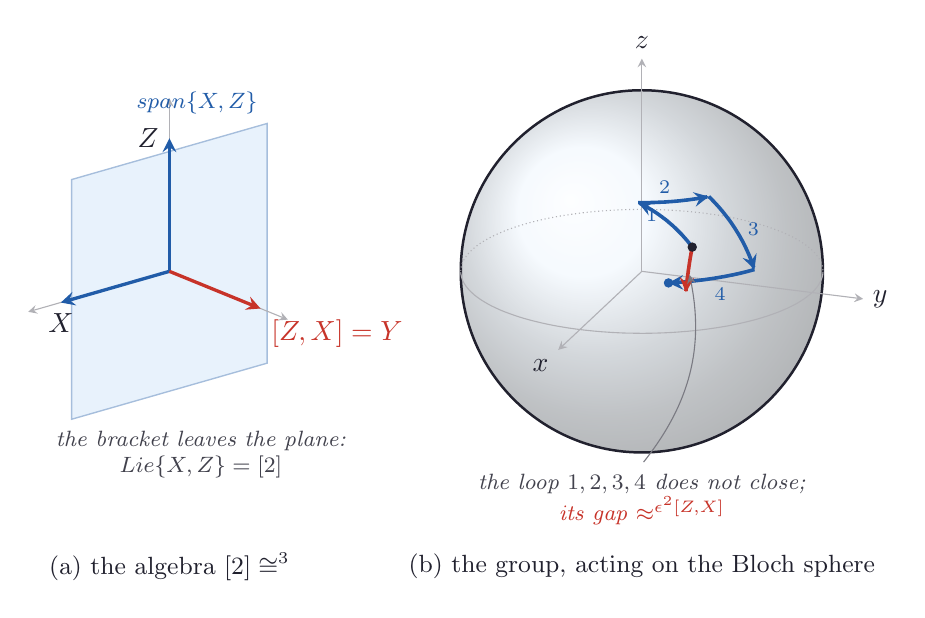
\begin{tikzpicture}[ink/.style={line width=0.9pt, ndInk}, faint/.style={line width=0.4pt, ndInk!35}, dashedink/.style={line width=0.5pt, ndInk!55, dash pattern=on 2.5pt off 2pt}, vec/.style={->, >=stealth, line width=1.2pt}, note/.style={font=\footnotesize\itshape, text=ndInk!85, align=center}, pointer/.style={->, >=stealth, line width=0.4pt, ndInk!60, shorten >=2pt, shorten <=1pt}, dot/.style={circle, fill=ndInk, inner sep=0pt, minimum size=3.4pt}, wash/.style={fill=ndSky, fill opacity=0.55}, every node/.style={text=ndInk}]
\definecolor{ndInk}{rgb}{0.13,0.13,0.18}
\definecolor{ndPaper}{rgb}{0.99,0.96,0.88}
\definecolor{ndSky}{rgb}{0.84,0.91,0.98}
\definecolor{ndRose}{rgb}{0.98,0.86,0.84}
\definecolor{ndBlue}{rgb}{0.13,0.36,0.66}
\definecolor{ndRed}{rgb}{0.78,0.20,0.16}
\definecolor{ndGold}{rgb}{0.88,0.62,0.10}
\definecolor{ndGreen}{rgb}{0.18,0.52,0.30}
\filldraw[wash, draw=ndBlue!40, line width=0.5pt] (1.241,-1.166) -- (-1.241,-1.878) -- (-1.241,1.166) -- (1.241,1.878) -- cycle;
\draw[faint, ->, >=stealth] (0.000,0.000) -- (-1.793,-0.514);
\draw[faint, ->, >=stealth] (0.000,0.000) -- (1.504,-0.613);
\draw[faint, ->, >=stealth] (0.000,0.000) -- (0.000,2.199);
\draw[vec, ndBlue] (0.000,0.000) -- (-1.379,-0.396) node[below] {$X$};
\draw[vec, ndBlue] (0.000,0.000) -- (0.000,1.691) node[left] {$Z$};
\draw[vec, ndRed] (0.000,0.000) -- (1.157,-0.472) node[below right, text=ndRed] {$[Z,X]=Y$};
\node[note, anchor=south east, text=ndBlue] at (1.241,1.878) {$\operatorname{span}\{X,Z\}$};
\node[note, anchor=north] (n) at (0.40,-1.90) {the bracket leaves the plane:\\$\operatorname{Lie}\{X,Z\}=\liesu[2]$};
\node[font=\small] at (0.00,-3.75) {(a) the algebra $\liesu[2]\cong\R^3$};
\shade[ball color=ndSky!70!white, opacity=0.45] (6.000,0.000) circle (2.300);
\draw[ink] (6.000,0.000) circle (2.300);
\draw[faint] (8.161,-0.269) -- (8.181,-0.250) -- (8.200,-0.230) -- (8.216,-0.210) -- (8.232,-0.190) -- (8.245,-0.170) -- (8.258,-0.150) -- (8.268,-0.130) -- (8.278,-0.109) -- (8.285,-0.089) -- (8.291,-0.069) -- (8.296,-0.048) -- (8.299,-0.027) -- (8.300,-0.007);
\draw[faint] (3.700,-0.014) -- (3.702,-0.034) -- (3.706,-0.055) -- (3.711,-0.075) -- (3.717,-0.096) -- (3.725,-0.116) -- (3.735,-0.137) -- (3.746,-0.157) -- (3.759,-0.177) -- (3.773,-0.197) -- (3.789,-0.217) -- (3.806,-0.237) -- (3.825,-0.256) -- (3.846,-0.275) -- (3.867,-0.295) -- (3.891,-0.314) -- (3.915,-0.332) -- (3.942,-0.351) -- (3.969,-0.369) -- (3.998,-0.387) -- (4.029,-0.405) -- (4.060,-0.423) -- (4.093,-0.440) -- (4.128,-0.457) -- (4.163,-0.473) -- (4.200,-0.490) -- (4.238,-0.506) -- (4.277,-0.521) -- (4.318,-0.536) -- (4.360,-0.551) -- (4.402,-0.566) -- (4.446,-0.580) -- (4.491,-0.594) -- (4.537,-0.607) -- (4.584,-0.620) -- (4.632,-0.632) -- (4.681,-0.644) -- (4.731,-0.656) -- (4.781,-0.667) -- (4.833,-0.678) -- (4.885,-0.688) -- (4.938,-0.698) -- (4.992,-0.707) -- (5.046,-0.716) -- (5.101,-0.724) -- (5.157,-0.732) -- (5.213,-0.739) -- (5.270,-0.746) -- (5.328,-0.752) -- (5.385,-0.758) -- (5.444,-0.763) -- (5.502,-0.768) -- (5.561,-0.772) -- (5.620,-0.776) -- (5.680,-0.779) -- (5.740,-0.782) -- (5.800,-0.784) -- (5.860,-0.785) -- (5.920,-0.786) -- (5.980,-0.787) -- (6.040,-0.787) -- (6.100,-0.786) -- (6.160,-0.785) -- (6.220,-0.783) -- (6.280,-0.781) -- (6.340,-0.778) -- (6.399,-0.775) -- (6.459,-0.771) -- (6.517,-0.766) -- (6.576,-0.762) -- (6.634,-0.756) -- (6.692,-0.750) -- (6.749,-0.744) -- (6.805,-0.737) -- (6.862,-0.729) -- (6.917,-0.721) -- (6.972,-0.713) -- (7.026,-0.704) -- (7.080,-0.695) -- (7.133,-0.685) -- (7.185,-0.674) -- (7.236,-0.663) -- (7.286,-0.652) -- (7.336,-0.640) -- (7.384,-0.628) -- (7.432,-0.616) -- (7.478,-0.603) -- (7.524,-0.589) -- (7.569,-0.575) -- (7.612,-0.561) -- (7.654,-0.546) -- (7.696,-0.531) -- (7.736,-0.516) -- (7.775,-0.500) -- (7.812,-0.484) -- (7.849,-0.468) -- (7.884,-0.451) -- (7.918,-0.434) -- (7.951,-0.417) -- (7.982,-0.399) -- (8.012,-0.381) -- (8.040,-0.363) -- (8.067,-0.345) -- (8.093,-0.326) -- (8.117,-0.307) -- (8.140,-0.288) -- (8.161,-0.269);
\draw[faint, densely dotted] (8.300,0.014) -- (8.298,0.034) -- (8.294,0.055) -- (8.289,0.075) -- (8.283,0.096) -- (8.275,0.116) -- (8.265,0.137) -- (8.254,0.157) -- (8.241,0.177) -- (8.227,0.197) -- (8.211,0.217) -- (8.194,0.237) -- (8.175,0.256) -- (8.154,0.275) -- (8.133,0.295) -- (8.109,0.314) -- (8.085,0.332) -- (8.058,0.351) -- (8.031,0.369) -- (8.002,0.387) -- (7.971,0.405) -- (7.940,0.423) -- (7.907,0.440) -- (7.872,0.457) -- (7.837,0.473) -- (7.800,0.490) -- (7.762,0.506) -- (7.723,0.521) -- (7.682,0.536) -- (7.640,0.551) -- (7.598,0.566) -- (7.554,0.580) -- (7.509,0.594) -- (7.463,0.607) -- (7.416,0.620) -- (7.368,0.632) -- (7.319,0.644) -- (7.269,0.656) -- (7.219,0.667) -- (7.167,0.678) -- (7.115,0.688) -- (7.062,0.698) -- (7.008,0.707) -- (6.954,0.716) -- (6.899,0.724) -- (6.843,0.732) -- (6.787,0.739) -- (6.730,0.746) -- (6.672,0.752) -- (6.615,0.758) -- (6.556,0.763) -- (6.498,0.768) -- (6.439,0.772) -- (6.380,0.776) -- (6.320,0.779) -- (6.260,0.782) -- (6.200,0.784) -- (6.140,0.785) -- (6.080,0.786) -- (6.020,0.787) -- (5.960,0.787) -- (5.900,0.786) -- (5.840,0.785) -- (5.780,0.783) -- (5.720,0.781) -- (5.660,0.778) -- (5.601,0.775) -- (5.541,0.771) -- (5.483,0.766) -- (5.424,0.762) -- (5.366,0.756) -- (5.308,0.750) -- (5.251,0.744) -- (5.195,0.737) -- (5.138,0.729) -- (5.083,0.721) -- (5.028,0.713) -- (4.974,0.704) -- (4.920,0.695) -- (4.867,0.685) -- (4.815,0.674) -- (4.764,0.663) -- (4.714,0.652) -- (4.664,0.640) -- (4.616,0.628) -- (4.568,0.616) -- (4.522,0.603) -- (4.476,0.589) -- (4.431,0.575) -- (4.388,0.561) -- (4.346,0.546) -- (4.304,0.531) -- (4.264,0.516) -- (4.225,0.500) -- (4.188,0.484) -- (4.151,0.468) -- (4.116,0.451) -- (4.082,0.434) -- (4.049,0.417) -- (4.018,0.399) -- (3.988,0.381) -- (3.960,0.363) -- (3.933,0.345) -- (3.907,0.326) -- (3.883,0.307) -- (3.860,0.288) -- (3.839,0.269) -- (3.819,0.250) -- (3.800,0.230) -- (3.784,0.210) -- (3.768,0.190) -- (3.755,0.170) -- (3.742,0.150) -- (3.732,0.130) -- (3.722,0.109) -- (3.715,0.089) -- (3.709,0.069) -- (3.704,0.048) -- (3.701,0.027) -- (3.700,0.007);
\draw[faint, ->, >=stealth] (6.000,0.000) -- (6.000,2.702) node[above] {$z$};
\draw[faint, ->, >=stealth] (6.000,0.000) -- (4.938,-0.998) node[below left] {$x$};
\draw[faint, ->, >=stealth] (6.000,0.000) -- (8.810,-0.350) node[right] {$y$};
\draw[->, >=stealth, line width=1.3pt, ndBlue] (6.640,0.308) -- (6.626,0.326) -- (6.612,0.344) -- (6.598,0.361) -- (6.584,0.379) -- (6.570,0.396) -- (6.555,0.413) -- (6.540,0.430) -- (6.525,0.447) -- (6.510,0.464) -- (6.495,0.480) -- (6.479,0.496) -- (6.463,0.512) -- (6.447,0.528) -- (6.431,0.544) -- (6.415,0.559) -- (6.398,0.575) -- (6.381,0.590) -- (6.364,0.604) -- (6.347,0.619) -- (6.330,0.633) -- (6.313,0.648) -- (6.295,0.662) -- (6.277,0.675) -- (6.259,0.689) -- (6.241,0.702) -- (6.223,0.715) -- (6.205,0.728) -- (6.186,0.741) -- (6.168,0.753) -- (6.149,0.765) -- (6.130,0.777) -- (6.111,0.788) -- (6.092,0.800) -- (6.072,0.811) -- (6.053,0.822) -- (6.033,0.832) -- (6.014,0.843) -- (5.994,0.853) -- (5.974,0.863) -- (5.954,0.872);
\node[font=\scriptsize, text=ndBlue] at (6.125,0.714) {1};
\draw[->, >=stealth, line width=1.3pt, ndBlue] (5.954,0.872) -- (5.978,0.872) -- (6.001,0.872) -- (6.024,0.872) -- (6.048,0.872) -- (6.071,0.873) -- (6.095,0.873) -- (6.118,0.874) -- (6.141,0.874) -- (6.165,0.875) -- (6.188,0.876) -- (6.211,0.877) -- (6.234,0.878) -- (6.257,0.879) -- (6.281,0.880) -- (6.304,0.881) -- (6.327,0.883) -- (6.350,0.885) -- (6.372,0.886) -- (6.395,0.888) -- (6.418,0.890) -- (6.441,0.892) -- (6.463,0.894) -- (6.486,0.896) -- (6.508,0.899) -- (6.530,0.901) -- (6.552,0.904) -- (6.574,0.906) -- (6.596,0.909) -- (6.618,0.912) -- (6.640,0.915) -- (6.662,0.918) -- (6.683,0.921) -- (6.705,0.924) -- (6.726,0.928) -- (6.747,0.931) -- (6.768,0.935) -- (6.789,0.938) -- (6.809,0.942) -- (6.830,0.946) -- (6.850,0.950);
\node[font=\scriptsize, text=ndBlue] at (6.291,1.069) {2};
\draw[->, >=stealth, line width=1.3pt, ndBlue] (6.850,0.950) -- (6.870,0.931) -- (6.890,0.911) -- (6.909,0.891) -- (6.928,0.871) -- (6.947,0.850) -- (6.966,0.830) -- (6.984,0.809) -- (7.002,0.788) -- (7.020,0.767) -- (7.038,0.745) -- (7.055,0.723) -- (7.072,0.701) -- (7.089,0.679) -- (7.106,0.657) -- (7.122,0.635) -- (7.138,0.612) -- (7.154,0.589) -- (7.169,0.566) -- (7.184,0.543) -- (7.199,0.519) -- (7.213,0.496) -- (7.228,0.472) -- (7.242,0.448) -- (7.255,0.424) -- (7.269,0.400) -- (7.282,0.376) -- (7.294,0.351) -- (7.307,0.327) -- (7.319,0.302) -- (7.330,0.277) -- (7.342,0.252) -- (7.353,0.227) -- (7.364,0.202) -- (7.374,0.177) -- (7.384,0.152) -- (7.394,0.126) -- (7.403,0.101) -- (7.412,0.075) -- (7.421,0.049) -- (7.430,0.023);
\node[font=\scriptsize, text=ndBlue] at (7.418,0.534) {3};
\draw[->, >=stealth, line width=1.3pt, ndBlue] (7.430,0.023) -- (7.406,0.017) -- (7.383,0.010) -- (7.359,0.004) -- (7.335,-0.003) -- (7.310,-0.009) -- (7.286,-0.015) -- (7.261,-0.021) -- (7.236,-0.027) -- (7.211,-0.033) -- (7.185,-0.038) -- (7.159,-0.044) -- (7.133,-0.049) -- (7.107,-0.054) -- (7.081,-0.059) -- (7.054,-0.065) -- (7.027,-0.069) -- (7.000,-0.074) -- (6.973,-0.079) -- (6.946,-0.083) -- (6.918,-0.088) -- (6.891,-0.092) -- (6.863,-0.096) -- (6.835,-0.100) -- (6.806,-0.104) -- (6.778,-0.108) -- (6.750,-0.111) -- (6.721,-0.115) -- (6.692,-0.118) -- (6.663,-0.121) -- (6.634,-0.124) -- (6.605,-0.127) -- (6.576,-0.130) -- (6.546,-0.133) -- (6.517,-0.135) -- (6.487,-0.137) -- (6.458,-0.140) -- (6.428,-0.142) -- (6.398,-0.144) -- (6.368,-0.146) -- (6.338,-0.147);
\node[font=\scriptsize, text=ndBlue] at (6.995,-0.294) {4};
\draw[->, >=stealth, line width=1.3pt, ndRed] (6.640,0.308) -- (6.637,0.294) -- (6.634,0.280) -- (6.632,0.266) -- (6.629,0.252) -- (6.627,0.238) -- (6.624,0.224) -- (6.622,0.209) -- (6.619,0.195) -- (6.617,0.181) -- (6.614,0.167) -- (6.612,0.153) -- (6.610,0.138) -- (6.607,0.124) -- (6.605,0.110) -- (6.603,0.096) -- (6.601,0.081) -- (6.599,0.067) -- (6.597,0.053) -- (6.595,0.038) -- (6.592,0.024) -- (6.590,0.010) -- (6.589,-0.005) -- (6.587,-0.019) -- (6.585,-0.034) -- (6.583,-0.048) -- (6.581,-0.062) -- (6.579,-0.077) -- (6.577,-0.091) -- (6.576,-0.106) -- (6.574,-0.120) -- (6.572,-0.134) -- (6.571,-0.149) -- (6.569,-0.163) -- (6.568,-0.178) -- (6.566,-0.192) -- (6.565,-0.206) -- (6.563,-0.221) -- (6.562,-0.235) -- (6.560,-0.250) -- (6.559,-0.264);
\node[dot] at (6.640,0.308) {};
\node[dot, fill=ndBlue] at (6.338,-0.147) {};
\node[note, anchor=north] (m) at (6.00,-2.45) {the loop $1,2,3,4$ does not close;\\\textcolor{ndRed}{its gap $\approx\ee^{\epsilon^2[Z,X]}$}};
\draw[pointer] (m.north) to[bend right=25] (6.592,0.024);
\node[font=\small] at (6.00,-3.75) {(b) the group, acting on the Bloch sphere};
\end{tikzpicture}
}
\caption{(a) The generators $X=-\imath\sigx/2$ and $Z=-\imath\sigz/2$ span a plane in $\liesu[2]\cong\R^3$; their bracket $\comm{Z}{X}=Y$ leaves the plane. (b) The loop \eqref{eq:ch02:group-commutator} with $\epsilon=0.55$ acting on the Bloch sphere (blue, legs numbered in order of application, from the black dot to the blue dot) does not close. Its net effect agrees, up to $O(\epsilon^3)$, with the rotation $\ee^{\epsilon^2\comm{Z}{X}}$ about the $y$-axis (red). Generated by \texttt{code/ch02\_lie.py}.}\label{fig:ch02:lie}
\end{figure}}
\onp{\begin{center}\resizebox{!}{0.56\textheight}{% Generated by code/needham.py -- do not edit by hand.
\definecolor{qocA}{rgb}{0.00,0.45,0.70}
\definecolor{qocB}{rgb}{0.90,0.60,0.00}
\definecolor{qocC}{rgb}{0.00,0.62,0.45}
\definecolor{qocD}{rgb}{0.80,0.40,0.00}
\definecolor{qocE}{rgb}{0.80,0.60,0.70}
\definecolor{qocF}{rgb}{0.35,0.70,0.90}
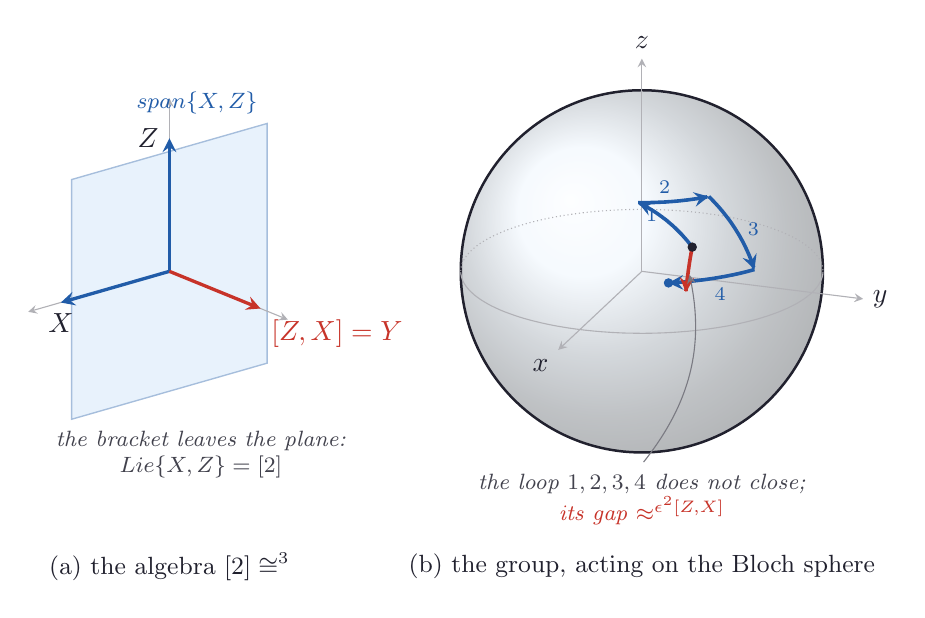
\begin{tikzpicture}[ink/.style={line width=0.9pt, ndInk}, faint/.style={line width=0.4pt, ndInk!35}, dashedink/.style={line width=0.5pt, ndInk!55, dash pattern=on 2.5pt off 2pt}, vec/.style={->, >=stealth, line width=1.2pt}, note/.style={font=\footnotesize\itshape, text=ndInk!85, align=center}, pointer/.style={->, >=stealth, line width=0.4pt, ndInk!60, shorten >=2pt, shorten <=1pt}, dot/.style={circle, fill=ndInk, inner sep=0pt, minimum size=3.4pt}, wash/.style={fill=ndSky, fill opacity=0.55}, every node/.style={text=ndInk}]
\definecolor{ndInk}{rgb}{0.13,0.13,0.18}
\definecolor{ndPaper}{rgb}{0.99,0.96,0.88}
\definecolor{ndSky}{rgb}{0.84,0.91,0.98}
\definecolor{ndRose}{rgb}{0.98,0.86,0.84}
\definecolor{ndBlue}{rgb}{0.13,0.36,0.66}
\definecolor{ndRed}{rgb}{0.78,0.20,0.16}
\definecolor{ndGold}{rgb}{0.88,0.62,0.10}
\definecolor{ndGreen}{rgb}{0.18,0.52,0.30}
\filldraw[wash, draw=ndBlue!40, line width=0.5pt] (1.241,-1.166) -- (-1.241,-1.878) -- (-1.241,1.166) -- (1.241,1.878) -- cycle;
\draw[faint, ->, >=stealth] (0.000,0.000) -- (-1.793,-0.514);
\draw[faint, ->, >=stealth] (0.000,0.000) -- (1.504,-0.613);
\draw[faint, ->, >=stealth] (0.000,0.000) -- (0.000,2.199);
\draw[vec, ndBlue] (0.000,0.000) -- (-1.379,-0.396) node[below] {$X$};
\draw[vec, ndBlue] (0.000,0.000) -- (0.000,1.691) node[left] {$Z$};
\draw[vec, ndRed] (0.000,0.000) -- (1.157,-0.472) node[below right, text=ndRed] {$[Z,X]=Y$};
\node[note, anchor=south east, text=ndBlue] at (1.241,1.878) {$\operatorname{span}\{X,Z\}$};
\node[note, anchor=north] (n) at (0.40,-1.90) {the bracket leaves the plane:\\$\operatorname{Lie}\{X,Z\}=\liesu[2]$};
\node[font=\small] at (0.00,-3.75) {(a) the algebra $\liesu[2]\cong\R^3$};
\shade[ball color=ndSky!70!white, opacity=0.45] (6.000,0.000) circle (2.300);
\draw[ink] (6.000,0.000) circle (2.300);
\draw[faint] (8.161,-0.269) -- (8.181,-0.250) -- (8.200,-0.230) -- (8.216,-0.210) -- (8.232,-0.190) -- (8.245,-0.170) -- (8.258,-0.150) -- (8.268,-0.130) -- (8.278,-0.109) -- (8.285,-0.089) -- (8.291,-0.069) -- (8.296,-0.048) -- (8.299,-0.027) -- (8.300,-0.007);
\draw[faint] (3.700,-0.014) -- (3.702,-0.034) -- (3.706,-0.055) -- (3.711,-0.075) -- (3.717,-0.096) -- (3.725,-0.116) -- (3.735,-0.137) -- (3.746,-0.157) -- (3.759,-0.177) -- (3.773,-0.197) -- (3.789,-0.217) -- (3.806,-0.237) -- (3.825,-0.256) -- (3.846,-0.275) -- (3.867,-0.295) -- (3.891,-0.314) -- (3.915,-0.332) -- (3.942,-0.351) -- (3.969,-0.369) -- (3.998,-0.387) -- (4.029,-0.405) -- (4.060,-0.423) -- (4.093,-0.440) -- (4.128,-0.457) -- (4.163,-0.473) -- (4.200,-0.490) -- (4.238,-0.506) -- (4.277,-0.521) -- (4.318,-0.536) -- (4.360,-0.551) -- (4.402,-0.566) -- (4.446,-0.580) -- (4.491,-0.594) -- (4.537,-0.607) -- (4.584,-0.620) -- (4.632,-0.632) -- (4.681,-0.644) -- (4.731,-0.656) -- (4.781,-0.667) -- (4.833,-0.678) -- (4.885,-0.688) -- (4.938,-0.698) -- (4.992,-0.707) -- (5.046,-0.716) -- (5.101,-0.724) -- (5.157,-0.732) -- (5.213,-0.739) -- (5.270,-0.746) -- (5.328,-0.752) -- (5.385,-0.758) -- (5.444,-0.763) -- (5.502,-0.768) -- (5.561,-0.772) -- (5.620,-0.776) -- (5.680,-0.779) -- (5.740,-0.782) -- (5.800,-0.784) -- (5.860,-0.785) -- (5.920,-0.786) -- (5.980,-0.787) -- (6.040,-0.787) -- (6.100,-0.786) -- (6.160,-0.785) -- (6.220,-0.783) -- (6.280,-0.781) -- (6.340,-0.778) -- (6.399,-0.775) -- (6.459,-0.771) -- (6.517,-0.766) -- (6.576,-0.762) -- (6.634,-0.756) -- (6.692,-0.750) -- (6.749,-0.744) -- (6.805,-0.737) -- (6.862,-0.729) -- (6.917,-0.721) -- (6.972,-0.713) -- (7.026,-0.704) -- (7.080,-0.695) -- (7.133,-0.685) -- (7.185,-0.674) -- (7.236,-0.663) -- (7.286,-0.652) -- (7.336,-0.640) -- (7.384,-0.628) -- (7.432,-0.616) -- (7.478,-0.603) -- (7.524,-0.589) -- (7.569,-0.575) -- (7.612,-0.561) -- (7.654,-0.546) -- (7.696,-0.531) -- (7.736,-0.516) -- (7.775,-0.500) -- (7.812,-0.484) -- (7.849,-0.468) -- (7.884,-0.451) -- (7.918,-0.434) -- (7.951,-0.417) -- (7.982,-0.399) -- (8.012,-0.381) -- (8.040,-0.363) -- (8.067,-0.345) -- (8.093,-0.326) -- (8.117,-0.307) -- (8.140,-0.288) -- (8.161,-0.269);
\draw[faint, densely dotted] (8.300,0.014) -- (8.298,0.034) -- (8.294,0.055) -- (8.289,0.075) -- (8.283,0.096) -- (8.275,0.116) -- (8.265,0.137) -- (8.254,0.157) -- (8.241,0.177) -- (8.227,0.197) -- (8.211,0.217) -- (8.194,0.237) -- (8.175,0.256) -- (8.154,0.275) -- (8.133,0.295) -- (8.109,0.314) -- (8.085,0.332) -- (8.058,0.351) -- (8.031,0.369) -- (8.002,0.387) -- (7.971,0.405) -- (7.940,0.423) -- (7.907,0.440) -- (7.872,0.457) -- (7.837,0.473) -- (7.800,0.490) -- (7.762,0.506) -- (7.723,0.521) -- (7.682,0.536) -- (7.640,0.551) -- (7.598,0.566) -- (7.554,0.580) -- (7.509,0.594) -- (7.463,0.607) -- (7.416,0.620) -- (7.368,0.632) -- (7.319,0.644) -- (7.269,0.656) -- (7.219,0.667) -- (7.167,0.678) -- (7.115,0.688) -- (7.062,0.698) -- (7.008,0.707) -- (6.954,0.716) -- (6.899,0.724) -- (6.843,0.732) -- (6.787,0.739) -- (6.730,0.746) -- (6.672,0.752) -- (6.615,0.758) -- (6.556,0.763) -- (6.498,0.768) -- (6.439,0.772) -- (6.380,0.776) -- (6.320,0.779) -- (6.260,0.782) -- (6.200,0.784) -- (6.140,0.785) -- (6.080,0.786) -- (6.020,0.787) -- (5.960,0.787) -- (5.900,0.786) -- (5.840,0.785) -- (5.780,0.783) -- (5.720,0.781) -- (5.660,0.778) -- (5.601,0.775) -- (5.541,0.771) -- (5.483,0.766) -- (5.424,0.762) -- (5.366,0.756) -- (5.308,0.750) -- (5.251,0.744) -- (5.195,0.737) -- (5.138,0.729) -- (5.083,0.721) -- (5.028,0.713) -- (4.974,0.704) -- (4.920,0.695) -- (4.867,0.685) -- (4.815,0.674) -- (4.764,0.663) -- (4.714,0.652) -- (4.664,0.640) -- (4.616,0.628) -- (4.568,0.616) -- (4.522,0.603) -- (4.476,0.589) -- (4.431,0.575) -- (4.388,0.561) -- (4.346,0.546) -- (4.304,0.531) -- (4.264,0.516) -- (4.225,0.500) -- (4.188,0.484) -- (4.151,0.468) -- (4.116,0.451) -- (4.082,0.434) -- (4.049,0.417) -- (4.018,0.399) -- (3.988,0.381) -- (3.960,0.363) -- (3.933,0.345) -- (3.907,0.326) -- (3.883,0.307) -- (3.860,0.288) -- (3.839,0.269) -- (3.819,0.250) -- (3.800,0.230) -- (3.784,0.210) -- (3.768,0.190) -- (3.755,0.170) -- (3.742,0.150) -- (3.732,0.130) -- (3.722,0.109) -- (3.715,0.089) -- (3.709,0.069) -- (3.704,0.048) -- (3.701,0.027) -- (3.700,0.007);
\draw[faint, ->, >=stealth] (6.000,0.000) -- (6.000,2.702) node[above] {$z$};
\draw[faint, ->, >=stealth] (6.000,0.000) -- (4.938,-0.998) node[below left] {$x$};
\draw[faint, ->, >=stealth] (6.000,0.000) -- (8.810,-0.350) node[right] {$y$};
\draw[->, >=stealth, line width=1.3pt, ndBlue] (6.640,0.308) -- (6.626,0.326) -- (6.612,0.344) -- (6.598,0.361) -- (6.584,0.379) -- (6.570,0.396) -- (6.555,0.413) -- (6.540,0.430) -- (6.525,0.447) -- (6.510,0.464) -- (6.495,0.480) -- (6.479,0.496) -- (6.463,0.512) -- (6.447,0.528) -- (6.431,0.544) -- (6.415,0.559) -- (6.398,0.575) -- (6.381,0.590) -- (6.364,0.604) -- (6.347,0.619) -- (6.330,0.633) -- (6.313,0.648) -- (6.295,0.662) -- (6.277,0.675) -- (6.259,0.689) -- (6.241,0.702) -- (6.223,0.715) -- (6.205,0.728) -- (6.186,0.741) -- (6.168,0.753) -- (6.149,0.765) -- (6.130,0.777) -- (6.111,0.788) -- (6.092,0.800) -- (6.072,0.811) -- (6.053,0.822) -- (6.033,0.832) -- (6.014,0.843) -- (5.994,0.853) -- (5.974,0.863) -- (5.954,0.872);
\node[font=\scriptsize, text=ndBlue] at (6.125,0.714) {1};
\draw[->, >=stealth, line width=1.3pt, ndBlue] (5.954,0.872) -- (5.978,0.872) -- (6.001,0.872) -- (6.024,0.872) -- (6.048,0.872) -- (6.071,0.873) -- (6.095,0.873) -- (6.118,0.874) -- (6.141,0.874) -- (6.165,0.875) -- (6.188,0.876) -- (6.211,0.877) -- (6.234,0.878) -- (6.257,0.879) -- (6.281,0.880) -- (6.304,0.881) -- (6.327,0.883) -- (6.350,0.885) -- (6.372,0.886) -- (6.395,0.888) -- (6.418,0.890) -- (6.441,0.892) -- (6.463,0.894) -- (6.486,0.896) -- (6.508,0.899) -- (6.530,0.901) -- (6.552,0.904) -- (6.574,0.906) -- (6.596,0.909) -- (6.618,0.912) -- (6.640,0.915) -- (6.662,0.918) -- (6.683,0.921) -- (6.705,0.924) -- (6.726,0.928) -- (6.747,0.931) -- (6.768,0.935) -- (6.789,0.938) -- (6.809,0.942) -- (6.830,0.946) -- (6.850,0.950);
\node[font=\scriptsize, text=ndBlue] at (6.291,1.069) {2};
\draw[->, >=stealth, line width=1.3pt, ndBlue] (6.850,0.950) -- (6.870,0.931) -- (6.890,0.911) -- (6.909,0.891) -- (6.928,0.871) -- (6.947,0.850) -- (6.966,0.830) -- (6.984,0.809) -- (7.002,0.788) -- (7.020,0.767) -- (7.038,0.745) -- (7.055,0.723) -- (7.072,0.701) -- (7.089,0.679) -- (7.106,0.657) -- (7.122,0.635) -- (7.138,0.612) -- (7.154,0.589) -- (7.169,0.566) -- (7.184,0.543) -- (7.199,0.519) -- (7.213,0.496) -- (7.228,0.472) -- (7.242,0.448) -- (7.255,0.424) -- (7.269,0.400) -- (7.282,0.376) -- (7.294,0.351) -- (7.307,0.327) -- (7.319,0.302) -- (7.330,0.277) -- (7.342,0.252) -- (7.353,0.227) -- (7.364,0.202) -- (7.374,0.177) -- (7.384,0.152) -- (7.394,0.126) -- (7.403,0.101) -- (7.412,0.075) -- (7.421,0.049) -- (7.430,0.023);
\node[font=\scriptsize, text=ndBlue] at (7.418,0.534) {3};
\draw[->, >=stealth, line width=1.3pt, ndBlue] (7.430,0.023) -- (7.406,0.017) -- (7.383,0.010) -- (7.359,0.004) -- (7.335,-0.003) -- (7.310,-0.009) -- (7.286,-0.015) -- (7.261,-0.021) -- (7.236,-0.027) -- (7.211,-0.033) -- (7.185,-0.038) -- (7.159,-0.044) -- (7.133,-0.049) -- (7.107,-0.054) -- (7.081,-0.059) -- (7.054,-0.065) -- (7.027,-0.069) -- (7.000,-0.074) -- (6.973,-0.079) -- (6.946,-0.083) -- (6.918,-0.088) -- (6.891,-0.092) -- (6.863,-0.096) -- (6.835,-0.100) -- (6.806,-0.104) -- (6.778,-0.108) -- (6.750,-0.111) -- (6.721,-0.115) -- (6.692,-0.118) -- (6.663,-0.121) -- (6.634,-0.124) -- (6.605,-0.127) -- (6.576,-0.130) -- (6.546,-0.133) -- (6.517,-0.135) -- (6.487,-0.137) -- (6.458,-0.140) -- (6.428,-0.142) -- (6.398,-0.144) -- (6.368,-0.146) -- (6.338,-0.147);
\node[font=\scriptsize, text=ndBlue] at (6.995,-0.294) {4};
\draw[->, >=stealth, line width=1.3pt, ndRed] (6.640,0.308) -- (6.637,0.294) -- (6.634,0.280) -- (6.632,0.266) -- (6.629,0.252) -- (6.627,0.238) -- (6.624,0.224) -- (6.622,0.209) -- (6.619,0.195) -- (6.617,0.181) -- (6.614,0.167) -- (6.612,0.153) -- (6.610,0.138) -- (6.607,0.124) -- (6.605,0.110) -- (6.603,0.096) -- (6.601,0.081) -- (6.599,0.067) -- (6.597,0.053) -- (6.595,0.038) -- (6.592,0.024) -- (6.590,0.010) -- (6.589,-0.005) -- (6.587,-0.019) -- (6.585,-0.034) -- (6.583,-0.048) -- (6.581,-0.062) -- (6.579,-0.077) -- (6.577,-0.091) -- (6.576,-0.106) -- (6.574,-0.120) -- (6.572,-0.134) -- (6.571,-0.149) -- (6.569,-0.163) -- (6.568,-0.178) -- (6.566,-0.192) -- (6.565,-0.206) -- (6.563,-0.221) -- (6.562,-0.235) -- (6.560,-0.250) -- (6.559,-0.264);
\node[dot] at (6.640,0.308) {};
\node[dot, fill=ndBlue] at (6.338,-0.147) {};
\node[note, anchor=north] (m) at (6.00,-2.45) {the loop $1,2,3,4$ does not close;\\\textcolor{ndRed}{its gap $\approx\ee^{\epsilon^2[Z,X]}$}};
\draw[pointer] (m.north) to[bend right=25] (6.592,0.024);
\node[font=\small] at (6.00,-3.75) {(b) the group, acting on the Bloch sphere};
\end{tikzpicture}
}\end{center}
Switching $X$, $Z$ on and off in a loop moves along $\comm{Z}{X}$: brackets are reachable directions.}
\end{frame}

\section{The Schr\"odinger equation and the propagator}\label{sec:ch02:schrodinger}

\begin{frame}\ft{Time evolution}
\ona{We now allow the Hamiltonian $H(t)\in\Herm[\Hil]$ to depend on time, as it does when we switch control fields on and off. The Schr\"odinger equation of Section~\ref{sec:ch02:qm} becomes (with $\hbar=1$)}
\begin{equation}\label{eq:schrodinger}
    \imath\,\dd{t}\ket{\psi(t)} = H(t)\ket{\psi(t)}, \qquad \ket{\psi(0)}=\ket{\psi_0}.
\end{equation}
\ona{The norm of $\ket\psi$ is conserved, $\braket{\psi(t)|\psi(t)}=1$, so the state moves on the unit sphere of $\Hil$. Since \eqref{eq:schrodinger} is linear, its solution is $\ket{\psi(t)}=U(t)\ket{\psi_0}$ with the \emph{propagator} $U(t)$ solving}
\onp{Norm is conserved. Linear, so $\ket{\psi(t)}=U(t)\ket{\psi_0}$ with the \alert{propagator}}
\begin{equation}\label{eq:propagator-eq}
    \dot U(t) = -\imath H(t)\,U(t),\qquad U(0)=\Id.
\end{equation}
\begin{propn}\label{prop:unitary}
The solution of \eqref{eq:propagator-eq} is unitary for all $t$. If $H(t)\equiv H$ then $U(t)=\ee^{-\imath Ht}$. In general $U(t)=\Texp\big(-\imath\int_0^t H(s)\,\mathrm{d}s\big)$, the \emph{time-ordered exponential} (Dyson series), which is \emph{not} $\exp(-\imath\int_0^t H)$ unless the $H(s)$ commute.
\end{propn}
\ona{Informally, the time-ordered exponential is the limit of the products $\ee^{-\imath H(t_L)\Delta t}\cdots\ee^{-\imath H(t_1)\Delta t}$ over finer and finer time grids, with later times on the left; for piecewise-constant $H$ it is exactly such a product, see \eqref{eq:pwc}.}
\ona{\begin{pf}
$\dd{t}(U^\dagger U)=U^\dagger(\imath H)U+U^\dagger(-\imath H)U=0$, so $U^\dagger U\equiv\Id$. For constant $H$ differentiate $\ee^{-\imath Ht}$. For the general case, iterate the integral form $U(t)=\Id-\imath\int_0^tH(s)U(s)\,\mathrm{d}s$; the resulting series of time-ordered integrals is the Dyson series
\[
U(t)=\Id+\sum_{k\ge1}(-\imath)^k\int_{t>s_1>\dots>s_k>0}H(s_1)\cdots H(s_k)\,\mathrm{d}s_1\cdots\mathrm{d}s_k .
\]
\end{pf}}
\ona{\endgraf\medskip\noindent\emph{What ``solution'' means.} With admissible controls $u\in L^\infty$, the Hamiltonian $t\mapsto H(u(t))$ is bounded and measurable but may jump, so $\dot U(t)$ need not exist at every $t$. The equation \eqref{eq:propagator-eq} is therefore understood in the sense of Carath\'eodory: $U$ is absolutely continuous and satisfies the integral equation $U(t)=\Id-\imath\int_0^tH(s)U(s)\,\mathrm ds$, hence \eqref{eq:propagator-eq} at almost every $t$. Such a solution exists and is unique on every interval $[0,T]$: the right-hand side is linear in $U$ with an integrable coefficient, and the Picard iteration, which is exactly the Dyson series, converges. The unitarity argument in the proof needs one extra remark. The function $U^\dagger U$ is absolutely continuous, and an absolutely continuous function whose derivative vanishes almost everywhere is constant. For functions that are merely differentiable almost everywhere this conclusion is false; the Cantor function is the standard counterexample.}
\end{frame}

\begin{frame}\ft{Dyson versus Magnus}
\ona{Both series are exact when summed to all orders; in practice one truncates them, and they behave very differently when truncated. The Magnus expansion re-sums the Dyson series into a single exponential.}
\begin{propn}[Magnus expansion]\label{prop:ch02:magnus}
If $\int_0^t\opnorm{H(s)}\,\mathrm{d}s<\pi$, where $\opnorm{H}$ is the operator norm (the largest $\abs{\text{eigenvalue}}$ of $H$), then $U(t)=\ee^{\Omega(t)}$ with $\Omega=\sum_{k\ge1}\Omega_k$,
\[
\Omega_1(t)=-\imath\!\int_0^t\! H(s)\,\mathrm{d}s,\qquad
\Omega_2(t)=-\tfrac12\!\int_0^t\!\!\int_0^{s}\comm{H(s)}{H(s')}\,\mathrm{d}s'\,\mathrm{d}s,
\]
and in general $\Omega_k$ is a $k$-fold integral of $(k-1)$-fold nested commutators of the $-\imath H(s_i)$. Each $\Omega_k$ is anti-Hermitian, so every truncation $\ee^{\Omega_1+\dots+\Omega_K}$ is \emph{exactly unitary}.
\end{propn}
\ona{\begin{pf}
Expanding $\ee^{\Omega}$ and matching terms of equal order in $H$ with the Dyson series gives $\Omega_1$ and $\Omega_2$; the convergence condition is due to \citet{moan2008convergence}, see also the review of \citet{blanes2009magnus}. Since $-\imath H(s)\in\lieu[N]$ and $\lieu[N]$ is closed under real linear combinations and commutators, every $\Omega_k$ lies in $\lieu[N]$, and $\ee^{X}\in\Un[N]$ for $X\in\lieu[N]$.
\end{pf}}
\ona{The norm in the hypothesis matters: it is the operator norm, which can be smaller than the Hilbert--Schmidt norm $\norm{\cdot}$ used elsewhere in this \chap{} by a factor up to $\sqrt N$. The condition is sufficient, not necessary, and the bound $\pi$ has a simple meaning. The series tries to produce a logarithm of $U(t)$, and logarithms of unitaries are unique only while no eigenvalue has wound half-way round the circle: in $\Un[1]$, $\ee^{-\imath\theta}=\ee^{\Omega}$ determines $\Omega=-\imath\theta$ uniquely among small exponents only for $\abs\theta<\pi$.}
\ona{A truncated Dyson series, by contrast, is a polynomial in the $H(s)$ and is not unitary: the norm of the propagated state drifts away from $1$, and the error accumulates over long times. Truncated Magnus keeps the approximation on the group $\Un[N]$, so its error is a wrong unitary rather than a loss of probability. For this reason Magnus-type integrators are preferred for propagating quantum states; the exponential midpoint rule $\ee^{-\imath H(t+\Delta t/2)\Delta t}$ is the lowest-order one. The first-order term $\Omega_1$ is the \emph{average Hamiltonian} of pulse design, and $\Omega_2$ is its leading correction. For piecewise-constant $H$ each piece has $\Omega=\Omega_1$ exactly, which gives the product formula \eqref{eq:pwc} below.}
\onp{\begin{itemize}
    \item Truncated Dyson: a polynomial in $H$, \alert{not unitary}; norm drifts.
    \item Truncated Magnus: stays on $\Un[N]$ (\alert{unitary} at every order); basis of exponential integrators.
    \item $\Omega_1$ = average Hamiltonian; piecewise-constant $H$: $\Omega=\Omega_1$ on each piece.
\end{itemize}}
\end{frame}

\begin{frame}\ft{Truncated Dyson leaves the group}
\ona{The difference between the two expansions is already visible in the smallest unitary group, $\Un[1]$, the unit circle in $\C$ (Figure~\ref{fig:ch02:magnus}). Take $H=1$, so that $U(t)=\ee^{-\imath\theta}$ with $\theta=t$. The first-order Dyson truncation $D_1=1-\imath\theta$ moves along the tangent line at $1$, i.e.\ in the direction of the Lie algebra $\imath\R$, and $|D_1|=\sqrt{1+\theta^2}>1$. Higher truncations $D_K=\sum_{k\le K}(-\imath\theta)^k/k!$ come closer to the circle but do not stay on it: $\abs{D_K(\theta)}=1$ holds only at isolated values of $\theta$. For instance $\abs{D_3(\theta)}^2=1-\theta^4/12+\theta^6/36$, which equals $1$ at $\theta=\sqrt3$, so the curve $D_3$ crosses the circle there, beyond the range shown. Every Magnus truncation is the exponential of an element of $\imath\R$ and so lies on the circle. Here all $H(t)$ commute, so $\Omega_1$ is already exact; in general a truncated Magnus series lands at a slightly wrong point, but still on the group.}
\ona{\begin{figure}[h]\centering
\resizebox{0.85\linewidth}{!}{% Generated by code/needham.py -- do not edit by hand.
\definecolor{qocA}{rgb}{0.00,0.45,0.70}
\definecolor{qocB}{rgb}{0.90,0.60,0.00}
\definecolor{qocC}{rgb}{0.00,0.62,0.45}
\definecolor{qocD}{rgb}{0.80,0.40,0.00}
\definecolor{qocE}{rgb}{0.80,0.60,0.70}
\definecolor{qocF}{rgb}{0.35,0.70,0.90}
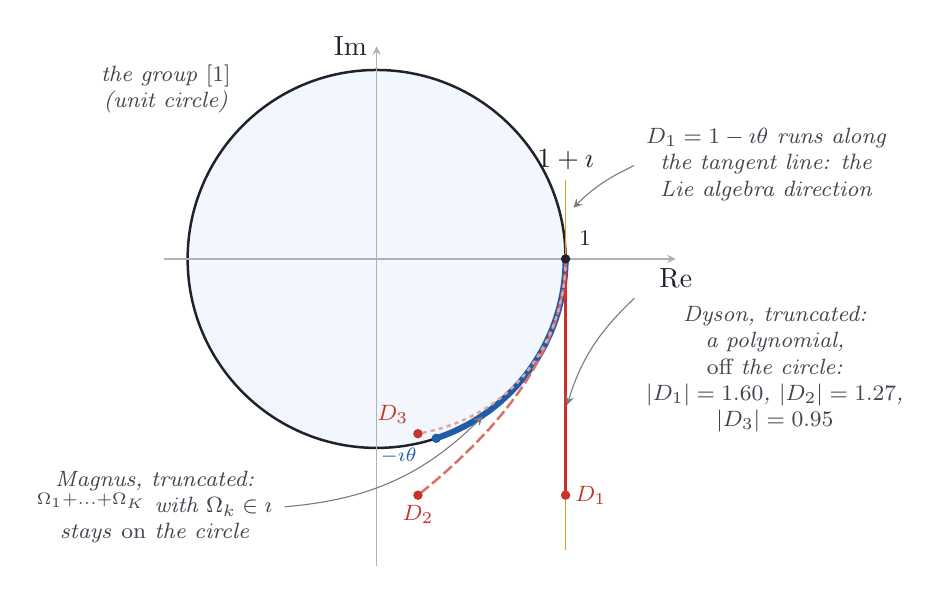
\begin{tikzpicture}[ink/.style={line width=0.9pt, ndInk}, faint/.style={line width=0.4pt, ndInk!35}, dashedink/.style={line width=0.5pt, ndInk!55, dash pattern=on 2.5pt off 2pt}, vec/.style={->, >=stealth, line width=1.2pt}, note/.style={font=\footnotesize\itshape, text=ndInk!85, align=center}, pointer/.style={->, >=stealth, line width=0.4pt, ndInk!60, shorten >=2pt, shorten <=1pt}, dot/.style={circle, fill=ndInk, inner sep=0pt, minimum size=3.4pt}, wash/.style={fill=ndSky, fill opacity=0.55}, every node/.style={text=ndInk}]
\definecolor{ndInk}{rgb}{0.13,0.13,0.18}
\definecolor{ndPaper}{rgb}{0.99,0.96,0.88}
\definecolor{ndSky}{rgb}{0.84,0.91,0.98}
\definecolor{ndRose}{rgb}{0.98,0.86,0.84}
\definecolor{ndBlue}{rgb}{0.13,0.36,0.66}
\definecolor{ndRed}{rgb}{0.78,0.20,0.16}
\definecolor{ndGold}{rgb}{0.88,0.62,0.10}
\definecolor{ndGreen}{rgb}{0.18,0.52,0.30}
\fill[ndSky, fill opacity=0.35] (0,0) circle (2.400);
\draw[ink] (0,0) circle (2.400);
\draw[faint, ->, >=stealth] (-2.70,0) -- (3.80,0) node[below] {$\mathrm{Re}$};
\draw[faint, ->, >=stealth] (0,-3.90) -- (0,2.70) node[left] {$\mathrm{Im}$};
\draw[line width=0.6pt, ndGold] (2.400,-3.700) -- (2.400,1.000) node[above] {$1+\imath\R$};
\draw[line width=2.2pt, ndBlue] (2.400,0.000) -- (2.400,-0.038) -- (2.399,-0.076) -- (2.397,-0.114) -- (2.395,-0.152) -- (2.392,-0.190) -- (2.389,-0.228) -- (2.385,-0.265) -- (2.381,-0.303) -- (2.376,-0.341) -- (2.370,-0.378) -- (2.364,-0.416) -- (2.357,-0.453) -- (2.349,-0.490) -- (2.341,-0.527) -- (2.333,-0.564) -- (2.323,-0.601) -- (2.314,-0.638) -- (2.303,-0.674) -- (2.292,-0.711) -- (2.281,-0.747) -- (2.269,-0.783) -- (2.256,-0.819) -- (2.243,-0.854) -- (2.229,-0.890) -- (2.215,-0.925) -- (2.200,-0.960) -- (2.184,-0.994) -- (2.168,-1.029) -- (2.152,-1.063) -- (2.135,-1.097) -- (2.117,-1.131) -- (2.099,-1.164) -- (2.080,-1.197) -- (2.061,-1.230) -- (2.041,-1.262) -- (2.021,-1.294) -- (2.000,-1.326) -- (1.979,-1.358) -- (1.957,-1.389) -- (1.935,-1.420) -- (1.912,-1.450) -- (1.889,-1.480) -- (1.866,-1.510) -- (1.841,-1.539) -- (1.817,-1.568) -- (1.792,-1.597) -- (1.766,-1.625) -- (1.740,-1.653) -- (1.714,-1.680) -- (1.687,-1.707) -- (1.660,-1.733) -- (1.632,-1.759) -- (1.604,-1.785) -- (1.576,-1.810) -- (1.547,-1.835) -- (1.518,-1.859) -- (1.488,-1.883) -- (1.458,-1.906) -- (1.428,-1.929) -- (1.397,-1.951) -- (1.366,-1.973) -- (1.335,-1.995) -- (1.303,-2.015) -- (1.271,-2.036) -- (1.239,-2.056) -- (1.206,-2.075) -- (1.173,-2.094) -- (1.140,-2.112) -- (1.106,-2.130) -- (1.072,-2.147) -- (1.038,-2.164) -- (1.004,-2.180) -- (0.969,-2.196) -- (0.934,-2.211) -- (0.899,-2.225) -- (0.864,-2.239) -- (0.828,-2.252) -- (0.793,-2.265) -- (0.757,-2.278);
\draw[line width=0.9pt, ndRed] (2.400,0.000) -- (2.400,-0.038) -- (2.400,-0.076) -- (2.400,-0.114) -- (2.400,-0.152) -- (2.400,-0.190) -- (2.400,-0.228) -- (2.400,-0.266) -- (2.400,-0.304) -- (2.400,-0.342) -- (2.400,-0.380) -- (2.400,-0.418) -- (2.400,-0.456) -- (2.400,-0.494) -- (2.400,-0.532) -- (2.400,-0.570) -- (2.400,-0.608) -- (2.400,-0.646) -- (2.400,-0.684) -- (2.400,-0.722) -- (2.400,-0.759) -- (2.400,-0.797) -- (2.400,-0.835) -- (2.400,-0.873) -- (2.400,-0.911) -- (2.400,-0.949) -- (2.400,-0.987) -- (2.400,-1.025) -- (2.400,-1.063) -- (2.400,-1.101) -- (2.400,-1.139) -- (2.400,-1.177) -- (2.400,-1.215) -- (2.400,-1.253) -- (2.400,-1.291) -- (2.400,-1.329) -- (2.400,-1.367) -- (2.400,-1.405) -- (2.400,-1.443) -- (2.400,-1.481) -- (2.400,-1.519) -- (2.400,-1.557) -- (2.400,-1.595) -- (2.400,-1.633) -- (2.400,-1.671) -- (2.400,-1.709) -- (2.400,-1.747) -- (2.400,-1.785) -- (2.400,-1.823) -- (2.400,-1.861) -- (2.400,-1.899) -- (2.400,-1.937) -- (2.400,-1.975) -- (2.400,-2.013) -- (2.400,-2.051) -- (2.400,-2.089) -- (2.400,-2.127) -- (2.400,-2.165) -- (2.400,-2.203) -- (2.400,-2.241) -- (2.400,-2.278) -- (2.400,-2.316) -- (2.400,-2.354) -- (2.400,-2.392) -- (2.400,-2.430) -- (2.400,-2.468) -- (2.400,-2.506) -- (2.400,-2.544) -- (2.400,-2.582) -- (2.400,-2.620) -- (2.400,-2.658) -- (2.400,-2.696) -- (2.400,-2.734) -- (2.400,-2.772) -- (2.400,-2.810) -- (2.400,-2.848) -- (2.400,-2.886) -- (2.400,-2.924) -- (2.400,-2.962) -- (2.400,-3.000);
\node[dot, fill=ndRed] at (2.400,-3.000) {};
\node[right, text=ndRed, font=\footnotesize] at (2.400,-3.000) {$D_1$};
\draw[line width=0.9pt, ndRed!70, dash pattern=on 4pt off 1.5pt] (2.400,0.000) -- (2.400,-0.038) -- (2.399,-0.076) -- (2.397,-0.114) -- (2.395,-0.152) -- (2.392,-0.190) -- (2.389,-0.228) -- (2.385,-0.266) -- (2.381,-0.304) -- (2.376,-0.342) -- (2.370,-0.380) -- (2.364,-0.418) -- (2.357,-0.456) -- (2.349,-0.494) -- (2.341,-0.532) -- (2.332,-0.570) -- (2.323,-0.608) -- (2.313,-0.646) -- (2.303,-0.684) -- (2.292,-0.722) -- (2.280,-0.759) -- (2.268,-0.797) -- (2.255,-0.835) -- (2.241,-0.873) -- (2.227,-0.911) -- (2.212,-0.949) -- (2.197,-0.987) -- (2.181,-1.025) -- (2.164,-1.063) -- (2.147,-1.101) -- (2.130,-1.139) -- (2.111,-1.177) -- (2.092,-1.215) -- (2.073,-1.253) -- (2.053,-1.291) -- (2.032,-1.329) -- (2.011,-1.367) -- (1.989,-1.405) -- (1.966,-1.443) -- (1.943,-1.481) -- (1.919,-1.519) -- (1.895,-1.557) -- (1.870,-1.595) -- (1.845,-1.633) -- (1.818,-1.671) -- (1.792,-1.709) -- (1.764,-1.747) -- (1.736,-1.785) -- (1.708,-1.823) -- (1.679,-1.861) -- (1.649,-1.899) -- (1.619,-1.937) -- (1.588,-1.975) -- (1.556,-2.013) -- (1.524,-2.051) -- (1.491,-2.089) -- (1.458,-2.127) -- (1.424,-2.165) -- (1.389,-2.203) -- (1.354,-2.241) -- (1.318,-2.278) -- (1.282,-2.316) -- (1.245,-2.354) -- (1.208,-2.392) -- (1.169,-2.430) -- (1.131,-2.468) -- (1.091,-2.506) -- (1.051,-2.544) -- (1.011,-2.582) -- (0.970,-2.620) -- (0.928,-2.658) -- (0.886,-2.696) -- (0.843,-2.734) -- (0.799,-2.772) -- (0.755,-2.810) -- (0.710,-2.848) -- (0.665,-2.886) -- (0.619,-2.924) -- (0.572,-2.962) -- (0.525,-3.000);
\node[dot, fill=ndRed] at (0.525,-3.000) {};
\node[below, text=ndRed, font=\footnotesize] at (0.525,-3.000) {$D_2$};
\draw[line width=0.9pt, ndRed!45, dash pattern=on 1.5pt off 1.5pt] (2.400,0.000) -- (2.400,-0.038) -- (2.399,-0.076) -- (2.397,-0.114) -- (2.395,-0.152) -- (2.392,-0.190) -- (2.389,-0.228) -- (2.385,-0.265) -- (2.381,-0.303) -- (2.376,-0.341) -- (2.370,-0.378) -- (2.364,-0.416) -- (2.357,-0.453) -- (2.349,-0.490) -- (2.341,-0.527) -- (2.332,-0.564) -- (2.323,-0.601) -- (2.313,-0.638) -- (2.303,-0.674) -- (2.292,-0.711) -- (2.280,-0.747) -- (2.268,-0.783) -- (2.255,-0.819) -- (2.241,-0.854) -- (2.227,-0.889) -- (2.212,-0.925) -- (2.197,-0.959) -- (2.181,-0.994) -- (2.164,-1.029) -- (2.147,-1.063) -- (2.130,-1.096) -- (2.111,-1.130) -- (2.092,-1.163) -- (2.073,-1.196) -- (2.053,-1.229) -- (2.032,-1.261) -- (2.011,-1.293) -- (1.989,-1.325) -- (1.966,-1.356) -- (1.943,-1.387) -- (1.919,-1.418) -- (1.895,-1.448) -- (1.870,-1.478) -- (1.845,-1.507) -- (1.818,-1.536) -- (1.792,-1.564) -- (1.764,-1.593) -- (1.736,-1.620) -- (1.708,-1.648) -- (1.679,-1.674) -- (1.649,-1.701) -- (1.619,-1.727) -- (1.588,-1.752) -- (1.556,-1.777) -- (1.524,-1.801) -- (1.491,-1.825) -- (1.458,-1.848) -- (1.424,-1.871) -- (1.389,-1.893) -- (1.354,-1.915) -- (1.318,-1.936) -- (1.282,-1.957) -- (1.245,-1.977) -- (1.208,-1.996) -- (1.169,-2.015) -- (1.131,-2.033) -- (1.091,-2.051) -- (1.051,-2.068) -- (1.011,-2.084) -- (0.970,-2.100) -- (0.928,-2.115) -- (0.886,-2.129) -- (0.843,-2.143) -- (0.799,-2.156) -- (0.755,-2.168) -- (0.710,-2.180) -- (0.665,-2.190) -- (0.619,-2.201) -- (0.572,-2.210) -- (0.525,-2.219);
\node[dot, fill=ndRed] at (0.525,-2.219) {};
\node[above left, text=ndRed, font=\footnotesize] at (0.525,-2.219) {$D_3$};
\node[dot, fill=ndBlue] at (0.757,-2.278) {};
\node[below left, text=ndBlue, xshift=-3pt] at (0.757,-2.278) {$\ee^{-\imath\theta}$};
\node[dot, label={[font=\footnotesize]above right:$1$}] at (2.400,0) {};
\node[note, anchor=west] (d) at (3.30,-1.40) {Dyson, truncated:\\ a polynomial,\\\emph{off} the circle:\\ $|D_1|=1.60$, $|D_2|=1.27$,\\ $|D_3|=0.95$};
\draw[pointer] (d.north west) to[bend right=15] (2.400,-1.920);
\node[note, anchor=east] (m) at (-1.20,-3.15) {Magnus, truncated:\\$\ee^{\Omega_1+\dots+\Omega_K}$ with $\Omega_k\in\imath\R$\\ stays \emph{on} the circle};
\draw[pointer] (m.east) to[bend right=20] (1.396,-1.952);
\node[note, anchor=south east] at (-1.73,1.73) {the group $\Un[1]$\\ (unit circle)};
\node[note, anchor=west] (t) at (3.30,1.20) {$D_1=1-\imath\theta$ runs along\\ the tangent line: the\\ Lie algebra direction};
\draw[pointer] (t.west) to[bend right=10] (2.450,0.600);
\end{tikzpicture}
}
\caption{The group $\Un[1]$ and $H=1$: the exact propagator $\ee^{-\imath\theta}$ (blue) and the Dyson truncations $D_1,D_2,D_3$ (red), shown up to $\theta=1.25$. The Dyson truncations leave the circle. Generated by \texttt{code/ch02\_magnus.py}.}\label{fig:ch02:magnus}
\end{figure}}
\onp{\begin{center}\resizebox{!}{0.64\textheight}{% Generated by code/needham.py -- do not edit by hand.
\definecolor{qocA}{rgb}{0.00,0.45,0.70}
\definecolor{qocB}{rgb}{0.90,0.60,0.00}
\definecolor{qocC}{rgb}{0.00,0.62,0.45}
\definecolor{qocD}{rgb}{0.80,0.40,0.00}
\definecolor{qocE}{rgb}{0.80,0.60,0.70}
\definecolor{qocF}{rgb}{0.35,0.70,0.90}
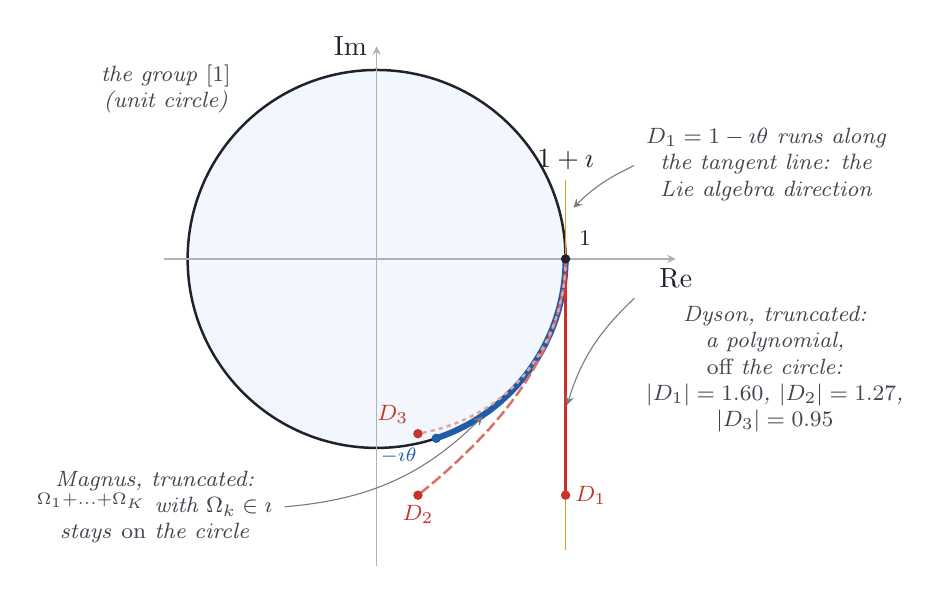
\begin{tikzpicture}[ink/.style={line width=0.9pt, ndInk}, faint/.style={line width=0.4pt, ndInk!35}, dashedink/.style={line width=0.5pt, ndInk!55, dash pattern=on 2.5pt off 2pt}, vec/.style={->, >=stealth, line width=1.2pt}, note/.style={font=\footnotesize\itshape, text=ndInk!85, align=center}, pointer/.style={->, >=stealth, line width=0.4pt, ndInk!60, shorten >=2pt, shorten <=1pt}, dot/.style={circle, fill=ndInk, inner sep=0pt, minimum size=3.4pt}, wash/.style={fill=ndSky, fill opacity=0.55}, every node/.style={text=ndInk}]
\definecolor{ndInk}{rgb}{0.13,0.13,0.18}
\definecolor{ndPaper}{rgb}{0.99,0.96,0.88}
\definecolor{ndSky}{rgb}{0.84,0.91,0.98}
\definecolor{ndRose}{rgb}{0.98,0.86,0.84}
\definecolor{ndBlue}{rgb}{0.13,0.36,0.66}
\definecolor{ndRed}{rgb}{0.78,0.20,0.16}
\definecolor{ndGold}{rgb}{0.88,0.62,0.10}
\definecolor{ndGreen}{rgb}{0.18,0.52,0.30}
\fill[ndSky, fill opacity=0.35] (0,0) circle (2.400);
\draw[ink] (0,0) circle (2.400);
\draw[faint, ->, >=stealth] (-2.70,0) -- (3.80,0) node[below] {$\mathrm{Re}$};
\draw[faint, ->, >=stealth] (0,-3.90) -- (0,2.70) node[left] {$\mathrm{Im}$};
\draw[line width=0.6pt, ndGold] (2.400,-3.700) -- (2.400,1.000) node[above] {$1+\imath\R$};
\draw[line width=2.2pt, ndBlue] (2.400,0.000) -- (2.400,-0.038) -- (2.399,-0.076) -- (2.397,-0.114) -- (2.395,-0.152) -- (2.392,-0.190) -- (2.389,-0.228) -- (2.385,-0.265) -- (2.381,-0.303) -- (2.376,-0.341) -- (2.370,-0.378) -- (2.364,-0.416) -- (2.357,-0.453) -- (2.349,-0.490) -- (2.341,-0.527) -- (2.333,-0.564) -- (2.323,-0.601) -- (2.314,-0.638) -- (2.303,-0.674) -- (2.292,-0.711) -- (2.281,-0.747) -- (2.269,-0.783) -- (2.256,-0.819) -- (2.243,-0.854) -- (2.229,-0.890) -- (2.215,-0.925) -- (2.200,-0.960) -- (2.184,-0.994) -- (2.168,-1.029) -- (2.152,-1.063) -- (2.135,-1.097) -- (2.117,-1.131) -- (2.099,-1.164) -- (2.080,-1.197) -- (2.061,-1.230) -- (2.041,-1.262) -- (2.021,-1.294) -- (2.000,-1.326) -- (1.979,-1.358) -- (1.957,-1.389) -- (1.935,-1.420) -- (1.912,-1.450) -- (1.889,-1.480) -- (1.866,-1.510) -- (1.841,-1.539) -- (1.817,-1.568) -- (1.792,-1.597) -- (1.766,-1.625) -- (1.740,-1.653) -- (1.714,-1.680) -- (1.687,-1.707) -- (1.660,-1.733) -- (1.632,-1.759) -- (1.604,-1.785) -- (1.576,-1.810) -- (1.547,-1.835) -- (1.518,-1.859) -- (1.488,-1.883) -- (1.458,-1.906) -- (1.428,-1.929) -- (1.397,-1.951) -- (1.366,-1.973) -- (1.335,-1.995) -- (1.303,-2.015) -- (1.271,-2.036) -- (1.239,-2.056) -- (1.206,-2.075) -- (1.173,-2.094) -- (1.140,-2.112) -- (1.106,-2.130) -- (1.072,-2.147) -- (1.038,-2.164) -- (1.004,-2.180) -- (0.969,-2.196) -- (0.934,-2.211) -- (0.899,-2.225) -- (0.864,-2.239) -- (0.828,-2.252) -- (0.793,-2.265) -- (0.757,-2.278);
\draw[line width=0.9pt, ndRed] (2.400,0.000) -- (2.400,-0.038) -- (2.400,-0.076) -- (2.400,-0.114) -- (2.400,-0.152) -- (2.400,-0.190) -- (2.400,-0.228) -- (2.400,-0.266) -- (2.400,-0.304) -- (2.400,-0.342) -- (2.400,-0.380) -- (2.400,-0.418) -- (2.400,-0.456) -- (2.400,-0.494) -- (2.400,-0.532) -- (2.400,-0.570) -- (2.400,-0.608) -- (2.400,-0.646) -- (2.400,-0.684) -- (2.400,-0.722) -- (2.400,-0.759) -- (2.400,-0.797) -- (2.400,-0.835) -- (2.400,-0.873) -- (2.400,-0.911) -- (2.400,-0.949) -- (2.400,-0.987) -- (2.400,-1.025) -- (2.400,-1.063) -- (2.400,-1.101) -- (2.400,-1.139) -- (2.400,-1.177) -- (2.400,-1.215) -- (2.400,-1.253) -- (2.400,-1.291) -- (2.400,-1.329) -- (2.400,-1.367) -- (2.400,-1.405) -- (2.400,-1.443) -- (2.400,-1.481) -- (2.400,-1.519) -- (2.400,-1.557) -- (2.400,-1.595) -- (2.400,-1.633) -- (2.400,-1.671) -- (2.400,-1.709) -- (2.400,-1.747) -- (2.400,-1.785) -- (2.400,-1.823) -- (2.400,-1.861) -- (2.400,-1.899) -- (2.400,-1.937) -- (2.400,-1.975) -- (2.400,-2.013) -- (2.400,-2.051) -- (2.400,-2.089) -- (2.400,-2.127) -- (2.400,-2.165) -- (2.400,-2.203) -- (2.400,-2.241) -- (2.400,-2.278) -- (2.400,-2.316) -- (2.400,-2.354) -- (2.400,-2.392) -- (2.400,-2.430) -- (2.400,-2.468) -- (2.400,-2.506) -- (2.400,-2.544) -- (2.400,-2.582) -- (2.400,-2.620) -- (2.400,-2.658) -- (2.400,-2.696) -- (2.400,-2.734) -- (2.400,-2.772) -- (2.400,-2.810) -- (2.400,-2.848) -- (2.400,-2.886) -- (2.400,-2.924) -- (2.400,-2.962) -- (2.400,-3.000);
\node[dot, fill=ndRed] at (2.400,-3.000) {};
\node[right, text=ndRed, font=\footnotesize] at (2.400,-3.000) {$D_1$};
\draw[line width=0.9pt, ndRed!70, dash pattern=on 4pt off 1.5pt] (2.400,0.000) -- (2.400,-0.038) -- (2.399,-0.076) -- (2.397,-0.114) -- (2.395,-0.152) -- (2.392,-0.190) -- (2.389,-0.228) -- (2.385,-0.266) -- (2.381,-0.304) -- (2.376,-0.342) -- (2.370,-0.380) -- (2.364,-0.418) -- (2.357,-0.456) -- (2.349,-0.494) -- (2.341,-0.532) -- (2.332,-0.570) -- (2.323,-0.608) -- (2.313,-0.646) -- (2.303,-0.684) -- (2.292,-0.722) -- (2.280,-0.759) -- (2.268,-0.797) -- (2.255,-0.835) -- (2.241,-0.873) -- (2.227,-0.911) -- (2.212,-0.949) -- (2.197,-0.987) -- (2.181,-1.025) -- (2.164,-1.063) -- (2.147,-1.101) -- (2.130,-1.139) -- (2.111,-1.177) -- (2.092,-1.215) -- (2.073,-1.253) -- (2.053,-1.291) -- (2.032,-1.329) -- (2.011,-1.367) -- (1.989,-1.405) -- (1.966,-1.443) -- (1.943,-1.481) -- (1.919,-1.519) -- (1.895,-1.557) -- (1.870,-1.595) -- (1.845,-1.633) -- (1.818,-1.671) -- (1.792,-1.709) -- (1.764,-1.747) -- (1.736,-1.785) -- (1.708,-1.823) -- (1.679,-1.861) -- (1.649,-1.899) -- (1.619,-1.937) -- (1.588,-1.975) -- (1.556,-2.013) -- (1.524,-2.051) -- (1.491,-2.089) -- (1.458,-2.127) -- (1.424,-2.165) -- (1.389,-2.203) -- (1.354,-2.241) -- (1.318,-2.278) -- (1.282,-2.316) -- (1.245,-2.354) -- (1.208,-2.392) -- (1.169,-2.430) -- (1.131,-2.468) -- (1.091,-2.506) -- (1.051,-2.544) -- (1.011,-2.582) -- (0.970,-2.620) -- (0.928,-2.658) -- (0.886,-2.696) -- (0.843,-2.734) -- (0.799,-2.772) -- (0.755,-2.810) -- (0.710,-2.848) -- (0.665,-2.886) -- (0.619,-2.924) -- (0.572,-2.962) -- (0.525,-3.000);
\node[dot, fill=ndRed] at (0.525,-3.000) {};
\node[below, text=ndRed, font=\footnotesize] at (0.525,-3.000) {$D_2$};
\draw[line width=0.9pt, ndRed!45, dash pattern=on 1.5pt off 1.5pt] (2.400,0.000) -- (2.400,-0.038) -- (2.399,-0.076) -- (2.397,-0.114) -- (2.395,-0.152) -- (2.392,-0.190) -- (2.389,-0.228) -- (2.385,-0.265) -- (2.381,-0.303) -- (2.376,-0.341) -- (2.370,-0.378) -- (2.364,-0.416) -- (2.357,-0.453) -- (2.349,-0.490) -- (2.341,-0.527) -- (2.332,-0.564) -- (2.323,-0.601) -- (2.313,-0.638) -- (2.303,-0.674) -- (2.292,-0.711) -- (2.280,-0.747) -- (2.268,-0.783) -- (2.255,-0.819) -- (2.241,-0.854) -- (2.227,-0.889) -- (2.212,-0.925) -- (2.197,-0.959) -- (2.181,-0.994) -- (2.164,-1.029) -- (2.147,-1.063) -- (2.130,-1.096) -- (2.111,-1.130) -- (2.092,-1.163) -- (2.073,-1.196) -- (2.053,-1.229) -- (2.032,-1.261) -- (2.011,-1.293) -- (1.989,-1.325) -- (1.966,-1.356) -- (1.943,-1.387) -- (1.919,-1.418) -- (1.895,-1.448) -- (1.870,-1.478) -- (1.845,-1.507) -- (1.818,-1.536) -- (1.792,-1.564) -- (1.764,-1.593) -- (1.736,-1.620) -- (1.708,-1.648) -- (1.679,-1.674) -- (1.649,-1.701) -- (1.619,-1.727) -- (1.588,-1.752) -- (1.556,-1.777) -- (1.524,-1.801) -- (1.491,-1.825) -- (1.458,-1.848) -- (1.424,-1.871) -- (1.389,-1.893) -- (1.354,-1.915) -- (1.318,-1.936) -- (1.282,-1.957) -- (1.245,-1.977) -- (1.208,-1.996) -- (1.169,-2.015) -- (1.131,-2.033) -- (1.091,-2.051) -- (1.051,-2.068) -- (1.011,-2.084) -- (0.970,-2.100) -- (0.928,-2.115) -- (0.886,-2.129) -- (0.843,-2.143) -- (0.799,-2.156) -- (0.755,-2.168) -- (0.710,-2.180) -- (0.665,-2.190) -- (0.619,-2.201) -- (0.572,-2.210) -- (0.525,-2.219);
\node[dot, fill=ndRed] at (0.525,-2.219) {};
\node[above left, text=ndRed, font=\footnotesize] at (0.525,-2.219) {$D_3$};
\node[dot, fill=ndBlue] at (0.757,-2.278) {};
\node[below left, text=ndBlue, xshift=-3pt] at (0.757,-2.278) {$\ee^{-\imath\theta}$};
\node[dot, label={[font=\footnotesize]above right:$1$}] at (2.400,0) {};
\node[note, anchor=west] (d) at (3.30,-1.40) {Dyson, truncated:\\ a polynomial,\\\emph{off} the circle:\\ $|D_1|=1.60$, $|D_2|=1.27$,\\ $|D_3|=0.95$};
\draw[pointer] (d.north west) to[bend right=15] (2.400,-1.920);
\node[note, anchor=east] (m) at (-1.20,-3.15) {Magnus, truncated:\\$\ee^{\Omega_1+\dots+\Omega_K}$ with $\Omega_k\in\imath\R$\\ stays \emph{on} the circle};
\draw[pointer] (m.east) to[bend right=20] (1.396,-1.952);
\node[note, anchor=south east] at (-1.73,1.73) {the group $\Un[1]$\\ (unit circle)};
\node[note, anchor=west] (t) at (3.30,1.20) {$D_1=1-\imath\theta$ runs along\\ the tangent line: the\\ Lie algebra direction};
\draw[pointer] (t.west) to[bend right=10] (2.450,0.600);
\end{tikzpicture}
}\end{center}}
\end{frame}

\section{Controlled Hamiltonians as bilinear systems}\label{sec:ch02:bilinear}

\begin{frame}\ft{The control-affine Hamiltonian}
\ona{Following the convention of the quantum control literature, we consider Hamiltonians of the form}
\begin{equation}\label{eq:control-hamiltonian}
    H(u(t)) = \Hdrift + \sum_{k=1}^{m} u_k(t)\,\Hctrl,
\end{equation}
\ona{where $\Hdrift$ is the \emph{drift} (the system's own dynamics) and $\Hctrl[1],\dots,\Hctrl[m]$ are the \emph{control Hamiltonians}, each multiplied by a real-valued field $u_k(t)$ that we can shape. Physically, $u_k$ is the amplitude of a laser, microwave, or magnetic field, and $\Hctrl$ is the coupling operator (a dipole, a Pauli matrix). Substituting into \eqref{eq:propagator-eq} gives a \emph{bilinear control system} on the Lie group $\Un[N]$ (it is \emph{right-invariant}: if $U(t)$ is a solution, so is $U(t)V$ for any fixed unitary $V$):}
\onp{Drift $\Hdrift$, control Hamiltonians $\Hctrl$, fields $u_k(t)\in\R$. Then \eqref{eq:propagator-eq} is a \alert{bilinear system on a Lie group}:}
\begin{equation}\label{eq:bilinear-group}
    \dot U = -\imath\Big(\Hdrift + \sum_k u_k \Hctrl\Big)U .
\end{equation}
\ona{Bilinear means: linear in the state $U$ for fixed $u$, and affine in $u$ for fixed $U$. The restriction to systems that are linear in the state and in the controls is not a real limitation: it covers most experimental situations to good accuracy, and much of what follows carries over to controls entering nonlinearly. Classical bilinear systems $\dot x=(A+\sum_k u_k B_k)x$ on $\R^n$ have been studied since the 1970s, and their theory (Lie-algebra rank condition, accessibility) transfers verbatim.}
\ona{\endgraf\medskip\noindent\emph{Admissible controls} are measurable, essentially bounded functions $u:[0,T]\to\mathcal U$ with values in a constraint set $\mathcal U\subseteq\R^m$, i.e.\ $u\in L^\infty([0,T];\mathcal U)$ (informally: bounded functions that may jump, such as step functions; ``measurable'' and ``essentially'' are technicalities that let us ignore values on sets of zero length); typically $\mathcal U$ is a box $\abs{u_k}\le M_k$ modelling the finite power of the field generator, or $\mathcal U=\R^m$ in idealised studies. Two subclasses recur: \emph{piecewise-constant} controls, which is what an arbitrary waveform generator outputs and what GRAPE optimises over; and \emph{bang-bang} controls, piecewise constant with $u_k(t)\in\{-M_k,M_k\}$, i.e.\ taking values only at the vertices of the box. Bang-bang controls are not a separate modelling choice: by the Pontryagin maximum principle, time-optimal controls for control-affine systems with box constraints are bang-bang away from singular arcs (\Chap~\ref{C.GeometryControl}).}
\onp{\begin{itemize}
    \item Compare the classical bilinear system $\dot x = (A+\sum_k u_k B_k)\,x$ on $\R^n$.
    \item Admissible controls: $u\in L^\infty([0,T];\mathcal U)$, $\mathcal U\subseteq\R^m$, typically a box $\abs{u_k}\le M_k$.
    \item Subclasses: bang-bang ($u_k\in\{\pm M_k\}$) $\subset$ piecewise constant $\subset L^\infty$. Bang-bang is what time-optimal control produces (\Chap~\ref{C.GeometryControl}).
\end{itemize}}
\end{frame}

\begin{frame}[fragile]\ft{Piecewise-constant controls}
\ona{For piecewise-constant $u$ on a grid $0=t_0<t_1<\dots<t_L=T$ the propagator is a product of exponentials,}
\begin{equation}\label{eq:pwc}
    U(T) = \ee^{-\imath H(u^{(L)})\Delta t_L}\cdots\ee^{-\imath H(u^{(1)})\Delta t_1},
\end{equation}
\ona{which is the parametrisation used by the GRAPE family of algorithms (\Chap~\ref{C.AlgControl}). Note the reverse order: the latest factor stands on the left. In code, each new factor multiplies the accumulated propagator from the left:}
\onp{Parametrisation used by GRAPE (\Chap~\ref{C.AlgControl}). Mind the order.}
\lstinputlisting[style=python,firstline=17,lastline=24]{code/ch02_pwc.py}
\end{frame}

\begin{frame}\ft{Piecewise-constant control: an example}
\ona{Figure~\ref{fig:ch02:pwc} shows a control with $L=20$ constant pieces acting on a qubit with $\Hdrift=\tfrac12\sigma_z$ and $\Hctrl[1]=\tfrac12\sigma_x$, and the resulting population of $\ket1$ starting from $\ket0$, computed by the product \eqref{eq:pwc}.}
\ona{\begin{figure}[h]\centering
% Generated by code/needham.py -- do not edit by hand.
\definecolor{qocA}{rgb}{0.00,0.45,0.70}
\definecolor{qocB}{rgb}{0.90,0.60,0.00}
\definecolor{qocC}{rgb}{0.00,0.62,0.45}
\definecolor{qocD}{rgb}{0.80,0.40,0.00}
\definecolor{qocE}{rgb}{0.80,0.60,0.70}
\definecolor{qocF}{rgb}{0.35,0.70,0.90}
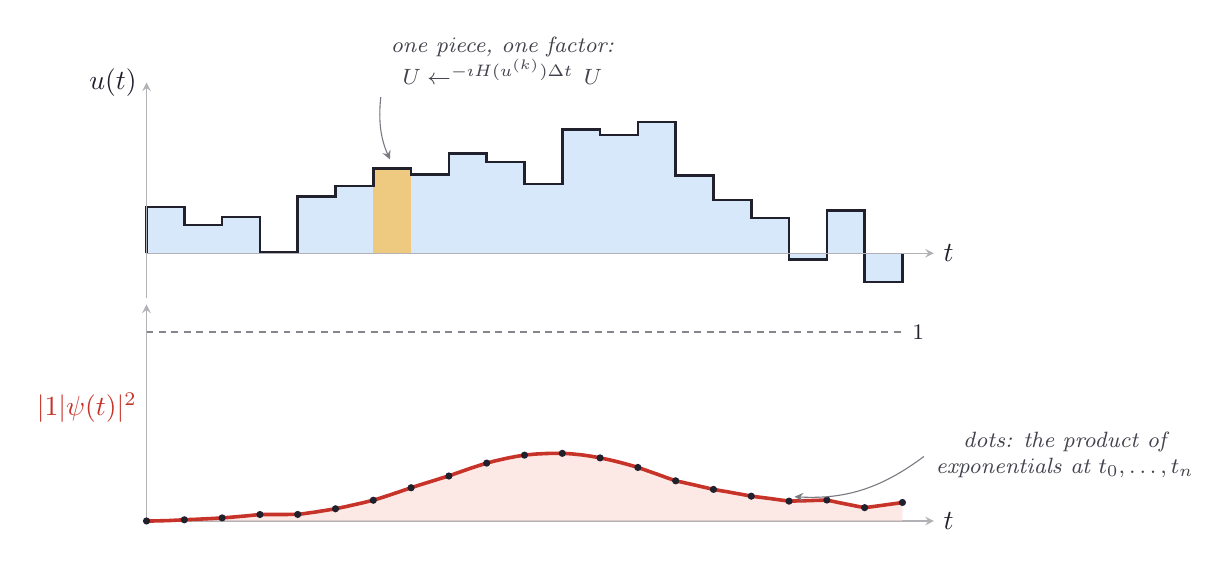
\begin{tikzpicture}[ink/.style={line width=0.9pt, ndInk}, faint/.style={line width=0.4pt, ndInk!35}, dashedink/.style={line width=0.5pt, ndInk!55, dash pattern=on 2.5pt off 2pt}, vec/.style={->, >=stealth, line width=1.2pt}, note/.style={font=\footnotesize\itshape, text=ndInk!85, align=center}, pointer/.style={->, >=stealth, line width=0.4pt, ndInk!60, shorten >=2pt, shorten <=1pt}, dot/.style={circle, fill=ndInk, inner sep=0pt, minimum size=3.4pt}, wash/.style={fill=ndSky, fill opacity=0.55}, every node/.style={text=ndInk}]
\definecolor{ndInk}{rgb}{0.13,0.13,0.18}
\definecolor{ndPaper}{rgb}{0.99,0.96,0.88}
\definecolor{ndSky}{rgb}{0.84,0.91,0.98}
\definecolor{ndRose}{rgb}{0.98,0.86,0.84}
\definecolor{ndBlue}{rgb}{0.13,0.36,0.66}
\definecolor{ndRed}{rgb}{0.78,0.20,0.16}
\definecolor{ndGold}{rgb}{0.88,0.62,0.10}
\definecolor{ndGreen}{rgb}{0.18,0.52,0.30}
\fill[ndSky] (0.000,0) rectangle (0.480,0.590);
\fill[ndSky] (0.480,0) rectangle (0.960,0.361);
\fill[ndSky] (0.960,0) rectangle (1.440,0.460);
\fill[ndSky] (1.440,0) rectangle (1.920,0.013);
\fill[ndSky] (1.920,0) rectangle (2.400,0.719);
\fill[ndSky] (2.400,0) rectangle (2.880,0.854);
\fill[ndGold!55] (2.880,0) rectangle (3.360,1.078);
\fill[ndSky] (3.360,0) rectangle (3.840,1.002);
\fill[ndSky] (3.840,0) rectangle (4.320,1.265);
\fill[ndSky] (4.320,0) rectangle (4.800,1.158);
\fill[ndSky] (4.800,0) rectangle (5.280,0.882);
\fill[ndSky] (5.280,0) rectangle (5.760,1.572);
\fill[ndSky] (5.760,0) rectangle (6.240,1.500);
\fill[ndSky] (6.240,0) rectangle (6.720,1.669);
\fill[ndSky] (6.720,0) rectangle (7.200,0.988);
\fill[ndSky] (7.200,0) rectangle (7.680,0.677);
\fill[ndSky] (7.680,0) rectangle (8.160,0.448);
\fill[ndSky] (8.160,0) rectangle (8.640,-0.082);
\fill[ndSky] (8.640,0) rectangle (9.120,0.541);
\fill[ndSky] (9.120,0) rectangle (9.600,-0.363);
\draw[ink] (0.000,0.000) -- (0.000,0.590) -- (0.480,0.590) -- (0.480,0.361) -- (0.960,0.361) -- (0.960,0.460) -- (1.440,0.460) -- (1.440,0.013) -- (1.920,0.013) -- (1.920,0.719) -- (2.400,0.719) -- (2.400,0.854) -- (2.880,0.854) -- (2.880,1.078) -- (3.360,1.078) -- (3.360,1.002) -- (3.840,1.002) -- (3.840,1.265) -- (4.320,1.265) -- (4.320,1.158) -- (4.800,1.158) -- (4.800,0.882) -- (5.280,0.882) -- (5.280,1.572) -- (5.760,1.572) -- (5.760,1.500) -- (6.240,1.500) -- (6.240,1.669) -- (6.720,1.669) -- (6.720,0.988) -- (7.200,0.988) -- (7.200,0.677) -- (7.680,0.677) -- (7.680,0.448) -- (8.160,0.448) -- (8.160,-0.082) -- (8.640,-0.082) -- (8.640,0.541) -- (9.120,0.541) -- (9.120,-0.363) -- (9.600,-0.363) -- (9.600,0.000);
\draw[faint, ->, >=stealth] (0,0) -- (10.000,0) node[right] {$t$};
\draw[faint, ->, >=stealth] (0,-0.563) -- (0,2.169) node[left] {$u(t)$};
\node[note, anchor=south] (p) at (4.520,2.019) {one piece, one factor:\\$U\leftarrow\ee^{-\imath H(u^{(k)})\Delta t}\,U$};
\draw[pointer] (p.south west) to[bend right=15] (3.120,1.128);
\draw[faint, ->, >=stealth] (0,-3.400) -- (10.000,-3.400) node[right] {$t$};
\draw[faint, ->, >=stealth] (0,-3.400) -- (0,-0.650);
\draw[dashedink] (0,-1.000) -- (9.600,-1.000) node[right, font=\footnotesize] {$1$};
\fill[ndRose, fill opacity=0.6] (0,-3.400) -- (0.000,-3.400) -- (0.040,-3.400) -- (0.080,-3.400) -- (0.120,-3.399) -- (0.160,-3.398) -- (0.200,-3.397) -- (0.240,-3.396) -- (0.280,-3.395) -- (0.320,-3.393) -- (0.360,-3.391) -- (0.400,-3.389) -- (0.440,-3.387) -- (0.480,-3.385) -- (0.520,-3.383) -- (0.560,-3.381) -- (0.600,-3.380) -- (0.640,-3.378) -- (0.680,-3.376) -- (0.720,-3.374) -- (0.760,-3.372) -- (0.800,-3.370) -- (0.840,-3.368) -- (0.880,-3.366) -- (0.920,-3.363) -- (0.960,-3.361) -- (1.000,-3.358) -- (1.040,-3.355) -- (1.080,-3.352) -- (1.120,-3.348) -- (1.160,-3.345) -- (1.200,-3.341) -- (1.240,-3.338) -- (1.280,-3.334) -- (1.320,-3.330) -- (1.360,-3.326) -- (1.400,-3.322) -- (1.440,-3.318) -- (1.480,-3.318) -- (1.520,-3.318) -- (1.560,-3.318) -- (1.600,-3.318) -- (1.640,-3.318) -- (1.680,-3.318) -- (1.720,-3.318) -- (1.760,-3.318) -- (1.800,-3.317) -- (1.840,-3.317) -- (1.880,-3.317) -- (1.920,-3.317) -- (1.960,-3.312) -- (2.000,-3.307) -- (2.040,-3.301) -- (2.080,-3.295) -- (2.120,-3.290) -- (2.160,-3.284) -- (2.200,-3.277) -- (2.240,-3.271) -- (2.280,-3.265) -- (2.320,-3.258) -- (2.360,-3.252) -- (2.400,-3.245) -- (2.440,-3.237) -- (2.480,-3.228) -- (2.520,-3.220) -- (2.560,-3.211) -- (2.600,-3.202) -- (2.640,-3.193) -- (2.680,-3.184) -- (2.720,-3.175) -- (2.760,-3.166) -- (2.800,-3.156) -- (2.840,-3.146) -- (2.880,-3.137) -- (2.920,-3.124) -- (2.960,-3.112) -- (3.000,-3.099) -- (3.040,-3.086) -- (3.080,-3.073) -- (3.120,-3.060) -- (3.160,-3.046) -- (3.200,-3.033) -- (3.240,-3.019) -- (3.280,-3.005) -- (3.320,-2.992) -- (3.360,-2.978) -- (3.400,-2.965) -- (3.440,-2.952) -- (3.480,-2.939) -- (3.520,-2.927) -- (3.560,-2.914) -- (3.600,-2.902) -- (3.640,-2.889) -- (3.680,-2.877) -- (3.720,-2.864) -- (3.760,-2.852) -- (3.800,-2.840) -- (3.840,-2.829) -- (3.880,-2.814) -- (3.920,-2.799) -- (3.960,-2.785) -- (4.000,-2.771) -- (4.040,-2.757) -- (4.080,-2.743) -- (4.120,-2.729) -- (4.160,-2.716) -- (4.200,-2.703) -- (4.240,-2.690) -- (4.280,-2.678) -- (4.320,-2.665) -- (4.360,-2.655) -- (4.400,-2.644) -- (4.440,-2.634) -- (4.480,-2.625) -- (4.520,-2.616) -- (4.560,-2.607) -- (4.600,-2.598) -- (4.640,-2.591) -- (4.680,-2.583) -- (4.720,-2.576) -- (4.760,-2.570) -- (4.800,-2.564) -- (4.840,-2.559) -- (4.880,-2.556) -- (4.920,-2.552) -- (4.960,-2.549) -- (5.000,-2.547) -- (5.040,-2.545) -- (5.080,-2.543) -- (5.120,-2.542) -- (5.160,-2.541) -- (5.200,-2.541) -- (5.240,-2.541) -- (5.280,-2.541) -- (5.320,-2.543) -- (5.360,-2.545) -- (5.400,-2.548) -- (5.440,-2.552) -- (5.480,-2.556) -- (5.520,-2.560) -- (5.560,-2.565) -- (5.600,-2.571) -- (5.640,-2.577) -- (5.680,-2.584) -- (5.720,-2.591) -- (5.760,-2.599) -- (5.800,-2.607) -- (5.840,-2.615) -- (5.880,-2.624) -- (5.920,-2.633) -- (5.960,-2.643) -- (6.000,-2.653) -- (6.040,-2.663) -- (6.080,-2.674) -- (6.120,-2.685) -- (6.160,-2.696) -- (6.200,-2.708) -- (6.240,-2.720) -- (6.280,-2.734) -- (6.320,-2.748) -- (6.360,-2.762) -- (6.400,-2.776) -- (6.440,-2.790) -- (6.480,-2.804) -- (6.520,-2.819) -- (6.560,-2.833) -- (6.600,-2.848) -- (6.640,-2.862) -- (6.680,-2.876) -- (6.720,-2.890) -- (6.760,-2.899) -- (6.800,-2.907) -- (6.840,-2.916) -- (6.880,-2.925) -- (6.920,-2.934) -- (6.960,-2.943) -- (7.000,-2.952) -- (7.040,-2.962) -- (7.080,-2.971) -- (7.120,-2.980) -- (7.160,-2.990) -- (7.200,-2.999) -- (7.240,-3.006) -- (7.280,-3.013) -- (7.320,-3.020) -- (7.360,-3.026) -- (7.400,-3.033) -- (7.440,-3.041) -- (7.480,-3.048) -- (7.520,-3.055) -- (7.560,-3.062) -- (7.600,-3.070) -- (7.640,-3.077) -- (7.680,-3.085) -- (7.720,-3.090) -- (7.760,-3.095) -- (7.800,-3.100) -- (7.840,-3.105) -- (7.880,-3.110) -- (7.920,-3.115) -- (7.960,-3.121) -- (8.000,-3.126) -- (8.040,-3.132) -- (8.080,-3.137) -- (8.120,-3.143) -- (8.160,-3.148) -- (8.200,-3.147) -- (8.240,-3.146) -- (8.280,-3.145) -- (8.320,-3.144) -- (8.360,-3.143) -- (8.400,-3.142) -- (8.440,-3.141) -- (8.480,-3.139) -- (8.520,-3.138) -- (8.560,-3.137) -- (8.600,-3.136) -- (8.640,-3.134) -- (8.680,-3.143) -- (8.720,-3.151) -- (8.760,-3.160) -- (8.800,-3.168) -- (8.840,-3.176) -- (8.880,-3.184) -- (8.920,-3.192) -- (8.960,-3.200) -- (9.000,-3.208) -- (9.040,-3.216) -- (9.080,-3.223) -- (9.120,-3.231) -- (9.164,-3.225) -- (9.207,-3.220) -- (9.251,-3.214) -- (9.295,-3.208) -- (9.338,-3.202) -- (9.382,-3.196) -- (9.425,-3.190) -- (9.469,-3.184) -- (9.513,-3.178) -- (9.556,-3.172) -- (9.600,-3.165) -- (9.600,-3.400) -- cycle;
\draw[line width=1.3pt, ndRed] (0.000,-3.400) -- (0.040,-3.400) -- (0.080,-3.400) -- (0.120,-3.399) -- (0.160,-3.398) -- (0.200,-3.397) -- (0.240,-3.396) -- (0.280,-3.395) -- (0.320,-3.393) -- (0.360,-3.391) -- (0.400,-3.389) -- (0.440,-3.387) -- (0.480,-3.385) -- (0.520,-3.383) -- (0.560,-3.381) -- (0.600,-3.380) -- (0.640,-3.378) -- (0.680,-3.376) -- (0.720,-3.374) -- (0.760,-3.372) -- (0.800,-3.370) -- (0.840,-3.368) -- (0.880,-3.366) -- (0.920,-3.363) -- (0.960,-3.361) -- (1.000,-3.358) -- (1.040,-3.355) -- (1.080,-3.352) -- (1.120,-3.348) -- (1.160,-3.345) -- (1.200,-3.341) -- (1.240,-3.338) -- (1.280,-3.334) -- (1.320,-3.330) -- (1.360,-3.326) -- (1.400,-3.322) -- (1.440,-3.318) -- (1.480,-3.318) -- (1.520,-3.318) -- (1.560,-3.318) -- (1.600,-3.318) -- (1.640,-3.318) -- (1.680,-3.318) -- (1.720,-3.318) -- (1.760,-3.318) -- (1.800,-3.317) -- (1.840,-3.317) -- (1.880,-3.317) -- (1.920,-3.317) -- (1.960,-3.312) -- (2.000,-3.307) -- (2.040,-3.301) -- (2.080,-3.295) -- (2.120,-3.290) -- (2.160,-3.284) -- (2.200,-3.277) -- (2.240,-3.271) -- (2.280,-3.265) -- (2.320,-3.258) -- (2.360,-3.252) -- (2.400,-3.245) -- (2.440,-3.237) -- (2.480,-3.228) -- (2.520,-3.220) -- (2.560,-3.211) -- (2.600,-3.202) -- (2.640,-3.193) -- (2.680,-3.184) -- (2.720,-3.175) -- (2.760,-3.166) -- (2.800,-3.156) -- (2.840,-3.146) -- (2.880,-3.137) -- (2.920,-3.124) -- (2.960,-3.112) -- (3.000,-3.099) -- (3.040,-3.086) -- (3.080,-3.073) -- (3.120,-3.060) -- (3.160,-3.046) -- (3.200,-3.033) -- (3.240,-3.019) -- (3.280,-3.005) -- (3.320,-2.992) -- (3.360,-2.978) -- (3.400,-2.965) -- (3.440,-2.952) -- (3.480,-2.939) -- (3.520,-2.927) -- (3.560,-2.914) -- (3.600,-2.902) -- (3.640,-2.889) -- (3.680,-2.877) -- (3.720,-2.864) -- (3.760,-2.852) -- (3.800,-2.840) -- (3.840,-2.829) -- (3.880,-2.814) -- (3.920,-2.799) -- (3.960,-2.785) -- (4.000,-2.771) -- (4.040,-2.757) -- (4.080,-2.743) -- (4.120,-2.729) -- (4.160,-2.716) -- (4.200,-2.703) -- (4.240,-2.690) -- (4.280,-2.678) -- (4.320,-2.665) -- (4.360,-2.655) -- (4.400,-2.644) -- (4.440,-2.634) -- (4.480,-2.625) -- (4.520,-2.616) -- (4.560,-2.607) -- (4.600,-2.598) -- (4.640,-2.591) -- (4.680,-2.583) -- (4.720,-2.576) -- (4.760,-2.570) -- (4.800,-2.564) -- (4.840,-2.559) -- (4.880,-2.556) -- (4.920,-2.552) -- (4.960,-2.549) -- (5.000,-2.547) -- (5.040,-2.545) -- (5.080,-2.543) -- (5.120,-2.542) -- (5.160,-2.541) -- (5.200,-2.541) -- (5.240,-2.541) -- (5.280,-2.541) -- (5.320,-2.543) -- (5.360,-2.545) -- (5.400,-2.548) -- (5.440,-2.552) -- (5.480,-2.556) -- (5.520,-2.560) -- (5.560,-2.565) -- (5.600,-2.571) -- (5.640,-2.577) -- (5.680,-2.584) -- (5.720,-2.591) -- (5.760,-2.599) -- (5.800,-2.607) -- (5.840,-2.615) -- (5.880,-2.624) -- (5.920,-2.633) -- (5.960,-2.643) -- (6.000,-2.653) -- (6.040,-2.663) -- (6.080,-2.674) -- (6.120,-2.685) -- (6.160,-2.696) -- (6.200,-2.708) -- (6.240,-2.720) -- (6.280,-2.734) -- (6.320,-2.748) -- (6.360,-2.762) -- (6.400,-2.776) -- (6.440,-2.790) -- (6.480,-2.804) -- (6.520,-2.819) -- (6.560,-2.833) -- (6.600,-2.848) -- (6.640,-2.862) -- (6.680,-2.876) -- (6.720,-2.890) -- (6.760,-2.899) -- (6.800,-2.907) -- (6.840,-2.916) -- (6.880,-2.925) -- (6.920,-2.934) -- (6.960,-2.943) -- (7.000,-2.952) -- (7.040,-2.962) -- (7.080,-2.971) -- (7.120,-2.980) -- (7.160,-2.990) -- (7.200,-2.999) -- (7.240,-3.006) -- (7.280,-3.013) -- (7.320,-3.020) -- (7.360,-3.026) -- (7.400,-3.033) -- (7.440,-3.041) -- (7.480,-3.048) -- (7.520,-3.055) -- (7.560,-3.062) -- (7.600,-3.070) -- (7.640,-3.077) -- (7.680,-3.085) -- (7.720,-3.090) -- (7.760,-3.095) -- (7.800,-3.100) -- (7.840,-3.105) -- (7.880,-3.110) -- (7.920,-3.115) -- (7.960,-3.121) -- (8.000,-3.126) -- (8.040,-3.132) -- (8.080,-3.137) -- (8.120,-3.143) -- (8.160,-3.148) -- (8.200,-3.147) -- (8.240,-3.146) -- (8.280,-3.145) -- (8.320,-3.144) -- (8.360,-3.143) -- (8.400,-3.142) -- (8.440,-3.141) -- (8.480,-3.139) -- (8.520,-3.138) -- (8.560,-3.137) -- (8.600,-3.136) -- (8.640,-3.134) -- (8.680,-3.143) -- (8.720,-3.151) -- (8.760,-3.160) -- (8.800,-3.168) -- (8.840,-3.176) -- (8.880,-3.184) -- (8.920,-3.192) -- (8.960,-3.200) -- (9.000,-3.208) -- (9.040,-3.216) -- (9.080,-3.223) -- (9.120,-3.231) -- (9.164,-3.225) -- (9.207,-3.220) -- (9.251,-3.214) -- (9.295,-3.208) -- (9.338,-3.202) -- (9.382,-3.196) -- (9.425,-3.190) -- (9.469,-3.184) -- (9.513,-3.178) -- (9.556,-3.172) -- (9.600,-3.165);
\fill[ndInk] (0.000,-3.400) circle (1.3pt);
\fill[ndInk] (0.480,-3.385) circle (1.3pt);
\fill[ndInk] (0.960,-3.361) circle (1.3pt);
\fill[ndInk] (1.440,-3.318) circle (1.3pt);
\fill[ndInk] (1.920,-3.317) circle (1.3pt);
\fill[ndInk] (2.400,-3.245) circle (1.3pt);
\fill[ndInk] (2.880,-3.137) circle (1.3pt);
\fill[ndInk] (3.360,-2.978) circle (1.3pt);
\fill[ndInk] (3.840,-2.829) circle (1.3pt);
\fill[ndInk] (4.320,-2.665) circle (1.3pt);
\fill[ndInk] (4.800,-2.564) circle (1.3pt);
\fill[ndInk] (5.280,-2.541) circle (1.3pt);
\fill[ndInk] (5.760,-2.599) circle (1.3pt);
\fill[ndInk] (6.240,-2.720) circle (1.3pt);
\fill[ndInk] (6.720,-2.890) circle (1.3pt);
\fill[ndInk] (7.200,-2.999) circle (1.3pt);
\fill[ndInk] (7.680,-3.085) circle (1.3pt);
\fill[ndInk] (8.160,-3.148) circle (1.3pt);
\fill[ndInk] (8.640,-3.134) circle (1.3pt);
\fill[ndInk] (9.120,-3.231) circle (1.3pt);
\fill[ndInk] (9.600,-3.165) circle (1.3pt);
\node[left, text=ndRed] at (0,-1.960) {$|\braket{1|\psi(t)}|^2$};
\node[note, anchor=west] (d) at (9.900,-2.560) {dots: the product of\\ exponentials at $t_0,\dots,t_n$};
\draw[pointer] (d.west) to[bend left=20] (8.160,-3.088);
\end{tikzpicture}

\caption{A piecewise-constant control (step function) and the population $\abs{\braket{1|\psi(t)}}^2$ it produces on a qubit with drift $\tfrac12\sigma_z$ and control Hamiltonian $\tfrac12\sigma_x$. Generated by \texttt{code/ch02\_pwc.py}.}\label{fig:ch02:pwc}
\end{figure}}
\onp{\begin{center}\resizebox{!}{0.56\textheight}{% Generated by code/needham.py -- do not edit by hand.
\definecolor{qocA}{rgb}{0.00,0.45,0.70}
\definecolor{qocB}{rgb}{0.90,0.60,0.00}
\definecolor{qocC}{rgb}{0.00,0.62,0.45}
\definecolor{qocD}{rgb}{0.80,0.40,0.00}
\definecolor{qocE}{rgb}{0.80,0.60,0.70}
\definecolor{qocF}{rgb}{0.35,0.70,0.90}
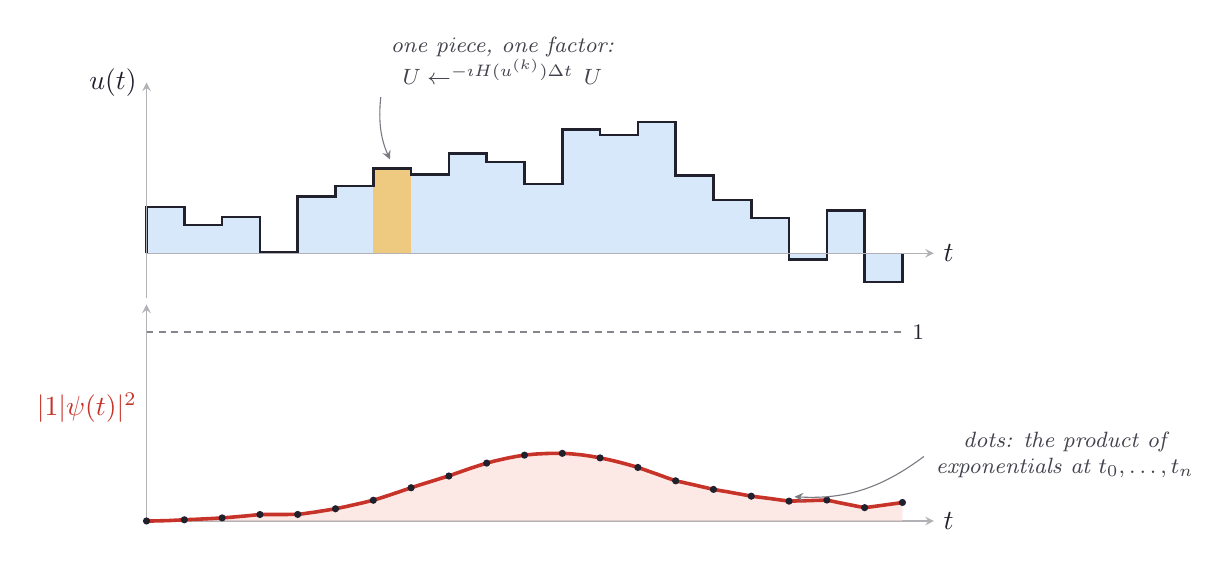
\begin{tikzpicture}[ink/.style={line width=0.9pt, ndInk}, faint/.style={line width=0.4pt, ndInk!35}, dashedink/.style={line width=0.5pt, ndInk!55, dash pattern=on 2.5pt off 2pt}, vec/.style={->, >=stealth, line width=1.2pt}, note/.style={font=\footnotesize\itshape, text=ndInk!85, align=center}, pointer/.style={->, >=stealth, line width=0.4pt, ndInk!60, shorten >=2pt, shorten <=1pt}, dot/.style={circle, fill=ndInk, inner sep=0pt, minimum size=3.4pt}, wash/.style={fill=ndSky, fill opacity=0.55}, every node/.style={text=ndInk}]
\definecolor{ndInk}{rgb}{0.13,0.13,0.18}
\definecolor{ndPaper}{rgb}{0.99,0.96,0.88}
\definecolor{ndSky}{rgb}{0.84,0.91,0.98}
\definecolor{ndRose}{rgb}{0.98,0.86,0.84}
\definecolor{ndBlue}{rgb}{0.13,0.36,0.66}
\definecolor{ndRed}{rgb}{0.78,0.20,0.16}
\definecolor{ndGold}{rgb}{0.88,0.62,0.10}
\definecolor{ndGreen}{rgb}{0.18,0.52,0.30}
\fill[ndSky] (0.000,0) rectangle (0.480,0.590);
\fill[ndSky] (0.480,0) rectangle (0.960,0.361);
\fill[ndSky] (0.960,0) rectangle (1.440,0.460);
\fill[ndSky] (1.440,0) rectangle (1.920,0.013);
\fill[ndSky] (1.920,0) rectangle (2.400,0.719);
\fill[ndSky] (2.400,0) rectangle (2.880,0.854);
\fill[ndGold!55] (2.880,0) rectangle (3.360,1.078);
\fill[ndSky] (3.360,0) rectangle (3.840,1.002);
\fill[ndSky] (3.840,0) rectangle (4.320,1.265);
\fill[ndSky] (4.320,0) rectangle (4.800,1.158);
\fill[ndSky] (4.800,0) rectangle (5.280,0.882);
\fill[ndSky] (5.280,0) rectangle (5.760,1.572);
\fill[ndSky] (5.760,0) rectangle (6.240,1.500);
\fill[ndSky] (6.240,0) rectangle (6.720,1.669);
\fill[ndSky] (6.720,0) rectangle (7.200,0.988);
\fill[ndSky] (7.200,0) rectangle (7.680,0.677);
\fill[ndSky] (7.680,0) rectangle (8.160,0.448);
\fill[ndSky] (8.160,0) rectangle (8.640,-0.082);
\fill[ndSky] (8.640,0) rectangle (9.120,0.541);
\fill[ndSky] (9.120,0) rectangle (9.600,-0.363);
\draw[ink] (0.000,0.000) -- (0.000,0.590) -- (0.480,0.590) -- (0.480,0.361) -- (0.960,0.361) -- (0.960,0.460) -- (1.440,0.460) -- (1.440,0.013) -- (1.920,0.013) -- (1.920,0.719) -- (2.400,0.719) -- (2.400,0.854) -- (2.880,0.854) -- (2.880,1.078) -- (3.360,1.078) -- (3.360,1.002) -- (3.840,1.002) -- (3.840,1.265) -- (4.320,1.265) -- (4.320,1.158) -- (4.800,1.158) -- (4.800,0.882) -- (5.280,0.882) -- (5.280,1.572) -- (5.760,1.572) -- (5.760,1.500) -- (6.240,1.500) -- (6.240,1.669) -- (6.720,1.669) -- (6.720,0.988) -- (7.200,0.988) -- (7.200,0.677) -- (7.680,0.677) -- (7.680,0.448) -- (8.160,0.448) -- (8.160,-0.082) -- (8.640,-0.082) -- (8.640,0.541) -- (9.120,0.541) -- (9.120,-0.363) -- (9.600,-0.363) -- (9.600,0.000);
\draw[faint, ->, >=stealth] (0,0) -- (10.000,0) node[right] {$t$};
\draw[faint, ->, >=stealth] (0,-0.563) -- (0,2.169) node[left] {$u(t)$};
\node[note, anchor=south] (p) at (4.520,2.019) {one piece, one factor:\\$U\leftarrow\ee^{-\imath H(u^{(k)})\Delta t}\,U$};
\draw[pointer] (p.south west) to[bend right=15] (3.120,1.128);
\draw[faint, ->, >=stealth] (0,-3.400) -- (10.000,-3.400) node[right] {$t$};
\draw[faint, ->, >=stealth] (0,-3.400) -- (0,-0.650);
\draw[dashedink] (0,-1.000) -- (9.600,-1.000) node[right, font=\footnotesize] {$1$};
\fill[ndRose, fill opacity=0.6] (0,-3.400) -- (0.000,-3.400) -- (0.040,-3.400) -- (0.080,-3.400) -- (0.120,-3.399) -- (0.160,-3.398) -- (0.200,-3.397) -- (0.240,-3.396) -- (0.280,-3.395) -- (0.320,-3.393) -- (0.360,-3.391) -- (0.400,-3.389) -- (0.440,-3.387) -- (0.480,-3.385) -- (0.520,-3.383) -- (0.560,-3.381) -- (0.600,-3.380) -- (0.640,-3.378) -- (0.680,-3.376) -- (0.720,-3.374) -- (0.760,-3.372) -- (0.800,-3.370) -- (0.840,-3.368) -- (0.880,-3.366) -- (0.920,-3.363) -- (0.960,-3.361) -- (1.000,-3.358) -- (1.040,-3.355) -- (1.080,-3.352) -- (1.120,-3.348) -- (1.160,-3.345) -- (1.200,-3.341) -- (1.240,-3.338) -- (1.280,-3.334) -- (1.320,-3.330) -- (1.360,-3.326) -- (1.400,-3.322) -- (1.440,-3.318) -- (1.480,-3.318) -- (1.520,-3.318) -- (1.560,-3.318) -- (1.600,-3.318) -- (1.640,-3.318) -- (1.680,-3.318) -- (1.720,-3.318) -- (1.760,-3.318) -- (1.800,-3.317) -- (1.840,-3.317) -- (1.880,-3.317) -- (1.920,-3.317) -- (1.960,-3.312) -- (2.000,-3.307) -- (2.040,-3.301) -- (2.080,-3.295) -- (2.120,-3.290) -- (2.160,-3.284) -- (2.200,-3.277) -- (2.240,-3.271) -- (2.280,-3.265) -- (2.320,-3.258) -- (2.360,-3.252) -- (2.400,-3.245) -- (2.440,-3.237) -- (2.480,-3.228) -- (2.520,-3.220) -- (2.560,-3.211) -- (2.600,-3.202) -- (2.640,-3.193) -- (2.680,-3.184) -- (2.720,-3.175) -- (2.760,-3.166) -- (2.800,-3.156) -- (2.840,-3.146) -- (2.880,-3.137) -- (2.920,-3.124) -- (2.960,-3.112) -- (3.000,-3.099) -- (3.040,-3.086) -- (3.080,-3.073) -- (3.120,-3.060) -- (3.160,-3.046) -- (3.200,-3.033) -- (3.240,-3.019) -- (3.280,-3.005) -- (3.320,-2.992) -- (3.360,-2.978) -- (3.400,-2.965) -- (3.440,-2.952) -- (3.480,-2.939) -- (3.520,-2.927) -- (3.560,-2.914) -- (3.600,-2.902) -- (3.640,-2.889) -- (3.680,-2.877) -- (3.720,-2.864) -- (3.760,-2.852) -- (3.800,-2.840) -- (3.840,-2.829) -- (3.880,-2.814) -- (3.920,-2.799) -- (3.960,-2.785) -- (4.000,-2.771) -- (4.040,-2.757) -- (4.080,-2.743) -- (4.120,-2.729) -- (4.160,-2.716) -- (4.200,-2.703) -- (4.240,-2.690) -- (4.280,-2.678) -- (4.320,-2.665) -- (4.360,-2.655) -- (4.400,-2.644) -- (4.440,-2.634) -- (4.480,-2.625) -- (4.520,-2.616) -- (4.560,-2.607) -- (4.600,-2.598) -- (4.640,-2.591) -- (4.680,-2.583) -- (4.720,-2.576) -- (4.760,-2.570) -- (4.800,-2.564) -- (4.840,-2.559) -- (4.880,-2.556) -- (4.920,-2.552) -- (4.960,-2.549) -- (5.000,-2.547) -- (5.040,-2.545) -- (5.080,-2.543) -- (5.120,-2.542) -- (5.160,-2.541) -- (5.200,-2.541) -- (5.240,-2.541) -- (5.280,-2.541) -- (5.320,-2.543) -- (5.360,-2.545) -- (5.400,-2.548) -- (5.440,-2.552) -- (5.480,-2.556) -- (5.520,-2.560) -- (5.560,-2.565) -- (5.600,-2.571) -- (5.640,-2.577) -- (5.680,-2.584) -- (5.720,-2.591) -- (5.760,-2.599) -- (5.800,-2.607) -- (5.840,-2.615) -- (5.880,-2.624) -- (5.920,-2.633) -- (5.960,-2.643) -- (6.000,-2.653) -- (6.040,-2.663) -- (6.080,-2.674) -- (6.120,-2.685) -- (6.160,-2.696) -- (6.200,-2.708) -- (6.240,-2.720) -- (6.280,-2.734) -- (6.320,-2.748) -- (6.360,-2.762) -- (6.400,-2.776) -- (6.440,-2.790) -- (6.480,-2.804) -- (6.520,-2.819) -- (6.560,-2.833) -- (6.600,-2.848) -- (6.640,-2.862) -- (6.680,-2.876) -- (6.720,-2.890) -- (6.760,-2.899) -- (6.800,-2.907) -- (6.840,-2.916) -- (6.880,-2.925) -- (6.920,-2.934) -- (6.960,-2.943) -- (7.000,-2.952) -- (7.040,-2.962) -- (7.080,-2.971) -- (7.120,-2.980) -- (7.160,-2.990) -- (7.200,-2.999) -- (7.240,-3.006) -- (7.280,-3.013) -- (7.320,-3.020) -- (7.360,-3.026) -- (7.400,-3.033) -- (7.440,-3.041) -- (7.480,-3.048) -- (7.520,-3.055) -- (7.560,-3.062) -- (7.600,-3.070) -- (7.640,-3.077) -- (7.680,-3.085) -- (7.720,-3.090) -- (7.760,-3.095) -- (7.800,-3.100) -- (7.840,-3.105) -- (7.880,-3.110) -- (7.920,-3.115) -- (7.960,-3.121) -- (8.000,-3.126) -- (8.040,-3.132) -- (8.080,-3.137) -- (8.120,-3.143) -- (8.160,-3.148) -- (8.200,-3.147) -- (8.240,-3.146) -- (8.280,-3.145) -- (8.320,-3.144) -- (8.360,-3.143) -- (8.400,-3.142) -- (8.440,-3.141) -- (8.480,-3.139) -- (8.520,-3.138) -- (8.560,-3.137) -- (8.600,-3.136) -- (8.640,-3.134) -- (8.680,-3.143) -- (8.720,-3.151) -- (8.760,-3.160) -- (8.800,-3.168) -- (8.840,-3.176) -- (8.880,-3.184) -- (8.920,-3.192) -- (8.960,-3.200) -- (9.000,-3.208) -- (9.040,-3.216) -- (9.080,-3.223) -- (9.120,-3.231) -- (9.164,-3.225) -- (9.207,-3.220) -- (9.251,-3.214) -- (9.295,-3.208) -- (9.338,-3.202) -- (9.382,-3.196) -- (9.425,-3.190) -- (9.469,-3.184) -- (9.513,-3.178) -- (9.556,-3.172) -- (9.600,-3.165) -- (9.600,-3.400) -- cycle;
\draw[line width=1.3pt, ndRed] (0.000,-3.400) -- (0.040,-3.400) -- (0.080,-3.400) -- (0.120,-3.399) -- (0.160,-3.398) -- (0.200,-3.397) -- (0.240,-3.396) -- (0.280,-3.395) -- (0.320,-3.393) -- (0.360,-3.391) -- (0.400,-3.389) -- (0.440,-3.387) -- (0.480,-3.385) -- (0.520,-3.383) -- (0.560,-3.381) -- (0.600,-3.380) -- (0.640,-3.378) -- (0.680,-3.376) -- (0.720,-3.374) -- (0.760,-3.372) -- (0.800,-3.370) -- (0.840,-3.368) -- (0.880,-3.366) -- (0.920,-3.363) -- (0.960,-3.361) -- (1.000,-3.358) -- (1.040,-3.355) -- (1.080,-3.352) -- (1.120,-3.348) -- (1.160,-3.345) -- (1.200,-3.341) -- (1.240,-3.338) -- (1.280,-3.334) -- (1.320,-3.330) -- (1.360,-3.326) -- (1.400,-3.322) -- (1.440,-3.318) -- (1.480,-3.318) -- (1.520,-3.318) -- (1.560,-3.318) -- (1.600,-3.318) -- (1.640,-3.318) -- (1.680,-3.318) -- (1.720,-3.318) -- (1.760,-3.318) -- (1.800,-3.317) -- (1.840,-3.317) -- (1.880,-3.317) -- (1.920,-3.317) -- (1.960,-3.312) -- (2.000,-3.307) -- (2.040,-3.301) -- (2.080,-3.295) -- (2.120,-3.290) -- (2.160,-3.284) -- (2.200,-3.277) -- (2.240,-3.271) -- (2.280,-3.265) -- (2.320,-3.258) -- (2.360,-3.252) -- (2.400,-3.245) -- (2.440,-3.237) -- (2.480,-3.228) -- (2.520,-3.220) -- (2.560,-3.211) -- (2.600,-3.202) -- (2.640,-3.193) -- (2.680,-3.184) -- (2.720,-3.175) -- (2.760,-3.166) -- (2.800,-3.156) -- (2.840,-3.146) -- (2.880,-3.137) -- (2.920,-3.124) -- (2.960,-3.112) -- (3.000,-3.099) -- (3.040,-3.086) -- (3.080,-3.073) -- (3.120,-3.060) -- (3.160,-3.046) -- (3.200,-3.033) -- (3.240,-3.019) -- (3.280,-3.005) -- (3.320,-2.992) -- (3.360,-2.978) -- (3.400,-2.965) -- (3.440,-2.952) -- (3.480,-2.939) -- (3.520,-2.927) -- (3.560,-2.914) -- (3.600,-2.902) -- (3.640,-2.889) -- (3.680,-2.877) -- (3.720,-2.864) -- (3.760,-2.852) -- (3.800,-2.840) -- (3.840,-2.829) -- (3.880,-2.814) -- (3.920,-2.799) -- (3.960,-2.785) -- (4.000,-2.771) -- (4.040,-2.757) -- (4.080,-2.743) -- (4.120,-2.729) -- (4.160,-2.716) -- (4.200,-2.703) -- (4.240,-2.690) -- (4.280,-2.678) -- (4.320,-2.665) -- (4.360,-2.655) -- (4.400,-2.644) -- (4.440,-2.634) -- (4.480,-2.625) -- (4.520,-2.616) -- (4.560,-2.607) -- (4.600,-2.598) -- (4.640,-2.591) -- (4.680,-2.583) -- (4.720,-2.576) -- (4.760,-2.570) -- (4.800,-2.564) -- (4.840,-2.559) -- (4.880,-2.556) -- (4.920,-2.552) -- (4.960,-2.549) -- (5.000,-2.547) -- (5.040,-2.545) -- (5.080,-2.543) -- (5.120,-2.542) -- (5.160,-2.541) -- (5.200,-2.541) -- (5.240,-2.541) -- (5.280,-2.541) -- (5.320,-2.543) -- (5.360,-2.545) -- (5.400,-2.548) -- (5.440,-2.552) -- (5.480,-2.556) -- (5.520,-2.560) -- (5.560,-2.565) -- (5.600,-2.571) -- (5.640,-2.577) -- (5.680,-2.584) -- (5.720,-2.591) -- (5.760,-2.599) -- (5.800,-2.607) -- (5.840,-2.615) -- (5.880,-2.624) -- (5.920,-2.633) -- (5.960,-2.643) -- (6.000,-2.653) -- (6.040,-2.663) -- (6.080,-2.674) -- (6.120,-2.685) -- (6.160,-2.696) -- (6.200,-2.708) -- (6.240,-2.720) -- (6.280,-2.734) -- (6.320,-2.748) -- (6.360,-2.762) -- (6.400,-2.776) -- (6.440,-2.790) -- (6.480,-2.804) -- (6.520,-2.819) -- (6.560,-2.833) -- (6.600,-2.848) -- (6.640,-2.862) -- (6.680,-2.876) -- (6.720,-2.890) -- (6.760,-2.899) -- (6.800,-2.907) -- (6.840,-2.916) -- (6.880,-2.925) -- (6.920,-2.934) -- (6.960,-2.943) -- (7.000,-2.952) -- (7.040,-2.962) -- (7.080,-2.971) -- (7.120,-2.980) -- (7.160,-2.990) -- (7.200,-2.999) -- (7.240,-3.006) -- (7.280,-3.013) -- (7.320,-3.020) -- (7.360,-3.026) -- (7.400,-3.033) -- (7.440,-3.041) -- (7.480,-3.048) -- (7.520,-3.055) -- (7.560,-3.062) -- (7.600,-3.070) -- (7.640,-3.077) -- (7.680,-3.085) -- (7.720,-3.090) -- (7.760,-3.095) -- (7.800,-3.100) -- (7.840,-3.105) -- (7.880,-3.110) -- (7.920,-3.115) -- (7.960,-3.121) -- (8.000,-3.126) -- (8.040,-3.132) -- (8.080,-3.137) -- (8.120,-3.143) -- (8.160,-3.148) -- (8.200,-3.147) -- (8.240,-3.146) -- (8.280,-3.145) -- (8.320,-3.144) -- (8.360,-3.143) -- (8.400,-3.142) -- (8.440,-3.141) -- (8.480,-3.139) -- (8.520,-3.138) -- (8.560,-3.137) -- (8.600,-3.136) -- (8.640,-3.134) -- (8.680,-3.143) -- (8.720,-3.151) -- (8.760,-3.160) -- (8.800,-3.168) -- (8.840,-3.176) -- (8.880,-3.184) -- (8.920,-3.192) -- (8.960,-3.200) -- (9.000,-3.208) -- (9.040,-3.216) -- (9.080,-3.223) -- (9.120,-3.231) -- (9.164,-3.225) -- (9.207,-3.220) -- (9.251,-3.214) -- (9.295,-3.208) -- (9.338,-3.202) -- (9.382,-3.196) -- (9.425,-3.190) -- (9.469,-3.184) -- (9.513,-3.178) -- (9.556,-3.172) -- (9.600,-3.165);
\fill[ndInk] (0.000,-3.400) circle (1.3pt);
\fill[ndInk] (0.480,-3.385) circle (1.3pt);
\fill[ndInk] (0.960,-3.361) circle (1.3pt);
\fill[ndInk] (1.440,-3.318) circle (1.3pt);
\fill[ndInk] (1.920,-3.317) circle (1.3pt);
\fill[ndInk] (2.400,-3.245) circle (1.3pt);
\fill[ndInk] (2.880,-3.137) circle (1.3pt);
\fill[ndInk] (3.360,-2.978) circle (1.3pt);
\fill[ndInk] (3.840,-2.829) circle (1.3pt);
\fill[ndInk] (4.320,-2.665) circle (1.3pt);
\fill[ndInk] (4.800,-2.564) circle (1.3pt);
\fill[ndInk] (5.280,-2.541) circle (1.3pt);
\fill[ndInk] (5.760,-2.599) circle (1.3pt);
\fill[ndInk] (6.240,-2.720) circle (1.3pt);
\fill[ndInk] (6.720,-2.890) circle (1.3pt);
\fill[ndInk] (7.200,-2.999) circle (1.3pt);
\fill[ndInk] (7.680,-3.085) circle (1.3pt);
\fill[ndInk] (8.160,-3.148) circle (1.3pt);
\fill[ndInk] (8.640,-3.134) circle (1.3pt);
\fill[ndInk] (9.120,-3.231) circle (1.3pt);
\fill[ndInk] (9.600,-3.165) circle (1.3pt);
\node[left, text=ndRed] at (0,-1.960) {$|\braket{1|\psi(t)}|^2$};
\node[note, anchor=west] (d) at (9.900,-2.560) {dots: the product of\\ exponentials at $t_0,\dots,t_n$};
\draw[pointer] (d.west) to[bend left=20] (8.160,-3.088);
\end{tikzpicture}
}\end{center}}
\end{frame}

\section{Reachable sets}\label{sec:ch02:reach}

\begin{frame}\ft{Reachable sets}
\begin{defn}\label{def:reach}
The reachable set at time $T$ from $\Id$ is $\Reach_T=\{U(T): u \text{ admissible}\}$, and $\Reach=\bigcup_{T\ge0}\Reach_T$.
\end{defn}
\begin{thm}[Jurdjevic--Sussmann; preview]\label{thm:js-preview}
Let $\mathfrak L$ be the dynamical Lie algebra of \eqref{eq:bilinear-group}, and let $\ee^{\mathfrak L}\subseteq\Un[N]$ be the connected Lie subgroup with Lie algebra $\mathfrak L$. Let the admissible controls be $u\in L^\infty([0,T];\mathcal U)$, where the affine hull of $\mathcal U$ is $\R^m$ (e.g.\ a box). Then $\Reach\subseteq\ee^{\mathfrak L}$. If $\ee^{\mathfrak L}$ is compact, then $\Reach=\ee^{\mathfrak L}$, and piecewise-constant controls already suffice.
\end{thm}
\begin{cor}\label{cor:ch02:controllable}
Every $U\in\SU[N]$ is reachable, up to a global phase, if and only if $\liesu[N]\subseteq\mathfrak L$.
\end{cor}
\ona{\emph{The hypotheses.} For every Lie subalgebra $\mathfrak L\subseteq\lieu[N]$ there is exactly one connected Lie subgroup $\ee^{\mathfrak L}$ with Lie algebra $\mathfrak L$: the subgroup generated by all $\ee^{X}$, $X\in\mathfrak L$. It may be immersed rather than closed, like the dense line on the torus of Section~\ref{sec:ch02:lie}. Compactness excludes this, since a compact subgroup is closed. It also matters for the dynamics, as explained below: it lets the system wait for the drift to come back instead of reversing it. For the corollary, if $\liesu[N]\subseteq\mathfrak L$ then $\ee^{\mathfrak L}$ is $\SU[N]$ or $\Un[N]$, both compact. Conversely, if every element of $\SU[N]$ is reachable up to phase, the projection of $\mathfrak L$ onto $\liesu[N]$ is onto. Since $\imath\R\Id$ commutes with everything, $\comm{\mathfrak L}{\mathfrak L}=\comm{\liesu[N]}{\liesu[N]}=\liesu[N]$, and $\comm{\mathfrak L}{\mathfrak L}\subseteq\mathfrak L$.}
\end{frame}

\begin{frame}\ft{Reachable sets grow with time}
\ona{Figure~\ref{fig:ch02:reach} makes the reachable sets concrete for a resonant qubit with a bounded drive, $H=\tfrac12(u_x\sigx+u_y\sigy)$ with $u_x^2+u_y^2\le M^2$. The Bloch vector moves with speed $\abs{\vec h\times\Bloch}\le M$. The states reachable from $\ket0$ at time $T$ are therefore those within angular distance $MT$ of the north pole: a spherical cap that grows with $T$. Every point of the cap is reached by a rotation about a horizontal axis, slowed down if necessary. A target at polar angle $\alpha$ enters the reachable set at the moment of first contact, $T_{\min}=\alpha/M$, and the time-optimal path is the meridian. This first-contact picture of the minimum time returns in \Chaps~\ref{C.GeometryControl} and~\ref{C.Complexity}. The figure shows reachable \emph{states}, the images of the reachable unitaries under $U\mapsto U\ket0$; the reachable unitaries themselves behave differently. With $\sigx$ and $\sigy$ controls, a rotation about the $z$-axis cannot be applied directly, and $\ket0$ is blind to it, since it only changes the phase of $\ket0$. As a unitary, however, it has to be produced by loops of $x$- and $y$-rotations as in Figure~\ref{fig:ch02:lie}, at extra cost in time. The reachable sets $\Reach_T\subseteq\SU[2]$ are therefore not ``round'': they are balls of a \emph{sub-Riemannian} geometry, in which only some directions can be followed directly. The caps are their shadows on the sphere of states (\Chap~\ref{C.GeometryControl}).}
\ona{\begin{figure}[h]\centering
\resizebox{0.85\linewidth}{!}{% Generated by code/needham.py -- do not edit by hand.
\definecolor{qocA}{rgb}{0.00,0.45,0.70}
\definecolor{qocB}{rgb}{0.90,0.60,0.00}
\definecolor{qocC}{rgb}{0.00,0.62,0.45}
\definecolor{qocD}{rgb}{0.80,0.40,0.00}
\definecolor{qocE}{rgb}{0.80,0.60,0.70}
\definecolor{qocF}{rgb}{0.35,0.70,0.90}
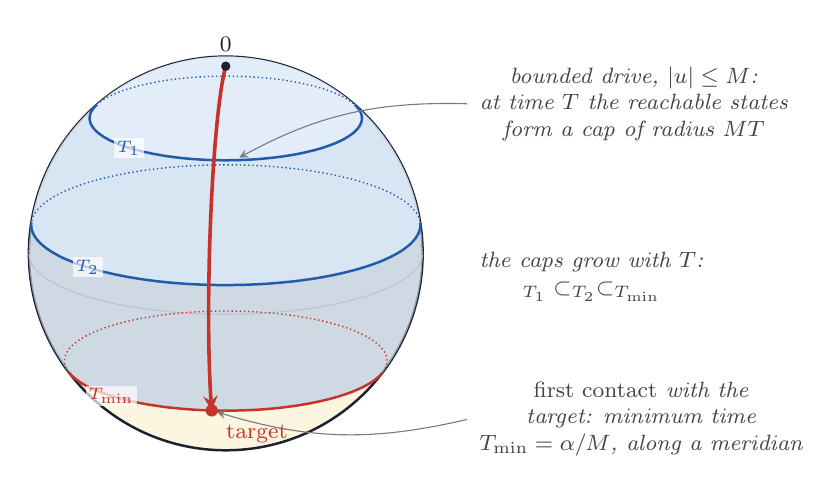
\begin{tikzpicture}[ink/.style={line width=0.9pt, ndInk}, faint/.style={line width=0.4pt, ndInk!35}, dashedink/.style={line width=0.5pt, ndInk!55, dash pattern=on 2.5pt off 2pt}, vec/.style={->, >=stealth, line width=1.2pt}, note/.style={font=\footnotesize\itshape, text=ndInk!85, align=center}, pointer/.style={->, >=stealth, line width=0.4pt, ndInk!60, shorten >=2pt, shorten <=1pt}, dot/.style={circle, fill=ndInk, inner sep=0pt, minimum size=3.4pt}, wash/.style={fill=ndSky, fill opacity=0.55}, every node/.style={text=ndInk}]
\definecolor{ndInk}{rgb}{0.13,0.13,0.18}
\definecolor{ndPaper}{rgb}{0.99,0.96,0.88}
\definecolor{ndSky}{rgb}{0.84,0.91,0.98}
\definecolor{ndRose}{rgb}{0.98,0.86,0.84}
\definecolor{ndBlue}{rgb}{0.13,0.36,0.66}
\definecolor{ndRed}{rgb}{0.78,0.20,0.16}
\definecolor{ndGold}{rgb}{0.88,0.62,0.10}
\definecolor{ndGreen}{rgb}{0.18,0.52,0.30}
\fill[ndPaper] (0.000,0.000) circle (2.500);
\draw[ink] (0.000,0.000) circle (2.500);
\draw[faint] (2.266,-0.326) -- (2.293,-0.308) -- (2.318,-0.289) -- (2.342,-0.271) -- (2.364,-0.252) -- (2.384,-0.232) -- (2.403,-0.213) -- (2.420,-0.193) -- (2.436,-0.174) -- (2.450,-0.154) -- (2.462,-0.134) -- (2.473,-0.114) -- (2.481,-0.094) -- (2.488,-0.074) -- (2.494,-0.054) -- (2.498,-0.034) -- (2.500,-0.013);
\draw[faint] (-2.500,-0.007) -- (-2.498,-0.027) -- (-2.495,-0.047) -- (-2.490,-0.067) -- (-2.484,-0.087) -- (-2.476,-0.108) -- (-2.466,-0.128) -- (-2.454,-0.147) -- (-2.441,-0.167) -- (-2.426,-0.187) -- (-2.409,-0.206) -- (-2.391,-0.226) -- (-2.371,-0.245) -- (-2.349,-0.264) -- (-2.326,-0.283) -- (-2.301,-0.302) -- (-2.275,-0.320) -- (-2.247,-0.339) -- (-2.218,-0.357) -- (-2.187,-0.375) -- (-2.154,-0.392) -- (-2.120,-0.409) -- (-2.085,-0.426) -- (-2.048,-0.443) -- (-2.010,-0.460) -- (-1.970,-0.476) -- (-1.929,-0.491) -- (-1.887,-0.507) -- (-1.843,-0.522) -- (-1.798,-0.537) -- (-1.752,-0.551) -- (-1.705,-0.565) -- (-1.657,-0.579) -- (-1.607,-0.592) -- (-1.556,-0.605) -- (-1.505,-0.617) -- (-1.452,-0.629) -- (-1.398,-0.640) -- (-1.343,-0.652) -- (-1.288,-0.662) -- (-1.231,-0.672) -- (-1.174,-0.682) -- (-1.115,-0.691) -- (-1.057,-0.700) -- (-0.997,-0.708) -- (-0.937,-0.716) -- (-0.876,-0.724) -- (-0.814,-0.730) -- (-0.752,-0.737) -- (-0.689,-0.743) -- (-0.626,-0.748) -- (-0.562,-0.753) -- (-0.498,-0.757) -- (-0.434,-0.761) -- (-0.370,-0.764) -- (-0.305,-0.767) -- (-0.240,-0.769) -- (-0.174,-0.771) -- (-0.109,-0.772) -- (-0.044,-0.772) -- (0.022,-0.773) -- (0.087,-0.772) -- (0.153,-0.771) -- (0.218,-0.770) -- (0.283,-0.768) -- (0.348,-0.765) -- (0.413,-0.762) -- (0.477,-0.758) -- (0.541,-0.754) -- (0.605,-0.750) -- (0.668,-0.744) -- (0.731,-0.739) -- (0.793,-0.733) -- (0.855,-0.726) -- (0.916,-0.719) -- (0.977,-0.711) -- (1.037,-0.703) -- (1.096,-0.694) -- (1.154,-0.685) -- (1.212,-0.676) -- (1.269,-0.666) -- (1.325,-0.655) -- (1.380,-0.644) -- (1.434,-0.633) -- (1.487,-0.621) -- (1.539,-0.609) -- (1.590,-0.596) -- (1.640,-0.583) -- (1.689,-0.570) -- (1.737,-0.556) -- (1.783,-0.541) -- (1.828,-0.527) -- (1.872,-0.512) -- (1.915,-0.497) -- (1.957,-0.481) -- (1.997,-0.465) -- (2.035,-0.449) -- (2.073,-0.432) -- (2.108,-0.415) -- (2.143,-0.398) -- (2.176,-0.380) -- (2.207,-0.363) -- (2.237,-0.345) -- (2.266,-0.326);
\draw[faint, densely dotted] (2.500,0.007) -- (2.498,0.027) -- (2.495,0.047) -- (2.490,0.067) -- (2.484,0.087) -- (2.476,0.108) -- (2.466,0.128) -- (2.454,0.147) -- (2.441,0.167) -- (2.426,0.187) -- (2.409,0.206) -- (2.391,0.226) -- (2.371,0.245) -- (2.349,0.264) -- (2.326,0.283) -- (2.301,0.302) -- (2.275,0.320) -- (2.247,0.339) -- (2.218,0.357) -- (2.187,0.375) -- (2.154,0.392) -- (2.120,0.409) -- (2.085,0.426) -- (2.048,0.443) -- (2.010,0.460) -- (1.970,0.476) -- (1.929,0.491) -- (1.887,0.507) -- (1.843,0.522) -- (1.798,0.537) -- (1.752,0.551) -- (1.705,0.565) -- (1.657,0.579) -- (1.607,0.592) -- (1.556,0.605) -- (1.505,0.617) -- (1.452,0.629) -- (1.398,0.640) -- (1.343,0.652) -- (1.288,0.662) -- (1.231,0.672) -- (1.174,0.682) -- (1.115,0.691) -- (1.057,0.700) -- (0.997,0.708) -- (0.937,0.716) -- (0.876,0.724) -- (0.814,0.730) -- (0.752,0.737) -- (0.689,0.743) -- (0.626,0.748) -- (0.562,0.753) -- (0.498,0.757) -- (0.434,0.761) -- (0.370,0.764) -- (0.305,0.767) -- (0.240,0.769) -- (0.174,0.771) -- (0.109,0.772) -- (0.044,0.772) -- (-0.022,0.773) -- (-0.087,0.772) -- (-0.153,0.771) -- (-0.218,0.770) -- (-0.283,0.768) -- (-0.348,0.765) -- (-0.413,0.762) -- (-0.477,0.758) -- (-0.541,0.754) -- (-0.605,0.750) -- (-0.668,0.744) -- (-0.731,0.739) -- (-0.793,0.733) -- (-0.855,0.726) -- (-0.916,0.719) -- (-0.977,0.711) -- (-1.037,0.703) -- (-1.096,0.694) -- (-1.154,0.685) -- (-1.212,0.676) -- (-1.269,0.666) -- (-1.325,0.655) -- (-1.380,0.644) -- (-1.434,0.633) -- (-1.487,0.621) -- (-1.539,0.609) -- (-1.590,0.596) -- (-1.640,0.583) -- (-1.689,0.570) -- (-1.737,0.556) -- (-1.783,0.541) -- (-1.828,0.527) -- (-1.872,0.512) -- (-1.915,0.497) -- (-1.957,0.481) -- (-1.997,0.465) -- (-2.035,0.449) -- (-2.073,0.432) -- (-2.108,0.415) -- (-2.143,0.398) -- (-2.176,0.380) -- (-2.207,0.363) -- (-2.237,0.345) -- (-2.266,0.326) -- (-2.293,0.308) -- (-2.318,0.289) -- (-2.342,0.271) -- (-2.364,0.252) -- (-2.384,0.232) -- (-2.403,0.213) -- (-2.420,0.193) -- (-2.436,0.174) -- (-2.450,0.154) -- (-2.462,0.134) -- (-2.473,0.114) -- (-2.481,0.094) -- (-2.488,0.074) -- (-2.494,0.054) -- (-2.498,0.034) -- (-2.500,0.013);
\fill[ndBlue!30, fill opacity=0.7] (-1.991,-1.511) -- (-1.987,-1.517) -- (-1.983,-1.522) -- (-1.978,-1.528) -- (-1.973,-1.533) -- (-1.969,-1.538) -- (-1.964,-1.543) -- (-1.958,-1.549) -- (-1.953,-1.554) -- (-1.948,-1.559) -- (-1.942,-1.565) -- (-1.936,-1.570) -- (-1.930,-1.575) -- (-1.924,-1.580) -- (-1.918,-1.585) -- (-1.912,-1.591) -- (-1.905,-1.596) -- (-1.899,-1.601) -- (-1.892,-1.606) -- (-1.885,-1.611) -- (-1.878,-1.616) -- (-1.871,-1.621) -- (-1.863,-1.626) -- (-1.856,-1.631) -- (-1.848,-1.636) -- (-1.841,-1.641) -- (-1.833,-1.646) -- (-1.825,-1.651) -- (-1.816,-1.656) -- (-1.808,-1.661) -- (-1.800,-1.666) -- (-1.791,-1.671) -- (-1.782,-1.675) -- (-1.774,-1.680) -- (-1.765,-1.685) -- (-1.755,-1.690) -- (-1.746,-1.694) -- (-1.737,-1.699) -- (-1.727,-1.704) -- (-1.717,-1.708) -- (-1.708,-1.713) -- (-1.698,-1.718) -- (-1.688,-1.722) -- (-1.678,-1.727) -- (-1.667,-1.731) -- (-1.657,-1.736) -- (-1.646,-1.740) -- (-1.636,-1.745) -- (-1.625,-1.749) -- (-1.614,-1.753) -- (-1.603,-1.758) -- (-1.592,-1.762) -- (-1.580,-1.766) -- (-1.569,-1.771) -- (-1.557,-1.775) -- (-1.546,-1.779) -- (-1.534,-1.783) -- (-1.522,-1.787) -- (-1.510,-1.791) -- (-1.498,-1.795) -- (-1.485,-1.799) -- (-1.473,-1.803) -- (-1.461,-1.807) -- (-1.448,-1.811) -- (-1.435,-1.815) -- (-1.423,-1.819) -- (-1.410,-1.823) -- (-1.397,-1.827) -- (-1.384,-1.830) -- (-1.370,-1.834) -- (-1.357,-1.838) -- (-1.344,-1.841) -- (-1.330,-1.845) -- (-1.316,-1.849) -- (-1.303,-1.852) -- (-1.289,-1.856) -- (-1.275,-1.859) -- (-1.261,-1.862) -- (-1.247,-1.866) -- (-1.232,-1.869) -- (-1.218,-1.872) -- (-1.204,-1.876) -- (-1.189,-1.879) -- (-1.175,-1.882) -- (-1.160,-1.885) -- (-1.145,-1.888) -- (-1.130,-1.891) -- (-1.115,-1.894) -- (-1.100,-1.897) -- (-1.085,-1.900) -- (-1.070,-1.903) -- (-1.055,-1.906) -- (-1.039,-1.909) -- (-1.024,-1.912) -- (-1.008,-1.915) -- (-0.993,-1.917) -- (-0.977,-1.920) -- (-0.961,-1.923) -- (-0.946,-1.925) -- (-0.930,-1.928) -- (-0.914,-1.930) -- (-0.898,-1.933) -- (-0.882,-1.935) -- (-0.865,-1.937) -- (-0.849,-1.940) -- (-0.833,-1.942) -- (-0.817,-1.944) -- (-0.800,-1.946) -- (-0.784,-1.948) -- (-0.767,-1.951) -- (-0.751,-1.953) -- (-0.734,-1.955) -- (-0.717,-1.957) -- (-0.700,-1.958) -- (-0.684,-1.960) -- (-0.667,-1.962) -- (-0.650,-1.964) -- (-0.633,-1.966) -- (-0.616,-1.967) -- (-0.599,-1.969) -- (-0.582,-1.971) -- (-0.564,-1.972) -- (-0.547,-1.974) -- (-0.530,-1.975) -- (-0.513,-1.976) -- (-0.495,-1.978) -- (-0.478,-1.979) -- (-0.461,-1.980) -- (-0.443,-1.982) -- (-0.426,-1.983) -- (-0.408,-1.984) -- (-0.391,-1.985) -- (-0.373,-1.986) -- (-0.356,-1.987) -- (-0.338,-1.988) -- (-0.320,-1.989) -- (-0.303,-1.990) -- (-0.285,-1.990) -- (-0.267,-1.991) -- (-0.250,-1.992) -- (-0.232,-1.993) -- (-0.214,-1.993) -- (-0.196,-1.994) -- (-0.178,-1.994) -- (-0.161,-1.995) -- (-0.143,-1.995) -- (-0.125,-1.995) -- (-0.107,-1.996) -- (-0.089,-1.996) -- (-0.071,-1.996) -- (-0.054,-1.996) -- (-0.036,-1.996) -- (-0.018,-1.997) -- (-0.000,-1.997) -- (0.018,-1.997) -- (0.036,-1.996) -- (0.054,-1.996) -- (0.071,-1.996) -- (0.089,-1.996) -- (0.107,-1.996) -- (0.125,-1.995) -- (0.143,-1.995) -- (0.161,-1.995) -- (0.178,-1.994) -- (0.196,-1.994) -- (0.214,-1.993) -- (0.232,-1.993) -- (0.250,-1.992) -- (0.267,-1.991) -- (0.285,-1.990) -- (0.303,-1.990) -- (0.320,-1.989) -- (0.338,-1.988) -- (0.356,-1.987) -- (0.373,-1.986) -- (0.391,-1.985) -- (0.408,-1.984) -- (0.426,-1.983) -- (0.443,-1.982) -- (0.461,-1.980) -- (0.478,-1.979) -- (0.495,-1.978) -- (0.513,-1.976) -- (0.530,-1.975) -- (0.547,-1.974) -- (0.564,-1.972) -- (0.582,-1.971) -- (0.599,-1.969) -- (0.616,-1.967) -- (0.633,-1.966) -- (0.650,-1.964) -- (0.667,-1.962) -- (0.684,-1.960) -- (0.700,-1.958) -- (0.717,-1.957) -- (0.734,-1.955) -- (0.751,-1.953) -- (0.767,-1.951) -- (0.784,-1.948) -- (0.800,-1.946) -- (0.817,-1.944) -- (0.833,-1.942) -- (0.849,-1.940) -- (0.865,-1.937) -- (0.882,-1.935) -- (0.898,-1.933) -- (0.914,-1.930) -- (0.930,-1.928) -- (0.946,-1.925) -- (0.961,-1.923) -- (0.977,-1.920) -- (0.993,-1.917) -- (1.008,-1.915) -- (1.024,-1.912) -- (1.039,-1.909) -- (1.055,-1.906) -- (1.070,-1.903) -- (1.085,-1.900) -- (1.100,-1.897) -- (1.115,-1.894) -- (1.130,-1.891) -- (1.145,-1.888) -- (1.160,-1.885) -- (1.175,-1.882) -- (1.189,-1.879) -- (1.204,-1.876) -- (1.218,-1.872) -- (1.232,-1.869) -- (1.247,-1.866) -- (1.261,-1.862) -- (1.275,-1.859) -- (1.289,-1.856) -- (1.303,-1.852) -- (1.316,-1.849) -- (1.330,-1.845) -- (1.344,-1.841) -- (1.357,-1.838) -- (1.370,-1.834) -- (1.384,-1.830) -- (1.397,-1.827) -- (1.410,-1.823) -- (1.423,-1.819) -- (1.435,-1.815) -- (1.448,-1.811) -- (1.461,-1.807) -- (1.473,-1.803) -- (1.485,-1.799) -- (1.498,-1.795) -- (1.510,-1.791) -- (1.522,-1.787) -- (1.534,-1.783) -- (1.546,-1.779) -- (1.557,-1.775) -- (1.569,-1.771) -- (1.580,-1.766) -- (1.592,-1.762) -- (1.603,-1.758) -- (1.614,-1.753) -- (1.625,-1.749) -- (1.636,-1.745) -- (1.646,-1.740) -- (1.657,-1.736) -- (1.667,-1.731) -- (1.678,-1.727) -- (1.688,-1.722) -- (1.698,-1.718) -- (1.708,-1.713) -- (1.717,-1.708) -- (1.727,-1.704) -- (1.737,-1.699) -- (1.746,-1.694) -- (1.755,-1.690) -- (1.765,-1.685) -- (1.774,-1.680) -- (1.782,-1.675) -- (1.791,-1.671) -- (1.800,-1.666) -- (1.808,-1.661) -- (1.816,-1.656) -- (1.825,-1.651) -- (1.833,-1.646) -- (1.841,-1.641) -- (1.848,-1.636) -- (1.856,-1.631) -- (1.863,-1.626) -- (1.871,-1.621) -- (1.878,-1.616) -- (1.885,-1.611) -- (1.892,-1.606) -- (1.899,-1.601) -- (1.905,-1.596) -- (1.912,-1.591) -- (1.918,-1.585) -- (1.924,-1.580) -- (1.930,-1.575) -- (1.936,-1.570) -- (1.942,-1.565) -- (1.948,-1.559) -- (1.953,-1.554) -- (1.958,-1.549) -- (1.964,-1.543) -- (1.969,-1.538) -- (1.973,-1.533) -- (1.978,-1.528) -- (1.983,-1.522) -- (1.987,-1.517) -- (1.991,-1.511) -- (1.997,-1.505) -- (2.010,-1.487) -- (2.023,-1.469) -- (2.035,-1.452) -- (2.048,-1.434) -- (2.060,-1.416) -- (2.073,-1.398) -- (2.085,-1.380) -- (2.097,-1.362) -- (2.108,-1.343) -- (2.120,-1.325) -- (2.132,-1.306) -- (2.143,-1.288) -- (2.154,-1.269) -- (2.165,-1.250) -- (2.176,-1.231) -- (2.187,-1.212) -- (2.197,-1.193) -- (2.207,-1.174) -- (2.218,-1.154) -- (2.228,-1.135) -- (2.237,-1.115) -- (2.247,-1.096) -- (2.256,-1.076) -- (2.266,-1.057) -- (2.275,-1.037) -- (2.284,-1.017) -- (2.293,-0.997) -- (2.301,-0.977) -- (2.310,-0.957) -- (2.318,-0.937) -- (2.326,-0.916) -- (2.334,-0.896) -- (2.342,-0.876) -- (2.349,-0.855) -- (2.357,-0.835) -- (2.364,-0.814) -- (2.371,-0.793) -- (2.378,-0.773) -- (2.384,-0.752) -- (2.391,-0.731) -- (2.397,-0.710) -- (2.403,-0.689) -- (2.409,-0.668) -- (2.415,-0.647) -- (2.420,-0.626) -- (2.426,-0.605) -- (2.431,-0.584) -- (2.436,-0.562) -- (2.441,-0.541) -- (2.445,-0.520) -- (2.450,-0.498) -- (2.454,-0.477) -- (2.458,-0.456) -- (2.462,-0.434) -- (2.466,-0.413) -- (2.469,-0.391) -- (2.473,-0.370) -- (2.476,-0.348) -- (2.479,-0.326) -- (2.481,-0.305) -- (2.484,-0.283) -- (2.486,-0.261) -- (2.488,-0.240) -- (2.490,-0.218) -- (2.492,-0.196) -- (2.494,-0.174) -- (2.495,-0.153) -- (2.497,-0.131) -- (2.498,-0.109) -- (2.498,-0.087) -- (2.499,-0.065) -- (2.500,-0.044) -- (2.500,-0.022) -- (2.500,0.000) -- (2.500,0.022) -- (2.500,0.044) -- (2.499,0.065) -- (2.498,0.087) -- (2.498,0.109) -- (2.497,0.131) -- (2.495,0.153) -- (2.494,0.174) -- (2.492,0.196) -- (2.490,0.218) -- (2.488,0.240) -- (2.486,0.261) -- (2.484,0.283) -- (2.481,0.305) -- (2.479,0.326) -- (2.476,0.348) -- (2.473,0.370) -- (2.469,0.391) -- (2.466,0.413) -- (2.462,0.434) -- (2.458,0.456) -- (2.454,0.477) -- (2.450,0.498) -- (2.445,0.520) -- (2.441,0.541) -- (2.436,0.562) -- (2.431,0.584) -- (2.426,0.605) -- (2.420,0.626) -- (2.415,0.647) -- (2.409,0.668) -- (2.403,0.689) -- (2.397,0.710) -- (2.391,0.731) -- (2.384,0.752) -- (2.378,0.773) -- (2.371,0.793) -- (2.364,0.814) -- (2.357,0.835) -- (2.349,0.855) -- (2.342,0.876) -- (2.334,0.896) -- (2.326,0.916) -- (2.318,0.937) -- (2.310,0.957) -- (2.301,0.977) -- (2.293,0.997) -- (2.284,1.017) -- (2.275,1.037) -- (2.266,1.057) -- (2.256,1.076) -- (2.247,1.096) -- (2.237,1.115) -- (2.228,1.135) -- (2.218,1.154) -- (2.207,1.174) -- (2.197,1.193) -- (2.187,1.212) -- (2.176,1.231) -- (2.165,1.250) -- (2.154,1.269) -- (2.143,1.288) -- (2.132,1.306) -- (2.120,1.325) -- (2.108,1.343) -- (2.097,1.362) -- (2.085,1.380) -- (2.073,1.398) -- (2.060,1.416) -- (2.048,1.434) -- (2.035,1.452) -- (2.023,1.469) -- (2.010,1.487) -- (1.997,1.505) -- (1.983,1.522) -- (1.970,1.539) -- (1.957,1.556) -- (1.943,1.573) -- (1.929,1.590) -- (1.915,1.607) -- (1.901,1.624) -- (1.887,1.640) -- (1.872,1.657) -- (1.858,1.673) -- (1.843,1.689) -- (1.828,1.705) -- (1.813,1.721) -- (1.798,1.737) -- (1.783,1.752) -- (1.768,1.768) -- (1.752,1.783) -- (1.737,1.798) -- (1.721,1.813) -- (1.705,1.828) -- (1.689,1.843) -- (1.673,1.858) -- (1.657,1.872) -- (1.640,1.887) -- (1.624,1.901) -- (1.607,1.915) -- (1.590,1.929) -- (1.573,1.943) -- (1.556,1.957) -- (1.539,1.970) -- (1.522,1.983) -- (1.505,1.997) -- (1.487,2.010) -- (1.469,2.023) -- (1.452,2.035) -- (1.434,2.048) -- (1.416,2.060) -- (1.398,2.073) -- (1.380,2.085) -- (1.362,2.097) -- (1.343,2.108) -- (1.325,2.120) -- (1.306,2.132) -- (1.288,2.143) -- (1.269,2.154) -- (1.250,2.165) -- (1.231,2.176) -- (1.212,2.187) -- (1.193,2.197) -- (1.174,2.207) -- (1.154,2.218) -- (1.135,2.228) -- (1.115,2.237) -- (1.096,2.247) -- (1.076,2.256) -- (1.057,2.266) -- (1.037,2.275) -- (1.017,2.284) -- (0.997,2.293) -- (0.977,2.301) -- (0.957,2.310) -- (0.937,2.318) -- (0.916,2.326) -- (0.896,2.334) -- (0.876,2.342) -- (0.855,2.349) -- (0.835,2.357) -- (0.814,2.364) -- (0.793,2.371) -- (0.773,2.378) -- (0.752,2.384) -- (0.731,2.391) -- (0.710,2.397) -- (0.689,2.403) -- (0.668,2.409) -- (0.647,2.415) -- (0.626,2.420) -- (0.605,2.426) -- (0.584,2.431) -- (0.562,2.436) -- (0.541,2.441) -- (0.520,2.445) -- (0.498,2.450) -- (0.477,2.454) -- (0.456,2.458) -- (0.434,2.462) -- (0.413,2.466) -- (0.391,2.469) -- (0.370,2.473) -- (0.348,2.476) -- (0.326,2.479) -- (0.305,2.481) -- (0.283,2.484) -- (0.261,2.486) -- (0.240,2.488) -- (0.218,2.490) -- (0.196,2.492) -- (0.174,2.494) -- (0.153,2.495) -- (0.131,2.497) -- (0.109,2.498) -- (0.087,2.498) -- (0.065,2.499) -- (0.044,2.500) -- (0.022,2.500) -- (0.000,2.500) -- (-0.022,2.500) -- (-0.044,2.500) -- (-0.065,2.499) -- (-0.087,2.498) -- (-0.109,2.498) -- (-0.131,2.497) -- (-0.153,2.495) -- (-0.174,2.494) -- (-0.196,2.492) -- (-0.218,2.490) -- (-0.240,2.488) -- (-0.261,2.486) -- (-0.283,2.484) -- (-0.305,2.481) -- (-0.326,2.479) -- (-0.348,2.476) -- (-0.370,2.473) -- (-0.391,2.469) -- (-0.413,2.466) -- (-0.434,2.462) -- (-0.456,2.458) -- (-0.477,2.454) -- (-0.498,2.450) -- (-0.520,2.445) -- (-0.541,2.441) -- (-0.562,2.436) -- (-0.584,2.431) -- (-0.605,2.426) -- (-0.626,2.420) -- (-0.647,2.415) -- (-0.668,2.409) -- (-0.689,2.403) -- (-0.710,2.397) -- (-0.731,2.391) -- (-0.752,2.384) -- (-0.773,2.378) -- (-0.793,2.371) -- (-0.814,2.364) -- (-0.835,2.357) -- (-0.855,2.349) -- (-0.876,2.342) -- (-0.896,2.334) -- (-0.916,2.326) -- (-0.937,2.318) -- (-0.957,2.310) -- (-0.977,2.301) -- (-0.997,2.293) -- (-1.017,2.284) -- (-1.037,2.275) -- (-1.057,2.266) -- (-1.076,2.256) -- (-1.096,2.247) -- (-1.115,2.237) -- (-1.135,2.228) -- (-1.154,2.218) -- (-1.174,2.207) -- (-1.193,2.197) -- (-1.212,2.187) -- (-1.231,2.176) -- (-1.250,2.165) -- (-1.269,2.154) -- (-1.288,2.143) -- (-1.306,2.132) -- (-1.325,2.120) -- (-1.343,2.108) -- (-1.362,2.097) -- (-1.380,2.085) -- (-1.398,2.073) -- (-1.416,2.060) -- (-1.434,2.048) -- (-1.452,2.035) -- (-1.469,2.023) -- (-1.487,2.010) -- (-1.505,1.997) -- (-1.522,1.983) -- (-1.539,1.970) -- (-1.556,1.957) -- (-1.573,1.943) -- (-1.590,1.929) -- (-1.607,1.915) -- (-1.624,1.901) -- (-1.640,1.887) -- (-1.657,1.872) -- (-1.673,1.858) -- (-1.689,1.843) -- (-1.705,1.828) -- (-1.721,1.813) -- (-1.737,1.798) -- (-1.752,1.783) -- (-1.768,1.768) -- (-1.783,1.752) -- (-1.798,1.737) -- (-1.813,1.721) -- (-1.828,1.705) -- (-1.843,1.689) -- (-1.858,1.673) -- (-1.872,1.657) -- (-1.887,1.640) -- (-1.901,1.624) -- (-1.915,1.607) -- (-1.929,1.590) -- (-1.943,1.573) -- (-1.957,1.556) -- (-1.970,1.539) -- (-1.983,1.522) -- (-1.997,1.505) -- (-2.010,1.487) -- (-2.023,1.469) -- (-2.035,1.452) -- (-2.048,1.434) -- (-2.060,1.416) -- (-2.073,1.398) -- (-2.085,1.380) -- (-2.097,1.362) -- (-2.108,1.343) -- (-2.120,1.325) -- (-2.132,1.306) -- (-2.143,1.288) -- (-2.154,1.269) -- (-2.165,1.250) -- (-2.176,1.231) -- (-2.187,1.212) -- (-2.197,1.193) -- (-2.207,1.174) -- (-2.218,1.154) -- (-2.228,1.135) -- (-2.237,1.115) -- (-2.247,1.096) -- (-2.256,1.076) -- (-2.266,1.057) -- (-2.275,1.037) -- (-2.284,1.017) -- (-2.293,0.997) -- (-2.301,0.977) -- (-2.310,0.957) -- (-2.318,0.937) -- (-2.326,0.916) -- (-2.334,0.896) -- (-2.342,0.876) -- (-2.349,0.855) -- (-2.357,0.835) -- (-2.364,0.814) -- (-2.371,0.793) -- (-2.378,0.773) -- (-2.384,0.752) -- (-2.391,0.731) -- (-2.397,0.710) -- (-2.403,0.689) -- (-2.409,0.668) -- (-2.415,0.647) -- (-2.420,0.626) -- (-2.426,0.605) -- (-2.431,0.584) -- (-2.436,0.562) -- (-2.441,0.541) -- (-2.445,0.520) -- (-2.450,0.498) -- (-2.454,0.477) -- (-2.458,0.456) -- (-2.462,0.434) -- (-2.466,0.413) -- (-2.469,0.391) -- (-2.473,0.370) -- (-2.476,0.348) -- (-2.479,0.326) -- (-2.481,0.305) -- (-2.484,0.283) -- (-2.486,0.261) -- (-2.488,0.240) -- (-2.490,0.218) -- (-2.492,0.196) -- (-2.494,0.174) -- (-2.495,0.153) -- (-2.497,0.131) -- (-2.498,0.109) -- (-2.498,0.087) -- (-2.499,0.065) -- (-2.500,0.044) -- (-2.500,0.022) -- (-2.500,0.000) -- (-2.500,-0.022) -- (-2.500,-0.044) -- (-2.499,-0.065) -- (-2.498,-0.087) -- (-2.498,-0.109) -- (-2.497,-0.131) -- (-2.495,-0.153) -- (-2.494,-0.174) -- (-2.492,-0.196) -- (-2.490,-0.218) -- (-2.488,-0.240) -- (-2.486,-0.261) -- (-2.484,-0.283) -- (-2.481,-0.305) -- (-2.479,-0.326) -- (-2.476,-0.348) -- (-2.473,-0.370) -- (-2.469,-0.391) -- (-2.466,-0.413) -- (-2.462,-0.434) -- (-2.458,-0.456) -- (-2.454,-0.477) -- (-2.450,-0.498) -- (-2.445,-0.520) -- (-2.441,-0.541) -- (-2.436,-0.562) -- (-2.431,-0.584) -- (-2.426,-0.605) -- (-2.420,-0.626) -- (-2.415,-0.647) -- (-2.409,-0.668) -- (-2.403,-0.689) -- (-2.397,-0.710) -- (-2.391,-0.731) -- (-2.384,-0.752) -- (-2.378,-0.773) -- (-2.371,-0.793) -- (-2.364,-0.814) -- (-2.357,-0.835) -- (-2.349,-0.855) -- (-2.342,-0.876) -- (-2.334,-0.896) -- (-2.326,-0.916) -- (-2.318,-0.937) -- (-2.310,-0.957) -- (-2.301,-0.977) -- (-2.293,-0.997) -- (-2.284,-1.017) -- (-2.275,-1.037) -- (-2.266,-1.057) -- (-2.256,-1.076) -- (-2.247,-1.096) -- (-2.237,-1.115) -- (-2.228,-1.135) -- (-2.218,-1.154) -- (-2.207,-1.174) -- (-2.197,-1.193) -- (-2.187,-1.212) -- (-2.176,-1.231) -- (-2.165,-1.250) -- (-2.154,-1.269) -- (-2.143,-1.288) -- (-2.132,-1.306) -- (-2.120,-1.325) -- (-2.108,-1.343) -- (-2.097,-1.362) -- (-2.085,-1.380) -- (-2.073,-1.398) -- (-2.060,-1.416) -- (-2.048,-1.434) -- (-2.035,-1.452) -- (-2.023,-1.469) -- (-2.010,-1.487) -- (-1.997,-1.505) -- cycle;
\fill[ndSky!85, fill opacity=0.7] (-2.469,0.395) -- (-2.469,0.388) -- (-2.470,0.382) -- (-2.471,0.375) -- (-2.471,0.368) -- (-2.471,0.362) -- (-2.471,0.355) -- (-2.471,0.348) -- (-2.470,0.342) -- (-2.469,0.335) -- (-2.469,0.328) -- (-2.468,0.322) -- (-2.466,0.315) -- (-2.465,0.308) -- (-2.463,0.302) -- (-2.462,0.295) -- (-2.460,0.289) -- (-2.457,0.282) -- (-2.455,0.275) -- (-2.452,0.269) -- (-2.450,0.262) -- (-2.447,0.255) -- (-2.444,0.249) -- (-2.440,0.242) -- (-2.437,0.236) -- (-2.433,0.229) -- (-2.430,0.223) -- (-2.426,0.216) -- (-2.421,0.209) -- (-2.417,0.203) -- (-2.412,0.196) -- (-2.408,0.190) -- (-2.403,0.183) -- (-2.398,0.177) -- (-2.392,0.171) -- (-2.387,0.164) -- (-2.381,0.158) -- (-2.375,0.151) -- (-2.369,0.145) -- (-2.363,0.138) -- (-2.357,0.132) -- (-2.350,0.126) -- (-2.343,0.119) -- (-2.336,0.113) -- (-2.329,0.107) -- (-2.322,0.101) -- (-2.314,0.094) -- (-2.307,0.088) -- (-2.299,0.082) -- (-2.291,0.076) -- (-2.283,0.069) -- (-2.274,0.063) -- (-2.266,0.057) -- (-2.257,0.051) -- (-2.248,0.045) -- (-2.239,0.039) -- (-2.230,0.033) -- (-2.221,0.027) -- (-2.211,0.021) -- (-2.202,0.015) -- (-2.192,0.009) -- (-2.182,0.003) -- (-2.171,-0.003) -- (-2.161,-0.008) -- (-2.151,-0.014) -- (-2.140,-0.020) -- (-2.129,-0.026) -- (-2.118,-0.032) -- (-2.107,-0.037) -- (-2.095,-0.043) -- (-2.084,-0.049) -- (-2.072,-0.054) -- (-2.060,-0.060) -- (-2.048,-0.065) -- (-2.036,-0.071) -- (-2.024,-0.076) -- (-2.012,-0.082) -- (-1.999,-0.087) -- (-1.986,-0.092) -- (-1.973,-0.098) -- (-1.960,-0.103) -- (-1.947,-0.108) -- (-1.934,-0.114) -- (-1.920,-0.119) -- (-1.907,-0.124) -- (-1.893,-0.129) -- (-1.879,-0.134) -- (-1.865,-0.139) -- (-1.851,-0.144) -- (-1.836,-0.149) -- (-1.822,-0.154) -- (-1.807,-0.159) -- (-1.792,-0.164) -- (-1.777,-0.169) -- (-1.762,-0.173) -- (-1.747,-0.178) -- (-1.732,-0.183) -- (-1.716,-0.188) -- (-1.701,-0.192) -- (-1.685,-0.197) -- (-1.669,-0.201) -- (-1.653,-0.206) -- (-1.637,-0.210) -- (-1.621,-0.215) -- (-1.605,-0.219) -- (-1.588,-0.223) -- (-1.572,-0.227) -- (-1.555,-0.232) -- (-1.538,-0.236) -- (-1.521,-0.240) -- (-1.504,-0.244) -- (-1.487,-0.248) -- (-1.470,-0.252) -- (-1.452,-0.256) -- (-1.435,-0.260) -- (-1.417,-0.264) -- (-1.400,-0.268) -- (-1.382,-0.271) -- (-1.364,-0.275) -- (-1.346,-0.279) -- (-1.328,-0.282) -- (-1.309,-0.286) -- (-1.291,-0.289) -- (-1.273,-0.293) -- (-1.254,-0.296) -- (-1.235,-0.300) -- (-1.217,-0.303) -- (-1.198,-0.306) -- (-1.179,-0.309) -- (-1.160,-0.312) -- (-1.141,-0.316) -- (-1.122,-0.319) -- (-1.103,-0.322) -- (-1.083,-0.325) -- (-1.064,-0.327) -- (-1.044,-0.330) -- (-1.025,-0.333) -- (-1.005,-0.336) -- (-0.985,-0.339) -- (-0.965,-0.341) -- (-0.946,-0.344) -- (-0.926,-0.346) -- (-0.906,-0.349) -- (-0.885,-0.351) -- (-0.865,-0.354) -- (-0.845,-0.356) -- (-0.825,-0.358) -- (-0.804,-0.360) -- (-0.784,-0.362) -- (-0.764,-0.364) -- (-0.743,-0.367) -- (-0.722,-0.368) -- (-0.702,-0.370) -- (-0.681,-0.372) -- (-0.660,-0.374) -- (-0.640,-0.376) -- (-0.619,-0.378) -- (-0.598,-0.379) -- (-0.577,-0.381) -- (-0.556,-0.382) -- (-0.535,-0.384) -- (-0.514,-0.385) -- (-0.493,-0.387) -- (-0.471,-0.388) -- (-0.450,-0.389) -- (-0.429,-0.390) -- (-0.408,-0.391) -- (-0.387,-0.392) -- (-0.365,-0.393) -- (-0.344,-0.394) -- (-0.323,-0.395) -- (-0.301,-0.396) -- (-0.280,-0.397) -- (-0.258,-0.398) -- (-0.237,-0.398) -- (-0.215,-0.399) -- (-0.194,-0.400) -- (-0.172,-0.400) -- (-0.151,-0.400) -- (-0.129,-0.401) -- (-0.108,-0.401) -- (-0.086,-0.401) -- (-0.065,-0.402) -- (-0.043,-0.402) -- (-0.022,-0.402) -- (0.000,-0.402) -- (0.022,-0.402) -- (0.043,-0.402) -- (0.065,-0.402) -- (0.086,-0.401) -- (0.108,-0.401) -- (0.129,-0.401) -- (0.151,-0.400) -- (0.172,-0.400) -- (0.194,-0.400) -- (0.215,-0.399) -- (0.237,-0.398) -- (0.258,-0.398) -- (0.280,-0.397) -- (0.301,-0.396) -- (0.323,-0.395) -- (0.344,-0.394) -- (0.365,-0.393) -- (0.387,-0.392) -- (0.408,-0.391) -- (0.429,-0.390) -- (0.450,-0.389) -- (0.471,-0.388) -- (0.493,-0.387) -- (0.514,-0.385) -- (0.535,-0.384) -- (0.556,-0.382) -- (0.577,-0.381) -- (0.598,-0.379) -- (0.619,-0.378) -- (0.640,-0.376) -- (0.660,-0.374) -- (0.681,-0.372) -- (0.702,-0.370) -- (0.722,-0.368) -- (0.743,-0.367) -- (0.764,-0.364) -- (0.784,-0.362) -- (0.804,-0.360) -- (0.825,-0.358) -- (0.845,-0.356) -- (0.865,-0.354) -- (0.885,-0.351) -- (0.906,-0.349) -- (0.926,-0.346) -- (0.946,-0.344) -- (0.965,-0.341) -- (0.985,-0.339) -- (1.005,-0.336) -- (1.025,-0.333) -- (1.044,-0.330) -- (1.064,-0.327) -- (1.083,-0.325) -- (1.103,-0.322) -- (1.122,-0.319) -- (1.141,-0.316) -- (1.160,-0.312) -- (1.179,-0.309) -- (1.198,-0.306) -- (1.217,-0.303) -- (1.235,-0.300) -- (1.254,-0.296) -- (1.273,-0.293) -- (1.291,-0.289) -- (1.309,-0.286) -- (1.328,-0.282) -- (1.346,-0.279) -- (1.364,-0.275) -- (1.382,-0.271) -- (1.400,-0.268) -- (1.417,-0.264) -- (1.435,-0.260) -- (1.452,-0.256) -- (1.470,-0.252) -- (1.487,-0.248) -- (1.504,-0.244) -- (1.521,-0.240) -- (1.538,-0.236) -- (1.555,-0.232) -- (1.572,-0.227) -- (1.588,-0.223) -- (1.605,-0.219) -- (1.621,-0.215) -- (1.637,-0.210) -- (1.653,-0.206) -- (1.669,-0.201) -- (1.685,-0.197) -- (1.701,-0.192) -- (1.716,-0.188) -- (1.732,-0.183) -- (1.747,-0.178) -- (1.762,-0.173) -- (1.777,-0.169) -- (1.792,-0.164) -- (1.807,-0.159) -- (1.822,-0.154) -- (1.836,-0.149) -- (1.851,-0.144) -- (1.865,-0.139) -- (1.879,-0.134) -- (1.893,-0.129) -- (1.907,-0.124) -- (1.920,-0.119) -- (1.934,-0.114) -- (1.947,-0.108) -- (1.960,-0.103) -- (1.973,-0.098) -- (1.986,-0.092) -- (1.999,-0.087) -- (2.012,-0.082) -- (2.024,-0.076) -- (2.036,-0.071) -- (2.048,-0.065) -- (2.060,-0.060) -- (2.072,-0.054) -- (2.084,-0.049) -- (2.095,-0.043) -- (2.107,-0.037) -- (2.118,-0.032) -- (2.129,-0.026) -- (2.140,-0.020) -- (2.151,-0.014) -- (2.161,-0.008) -- (2.171,-0.003) -- (2.182,0.003) -- (2.192,0.009) -- (2.202,0.015) -- (2.211,0.021) -- (2.221,0.027) -- (2.230,0.033) -- (2.239,0.039) -- (2.248,0.045) -- (2.257,0.051) -- (2.266,0.057) -- (2.274,0.063) -- (2.283,0.069) -- (2.291,0.076) -- (2.299,0.082) -- (2.307,0.088) -- (2.314,0.094) -- (2.322,0.101) -- (2.329,0.107) -- (2.336,0.113) -- (2.343,0.119) -- (2.350,0.126) -- (2.357,0.132) -- (2.363,0.138) -- (2.369,0.145) -- (2.375,0.151) -- (2.381,0.158) -- (2.387,0.164) -- (2.392,0.171) -- (2.398,0.177) -- (2.403,0.183) -- (2.408,0.190) -- (2.412,0.196) -- (2.417,0.203) -- (2.421,0.209) -- (2.426,0.216) -- (2.430,0.223) -- (2.433,0.229) -- (2.437,0.236) -- (2.440,0.242) -- (2.444,0.249) -- (2.447,0.255) -- (2.450,0.262) -- (2.452,0.269) -- (2.455,0.275) -- (2.457,0.282) -- (2.460,0.289) -- (2.462,0.295) -- (2.463,0.302) -- (2.465,0.308) -- (2.466,0.315) -- (2.468,0.322) -- (2.469,0.328) -- (2.469,0.335) -- (2.470,0.342) -- (2.471,0.348) -- (2.471,0.355) -- (2.471,0.362) -- (2.471,0.368) -- (2.471,0.375) -- (2.470,0.382) -- (2.469,0.388) -- (2.469,0.395) -- (2.466,0.413) -- (2.462,0.434) -- (2.458,0.456) -- (2.454,0.477) -- (2.450,0.498) -- (2.445,0.520) -- (2.441,0.541) -- (2.436,0.562) -- (2.431,0.584) -- (2.426,0.605) -- (2.420,0.626) -- (2.415,0.647) -- (2.409,0.668) -- (2.403,0.689) -- (2.397,0.710) -- (2.391,0.731) -- (2.384,0.752) -- (2.378,0.773) -- (2.371,0.793) -- (2.364,0.814) -- (2.357,0.835) -- (2.349,0.855) -- (2.342,0.876) -- (2.334,0.896) -- (2.326,0.916) -- (2.318,0.937) -- (2.310,0.957) -- (2.301,0.977) -- (2.293,0.997) -- (2.284,1.017) -- (2.275,1.037) -- (2.266,1.057) -- (2.256,1.076) -- (2.247,1.096) -- (2.237,1.115) -- (2.228,1.135) -- (2.218,1.154) -- (2.207,1.174) -- (2.197,1.193) -- (2.187,1.212) -- (2.176,1.231) -- (2.165,1.250) -- (2.154,1.269) -- (2.143,1.288) -- (2.132,1.306) -- (2.120,1.325) -- (2.108,1.343) -- (2.097,1.362) -- (2.085,1.380) -- (2.073,1.398) -- (2.060,1.416) -- (2.048,1.434) -- (2.035,1.452) -- (2.023,1.469) -- (2.010,1.487) -- (1.997,1.505) -- (1.983,1.522) -- (1.970,1.539) -- (1.957,1.556) -- (1.943,1.573) -- (1.929,1.590) -- (1.915,1.607) -- (1.901,1.624) -- (1.887,1.640) -- (1.872,1.657) -- (1.858,1.673) -- (1.843,1.689) -- (1.828,1.705) -- (1.813,1.721) -- (1.798,1.737) -- (1.783,1.752) -- (1.768,1.768) -- (1.752,1.783) -- (1.737,1.798) -- (1.721,1.813) -- (1.705,1.828) -- (1.689,1.843) -- (1.673,1.858) -- (1.657,1.872) -- (1.640,1.887) -- (1.624,1.901) -- (1.607,1.915) -- (1.590,1.929) -- (1.573,1.943) -- (1.556,1.957) -- (1.539,1.970) -- (1.522,1.983) -- (1.505,1.997) -- (1.487,2.010) -- (1.469,2.023) -- (1.452,2.035) -- (1.434,2.048) -- (1.416,2.060) -- (1.398,2.073) -- (1.380,2.085) -- (1.362,2.097) -- (1.343,2.108) -- (1.325,2.120) -- (1.306,2.132) -- (1.288,2.143) -- (1.269,2.154) -- (1.250,2.165) -- (1.231,2.176) -- (1.212,2.187) -- (1.193,2.197) -- (1.174,2.207) -- (1.154,2.218) -- (1.135,2.228) -- (1.115,2.237) -- (1.096,2.247) -- (1.076,2.256) -- (1.057,2.266) -- (1.037,2.275) -- (1.017,2.284) -- (0.997,2.293) -- (0.977,2.301) -- (0.957,2.310) -- (0.937,2.318) -- (0.916,2.326) -- (0.896,2.334) -- (0.876,2.342) -- (0.855,2.349) -- (0.835,2.357) -- (0.814,2.364) -- (0.793,2.371) -- (0.773,2.378) -- (0.752,2.384) -- (0.731,2.391) -- (0.710,2.397) -- (0.689,2.403) -- (0.668,2.409) -- (0.647,2.415) -- (0.626,2.420) -- (0.605,2.426) -- (0.584,2.431) -- (0.562,2.436) -- (0.541,2.441) -- (0.520,2.445) -- (0.498,2.450) -- (0.477,2.454) -- (0.456,2.458) -- (0.434,2.462) -- (0.413,2.466) -- (0.391,2.469) -- (0.370,2.473) -- (0.348,2.476) -- (0.326,2.479) -- (0.305,2.481) -- (0.283,2.484) -- (0.261,2.486) -- (0.240,2.488) -- (0.218,2.490) -- (0.196,2.492) -- (0.174,2.494) -- (0.153,2.495) -- (0.131,2.497) -- (0.109,2.498) -- (0.087,2.498) -- (0.065,2.499) -- (0.044,2.500) -- (0.022,2.500) -- (0.000,2.500) -- (-0.022,2.500) -- (-0.044,2.500) -- (-0.065,2.499) -- (-0.087,2.498) -- (-0.109,2.498) -- (-0.131,2.497) -- (-0.153,2.495) -- (-0.174,2.494) -- (-0.196,2.492) -- (-0.218,2.490) -- (-0.240,2.488) -- (-0.261,2.486) -- (-0.283,2.484) -- (-0.305,2.481) -- (-0.326,2.479) -- (-0.348,2.476) -- (-0.370,2.473) -- (-0.391,2.469) -- (-0.413,2.466) -- (-0.434,2.462) -- (-0.456,2.458) -- (-0.477,2.454) -- (-0.498,2.450) -- (-0.520,2.445) -- (-0.541,2.441) -- (-0.562,2.436) -- (-0.584,2.431) -- (-0.605,2.426) -- (-0.626,2.420) -- (-0.647,2.415) -- (-0.668,2.409) -- (-0.689,2.403) -- (-0.710,2.397) -- (-0.731,2.391) -- (-0.752,2.384) -- (-0.773,2.378) -- (-0.793,2.371) -- (-0.814,2.364) -- (-0.835,2.357) -- (-0.855,2.349) -- (-0.876,2.342) -- (-0.896,2.334) -- (-0.916,2.326) -- (-0.937,2.318) -- (-0.957,2.310) -- (-0.977,2.301) -- (-0.997,2.293) -- (-1.017,2.284) -- (-1.037,2.275) -- (-1.057,2.266) -- (-1.076,2.256) -- (-1.096,2.247) -- (-1.115,2.237) -- (-1.135,2.228) -- (-1.154,2.218) -- (-1.174,2.207) -- (-1.193,2.197) -- (-1.212,2.187) -- (-1.231,2.176) -- (-1.250,2.165) -- (-1.269,2.154) -- (-1.288,2.143) -- (-1.306,2.132) -- (-1.325,2.120) -- (-1.343,2.108) -- (-1.362,2.097) -- (-1.380,2.085) -- (-1.398,2.073) -- (-1.416,2.060) -- (-1.434,2.048) -- (-1.452,2.035) -- (-1.469,2.023) -- (-1.487,2.010) -- (-1.505,1.997) -- (-1.522,1.983) -- (-1.539,1.970) -- (-1.556,1.957) -- (-1.573,1.943) -- (-1.590,1.929) -- (-1.607,1.915) -- (-1.624,1.901) -- (-1.640,1.887) -- (-1.657,1.872) -- (-1.673,1.858) -- (-1.689,1.843) -- (-1.705,1.828) -- (-1.721,1.813) -- (-1.737,1.798) -- (-1.752,1.783) -- (-1.768,1.768) -- (-1.783,1.752) -- (-1.798,1.737) -- (-1.813,1.721) -- (-1.828,1.705) -- (-1.843,1.689) -- (-1.858,1.673) -- (-1.872,1.657) -- (-1.887,1.640) -- (-1.901,1.624) -- (-1.915,1.607) -- (-1.929,1.590) -- (-1.943,1.573) -- (-1.957,1.556) -- (-1.970,1.539) -- (-1.983,1.522) -- (-1.997,1.505) -- (-2.010,1.487) -- (-2.023,1.469) -- (-2.035,1.452) -- (-2.048,1.434) -- (-2.060,1.416) -- (-2.073,1.398) -- (-2.085,1.380) -- (-2.097,1.362) -- (-2.108,1.343) -- (-2.120,1.325) -- (-2.132,1.306) -- (-2.143,1.288) -- (-2.154,1.269) -- (-2.165,1.250) -- (-2.176,1.231) -- (-2.187,1.212) -- (-2.197,1.193) -- (-2.207,1.174) -- (-2.218,1.154) -- (-2.228,1.135) -- (-2.237,1.115) -- (-2.247,1.096) -- (-2.256,1.076) -- (-2.266,1.057) -- (-2.275,1.037) -- (-2.284,1.017) -- (-2.293,0.997) -- (-2.301,0.977) -- (-2.310,0.957) -- (-2.318,0.937) -- (-2.326,0.916) -- (-2.334,0.896) -- (-2.342,0.876) -- (-2.349,0.855) -- (-2.357,0.835) -- (-2.364,0.814) -- (-2.371,0.793) -- (-2.378,0.773) -- (-2.384,0.752) -- (-2.391,0.731) -- (-2.397,0.710) -- (-2.403,0.689) -- (-2.409,0.668) -- (-2.415,0.647) -- (-2.420,0.626) -- (-2.426,0.605) -- (-2.431,0.584) -- (-2.436,0.562) -- (-2.441,0.541) -- (-2.445,0.520) -- (-2.450,0.498) -- (-2.454,0.477) -- (-2.458,0.456) -- (-2.462,0.434) -- (-2.466,0.413) -- cycle;
\fill[ndSky!60, fill opacity=0.7] (-1.630,1.896) -- (-1.635,1.891) -- (-1.639,1.887) -- (-1.644,1.883) -- (-1.649,1.878) -- (-1.653,1.874) -- (-1.658,1.869) -- (-1.662,1.865) -- (-1.666,1.860) -- (-1.670,1.856) -- (-1.674,1.851) -- (-1.677,1.847) -- (-1.681,1.842) -- (-1.684,1.838) -- (-1.688,1.833) -- (-1.691,1.829) -- (-1.694,1.824) -- (-1.697,1.819) -- (-1.700,1.815) -- (-1.703,1.810) -- (-1.705,1.806) -- (-1.707,1.801) -- (-1.710,1.796) -- (-1.712,1.792) -- (-1.714,1.787) -- (-1.716,1.783) -- (-1.718,1.778) -- (-1.719,1.773) -- (-1.721,1.769) -- (-1.722,1.764) -- (-1.723,1.759) -- (-1.725,1.755) -- (-1.726,1.750) -- (-1.726,1.745) -- (-1.727,1.741) -- (-1.728,1.736) -- (-1.728,1.732) -- (-1.729,1.727) -- (-1.729,1.722) -- (-1.729,1.718) -- (-1.729,1.713) -- (-1.729,1.708) -- (-1.728,1.704) -- (-1.728,1.699) -- (-1.727,1.694) -- (-1.726,1.690) -- (-1.726,1.685) -- (-1.725,1.680) -- (-1.723,1.676) -- (-1.722,1.671) -- (-1.721,1.666) -- (-1.719,1.662) -- (-1.718,1.657) -- (-1.716,1.652) -- (-1.714,1.648) -- (-1.712,1.643) -- (-1.710,1.639) -- (-1.707,1.634) -- (-1.705,1.629) -- (-1.703,1.625) -- (-1.700,1.620) -- (-1.697,1.616) -- (-1.694,1.611) -- (-1.691,1.606) -- (-1.688,1.602) -- (-1.684,1.597) -- (-1.681,1.593) -- (-1.677,1.588) -- (-1.674,1.584) -- (-1.670,1.579) -- (-1.666,1.575) -- (-1.662,1.570) -- (-1.658,1.566) -- (-1.653,1.561) -- (-1.649,1.557) -- (-1.644,1.552) -- (-1.639,1.548) -- (-1.635,1.544) -- (-1.630,1.539) -- (-1.625,1.535) -- (-1.619,1.530) -- (-1.614,1.526) -- (-1.608,1.522) -- (-1.603,1.517) -- (-1.597,1.513) -- (-1.591,1.509) -- (-1.585,1.505) -- (-1.579,1.500) -- (-1.573,1.496) -- (-1.567,1.492) -- (-1.560,1.488) -- (-1.554,1.483) -- (-1.547,1.479) -- (-1.540,1.475) -- (-1.533,1.471) -- (-1.526,1.467) -- (-1.519,1.463) -- (-1.512,1.459) -- (-1.505,1.454) -- (-1.497,1.450) -- (-1.490,1.446) -- (-1.482,1.442) -- (-1.474,1.438) -- (-1.466,1.434) -- (-1.458,1.430) -- (-1.450,1.427) -- (-1.442,1.423) -- (-1.433,1.419) -- (-1.425,1.415) -- (-1.416,1.411) -- (-1.407,1.407) -- (-1.399,1.404) -- (-1.390,1.400) -- (-1.381,1.396) -- (-1.372,1.392) -- (-1.362,1.389) -- (-1.353,1.385) -- (-1.344,1.381) -- (-1.334,1.378) -- (-1.324,1.374) -- (-1.315,1.371) -- (-1.305,1.367) -- (-1.295,1.364) -- (-1.285,1.360) -- (-1.275,1.357) -- (-1.264,1.353) -- (-1.254,1.350) -- (-1.244,1.346) -- (-1.233,1.343) -- (-1.222,1.340) -- (-1.212,1.336) -- (-1.201,1.333) -- (-1.190,1.330) -- (-1.179,1.327) -- (-1.168,1.324) -- (-1.157,1.321) -- (-1.146,1.317) -- (-1.134,1.314) -- (-1.123,1.311) -- (-1.111,1.308) -- (-1.100,1.305) -- (-1.088,1.302) -- (-1.076,1.299) -- (-1.064,1.297) -- (-1.052,1.294) -- (-1.040,1.291) -- (-1.028,1.288) -- (-1.016,1.285) -- (-1.004,1.283) -- (-0.992,1.280) -- (-0.979,1.277) -- (-0.967,1.275) -- (-0.954,1.272) -- (-0.942,1.269) -- (-0.929,1.267) -- (-0.916,1.264) -- (-0.903,1.262) -- (-0.890,1.260) -- (-0.877,1.257) -- (-0.864,1.255) -- (-0.851,1.253) -- (-0.838,1.250) -- (-0.825,1.248) -- (-0.812,1.246) -- (-0.798,1.244) -- (-0.785,1.242) -- (-0.771,1.239) -- (-0.758,1.237) -- (-0.744,1.235) -- (-0.731,1.233) -- (-0.717,1.231) -- (-0.703,1.229) -- (-0.689,1.228) -- (-0.675,1.226) -- (-0.662,1.224) -- (-0.648,1.222) -- (-0.634,1.220) -- (-0.620,1.219) -- (-0.605,1.217) -- (-0.591,1.216) -- (-0.577,1.214) -- (-0.563,1.212) -- (-0.549,1.211) -- (-0.534,1.209) -- (-0.520,1.208) -- (-0.505,1.207) -- (-0.491,1.205) -- (-0.477,1.204) -- (-0.462,1.203) -- (-0.447,1.202) -- (-0.433,1.200) -- (-0.418,1.199) -- (-0.404,1.198) -- (-0.389,1.197) -- (-0.374,1.196) -- (-0.359,1.195) -- (-0.345,1.194) -- (-0.330,1.193) -- (-0.315,1.192) -- (-0.300,1.191) -- (-0.285,1.191) -- (-0.270,1.190) -- (-0.256,1.189) -- (-0.241,1.188) -- (-0.226,1.188) -- (-0.211,1.187) -- (-0.196,1.187) -- (-0.181,1.186) -- (-0.166,1.186) -- (-0.151,1.185) -- (-0.136,1.185) -- (-0.121,1.185) -- (-0.106,1.184) -- (-0.090,1.184) -- (-0.075,1.184) -- (-0.060,1.184) -- (-0.045,1.183) -- (-0.030,1.183) -- (-0.015,1.183) -- (0.000,1.183) -- (0.015,1.183) -- (0.030,1.183) -- (0.045,1.183) -- (0.060,1.184) -- (0.075,1.184) -- (0.090,1.184) -- (0.106,1.184) -- (0.121,1.185) -- (0.136,1.185) -- (0.151,1.185) -- (0.166,1.186) -- (0.181,1.186) -- (0.196,1.187) -- (0.211,1.187) -- (0.226,1.188) -- (0.241,1.188) -- (0.256,1.189) -- (0.270,1.190) -- (0.285,1.191) -- (0.300,1.191) -- (0.315,1.192) -- (0.330,1.193) -- (0.345,1.194) -- (0.359,1.195) -- (0.374,1.196) -- (0.389,1.197) -- (0.404,1.198) -- (0.418,1.199) -- (0.433,1.200) -- (0.447,1.202) -- (0.462,1.203) -- (0.477,1.204) -- (0.491,1.205) -- (0.505,1.207) -- (0.520,1.208) -- (0.534,1.209) -- (0.549,1.211) -- (0.563,1.212) -- (0.577,1.214) -- (0.591,1.216) -- (0.605,1.217) -- (0.620,1.219) -- (0.634,1.220) -- (0.648,1.222) -- (0.662,1.224) -- (0.675,1.226) -- (0.689,1.228) -- (0.703,1.229) -- (0.717,1.231) -- (0.731,1.233) -- (0.744,1.235) -- (0.758,1.237) -- (0.771,1.239) -- (0.785,1.242) -- (0.798,1.244) -- (0.812,1.246) -- (0.825,1.248) -- (0.838,1.250) -- (0.851,1.253) -- (0.864,1.255) -- (0.877,1.257) -- (0.890,1.260) -- (0.903,1.262) -- (0.916,1.264) -- (0.929,1.267) -- (0.942,1.269) -- (0.954,1.272) -- (0.967,1.275) -- (0.979,1.277) -- (0.992,1.280) -- (1.004,1.283) -- (1.016,1.285) -- (1.028,1.288) -- (1.040,1.291) -- (1.052,1.294) -- (1.064,1.297) -- (1.076,1.299) -- (1.088,1.302) -- (1.100,1.305) -- (1.111,1.308) -- (1.123,1.311) -- (1.134,1.314) -- (1.146,1.317) -- (1.157,1.321) -- (1.168,1.324) -- (1.179,1.327) -- (1.190,1.330) -- (1.201,1.333) -- (1.212,1.336) -- (1.222,1.340) -- (1.233,1.343) -- (1.244,1.346) -- (1.254,1.350) -- (1.264,1.353) -- (1.275,1.357) -- (1.285,1.360) -- (1.295,1.364) -- (1.305,1.367) -- (1.315,1.371) -- (1.324,1.374) -- (1.334,1.378) -- (1.344,1.381) -- (1.353,1.385) -- (1.362,1.389) -- (1.372,1.392) -- (1.381,1.396) -- (1.390,1.400) -- (1.399,1.404) -- (1.407,1.407) -- (1.416,1.411) -- (1.425,1.415) -- (1.433,1.419) -- (1.442,1.423) -- (1.450,1.427) -- (1.458,1.430) -- (1.466,1.434) -- (1.474,1.438) -- (1.482,1.442) -- (1.490,1.446) -- (1.497,1.450) -- (1.505,1.454) -- (1.512,1.459) -- (1.519,1.463) -- (1.526,1.467) -- (1.533,1.471) -- (1.540,1.475) -- (1.547,1.479) -- (1.554,1.483) -- (1.560,1.488) -- (1.567,1.492) -- (1.573,1.496) -- (1.579,1.500) -- (1.585,1.505) -- (1.591,1.509) -- (1.597,1.513) -- (1.603,1.517) -- (1.608,1.522) -- (1.614,1.526) -- (1.619,1.530) -- (1.625,1.535) -- (1.630,1.539) -- (1.635,1.544) -- (1.639,1.548) -- (1.644,1.552) -- (1.649,1.557) -- (1.653,1.561) -- (1.658,1.566) -- (1.662,1.570) -- (1.666,1.575) -- (1.670,1.579) -- (1.674,1.584) -- (1.677,1.588) -- (1.681,1.593) -- (1.684,1.597) -- (1.688,1.602) -- (1.691,1.606) -- (1.694,1.611) -- (1.697,1.616) -- (1.700,1.620) -- (1.703,1.625) -- (1.705,1.629) -- (1.707,1.634) -- (1.710,1.639) -- (1.712,1.643) -- (1.714,1.648) -- (1.716,1.652) -- (1.718,1.657) -- (1.719,1.662) -- (1.721,1.666) -- (1.722,1.671) -- (1.723,1.676) -- (1.725,1.680) -- (1.726,1.685) -- (1.726,1.690) -- (1.727,1.694) -- (1.728,1.699) -- (1.728,1.704) -- (1.729,1.708) -- (1.729,1.713) -- (1.729,1.718) -- (1.729,1.722) -- (1.729,1.727) -- (1.728,1.732) -- (1.728,1.736) -- (1.727,1.741) -- (1.726,1.745) -- (1.726,1.750) -- (1.725,1.755) -- (1.723,1.759) -- (1.722,1.764) -- (1.721,1.769) -- (1.719,1.773) -- (1.718,1.778) -- (1.716,1.783) -- (1.714,1.787) -- (1.712,1.792) -- (1.710,1.796) -- (1.707,1.801) -- (1.705,1.806) -- (1.703,1.810) -- (1.700,1.815) -- (1.697,1.819) -- (1.694,1.824) -- (1.691,1.829) -- (1.688,1.833) -- (1.684,1.838) -- (1.681,1.842) -- (1.677,1.847) -- (1.674,1.851) -- (1.670,1.856) -- (1.666,1.860) -- (1.662,1.865) -- (1.658,1.869) -- (1.653,1.874) -- (1.649,1.878) -- (1.644,1.883) -- (1.639,1.887) -- (1.635,1.891) -- (1.630,1.896) -- (1.624,1.901) -- (1.607,1.915) -- (1.590,1.929) -- (1.573,1.943) -- (1.556,1.957) -- (1.539,1.970) -- (1.522,1.983) -- (1.505,1.997) -- (1.487,2.010) -- (1.469,2.023) -- (1.452,2.035) -- (1.434,2.048) -- (1.416,2.060) -- (1.398,2.073) -- (1.380,2.085) -- (1.362,2.097) -- (1.343,2.108) -- (1.325,2.120) -- (1.306,2.132) -- (1.288,2.143) -- (1.269,2.154) -- (1.250,2.165) -- (1.231,2.176) -- (1.212,2.187) -- (1.193,2.197) -- (1.174,2.207) -- (1.154,2.218) -- (1.135,2.228) -- (1.115,2.237) -- (1.096,2.247) -- (1.076,2.256) -- (1.057,2.266) -- (1.037,2.275) -- (1.017,2.284) -- (0.997,2.293) -- (0.977,2.301) -- (0.957,2.310) -- (0.937,2.318) -- (0.916,2.326) -- (0.896,2.334) -- (0.876,2.342) -- (0.855,2.349) -- (0.835,2.357) -- (0.814,2.364) -- (0.793,2.371) -- (0.773,2.378) -- (0.752,2.384) -- (0.731,2.391) -- (0.710,2.397) -- (0.689,2.403) -- (0.668,2.409) -- (0.647,2.415) -- (0.626,2.420) -- (0.605,2.426) -- (0.584,2.431) -- (0.562,2.436) -- (0.541,2.441) -- (0.520,2.445) -- (0.498,2.450) -- (0.477,2.454) -- (0.456,2.458) -- (0.434,2.462) -- (0.413,2.466) -- (0.391,2.469) -- (0.370,2.473) -- (0.348,2.476) -- (0.326,2.479) -- (0.305,2.481) -- (0.283,2.484) -- (0.261,2.486) -- (0.240,2.488) -- (0.218,2.490) -- (0.196,2.492) -- (0.174,2.494) -- (0.153,2.495) -- (0.131,2.497) -- (0.109,2.498) -- (0.087,2.498) -- (0.065,2.499) -- (0.044,2.500) -- (0.022,2.500) -- (0.000,2.500) -- (-0.022,2.500) -- (-0.044,2.500) -- (-0.065,2.499) -- (-0.087,2.498) -- (-0.109,2.498) -- (-0.131,2.497) -- (-0.153,2.495) -- (-0.174,2.494) -- (-0.196,2.492) -- (-0.218,2.490) -- (-0.240,2.488) -- (-0.261,2.486) -- (-0.283,2.484) -- (-0.305,2.481) -- (-0.326,2.479) -- (-0.348,2.476) -- (-0.370,2.473) -- (-0.391,2.469) -- (-0.413,2.466) -- (-0.434,2.462) -- (-0.456,2.458) -- (-0.477,2.454) -- (-0.498,2.450) -- (-0.520,2.445) -- (-0.541,2.441) -- (-0.562,2.436) -- (-0.584,2.431) -- (-0.605,2.426) -- (-0.626,2.420) -- (-0.647,2.415) -- (-0.668,2.409) -- (-0.689,2.403) -- (-0.710,2.397) -- (-0.731,2.391) -- (-0.752,2.384) -- (-0.773,2.378) -- (-0.793,2.371) -- (-0.814,2.364) -- (-0.835,2.357) -- (-0.855,2.349) -- (-0.876,2.342) -- (-0.896,2.334) -- (-0.916,2.326) -- (-0.937,2.318) -- (-0.957,2.310) -- (-0.977,2.301) -- (-0.997,2.293) -- (-1.017,2.284) -- (-1.037,2.275) -- (-1.057,2.266) -- (-1.076,2.256) -- (-1.096,2.247) -- (-1.115,2.237) -- (-1.135,2.228) -- (-1.154,2.218) -- (-1.174,2.207) -- (-1.193,2.197) -- (-1.212,2.187) -- (-1.231,2.176) -- (-1.250,2.165) -- (-1.269,2.154) -- (-1.288,2.143) -- (-1.306,2.132) -- (-1.325,2.120) -- (-1.343,2.108) -- (-1.362,2.097) -- (-1.380,2.085) -- (-1.398,2.073) -- (-1.416,2.060) -- (-1.434,2.048) -- (-1.452,2.035) -- (-1.469,2.023) -- (-1.487,2.010) -- (-1.505,1.997) -- (-1.522,1.983) -- (-1.539,1.970) -- (-1.556,1.957) -- (-1.573,1.943) -- (-1.590,1.929) -- (-1.607,1.915) -- (-1.624,1.901) -- cycle;
\draw[line width=0.9pt, ndBlue] (1.567,1.492) -- (1.585,1.505) -- (1.603,1.517) -- (1.619,1.530) -- (1.635,1.544) -- (1.649,1.557) -- (1.662,1.570) -- (1.674,1.584) -- (1.684,1.597) -- (1.694,1.611) -- (1.703,1.625) -- (1.710,1.639) -- (1.716,1.652) -- (1.721,1.666) -- (1.725,1.680) -- (1.727,1.694) -- (1.729,1.708) -- (1.729,1.722) -- (1.728,1.736) -- (1.726,1.750) -- (1.722,1.764) -- (1.718,1.778) -- (1.712,1.792) -- (1.705,1.806) -- (1.697,1.819) -- (1.688,1.833) -- (1.677,1.847) -- (1.666,1.860) -- (1.653,1.874) -- (1.639,1.887);
\draw[line width=0.9pt, ndBlue] (-1.635,1.891) -- (-1.649,1.878) -- (-1.662,1.865) -- (-1.674,1.851) -- (-1.684,1.838) -- (-1.694,1.824) -- (-1.703,1.810) -- (-1.710,1.796) -- (-1.716,1.783) -- (-1.721,1.769) -- (-1.725,1.755) -- (-1.727,1.741) -- (-1.729,1.727) -- (-1.729,1.713) -- (-1.728,1.699) -- (-1.726,1.685) -- (-1.722,1.671) -- (-1.718,1.657) -- (-1.712,1.643) -- (-1.705,1.629) -- (-1.697,1.616) -- (-1.688,1.602) -- (-1.677,1.588) -- (-1.666,1.575) -- (-1.653,1.561) -- (-1.639,1.548) -- (-1.625,1.535) -- (-1.608,1.522) -- (-1.591,1.509) -- (-1.573,1.496) -- (-1.554,1.483) -- (-1.533,1.471) -- (-1.512,1.459) -- (-1.490,1.446) -- (-1.466,1.434) -- (-1.442,1.423) -- (-1.416,1.411) -- (-1.390,1.400) -- (-1.362,1.389) -- (-1.334,1.378) -- (-1.305,1.367) -- (-1.275,1.357) -- (-1.244,1.346) -- (-1.212,1.336) -- (-1.179,1.327) -- (-1.146,1.317) -- (-1.111,1.308) -- (-1.076,1.299) -- (-1.040,1.291) -- (-1.004,1.283) -- (-0.967,1.275) -- (-0.929,1.267) -- (-0.890,1.260) -- (-0.851,1.253) -- (-0.812,1.246) -- (-0.771,1.239) -- (-0.731,1.233) -- (-0.689,1.228) -- (-0.648,1.222) -- (-0.605,1.217) -- (-0.563,1.212) -- (-0.520,1.208) -- (-0.477,1.204) -- (-0.433,1.200) -- (-0.389,1.197) -- (-0.345,1.194) -- (-0.300,1.191) -- (-0.256,1.189) -- (-0.211,1.187) -- (-0.166,1.186) -- (-0.121,1.185) -- (-0.075,1.184) -- (-0.030,1.183) -- (0.015,1.183) -- (0.060,1.184) -- (0.106,1.184) -- (0.151,1.185) -- (0.196,1.187) -- (0.241,1.188) -- (0.285,1.191) -- (0.330,1.193) -- (0.374,1.196) -- (0.418,1.199) -- (0.462,1.203) -- (0.505,1.207) -- (0.549,1.211) -- (0.591,1.216) -- (0.634,1.220) -- (0.675,1.226) -- (0.717,1.231) -- (0.758,1.237) -- (0.798,1.244) -- (0.838,1.250) -- (0.877,1.257) -- (0.916,1.264) -- (0.954,1.272) -- (0.992,1.280) -- (1.028,1.288) -- (1.064,1.297) -- (1.100,1.305) -- (1.134,1.314) -- (1.168,1.324) -- (1.201,1.333) -- (1.233,1.343) -- (1.264,1.353) -- (1.295,1.364) -- (1.324,1.374) -- (1.353,1.385) -- (1.381,1.396) -- (1.407,1.407) -- (1.433,1.419) -- (1.458,1.430) -- (1.482,1.442) -- (1.505,1.454) -- (1.526,1.467) -- (1.547,1.479) -- (1.567,1.492);
\draw[line width=0.5pt, ndBlue, densely dotted] (1.625,1.900) -- (1.608,1.913) -- (1.591,1.926) -- (1.573,1.939) -- (1.554,1.952) -- (1.533,1.964) -- (1.512,1.977) -- (1.490,1.989) -- (1.466,2.001) -- (1.442,2.012) -- (1.416,2.024) -- (1.390,2.035) -- (1.362,2.046) -- (1.334,2.057) -- (1.305,2.068) -- (1.275,2.078) -- (1.244,2.089) -- (1.212,2.099) -- (1.179,2.108) -- (1.146,2.118) -- (1.111,2.127) -- (1.076,2.136) -- (1.040,2.144) -- (1.004,2.152) -- (0.967,2.160) -- (0.929,2.168) -- (0.890,2.175) -- (0.851,2.182) -- (0.812,2.189) -- (0.771,2.196) -- (0.731,2.202) -- (0.689,2.207) -- (0.648,2.213) -- (0.605,2.218) -- (0.563,2.223) -- (0.520,2.227) -- (0.477,2.231) -- (0.433,2.235) -- (0.389,2.238) -- (0.345,2.241) -- (0.300,2.244) -- (0.256,2.246) -- (0.211,2.248) -- (0.166,2.249) -- (0.121,2.250) -- (0.075,2.251) -- (0.030,2.252) -- (-0.015,2.252) -- (-0.060,2.251) -- (-0.106,2.251) -- (-0.151,2.250) -- (-0.196,2.248) -- (-0.241,2.247) -- (-0.285,2.244) -- (-0.330,2.242) -- (-0.374,2.239) -- (-0.418,2.236) -- (-0.462,2.232) -- (-0.505,2.228) -- (-0.549,2.224) -- (-0.591,2.220) -- (-0.634,2.215) -- (-0.675,2.209) -- (-0.717,2.204) -- (-0.758,2.198) -- (-0.798,2.191) -- (-0.838,2.185) -- (-0.877,2.178) -- (-0.916,2.171) -- (-0.954,2.163) -- (-0.992,2.155) -- (-1.028,2.147) -- (-1.064,2.138) -- (-1.100,2.130) -- (-1.134,2.121) -- (-1.168,2.111) -- (-1.201,2.102) -- (-1.233,2.092) -- (-1.264,2.082) -- (-1.295,2.072) -- (-1.324,2.061) -- (-1.353,2.050) -- (-1.381,2.039) -- (-1.407,2.028) -- (-1.433,2.016) -- (-1.458,2.005) -- (-1.482,1.993) -- (-1.505,1.981) -- (-1.526,1.968) -- (-1.547,1.956) -- (-1.567,1.943) -- (-1.585,1.931) -- (-1.603,1.918) -- (-1.619,1.905);
\node[font=\footnotesize, text=ndBlue, fill=white, fill opacity=0.7, text opacity=1, inner sep=1pt] at (-1.224,1.340) {$\Reach_{T_1}$};
\draw[line width=0.9pt, ndBlue] (2.239,0.039) -- (2.266,0.057) -- (2.291,0.076) -- (2.314,0.094) -- (2.336,0.113) -- (2.357,0.132) -- (2.375,0.151) -- (2.392,0.171) -- (2.408,0.190) -- (2.421,0.209) -- (2.433,0.229) -- (2.444,0.249) -- (2.452,0.269) -- (2.460,0.289) -- (2.465,0.308) -- (2.469,0.328) -- (2.471,0.348) -- (2.471,0.368) -- (2.469,0.388);
\draw[line width=0.9pt, ndBlue] (-2.469,0.395) -- (-2.471,0.375) -- (-2.471,0.355) -- (-2.469,0.335) -- (-2.466,0.315) -- (-2.462,0.295) -- (-2.455,0.275) -- (-2.447,0.255) -- (-2.437,0.236) -- (-2.426,0.216) -- (-2.412,0.196) -- (-2.398,0.177) -- (-2.381,0.158) -- (-2.363,0.138) -- (-2.343,0.119) -- (-2.322,0.101) -- (-2.299,0.082) -- (-2.274,0.063) -- (-2.248,0.045) -- (-2.221,0.027) -- (-2.192,0.009) -- (-2.161,-0.008) -- (-2.129,-0.026) -- (-2.095,-0.043) -- (-2.060,-0.060) -- (-2.024,-0.076) -- (-1.986,-0.092) -- (-1.947,-0.108) -- (-1.907,-0.124) -- (-1.865,-0.139) -- (-1.822,-0.154) -- (-1.777,-0.169) -- (-1.732,-0.183) -- (-1.685,-0.197) -- (-1.637,-0.210) -- (-1.588,-0.223) -- (-1.538,-0.236) -- (-1.487,-0.248) -- (-1.435,-0.260) -- (-1.382,-0.271) -- (-1.328,-0.282) -- (-1.273,-0.293) -- (-1.217,-0.303) -- (-1.160,-0.312) -- (-1.103,-0.322) -- (-1.044,-0.330) -- (-0.985,-0.339) -- (-0.926,-0.346) -- (-0.865,-0.354) -- (-0.804,-0.360) -- (-0.743,-0.367) -- (-0.681,-0.372) -- (-0.619,-0.378) -- (-0.556,-0.382) -- (-0.493,-0.387) -- (-0.429,-0.390) -- (-0.365,-0.393) -- (-0.301,-0.396) -- (-0.237,-0.398) -- (-0.172,-0.400) -- (-0.108,-0.401) -- (-0.043,-0.402) -- (0.022,-0.402) -- (0.086,-0.401) -- (0.151,-0.400) -- (0.215,-0.399) -- (0.280,-0.397) -- (0.344,-0.394) -- (0.408,-0.391) -- (0.471,-0.388) -- (0.535,-0.384) -- (0.598,-0.379) -- (0.660,-0.374) -- (0.722,-0.368) -- (0.784,-0.362) -- (0.845,-0.356) -- (0.906,-0.349) -- (0.965,-0.341) -- (1.025,-0.333) -- (1.083,-0.325) -- (1.141,-0.316) -- (1.198,-0.306) -- (1.254,-0.296) -- (1.309,-0.286) -- (1.364,-0.275) -- (1.417,-0.264) -- (1.470,-0.252) -- (1.521,-0.240) -- (1.572,-0.227) -- (1.621,-0.215) -- (1.669,-0.201) -- (1.716,-0.188) -- (1.762,-0.173) -- (1.807,-0.159) -- (1.851,-0.144) -- (1.893,-0.129) -- (1.934,-0.114) -- (1.973,-0.098) -- (2.012,-0.082) -- (2.048,-0.065) -- (2.084,-0.049) -- (2.118,-0.032) -- (2.151,-0.014) -- (2.182,0.003) -- (2.211,0.021) -- (2.239,0.039);
\draw[line width=0.5pt, ndBlue, densely dotted] (2.466,0.408) -- (2.462,0.428) -- (2.455,0.448) -- (2.447,0.468) -- (2.437,0.488) -- (2.426,0.507) -- (2.412,0.527) -- (2.398,0.546) -- (2.381,0.566) -- (2.363,0.585) -- (2.343,0.604) -- (2.322,0.623) -- (2.299,0.642) -- (2.274,0.660) -- (2.248,0.678) -- (2.221,0.696) -- (2.192,0.714) -- (2.161,0.732) -- (2.129,0.749) -- (2.095,0.766) -- (2.060,0.783) -- (2.024,0.800) -- (1.986,0.816) -- (1.947,0.832) -- (1.907,0.847) -- (1.865,0.863) -- (1.822,0.878) -- (1.777,0.892) -- (1.732,0.906) -- (1.685,0.920) -- (1.637,0.934) -- (1.588,0.947) -- (1.538,0.959) -- (1.487,0.971) -- (1.435,0.983) -- (1.382,0.995) -- (1.328,1.006) -- (1.273,1.016) -- (1.217,1.026) -- (1.160,1.036) -- (1.103,1.045) -- (1.044,1.054) -- (0.985,1.062) -- (0.926,1.070) -- (0.865,1.077) -- (0.804,1.084) -- (0.743,1.090) -- (0.681,1.096) -- (0.619,1.101) -- (0.556,1.106) -- (0.493,1.110) -- (0.429,1.114) -- (0.365,1.117) -- (0.301,1.120) -- (0.237,1.122) -- (0.172,1.123) -- (0.108,1.125) -- (0.043,1.125) -- (-0.022,1.125) -- (-0.086,1.125) -- (-0.151,1.124) -- (-0.215,1.122) -- (-0.280,1.120) -- (-0.344,1.118) -- (-0.408,1.115) -- (-0.471,1.111) -- (-0.535,1.107) -- (-0.598,1.103) -- (-0.660,1.097) -- (-0.722,1.092) -- (-0.784,1.086) -- (-0.845,1.079) -- (-0.906,1.072) -- (-0.965,1.065) -- (-1.025,1.056) -- (-1.083,1.048) -- (-1.141,1.039) -- (-1.198,1.030) -- (-1.254,1.020) -- (-1.309,1.009) -- (-1.364,0.998) -- (-1.417,0.987) -- (-1.470,0.975) -- (-1.521,0.963) -- (-1.572,0.951) -- (-1.621,0.938) -- (-1.669,0.925) -- (-1.716,0.911) -- (-1.762,0.897) -- (-1.807,0.882) -- (-1.851,0.868) -- (-1.893,0.852) -- (-1.934,0.837) -- (-1.973,0.821) -- (-2.012,0.805) -- (-2.048,0.789) -- (-2.084,0.772) -- (-2.118,0.755) -- (-2.151,0.738) -- (-2.182,0.720) -- (-2.211,0.702) -- (-2.239,0.684) -- (-2.266,0.666) -- (-2.291,0.648) -- (-2.314,0.629) -- (-2.336,0.610) -- (-2.357,0.591) -- (-2.375,0.572) -- (-2.392,0.553) -- (-2.408,0.533) -- (-2.421,0.514) -- (-2.433,0.494) -- (-2.444,0.475) -- (-2.452,0.455) -- (-2.460,0.435) -- (-2.465,0.415);
\node[font=\footnotesize, text=ndBlue, fill=white, fill opacity=0.7, text opacity=1, inner sep=1pt] at (-1.749,-0.178) {$\Reach_{T_2}$};
\draw[line width=0.9pt, ndRed] (1.856,-1.631) -- (1.878,-1.616) -- (1.899,-1.601) -- (1.918,-1.585) -- (1.936,-1.570) -- (1.953,-1.554) -- (1.969,-1.538) -- (1.983,-1.522);
\draw[line width=0.9pt, ndRed] (-1.987,-1.517) -- (-1.973,-1.533) -- (-1.958,-1.549) -- (-1.942,-1.565) -- (-1.924,-1.580) -- (-1.905,-1.596) -- (-1.885,-1.611) -- (-1.863,-1.626) -- (-1.841,-1.641) -- (-1.816,-1.656) -- (-1.791,-1.671) -- (-1.765,-1.685) -- (-1.737,-1.699) -- (-1.708,-1.713) -- (-1.678,-1.727) -- (-1.646,-1.740) -- (-1.614,-1.753) -- (-1.580,-1.766) -- (-1.546,-1.779) -- (-1.510,-1.791) -- (-1.473,-1.803) -- (-1.435,-1.815) -- (-1.397,-1.827) -- (-1.357,-1.838) -- (-1.316,-1.849) -- (-1.275,-1.859) -- (-1.232,-1.869) -- (-1.189,-1.879) -- (-1.145,-1.888) -- (-1.100,-1.897) -- (-1.055,-1.906) -- (-1.008,-1.915) -- (-0.961,-1.923) -- (-0.914,-1.930) -- (-0.865,-1.937) -- (-0.817,-1.944) -- (-0.767,-1.951) -- (-0.717,-1.957) -- (-0.667,-1.962) -- (-0.616,-1.967) -- (-0.564,-1.972) -- (-0.513,-1.976) -- (-0.461,-1.980) -- (-0.408,-1.984) -- (-0.356,-1.987) -- (-0.303,-1.990) -- (-0.250,-1.992) -- (-0.196,-1.994) -- (-0.143,-1.995) -- (-0.089,-1.996) -- (-0.036,-1.996) -- (0.018,-1.997) -- (0.071,-1.996) -- (0.125,-1.995) -- (0.178,-1.994) -- (0.232,-1.993) -- (0.285,-1.990) -- (0.338,-1.988) -- (0.391,-1.985) -- (0.443,-1.982) -- (0.495,-1.978) -- (0.547,-1.974) -- (0.599,-1.969) -- (0.650,-1.964) -- (0.700,-1.958) -- (0.751,-1.953) -- (0.800,-1.946) -- (0.849,-1.940) -- (0.898,-1.933) -- (0.946,-1.925) -- (0.993,-1.917) -- (1.039,-1.909) -- (1.085,-1.900) -- (1.130,-1.891) -- (1.175,-1.882) -- (1.218,-1.872) -- (1.261,-1.862) -- (1.303,-1.852) -- (1.344,-1.841) -- (1.384,-1.830) -- (1.423,-1.819) -- (1.461,-1.807) -- (1.498,-1.795) -- (1.534,-1.783) -- (1.569,-1.771) -- (1.603,-1.758) -- (1.636,-1.745) -- (1.667,-1.731) -- (1.698,-1.718) -- (1.727,-1.704) -- (1.755,-1.690) -- (1.782,-1.675) -- (1.808,-1.661) -- (1.833,-1.646) -- (1.856,-1.631);
\draw[line width=0.5pt, ndRed, densely dotted] (1.995,-1.506) -- (2.007,-1.490) -- (2.017,-1.474) -- (2.025,-1.457) -- (2.033,-1.441) -- (2.038,-1.424) -- (2.043,-1.408) -- (2.046,-1.391) -- (2.048,-1.375) -- (2.048,-1.358) -- (2.047,-1.342) -- (2.044,-1.325) -- (2.040,-1.309) -- (2.035,-1.292) -- (2.028,-1.276) -- (2.020,-1.259) -- (2.010,-1.243) -- (1.999,-1.227) -- (1.987,-1.211) -- (1.973,-1.195) -- (1.958,-1.179) -- (1.942,-1.163) -- (1.924,-1.147) -- (1.905,-1.132) -- (1.885,-1.116) -- (1.863,-1.101) -- (1.841,-1.086) -- (1.816,-1.072) -- (1.791,-1.057) -- (1.765,-1.043) -- (1.737,-1.028) -- (1.708,-1.014) -- (1.678,-1.001) -- (1.646,-0.987) -- (1.614,-0.974) -- (1.580,-0.961) -- (1.546,-0.949) -- (1.510,-0.936) -- (1.473,-0.924) -- (1.435,-0.912) -- (1.397,-0.901) -- (1.357,-0.890) -- (1.316,-0.879) -- (1.275,-0.869) -- (1.232,-0.858) -- (1.189,-0.849) -- (1.145,-0.839) -- (1.100,-0.830) -- (1.055,-0.821) -- (1.008,-0.813) -- (0.961,-0.805) -- (0.914,-0.797) -- (0.865,-0.790) -- (0.817,-0.783) -- (0.767,-0.777) -- (0.717,-0.771) -- (0.667,-0.765) -- (0.616,-0.760) -- (0.564,-0.755) -- (0.513,-0.751) -- (0.461,-0.747) -- (0.408,-0.744) -- (0.356,-0.741) -- (0.303,-0.738) -- (0.250,-0.736) -- (0.196,-0.734) -- (0.143,-0.732) -- (0.089,-0.732) -- (0.036,-0.731) -- (-0.018,-0.731) -- (-0.071,-0.731) -- (-0.125,-0.732) -- (-0.178,-0.733) -- (-0.232,-0.735) -- (-0.285,-0.737) -- (-0.338,-0.740) -- (-0.391,-0.743) -- (-0.443,-0.746) -- (-0.495,-0.750) -- (-0.547,-0.754) -- (-0.599,-0.759) -- (-0.650,-0.764) -- (-0.700,-0.769) -- (-0.751,-0.775) -- (-0.800,-0.781) -- (-0.849,-0.788) -- (-0.898,-0.795) -- (-0.946,-0.802) -- (-0.993,-0.810) -- (-1.039,-0.818) -- (-1.085,-0.827) -- (-1.130,-0.836) -- (-1.175,-0.845) -- (-1.218,-0.855) -- (-1.261,-0.865) -- (-1.303,-0.875) -- (-1.344,-0.886) -- (-1.384,-0.897) -- (-1.423,-0.909) -- (-1.461,-0.920) -- (-1.498,-0.932) -- (-1.534,-0.944) -- (-1.569,-0.957) -- (-1.603,-0.970) -- (-1.636,-0.983) -- (-1.667,-0.996) -- (-1.698,-1.010) -- (-1.727,-1.024) -- (-1.755,-1.038) -- (-1.782,-1.052) -- (-1.808,-1.067) -- (-1.833,-1.081) -- (-1.856,-1.096) -- (-1.878,-1.111) -- (-1.899,-1.127) -- (-1.918,-1.142) -- (-1.936,-1.158) -- (-1.953,-1.173) -- (-1.969,-1.189) -- (-1.983,-1.205) -- (-1.995,-1.221) -- (-2.007,-1.238) -- (-2.017,-1.254) -- (-2.025,-1.270) -- (-2.033,-1.287) -- (-2.038,-1.303) -- (-2.043,-1.320) -- (-2.046,-1.336) -- (-2.048,-1.353) -- (-2.048,-1.369) -- (-2.047,-1.386) -- (-2.044,-1.402) -- (-2.040,-1.419) -- (-2.035,-1.435) -- (-2.028,-1.452) -- (-2.020,-1.468) -- (-2.010,-1.485) -- (-1.999,-1.501);
\node[font=\footnotesize, text=ndRed, fill=white, fill opacity=0.7, text opacity=1, inner sep=1pt] at (-1.449,-1.811) {$\Reach_{T_{\min}}$};
\draw[->, >=stealth, line width=1.3pt, ndRed] (0.000,2.378) -- (-0.005,2.360) -- (-0.010,2.341) -- (-0.014,2.322) -- (-0.019,2.301) -- (-0.024,2.279) -- (-0.029,2.255) -- (-0.033,2.231) -- (-0.038,2.206) -- (-0.043,2.179) -- (-0.048,2.152) -- (-0.052,2.123) -- (-0.057,2.094) -- (-0.062,2.063) -- (-0.066,2.032) -- (-0.071,1.999) -- (-0.075,1.966) -- (-0.080,1.931) -- (-0.084,1.896) -- (-0.089,1.859) -- (-0.093,1.822) -- (-0.097,1.784) -- (-0.102,1.745) -- (-0.106,1.705) -- (-0.110,1.664) -- (-0.114,1.623) -- (-0.118,1.581) -- (-0.122,1.538) -- (-0.126,1.494) -- (-0.130,1.449) -- (-0.134,1.404) -- (-0.138,1.358) -- (-0.141,1.312) -- (-0.145,1.265) -- (-0.148,1.217) -- (-0.152,1.168) -- (-0.155,1.119) -- (-0.159,1.070) -- (-0.162,1.020) -- (-0.165,0.969) -- (-0.168,0.918) -- (-0.171,0.867) -- (-0.174,0.815) -- (-0.177,0.763) -- (-0.180,0.710) -- (-0.182,0.657) -- (-0.185,0.604) -- (-0.187,0.550) -- (-0.190,0.496) -- (-0.192,0.442) -- (-0.194,0.388) -- (-0.196,0.334) -- (-0.199,0.279) -- (-0.200,0.224) -- (-0.202,0.169) -- (-0.204,0.114) -- (-0.206,0.059) -- (-0.207,0.004) -- (-0.209,-0.051) -- (-0.210,-0.106) -- (-0.211,-0.161) -- (-0.212,-0.216) -- (-0.213,-0.271) -- (-0.214,-0.325) -- (-0.215,-0.380) -- (-0.216,-0.434) -- (-0.216,-0.488) -- (-0.217,-0.542) -- (-0.217,-0.596) -- (-0.218,-0.649) -- (-0.218,-0.702) -- (-0.218,-0.755) -- (-0.218,-0.807) -- (-0.218,-0.859) -- (-0.217,-0.911) -- (-0.217,-0.962) -- (-0.217,-1.012) -- (-0.216,-1.062) -- (-0.216,-1.112) -- (-0.215,-1.161) -- (-0.214,-1.210) -- (-0.213,-1.257) -- (-0.212,-1.305) -- (-0.211,-1.351) -- (-0.209,-1.397) -- (-0.208,-1.443) -- (-0.207,-1.487) -- (-0.205,-1.531) -- (-0.203,-1.574) -- (-0.201,-1.617) -- (-0.200,-1.658) -- (-0.198,-1.699) -- (-0.196,-1.739) -- (-0.193,-1.778) -- (-0.191,-1.816) -- (-0.189,-1.854) -- (-0.186,-1.890) -- (-0.184,-1.926) -- (-0.181,-1.961) -- (-0.178,-1.994);
\node[dot, label={[font=\footnotesize]above:$\ket0$}] at (0.000,2.378) {};
\node[dot, fill=ndRed, minimum size=4.4pt, label={[font=\footnotesize, text=ndRed]below right:target}] at (-0.178,-1.994) {};
\node[note, anchor=west] (a) at (3.10,1.9) {bounded drive, $|u|\le M$:\\at time $T$ the reachable states\\ form a cap of radius $MT$};
\draw[pointer] (a.west) to[bend right=15] (0.110,1.184);
\node[note, anchor=west] (b) at (3.10,-0.3) {the caps grow with $T$:\\$\Reach_{T_1}\subset\Reach_{T_2}\subset\Reach_{T_{\min}}$};
\node[note, anchor=west] (c) at (3.10,-2.1) {\emph{first contact} with the\\target: minimum time\\ $T_{\min}=\alpha/M$, along a meridian};
\draw[pointer] (c.west) to[bend left=15] (-0.178,-1.994);
\end{tikzpicture}
}
\caption{Reachable sets of states from $\ket0$ for a resonant qubit with drive bounded by $M$: caps of angular radius $MT$ that grow with $T$. The target is first reached at $T_{\min}=\alpha/M$, along a meridian (red). Generated by \texttt{code/ch02\_reach.py}.}\label{fig:ch02:reach}
\end{figure}}
\onp{\begin{center}\resizebox{!}{0.68\textheight}{% Generated by code/needham.py -- do not edit by hand.
\definecolor{qocA}{rgb}{0.00,0.45,0.70}
\definecolor{qocB}{rgb}{0.90,0.60,0.00}
\definecolor{qocC}{rgb}{0.00,0.62,0.45}
\definecolor{qocD}{rgb}{0.80,0.40,0.00}
\definecolor{qocE}{rgb}{0.80,0.60,0.70}
\definecolor{qocF}{rgb}{0.35,0.70,0.90}
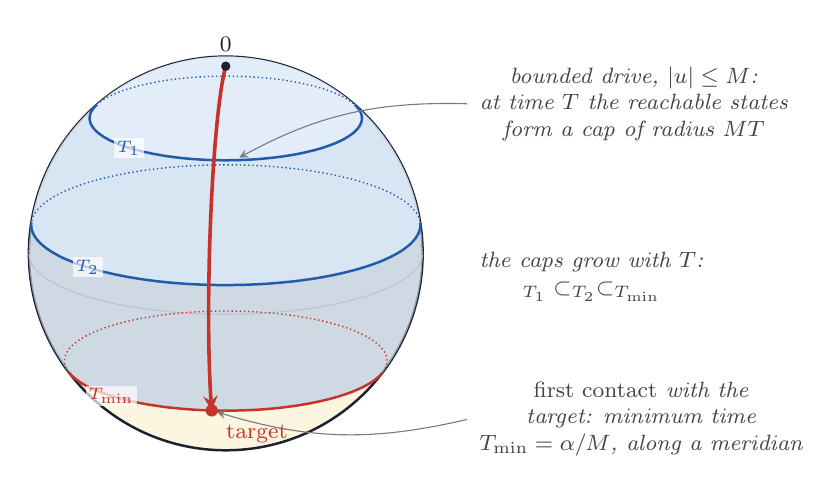
\begin{tikzpicture}[ink/.style={line width=0.9pt, ndInk}, faint/.style={line width=0.4pt, ndInk!35}, dashedink/.style={line width=0.5pt, ndInk!55, dash pattern=on 2.5pt off 2pt}, vec/.style={->, >=stealth, line width=1.2pt}, note/.style={font=\footnotesize\itshape, text=ndInk!85, align=center}, pointer/.style={->, >=stealth, line width=0.4pt, ndInk!60, shorten >=2pt, shorten <=1pt}, dot/.style={circle, fill=ndInk, inner sep=0pt, minimum size=3.4pt}, wash/.style={fill=ndSky, fill opacity=0.55}, every node/.style={text=ndInk}]
\definecolor{ndInk}{rgb}{0.13,0.13,0.18}
\definecolor{ndPaper}{rgb}{0.99,0.96,0.88}
\definecolor{ndSky}{rgb}{0.84,0.91,0.98}
\definecolor{ndRose}{rgb}{0.98,0.86,0.84}
\definecolor{ndBlue}{rgb}{0.13,0.36,0.66}
\definecolor{ndRed}{rgb}{0.78,0.20,0.16}
\definecolor{ndGold}{rgb}{0.88,0.62,0.10}
\definecolor{ndGreen}{rgb}{0.18,0.52,0.30}
\fill[ndPaper] (0.000,0.000) circle (2.500);
\draw[ink] (0.000,0.000) circle (2.500);
\draw[faint] (2.266,-0.326) -- (2.293,-0.308) -- (2.318,-0.289) -- (2.342,-0.271) -- (2.364,-0.252) -- (2.384,-0.232) -- (2.403,-0.213) -- (2.420,-0.193) -- (2.436,-0.174) -- (2.450,-0.154) -- (2.462,-0.134) -- (2.473,-0.114) -- (2.481,-0.094) -- (2.488,-0.074) -- (2.494,-0.054) -- (2.498,-0.034) -- (2.500,-0.013);
\draw[faint] (-2.500,-0.007) -- (-2.498,-0.027) -- (-2.495,-0.047) -- (-2.490,-0.067) -- (-2.484,-0.087) -- (-2.476,-0.108) -- (-2.466,-0.128) -- (-2.454,-0.147) -- (-2.441,-0.167) -- (-2.426,-0.187) -- (-2.409,-0.206) -- (-2.391,-0.226) -- (-2.371,-0.245) -- (-2.349,-0.264) -- (-2.326,-0.283) -- (-2.301,-0.302) -- (-2.275,-0.320) -- (-2.247,-0.339) -- (-2.218,-0.357) -- (-2.187,-0.375) -- (-2.154,-0.392) -- (-2.120,-0.409) -- (-2.085,-0.426) -- (-2.048,-0.443) -- (-2.010,-0.460) -- (-1.970,-0.476) -- (-1.929,-0.491) -- (-1.887,-0.507) -- (-1.843,-0.522) -- (-1.798,-0.537) -- (-1.752,-0.551) -- (-1.705,-0.565) -- (-1.657,-0.579) -- (-1.607,-0.592) -- (-1.556,-0.605) -- (-1.505,-0.617) -- (-1.452,-0.629) -- (-1.398,-0.640) -- (-1.343,-0.652) -- (-1.288,-0.662) -- (-1.231,-0.672) -- (-1.174,-0.682) -- (-1.115,-0.691) -- (-1.057,-0.700) -- (-0.997,-0.708) -- (-0.937,-0.716) -- (-0.876,-0.724) -- (-0.814,-0.730) -- (-0.752,-0.737) -- (-0.689,-0.743) -- (-0.626,-0.748) -- (-0.562,-0.753) -- (-0.498,-0.757) -- (-0.434,-0.761) -- (-0.370,-0.764) -- (-0.305,-0.767) -- (-0.240,-0.769) -- (-0.174,-0.771) -- (-0.109,-0.772) -- (-0.044,-0.772) -- (0.022,-0.773) -- (0.087,-0.772) -- (0.153,-0.771) -- (0.218,-0.770) -- (0.283,-0.768) -- (0.348,-0.765) -- (0.413,-0.762) -- (0.477,-0.758) -- (0.541,-0.754) -- (0.605,-0.750) -- (0.668,-0.744) -- (0.731,-0.739) -- (0.793,-0.733) -- (0.855,-0.726) -- (0.916,-0.719) -- (0.977,-0.711) -- (1.037,-0.703) -- (1.096,-0.694) -- (1.154,-0.685) -- (1.212,-0.676) -- (1.269,-0.666) -- (1.325,-0.655) -- (1.380,-0.644) -- (1.434,-0.633) -- (1.487,-0.621) -- (1.539,-0.609) -- (1.590,-0.596) -- (1.640,-0.583) -- (1.689,-0.570) -- (1.737,-0.556) -- (1.783,-0.541) -- (1.828,-0.527) -- (1.872,-0.512) -- (1.915,-0.497) -- (1.957,-0.481) -- (1.997,-0.465) -- (2.035,-0.449) -- (2.073,-0.432) -- (2.108,-0.415) -- (2.143,-0.398) -- (2.176,-0.380) -- (2.207,-0.363) -- (2.237,-0.345) -- (2.266,-0.326);
\draw[faint, densely dotted] (2.500,0.007) -- (2.498,0.027) -- (2.495,0.047) -- (2.490,0.067) -- (2.484,0.087) -- (2.476,0.108) -- (2.466,0.128) -- (2.454,0.147) -- (2.441,0.167) -- (2.426,0.187) -- (2.409,0.206) -- (2.391,0.226) -- (2.371,0.245) -- (2.349,0.264) -- (2.326,0.283) -- (2.301,0.302) -- (2.275,0.320) -- (2.247,0.339) -- (2.218,0.357) -- (2.187,0.375) -- (2.154,0.392) -- (2.120,0.409) -- (2.085,0.426) -- (2.048,0.443) -- (2.010,0.460) -- (1.970,0.476) -- (1.929,0.491) -- (1.887,0.507) -- (1.843,0.522) -- (1.798,0.537) -- (1.752,0.551) -- (1.705,0.565) -- (1.657,0.579) -- (1.607,0.592) -- (1.556,0.605) -- (1.505,0.617) -- (1.452,0.629) -- (1.398,0.640) -- (1.343,0.652) -- (1.288,0.662) -- (1.231,0.672) -- (1.174,0.682) -- (1.115,0.691) -- (1.057,0.700) -- (0.997,0.708) -- (0.937,0.716) -- (0.876,0.724) -- (0.814,0.730) -- (0.752,0.737) -- (0.689,0.743) -- (0.626,0.748) -- (0.562,0.753) -- (0.498,0.757) -- (0.434,0.761) -- (0.370,0.764) -- (0.305,0.767) -- (0.240,0.769) -- (0.174,0.771) -- (0.109,0.772) -- (0.044,0.772) -- (-0.022,0.773) -- (-0.087,0.772) -- (-0.153,0.771) -- (-0.218,0.770) -- (-0.283,0.768) -- (-0.348,0.765) -- (-0.413,0.762) -- (-0.477,0.758) -- (-0.541,0.754) -- (-0.605,0.750) -- (-0.668,0.744) -- (-0.731,0.739) -- (-0.793,0.733) -- (-0.855,0.726) -- (-0.916,0.719) -- (-0.977,0.711) -- (-1.037,0.703) -- (-1.096,0.694) -- (-1.154,0.685) -- (-1.212,0.676) -- (-1.269,0.666) -- (-1.325,0.655) -- (-1.380,0.644) -- (-1.434,0.633) -- (-1.487,0.621) -- (-1.539,0.609) -- (-1.590,0.596) -- (-1.640,0.583) -- (-1.689,0.570) -- (-1.737,0.556) -- (-1.783,0.541) -- (-1.828,0.527) -- (-1.872,0.512) -- (-1.915,0.497) -- (-1.957,0.481) -- (-1.997,0.465) -- (-2.035,0.449) -- (-2.073,0.432) -- (-2.108,0.415) -- (-2.143,0.398) -- (-2.176,0.380) -- (-2.207,0.363) -- (-2.237,0.345) -- (-2.266,0.326) -- (-2.293,0.308) -- (-2.318,0.289) -- (-2.342,0.271) -- (-2.364,0.252) -- (-2.384,0.232) -- (-2.403,0.213) -- (-2.420,0.193) -- (-2.436,0.174) -- (-2.450,0.154) -- (-2.462,0.134) -- (-2.473,0.114) -- (-2.481,0.094) -- (-2.488,0.074) -- (-2.494,0.054) -- (-2.498,0.034) -- (-2.500,0.013);
\fill[ndBlue!30, fill opacity=0.7] (-1.991,-1.511) -- (-1.987,-1.517) -- (-1.983,-1.522) -- (-1.978,-1.528) -- (-1.973,-1.533) -- (-1.969,-1.538) -- (-1.964,-1.543) -- (-1.958,-1.549) -- (-1.953,-1.554) -- (-1.948,-1.559) -- (-1.942,-1.565) -- (-1.936,-1.570) -- (-1.930,-1.575) -- (-1.924,-1.580) -- (-1.918,-1.585) -- (-1.912,-1.591) -- (-1.905,-1.596) -- (-1.899,-1.601) -- (-1.892,-1.606) -- (-1.885,-1.611) -- (-1.878,-1.616) -- (-1.871,-1.621) -- (-1.863,-1.626) -- (-1.856,-1.631) -- (-1.848,-1.636) -- (-1.841,-1.641) -- (-1.833,-1.646) -- (-1.825,-1.651) -- (-1.816,-1.656) -- (-1.808,-1.661) -- (-1.800,-1.666) -- (-1.791,-1.671) -- (-1.782,-1.675) -- (-1.774,-1.680) -- (-1.765,-1.685) -- (-1.755,-1.690) -- (-1.746,-1.694) -- (-1.737,-1.699) -- (-1.727,-1.704) -- (-1.717,-1.708) -- (-1.708,-1.713) -- (-1.698,-1.718) -- (-1.688,-1.722) -- (-1.678,-1.727) -- (-1.667,-1.731) -- (-1.657,-1.736) -- (-1.646,-1.740) -- (-1.636,-1.745) -- (-1.625,-1.749) -- (-1.614,-1.753) -- (-1.603,-1.758) -- (-1.592,-1.762) -- (-1.580,-1.766) -- (-1.569,-1.771) -- (-1.557,-1.775) -- (-1.546,-1.779) -- (-1.534,-1.783) -- (-1.522,-1.787) -- (-1.510,-1.791) -- (-1.498,-1.795) -- (-1.485,-1.799) -- (-1.473,-1.803) -- (-1.461,-1.807) -- (-1.448,-1.811) -- (-1.435,-1.815) -- (-1.423,-1.819) -- (-1.410,-1.823) -- (-1.397,-1.827) -- (-1.384,-1.830) -- (-1.370,-1.834) -- (-1.357,-1.838) -- (-1.344,-1.841) -- (-1.330,-1.845) -- (-1.316,-1.849) -- (-1.303,-1.852) -- (-1.289,-1.856) -- (-1.275,-1.859) -- (-1.261,-1.862) -- (-1.247,-1.866) -- (-1.232,-1.869) -- (-1.218,-1.872) -- (-1.204,-1.876) -- (-1.189,-1.879) -- (-1.175,-1.882) -- (-1.160,-1.885) -- (-1.145,-1.888) -- (-1.130,-1.891) -- (-1.115,-1.894) -- (-1.100,-1.897) -- (-1.085,-1.900) -- (-1.070,-1.903) -- (-1.055,-1.906) -- (-1.039,-1.909) -- (-1.024,-1.912) -- (-1.008,-1.915) -- (-0.993,-1.917) -- (-0.977,-1.920) -- (-0.961,-1.923) -- (-0.946,-1.925) -- (-0.930,-1.928) -- (-0.914,-1.930) -- (-0.898,-1.933) -- (-0.882,-1.935) -- (-0.865,-1.937) -- (-0.849,-1.940) -- (-0.833,-1.942) -- (-0.817,-1.944) -- (-0.800,-1.946) -- (-0.784,-1.948) -- (-0.767,-1.951) -- (-0.751,-1.953) -- (-0.734,-1.955) -- (-0.717,-1.957) -- (-0.700,-1.958) -- (-0.684,-1.960) -- (-0.667,-1.962) -- (-0.650,-1.964) -- (-0.633,-1.966) -- (-0.616,-1.967) -- (-0.599,-1.969) -- (-0.582,-1.971) -- (-0.564,-1.972) -- (-0.547,-1.974) -- (-0.530,-1.975) -- (-0.513,-1.976) -- (-0.495,-1.978) -- (-0.478,-1.979) -- (-0.461,-1.980) -- (-0.443,-1.982) -- (-0.426,-1.983) -- (-0.408,-1.984) -- (-0.391,-1.985) -- (-0.373,-1.986) -- (-0.356,-1.987) -- (-0.338,-1.988) -- (-0.320,-1.989) -- (-0.303,-1.990) -- (-0.285,-1.990) -- (-0.267,-1.991) -- (-0.250,-1.992) -- (-0.232,-1.993) -- (-0.214,-1.993) -- (-0.196,-1.994) -- (-0.178,-1.994) -- (-0.161,-1.995) -- (-0.143,-1.995) -- (-0.125,-1.995) -- (-0.107,-1.996) -- (-0.089,-1.996) -- (-0.071,-1.996) -- (-0.054,-1.996) -- (-0.036,-1.996) -- (-0.018,-1.997) -- (-0.000,-1.997) -- (0.018,-1.997) -- (0.036,-1.996) -- (0.054,-1.996) -- (0.071,-1.996) -- (0.089,-1.996) -- (0.107,-1.996) -- (0.125,-1.995) -- (0.143,-1.995) -- (0.161,-1.995) -- (0.178,-1.994) -- (0.196,-1.994) -- (0.214,-1.993) -- (0.232,-1.993) -- (0.250,-1.992) -- (0.267,-1.991) -- (0.285,-1.990) -- (0.303,-1.990) -- (0.320,-1.989) -- (0.338,-1.988) -- (0.356,-1.987) -- (0.373,-1.986) -- (0.391,-1.985) -- (0.408,-1.984) -- (0.426,-1.983) -- (0.443,-1.982) -- (0.461,-1.980) -- (0.478,-1.979) -- (0.495,-1.978) -- (0.513,-1.976) -- (0.530,-1.975) -- (0.547,-1.974) -- (0.564,-1.972) -- (0.582,-1.971) -- (0.599,-1.969) -- (0.616,-1.967) -- (0.633,-1.966) -- (0.650,-1.964) -- (0.667,-1.962) -- (0.684,-1.960) -- (0.700,-1.958) -- (0.717,-1.957) -- (0.734,-1.955) -- (0.751,-1.953) -- (0.767,-1.951) -- (0.784,-1.948) -- (0.800,-1.946) -- (0.817,-1.944) -- (0.833,-1.942) -- (0.849,-1.940) -- (0.865,-1.937) -- (0.882,-1.935) -- (0.898,-1.933) -- (0.914,-1.930) -- (0.930,-1.928) -- (0.946,-1.925) -- (0.961,-1.923) -- (0.977,-1.920) -- (0.993,-1.917) -- (1.008,-1.915) -- (1.024,-1.912) -- (1.039,-1.909) -- (1.055,-1.906) -- (1.070,-1.903) -- (1.085,-1.900) -- (1.100,-1.897) -- (1.115,-1.894) -- (1.130,-1.891) -- (1.145,-1.888) -- (1.160,-1.885) -- (1.175,-1.882) -- (1.189,-1.879) -- (1.204,-1.876) -- (1.218,-1.872) -- (1.232,-1.869) -- (1.247,-1.866) -- (1.261,-1.862) -- (1.275,-1.859) -- (1.289,-1.856) -- (1.303,-1.852) -- (1.316,-1.849) -- (1.330,-1.845) -- (1.344,-1.841) -- (1.357,-1.838) -- (1.370,-1.834) -- (1.384,-1.830) -- (1.397,-1.827) -- (1.410,-1.823) -- (1.423,-1.819) -- (1.435,-1.815) -- (1.448,-1.811) -- (1.461,-1.807) -- (1.473,-1.803) -- (1.485,-1.799) -- (1.498,-1.795) -- (1.510,-1.791) -- (1.522,-1.787) -- (1.534,-1.783) -- (1.546,-1.779) -- (1.557,-1.775) -- (1.569,-1.771) -- (1.580,-1.766) -- (1.592,-1.762) -- (1.603,-1.758) -- (1.614,-1.753) -- (1.625,-1.749) -- (1.636,-1.745) -- (1.646,-1.740) -- (1.657,-1.736) -- (1.667,-1.731) -- (1.678,-1.727) -- (1.688,-1.722) -- (1.698,-1.718) -- (1.708,-1.713) -- (1.717,-1.708) -- (1.727,-1.704) -- (1.737,-1.699) -- (1.746,-1.694) -- (1.755,-1.690) -- (1.765,-1.685) -- (1.774,-1.680) -- (1.782,-1.675) -- (1.791,-1.671) -- (1.800,-1.666) -- (1.808,-1.661) -- (1.816,-1.656) -- (1.825,-1.651) -- (1.833,-1.646) -- (1.841,-1.641) -- (1.848,-1.636) -- (1.856,-1.631) -- (1.863,-1.626) -- (1.871,-1.621) -- (1.878,-1.616) -- (1.885,-1.611) -- (1.892,-1.606) -- (1.899,-1.601) -- (1.905,-1.596) -- (1.912,-1.591) -- (1.918,-1.585) -- (1.924,-1.580) -- (1.930,-1.575) -- (1.936,-1.570) -- (1.942,-1.565) -- (1.948,-1.559) -- (1.953,-1.554) -- (1.958,-1.549) -- (1.964,-1.543) -- (1.969,-1.538) -- (1.973,-1.533) -- (1.978,-1.528) -- (1.983,-1.522) -- (1.987,-1.517) -- (1.991,-1.511) -- (1.997,-1.505) -- (2.010,-1.487) -- (2.023,-1.469) -- (2.035,-1.452) -- (2.048,-1.434) -- (2.060,-1.416) -- (2.073,-1.398) -- (2.085,-1.380) -- (2.097,-1.362) -- (2.108,-1.343) -- (2.120,-1.325) -- (2.132,-1.306) -- (2.143,-1.288) -- (2.154,-1.269) -- (2.165,-1.250) -- (2.176,-1.231) -- (2.187,-1.212) -- (2.197,-1.193) -- (2.207,-1.174) -- (2.218,-1.154) -- (2.228,-1.135) -- (2.237,-1.115) -- (2.247,-1.096) -- (2.256,-1.076) -- (2.266,-1.057) -- (2.275,-1.037) -- (2.284,-1.017) -- (2.293,-0.997) -- (2.301,-0.977) -- (2.310,-0.957) -- (2.318,-0.937) -- (2.326,-0.916) -- (2.334,-0.896) -- (2.342,-0.876) -- (2.349,-0.855) -- (2.357,-0.835) -- (2.364,-0.814) -- (2.371,-0.793) -- (2.378,-0.773) -- (2.384,-0.752) -- (2.391,-0.731) -- (2.397,-0.710) -- (2.403,-0.689) -- (2.409,-0.668) -- (2.415,-0.647) -- (2.420,-0.626) -- (2.426,-0.605) -- (2.431,-0.584) -- (2.436,-0.562) -- (2.441,-0.541) -- (2.445,-0.520) -- (2.450,-0.498) -- (2.454,-0.477) -- (2.458,-0.456) -- (2.462,-0.434) -- (2.466,-0.413) -- (2.469,-0.391) -- (2.473,-0.370) -- (2.476,-0.348) -- (2.479,-0.326) -- (2.481,-0.305) -- (2.484,-0.283) -- (2.486,-0.261) -- (2.488,-0.240) -- (2.490,-0.218) -- (2.492,-0.196) -- (2.494,-0.174) -- (2.495,-0.153) -- (2.497,-0.131) -- (2.498,-0.109) -- (2.498,-0.087) -- (2.499,-0.065) -- (2.500,-0.044) -- (2.500,-0.022) -- (2.500,0.000) -- (2.500,0.022) -- (2.500,0.044) -- (2.499,0.065) -- (2.498,0.087) -- (2.498,0.109) -- (2.497,0.131) -- (2.495,0.153) -- (2.494,0.174) -- (2.492,0.196) -- (2.490,0.218) -- (2.488,0.240) -- (2.486,0.261) -- (2.484,0.283) -- (2.481,0.305) -- (2.479,0.326) -- (2.476,0.348) -- (2.473,0.370) -- (2.469,0.391) -- (2.466,0.413) -- (2.462,0.434) -- (2.458,0.456) -- (2.454,0.477) -- (2.450,0.498) -- (2.445,0.520) -- (2.441,0.541) -- (2.436,0.562) -- (2.431,0.584) -- (2.426,0.605) -- (2.420,0.626) -- (2.415,0.647) -- (2.409,0.668) -- (2.403,0.689) -- (2.397,0.710) -- (2.391,0.731) -- (2.384,0.752) -- (2.378,0.773) -- (2.371,0.793) -- (2.364,0.814) -- (2.357,0.835) -- (2.349,0.855) -- (2.342,0.876) -- (2.334,0.896) -- (2.326,0.916) -- (2.318,0.937) -- (2.310,0.957) -- (2.301,0.977) -- (2.293,0.997) -- (2.284,1.017) -- (2.275,1.037) -- (2.266,1.057) -- (2.256,1.076) -- (2.247,1.096) -- (2.237,1.115) -- (2.228,1.135) -- (2.218,1.154) -- (2.207,1.174) -- (2.197,1.193) -- (2.187,1.212) -- (2.176,1.231) -- (2.165,1.250) -- (2.154,1.269) -- (2.143,1.288) -- (2.132,1.306) -- (2.120,1.325) -- (2.108,1.343) -- (2.097,1.362) -- (2.085,1.380) -- (2.073,1.398) -- (2.060,1.416) -- (2.048,1.434) -- (2.035,1.452) -- (2.023,1.469) -- (2.010,1.487) -- (1.997,1.505) -- (1.983,1.522) -- (1.970,1.539) -- (1.957,1.556) -- (1.943,1.573) -- (1.929,1.590) -- (1.915,1.607) -- (1.901,1.624) -- (1.887,1.640) -- (1.872,1.657) -- (1.858,1.673) -- (1.843,1.689) -- (1.828,1.705) -- (1.813,1.721) -- (1.798,1.737) -- (1.783,1.752) -- (1.768,1.768) -- (1.752,1.783) -- (1.737,1.798) -- (1.721,1.813) -- (1.705,1.828) -- (1.689,1.843) -- (1.673,1.858) -- (1.657,1.872) -- (1.640,1.887) -- (1.624,1.901) -- (1.607,1.915) -- (1.590,1.929) -- (1.573,1.943) -- (1.556,1.957) -- (1.539,1.970) -- (1.522,1.983) -- (1.505,1.997) -- (1.487,2.010) -- (1.469,2.023) -- (1.452,2.035) -- (1.434,2.048) -- (1.416,2.060) -- (1.398,2.073) -- (1.380,2.085) -- (1.362,2.097) -- (1.343,2.108) -- (1.325,2.120) -- (1.306,2.132) -- (1.288,2.143) -- (1.269,2.154) -- (1.250,2.165) -- (1.231,2.176) -- (1.212,2.187) -- (1.193,2.197) -- (1.174,2.207) -- (1.154,2.218) -- (1.135,2.228) -- (1.115,2.237) -- (1.096,2.247) -- (1.076,2.256) -- (1.057,2.266) -- (1.037,2.275) -- (1.017,2.284) -- (0.997,2.293) -- (0.977,2.301) -- (0.957,2.310) -- (0.937,2.318) -- (0.916,2.326) -- (0.896,2.334) -- (0.876,2.342) -- (0.855,2.349) -- (0.835,2.357) -- (0.814,2.364) -- (0.793,2.371) -- (0.773,2.378) -- (0.752,2.384) -- (0.731,2.391) -- (0.710,2.397) -- (0.689,2.403) -- (0.668,2.409) -- (0.647,2.415) -- (0.626,2.420) -- (0.605,2.426) -- (0.584,2.431) -- (0.562,2.436) -- (0.541,2.441) -- (0.520,2.445) -- (0.498,2.450) -- (0.477,2.454) -- (0.456,2.458) -- (0.434,2.462) -- (0.413,2.466) -- (0.391,2.469) -- (0.370,2.473) -- (0.348,2.476) -- (0.326,2.479) -- (0.305,2.481) -- (0.283,2.484) -- (0.261,2.486) -- (0.240,2.488) -- (0.218,2.490) -- (0.196,2.492) -- (0.174,2.494) -- (0.153,2.495) -- (0.131,2.497) -- (0.109,2.498) -- (0.087,2.498) -- (0.065,2.499) -- (0.044,2.500) -- (0.022,2.500) -- (0.000,2.500) -- (-0.022,2.500) -- (-0.044,2.500) -- (-0.065,2.499) -- (-0.087,2.498) -- (-0.109,2.498) -- (-0.131,2.497) -- (-0.153,2.495) -- (-0.174,2.494) -- (-0.196,2.492) -- (-0.218,2.490) -- (-0.240,2.488) -- (-0.261,2.486) -- (-0.283,2.484) -- (-0.305,2.481) -- (-0.326,2.479) -- (-0.348,2.476) -- (-0.370,2.473) -- (-0.391,2.469) -- (-0.413,2.466) -- (-0.434,2.462) -- (-0.456,2.458) -- (-0.477,2.454) -- (-0.498,2.450) -- (-0.520,2.445) -- (-0.541,2.441) -- (-0.562,2.436) -- (-0.584,2.431) -- (-0.605,2.426) -- (-0.626,2.420) -- (-0.647,2.415) -- (-0.668,2.409) -- (-0.689,2.403) -- (-0.710,2.397) -- (-0.731,2.391) -- (-0.752,2.384) -- (-0.773,2.378) -- (-0.793,2.371) -- (-0.814,2.364) -- (-0.835,2.357) -- (-0.855,2.349) -- (-0.876,2.342) -- (-0.896,2.334) -- (-0.916,2.326) -- (-0.937,2.318) -- (-0.957,2.310) -- (-0.977,2.301) -- (-0.997,2.293) -- (-1.017,2.284) -- (-1.037,2.275) -- (-1.057,2.266) -- (-1.076,2.256) -- (-1.096,2.247) -- (-1.115,2.237) -- (-1.135,2.228) -- (-1.154,2.218) -- (-1.174,2.207) -- (-1.193,2.197) -- (-1.212,2.187) -- (-1.231,2.176) -- (-1.250,2.165) -- (-1.269,2.154) -- (-1.288,2.143) -- (-1.306,2.132) -- (-1.325,2.120) -- (-1.343,2.108) -- (-1.362,2.097) -- (-1.380,2.085) -- (-1.398,2.073) -- (-1.416,2.060) -- (-1.434,2.048) -- (-1.452,2.035) -- (-1.469,2.023) -- (-1.487,2.010) -- (-1.505,1.997) -- (-1.522,1.983) -- (-1.539,1.970) -- (-1.556,1.957) -- (-1.573,1.943) -- (-1.590,1.929) -- (-1.607,1.915) -- (-1.624,1.901) -- (-1.640,1.887) -- (-1.657,1.872) -- (-1.673,1.858) -- (-1.689,1.843) -- (-1.705,1.828) -- (-1.721,1.813) -- (-1.737,1.798) -- (-1.752,1.783) -- (-1.768,1.768) -- (-1.783,1.752) -- (-1.798,1.737) -- (-1.813,1.721) -- (-1.828,1.705) -- (-1.843,1.689) -- (-1.858,1.673) -- (-1.872,1.657) -- (-1.887,1.640) -- (-1.901,1.624) -- (-1.915,1.607) -- (-1.929,1.590) -- (-1.943,1.573) -- (-1.957,1.556) -- (-1.970,1.539) -- (-1.983,1.522) -- (-1.997,1.505) -- (-2.010,1.487) -- (-2.023,1.469) -- (-2.035,1.452) -- (-2.048,1.434) -- (-2.060,1.416) -- (-2.073,1.398) -- (-2.085,1.380) -- (-2.097,1.362) -- (-2.108,1.343) -- (-2.120,1.325) -- (-2.132,1.306) -- (-2.143,1.288) -- (-2.154,1.269) -- (-2.165,1.250) -- (-2.176,1.231) -- (-2.187,1.212) -- (-2.197,1.193) -- (-2.207,1.174) -- (-2.218,1.154) -- (-2.228,1.135) -- (-2.237,1.115) -- (-2.247,1.096) -- (-2.256,1.076) -- (-2.266,1.057) -- (-2.275,1.037) -- (-2.284,1.017) -- (-2.293,0.997) -- (-2.301,0.977) -- (-2.310,0.957) -- (-2.318,0.937) -- (-2.326,0.916) -- (-2.334,0.896) -- (-2.342,0.876) -- (-2.349,0.855) -- (-2.357,0.835) -- (-2.364,0.814) -- (-2.371,0.793) -- (-2.378,0.773) -- (-2.384,0.752) -- (-2.391,0.731) -- (-2.397,0.710) -- (-2.403,0.689) -- (-2.409,0.668) -- (-2.415,0.647) -- (-2.420,0.626) -- (-2.426,0.605) -- (-2.431,0.584) -- (-2.436,0.562) -- (-2.441,0.541) -- (-2.445,0.520) -- (-2.450,0.498) -- (-2.454,0.477) -- (-2.458,0.456) -- (-2.462,0.434) -- (-2.466,0.413) -- (-2.469,0.391) -- (-2.473,0.370) -- (-2.476,0.348) -- (-2.479,0.326) -- (-2.481,0.305) -- (-2.484,0.283) -- (-2.486,0.261) -- (-2.488,0.240) -- (-2.490,0.218) -- (-2.492,0.196) -- (-2.494,0.174) -- (-2.495,0.153) -- (-2.497,0.131) -- (-2.498,0.109) -- (-2.498,0.087) -- (-2.499,0.065) -- (-2.500,0.044) -- (-2.500,0.022) -- (-2.500,0.000) -- (-2.500,-0.022) -- (-2.500,-0.044) -- (-2.499,-0.065) -- (-2.498,-0.087) -- (-2.498,-0.109) -- (-2.497,-0.131) -- (-2.495,-0.153) -- (-2.494,-0.174) -- (-2.492,-0.196) -- (-2.490,-0.218) -- (-2.488,-0.240) -- (-2.486,-0.261) -- (-2.484,-0.283) -- (-2.481,-0.305) -- (-2.479,-0.326) -- (-2.476,-0.348) -- (-2.473,-0.370) -- (-2.469,-0.391) -- (-2.466,-0.413) -- (-2.462,-0.434) -- (-2.458,-0.456) -- (-2.454,-0.477) -- (-2.450,-0.498) -- (-2.445,-0.520) -- (-2.441,-0.541) -- (-2.436,-0.562) -- (-2.431,-0.584) -- (-2.426,-0.605) -- (-2.420,-0.626) -- (-2.415,-0.647) -- (-2.409,-0.668) -- (-2.403,-0.689) -- (-2.397,-0.710) -- (-2.391,-0.731) -- (-2.384,-0.752) -- (-2.378,-0.773) -- (-2.371,-0.793) -- (-2.364,-0.814) -- (-2.357,-0.835) -- (-2.349,-0.855) -- (-2.342,-0.876) -- (-2.334,-0.896) -- (-2.326,-0.916) -- (-2.318,-0.937) -- (-2.310,-0.957) -- (-2.301,-0.977) -- (-2.293,-0.997) -- (-2.284,-1.017) -- (-2.275,-1.037) -- (-2.266,-1.057) -- (-2.256,-1.076) -- (-2.247,-1.096) -- (-2.237,-1.115) -- (-2.228,-1.135) -- (-2.218,-1.154) -- (-2.207,-1.174) -- (-2.197,-1.193) -- (-2.187,-1.212) -- (-2.176,-1.231) -- (-2.165,-1.250) -- (-2.154,-1.269) -- (-2.143,-1.288) -- (-2.132,-1.306) -- (-2.120,-1.325) -- (-2.108,-1.343) -- (-2.097,-1.362) -- (-2.085,-1.380) -- (-2.073,-1.398) -- (-2.060,-1.416) -- (-2.048,-1.434) -- (-2.035,-1.452) -- (-2.023,-1.469) -- (-2.010,-1.487) -- (-1.997,-1.505) -- cycle;
\fill[ndSky!85, fill opacity=0.7] (-2.469,0.395) -- (-2.469,0.388) -- (-2.470,0.382) -- (-2.471,0.375) -- (-2.471,0.368) -- (-2.471,0.362) -- (-2.471,0.355) -- (-2.471,0.348) -- (-2.470,0.342) -- (-2.469,0.335) -- (-2.469,0.328) -- (-2.468,0.322) -- (-2.466,0.315) -- (-2.465,0.308) -- (-2.463,0.302) -- (-2.462,0.295) -- (-2.460,0.289) -- (-2.457,0.282) -- (-2.455,0.275) -- (-2.452,0.269) -- (-2.450,0.262) -- (-2.447,0.255) -- (-2.444,0.249) -- (-2.440,0.242) -- (-2.437,0.236) -- (-2.433,0.229) -- (-2.430,0.223) -- (-2.426,0.216) -- (-2.421,0.209) -- (-2.417,0.203) -- (-2.412,0.196) -- (-2.408,0.190) -- (-2.403,0.183) -- (-2.398,0.177) -- (-2.392,0.171) -- (-2.387,0.164) -- (-2.381,0.158) -- (-2.375,0.151) -- (-2.369,0.145) -- (-2.363,0.138) -- (-2.357,0.132) -- (-2.350,0.126) -- (-2.343,0.119) -- (-2.336,0.113) -- (-2.329,0.107) -- (-2.322,0.101) -- (-2.314,0.094) -- (-2.307,0.088) -- (-2.299,0.082) -- (-2.291,0.076) -- (-2.283,0.069) -- (-2.274,0.063) -- (-2.266,0.057) -- (-2.257,0.051) -- (-2.248,0.045) -- (-2.239,0.039) -- (-2.230,0.033) -- (-2.221,0.027) -- (-2.211,0.021) -- (-2.202,0.015) -- (-2.192,0.009) -- (-2.182,0.003) -- (-2.171,-0.003) -- (-2.161,-0.008) -- (-2.151,-0.014) -- (-2.140,-0.020) -- (-2.129,-0.026) -- (-2.118,-0.032) -- (-2.107,-0.037) -- (-2.095,-0.043) -- (-2.084,-0.049) -- (-2.072,-0.054) -- (-2.060,-0.060) -- (-2.048,-0.065) -- (-2.036,-0.071) -- (-2.024,-0.076) -- (-2.012,-0.082) -- (-1.999,-0.087) -- (-1.986,-0.092) -- (-1.973,-0.098) -- (-1.960,-0.103) -- (-1.947,-0.108) -- (-1.934,-0.114) -- (-1.920,-0.119) -- (-1.907,-0.124) -- (-1.893,-0.129) -- (-1.879,-0.134) -- (-1.865,-0.139) -- (-1.851,-0.144) -- (-1.836,-0.149) -- (-1.822,-0.154) -- (-1.807,-0.159) -- (-1.792,-0.164) -- (-1.777,-0.169) -- (-1.762,-0.173) -- (-1.747,-0.178) -- (-1.732,-0.183) -- (-1.716,-0.188) -- (-1.701,-0.192) -- (-1.685,-0.197) -- (-1.669,-0.201) -- (-1.653,-0.206) -- (-1.637,-0.210) -- (-1.621,-0.215) -- (-1.605,-0.219) -- (-1.588,-0.223) -- (-1.572,-0.227) -- (-1.555,-0.232) -- (-1.538,-0.236) -- (-1.521,-0.240) -- (-1.504,-0.244) -- (-1.487,-0.248) -- (-1.470,-0.252) -- (-1.452,-0.256) -- (-1.435,-0.260) -- (-1.417,-0.264) -- (-1.400,-0.268) -- (-1.382,-0.271) -- (-1.364,-0.275) -- (-1.346,-0.279) -- (-1.328,-0.282) -- (-1.309,-0.286) -- (-1.291,-0.289) -- (-1.273,-0.293) -- (-1.254,-0.296) -- (-1.235,-0.300) -- (-1.217,-0.303) -- (-1.198,-0.306) -- (-1.179,-0.309) -- (-1.160,-0.312) -- (-1.141,-0.316) -- (-1.122,-0.319) -- (-1.103,-0.322) -- (-1.083,-0.325) -- (-1.064,-0.327) -- (-1.044,-0.330) -- (-1.025,-0.333) -- (-1.005,-0.336) -- (-0.985,-0.339) -- (-0.965,-0.341) -- (-0.946,-0.344) -- (-0.926,-0.346) -- (-0.906,-0.349) -- (-0.885,-0.351) -- (-0.865,-0.354) -- (-0.845,-0.356) -- (-0.825,-0.358) -- (-0.804,-0.360) -- (-0.784,-0.362) -- (-0.764,-0.364) -- (-0.743,-0.367) -- (-0.722,-0.368) -- (-0.702,-0.370) -- (-0.681,-0.372) -- (-0.660,-0.374) -- (-0.640,-0.376) -- (-0.619,-0.378) -- (-0.598,-0.379) -- (-0.577,-0.381) -- (-0.556,-0.382) -- (-0.535,-0.384) -- (-0.514,-0.385) -- (-0.493,-0.387) -- (-0.471,-0.388) -- (-0.450,-0.389) -- (-0.429,-0.390) -- (-0.408,-0.391) -- (-0.387,-0.392) -- (-0.365,-0.393) -- (-0.344,-0.394) -- (-0.323,-0.395) -- (-0.301,-0.396) -- (-0.280,-0.397) -- (-0.258,-0.398) -- (-0.237,-0.398) -- (-0.215,-0.399) -- (-0.194,-0.400) -- (-0.172,-0.400) -- (-0.151,-0.400) -- (-0.129,-0.401) -- (-0.108,-0.401) -- (-0.086,-0.401) -- (-0.065,-0.402) -- (-0.043,-0.402) -- (-0.022,-0.402) -- (0.000,-0.402) -- (0.022,-0.402) -- (0.043,-0.402) -- (0.065,-0.402) -- (0.086,-0.401) -- (0.108,-0.401) -- (0.129,-0.401) -- (0.151,-0.400) -- (0.172,-0.400) -- (0.194,-0.400) -- (0.215,-0.399) -- (0.237,-0.398) -- (0.258,-0.398) -- (0.280,-0.397) -- (0.301,-0.396) -- (0.323,-0.395) -- (0.344,-0.394) -- (0.365,-0.393) -- (0.387,-0.392) -- (0.408,-0.391) -- (0.429,-0.390) -- (0.450,-0.389) -- (0.471,-0.388) -- (0.493,-0.387) -- (0.514,-0.385) -- (0.535,-0.384) -- (0.556,-0.382) -- (0.577,-0.381) -- (0.598,-0.379) -- (0.619,-0.378) -- (0.640,-0.376) -- (0.660,-0.374) -- (0.681,-0.372) -- (0.702,-0.370) -- (0.722,-0.368) -- (0.743,-0.367) -- (0.764,-0.364) -- (0.784,-0.362) -- (0.804,-0.360) -- (0.825,-0.358) -- (0.845,-0.356) -- (0.865,-0.354) -- (0.885,-0.351) -- (0.906,-0.349) -- (0.926,-0.346) -- (0.946,-0.344) -- (0.965,-0.341) -- (0.985,-0.339) -- (1.005,-0.336) -- (1.025,-0.333) -- (1.044,-0.330) -- (1.064,-0.327) -- (1.083,-0.325) -- (1.103,-0.322) -- (1.122,-0.319) -- (1.141,-0.316) -- (1.160,-0.312) -- (1.179,-0.309) -- (1.198,-0.306) -- (1.217,-0.303) -- (1.235,-0.300) -- (1.254,-0.296) -- (1.273,-0.293) -- (1.291,-0.289) -- (1.309,-0.286) -- (1.328,-0.282) -- (1.346,-0.279) -- (1.364,-0.275) -- (1.382,-0.271) -- (1.400,-0.268) -- (1.417,-0.264) -- (1.435,-0.260) -- (1.452,-0.256) -- (1.470,-0.252) -- (1.487,-0.248) -- (1.504,-0.244) -- (1.521,-0.240) -- (1.538,-0.236) -- (1.555,-0.232) -- (1.572,-0.227) -- (1.588,-0.223) -- (1.605,-0.219) -- (1.621,-0.215) -- (1.637,-0.210) -- (1.653,-0.206) -- (1.669,-0.201) -- (1.685,-0.197) -- (1.701,-0.192) -- (1.716,-0.188) -- (1.732,-0.183) -- (1.747,-0.178) -- (1.762,-0.173) -- (1.777,-0.169) -- (1.792,-0.164) -- (1.807,-0.159) -- (1.822,-0.154) -- (1.836,-0.149) -- (1.851,-0.144) -- (1.865,-0.139) -- (1.879,-0.134) -- (1.893,-0.129) -- (1.907,-0.124) -- (1.920,-0.119) -- (1.934,-0.114) -- (1.947,-0.108) -- (1.960,-0.103) -- (1.973,-0.098) -- (1.986,-0.092) -- (1.999,-0.087) -- (2.012,-0.082) -- (2.024,-0.076) -- (2.036,-0.071) -- (2.048,-0.065) -- (2.060,-0.060) -- (2.072,-0.054) -- (2.084,-0.049) -- (2.095,-0.043) -- (2.107,-0.037) -- (2.118,-0.032) -- (2.129,-0.026) -- (2.140,-0.020) -- (2.151,-0.014) -- (2.161,-0.008) -- (2.171,-0.003) -- (2.182,0.003) -- (2.192,0.009) -- (2.202,0.015) -- (2.211,0.021) -- (2.221,0.027) -- (2.230,0.033) -- (2.239,0.039) -- (2.248,0.045) -- (2.257,0.051) -- (2.266,0.057) -- (2.274,0.063) -- (2.283,0.069) -- (2.291,0.076) -- (2.299,0.082) -- (2.307,0.088) -- (2.314,0.094) -- (2.322,0.101) -- (2.329,0.107) -- (2.336,0.113) -- (2.343,0.119) -- (2.350,0.126) -- (2.357,0.132) -- (2.363,0.138) -- (2.369,0.145) -- (2.375,0.151) -- (2.381,0.158) -- (2.387,0.164) -- (2.392,0.171) -- (2.398,0.177) -- (2.403,0.183) -- (2.408,0.190) -- (2.412,0.196) -- (2.417,0.203) -- (2.421,0.209) -- (2.426,0.216) -- (2.430,0.223) -- (2.433,0.229) -- (2.437,0.236) -- (2.440,0.242) -- (2.444,0.249) -- (2.447,0.255) -- (2.450,0.262) -- (2.452,0.269) -- (2.455,0.275) -- (2.457,0.282) -- (2.460,0.289) -- (2.462,0.295) -- (2.463,0.302) -- (2.465,0.308) -- (2.466,0.315) -- (2.468,0.322) -- (2.469,0.328) -- (2.469,0.335) -- (2.470,0.342) -- (2.471,0.348) -- (2.471,0.355) -- (2.471,0.362) -- (2.471,0.368) -- (2.471,0.375) -- (2.470,0.382) -- (2.469,0.388) -- (2.469,0.395) -- (2.466,0.413) -- (2.462,0.434) -- (2.458,0.456) -- (2.454,0.477) -- (2.450,0.498) -- (2.445,0.520) -- (2.441,0.541) -- (2.436,0.562) -- (2.431,0.584) -- (2.426,0.605) -- (2.420,0.626) -- (2.415,0.647) -- (2.409,0.668) -- (2.403,0.689) -- (2.397,0.710) -- (2.391,0.731) -- (2.384,0.752) -- (2.378,0.773) -- (2.371,0.793) -- (2.364,0.814) -- (2.357,0.835) -- (2.349,0.855) -- (2.342,0.876) -- (2.334,0.896) -- (2.326,0.916) -- (2.318,0.937) -- (2.310,0.957) -- (2.301,0.977) -- (2.293,0.997) -- (2.284,1.017) -- (2.275,1.037) -- (2.266,1.057) -- (2.256,1.076) -- (2.247,1.096) -- (2.237,1.115) -- (2.228,1.135) -- (2.218,1.154) -- (2.207,1.174) -- (2.197,1.193) -- (2.187,1.212) -- (2.176,1.231) -- (2.165,1.250) -- (2.154,1.269) -- (2.143,1.288) -- (2.132,1.306) -- (2.120,1.325) -- (2.108,1.343) -- (2.097,1.362) -- (2.085,1.380) -- (2.073,1.398) -- (2.060,1.416) -- (2.048,1.434) -- (2.035,1.452) -- (2.023,1.469) -- (2.010,1.487) -- (1.997,1.505) -- (1.983,1.522) -- (1.970,1.539) -- (1.957,1.556) -- (1.943,1.573) -- (1.929,1.590) -- (1.915,1.607) -- (1.901,1.624) -- (1.887,1.640) -- (1.872,1.657) -- (1.858,1.673) -- (1.843,1.689) -- (1.828,1.705) -- (1.813,1.721) -- (1.798,1.737) -- (1.783,1.752) -- (1.768,1.768) -- (1.752,1.783) -- (1.737,1.798) -- (1.721,1.813) -- (1.705,1.828) -- (1.689,1.843) -- (1.673,1.858) -- (1.657,1.872) -- (1.640,1.887) -- (1.624,1.901) -- (1.607,1.915) -- (1.590,1.929) -- (1.573,1.943) -- (1.556,1.957) -- (1.539,1.970) -- (1.522,1.983) -- (1.505,1.997) -- (1.487,2.010) -- (1.469,2.023) -- (1.452,2.035) -- (1.434,2.048) -- (1.416,2.060) -- (1.398,2.073) -- (1.380,2.085) -- (1.362,2.097) -- (1.343,2.108) -- (1.325,2.120) -- (1.306,2.132) -- (1.288,2.143) -- (1.269,2.154) -- (1.250,2.165) -- (1.231,2.176) -- (1.212,2.187) -- (1.193,2.197) -- (1.174,2.207) -- (1.154,2.218) -- (1.135,2.228) -- (1.115,2.237) -- (1.096,2.247) -- (1.076,2.256) -- (1.057,2.266) -- (1.037,2.275) -- (1.017,2.284) -- (0.997,2.293) -- (0.977,2.301) -- (0.957,2.310) -- (0.937,2.318) -- (0.916,2.326) -- (0.896,2.334) -- (0.876,2.342) -- (0.855,2.349) -- (0.835,2.357) -- (0.814,2.364) -- (0.793,2.371) -- (0.773,2.378) -- (0.752,2.384) -- (0.731,2.391) -- (0.710,2.397) -- (0.689,2.403) -- (0.668,2.409) -- (0.647,2.415) -- (0.626,2.420) -- (0.605,2.426) -- (0.584,2.431) -- (0.562,2.436) -- (0.541,2.441) -- (0.520,2.445) -- (0.498,2.450) -- (0.477,2.454) -- (0.456,2.458) -- (0.434,2.462) -- (0.413,2.466) -- (0.391,2.469) -- (0.370,2.473) -- (0.348,2.476) -- (0.326,2.479) -- (0.305,2.481) -- (0.283,2.484) -- (0.261,2.486) -- (0.240,2.488) -- (0.218,2.490) -- (0.196,2.492) -- (0.174,2.494) -- (0.153,2.495) -- (0.131,2.497) -- (0.109,2.498) -- (0.087,2.498) -- (0.065,2.499) -- (0.044,2.500) -- (0.022,2.500) -- (0.000,2.500) -- (-0.022,2.500) -- (-0.044,2.500) -- (-0.065,2.499) -- (-0.087,2.498) -- (-0.109,2.498) -- (-0.131,2.497) -- (-0.153,2.495) -- (-0.174,2.494) -- (-0.196,2.492) -- (-0.218,2.490) -- (-0.240,2.488) -- (-0.261,2.486) -- (-0.283,2.484) -- (-0.305,2.481) -- (-0.326,2.479) -- (-0.348,2.476) -- (-0.370,2.473) -- (-0.391,2.469) -- (-0.413,2.466) -- (-0.434,2.462) -- (-0.456,2.458) -- (-0.477,2.454) -- (-0.498,2.450) -- (-0.520,2.445) -- (-0.541,2.441) -- (-0.562,2.436) -- (-0.584,2.431) -- (-0.605,2.426) -- (-0.626,2.420) -- (-0.647,2.415) -- (-0.668,2.409) -- (-0.689,2.403) -- (-0.710,2.397) -- (-0.731,2.391) -- (-0.752,2.384) -- (-0.773,2.378) -- (-0.793,2.371) -- (-0.814,2.364) -- (-0.835,2.357) -- (-0.855,2.349) -- (-0.876,2.342) -- (-0.896,2.334) -- (-0.916,2.326) -- (-0.937,2.318) -- (-0.957,2.310) -- (-0.977,2.301) -- (-0.997,2.293) -- (-1.017,2.284) -- (-1.037,2.275) -- (-1.057,2.266) -- (-1.076,2.256) -- (-1.096,2.247) -- (-1.115,2.237) -- (-1.135,2.228) -- (-1.154,2.218) -- (-1.174,2.207) -- (-1.193,2.197) -- (-1.212,2.187) -- (-1.231,2.176) -- (-1.250,2.165) -- (-1.269,2.154) -- (-1.288,2.143) -- (-1.306,2.132) -- (-1.325,2.120) -- (-1.343,2.108) -- (-1.362,2.097) -- (-1.380,2.085) -- (-1.398,2.073) -- (-1.416,2.060) -- (-1.434,2.048) -- (-1.452,2.035) -- (-1.469,2.023) -- (-1.487,2.010) -- (-1.505,1.997) -- (-1.522,1.983) -- (-1.539,1.970) -- (-1.556,1.957) -- (-1.573,1.943) -- (-1.590,1.929) -- (-1.607,1.915) -- (-1.624,1.901) -- (-1.640,1.887) -- (-1.657,1.872) -- (-1.673,1.858) -- (-1.689,1.843) -- (-1.705,1.828) -- (-1.721,1.813) -- (-1.737,1.798) -- (-1.752,1.783) -- (-1.768,1.768) -- (-1.783,1.752) -- (-1.798,1.737) -- (-1.813,1.721) -- (-1.828,1.705) -- (-1.843,1.689) -- (-1.858,1.673) -- (-1.872,1.657) -- (-1.887,1.640) -- (-1.901,1.624) -- (-1.915,1.607) -- (-1.929,1.590) -- (-1.943,1.573) -- (-1.957,1.556) -- (-1.970,1.539) -- (-1.983,1.522) -- (-1.997,1.505) -- (-2.010,1.487) -- (-2.023,1.469) -- (-2.035,1.452) -- (-2.048,1.434) -- (-2.060,1.416) -- (-2.073,1.398) -- (-2.085,1.380) -- (-2.097,1.362) -- (-2.108,1.343) -- (-2.120,1.325) -- (-2.132,1.306) -- (-2.143,1.288) -- (-2.154,1.269) -- (-2.165,1.250) -- (-2.176,1.231) -- (-2.187,1.212) -- (-2.197,1.193) -- (-2.207,1.174) -- (-2.218,1.154) -- (-2.228,1.135) -- (-2.237,1.115) -- (-2.247,1.096) -- (-2.256,1.076) -- (-2.266,1.057) -- (-2.275,1.037) -- (-2.284,1.017) -- (-2.293,0.997) -- (-2.301,0.977) -- (-2.310,0.957) -- (-2.318,0.937) -- (-2.326,0.916) -- (-2.334,0.896) -- (-2.342,0.876) -- (-2.349,0.855) -- (-2.357,0.835) -- (-2.364,0.814) -- (-2.371,0.793) -- (-2.378,0.773) -- (-2.384,0.752) -- (-2.391,0.731) -- (-2.397,0.710) -- (-2.403,0.689) -- (-2.409,0.668) -- (-2.415,0.647) -- (-2.420,0.626) -- (-2.426,0.605) -- (-2.431,0.584) -- (-2.436,0.562) -- (-2.441,0.541) -- (-2.445,0.520) -- (-2.450,0.498) -- (-2.454,0.477) -- (-2.458,0.456) -- (-2.462,0.434) -- (-2.466,0.413) -- cycle;
\fill[ndSky!60, fill opacity=0.7] (-1.630,1.896) -- (-1.635,1.891) -- (-1.639,1.887) -- (-1.644,1.883) -- (-1.649,1.878) -- (-1.653,1.874) -- (-1.658,1.869) -- (-1.662,1.865) -- (-1.666,1.860) -- (-1.670,1.856) -- (-1.674,1.851) -- (-1.677,1.847) -- (-1.681,1.842) -- (-1.684,1.838) -- (-1.688,1.833) -- (-1.691,1.829) -- (-1.694,1.824) -- (-1.697,1.819) -- (-1.700,1.815) -- (-1.703,1.810) -- (-1.705,1.806) -- (-1.707,1.801) -- (-1.710,1.796) -- (-1.712,1.792) -- (-1.714,1.787) -- (-1.716,1.783) -- (-1.718,1.778) -- (-1.719,1.773) -- (-1.721,1.769) -- (-1.722,1.764) -- (-1.723,1.759) -- (-1.725,1.755) -- (-1.726,1.750) -- (-1.726,1.745) -- (-1.727,1.741) -- (-1.728,1.736) -- (-1.728,1.732) -- (-1.729,1.727) -- (-1.729,1.722) -- (-1.729,1.718) -- (-1.729,1.713) -- (-1.729,1.708) -- (-1.728,1.704) -- (-1.728,1.699) -- (-1.727,1.694) -- (-1.726,1.690) -- (-1.726,1.685) -- (-1.725,1.680) -- (-1.723,1.676) -- (-1.722,1.671) -- (-1.721,1.666) -- (-1.719,1.662) -- (-1.718,1.657) -- (-1.716,1.652) -- (-1.714,1.648) -- (-1.712,1.643) -- (-1.710,1.639) -- (-1.707,1.634) -- (-1.705,1.629) -- (-1.703,1.625) -- (-1.700,1.620) -- (-1.697,1.616) -- (-1.694,1.611) -- (-1.691,1.606) -- (-1.688,1.602) -- (-1.684,1.597) -- (-1.681,1.593) -- (-1.677,1.588) -- (-1.674,1.584) -- (-1.670,1.579) -- (-1.666,1.575) -- (-1.662,1.570) -- (-1.658,1.566) -- (-1.653,1.561) -- (-1.649,1.557) -- (-1.644,1.552) -- (-1.639,1.548) -- (-1.635,1.544) -- (-1.630,1.539) -- (-1.625,1.535) -- (-1.619,1.530) -- (-1.614,1.526) -- (-1.608,1.522) -- (-1.603,1.517) -- (-1.597,1.513) -- (-1.591,1.509) -- (-1.585,1.505) -- (-1.579,1.500) -- (-1.573,1.496) -- (-1.567,1.492) -- (-1.560,1.488) -- (-1.554,1.483) -- (-1.547,1.479) -- (-1.540,1.475) -- (-1.533,1.471) -- (-1.526,1.467) -- (-1.519,1.463) -- (-1.512,1.459) -- (-1.505,1.454) -- (-1.497,1.450) -- (-1.490,1.446) -- (-1.482,1.442) -- (-1.474,1.438) -- (-1.466,1.434) -- (-1.458,1.430) -- (-1.450,1.427) -- (-1.442,1.423) -- (-1.433,1.419) -- (-1.425,1.415) -- (-1.416,1.411) -- (-1.407,1.407) -- (-1.399,1.404) -- (-1.390,1.400) -- (-1.381,1.396) -- (-1.372,1.392) -- (-1.362,1.389) -- (-1.353,1.385) -- (-1.344,1.381) -- (-1.334,1.378) -- (-1.324,1.374) -- (-1.315,1.371) -- (-1.305,1.367) -- (-1.295,1.364) -- (-1.285,1.360) -- (-1.275,1.357) -- (-1.264,1.353) -- (-1.254,1.350) -- (-1.244,1.346) -- (-1.233,1.343) -- (-1.222,1.340) -- (-1.212,1.336) -- (-1.201,1.333) -- (-1.190,1.330) -- (-1.179,1.327) -- (-1.168,1.324) -- (-1.157,1.321) -- (-1.146,1.317) -- (-1.134,1.314) -- (-1.123,1.311) -- (-1.111,1.308) -- (-1.100,1.305) -- (-1.088,1.302) -- (-1.076,1.299) -- (-1.064,1.297) -- (-1.052,1.294) -- (-1.040,1.291) -- (-1.028,1.288) -- (-1.016,1.285) -- (-1.004,1.283) -- (-0.992,1.280) -- (-0.979,1.277) -- (-0.967,1.275) -- (-0.954,1.272) -- (-0.942,1.269) -- (-0.929,1.267) -- (-0.916,1.264) -- (-0.903,1.262) -- (-0.890,1.260) -- (-0.877,1.257) -- (-0.864,1.255) -- (-0.851,1.253) -- (-0.838,1.250) -- (-0.825,1.248) -- (-0.812,1.246) -- (-0.798,1.244) -- (-0.785,1.242) -- (-0.771,1.239) -- (-0.758,1.237) -- (-0.744,1.235) -- (-0.731,1.233) -- (-0.717,1.231) -- (-0.703,1.229) -- (-0.689,1.228) -- (-0.675,1.226) -- (-0.662,1.224) -- (-0.648,1.222) -- (-0.634,1.220) -- (-0.620,1.219) -- (-0.605,1.217) -- (-0.591,1.216) -- (-0.577,1.214) -- (-0.563,1.212) -- (-0.549,1.211) -- (-0.534,1.209) -- (-0.520,1.208) -- (-0.505,1.207) -- (-0.491,1.205) -- (-0.477,1.204) -- (-0.462,1.203) -- (-0.447,1.202) -- (-0.433,1.200) -- (-0.418,1.199) -- (-0.404,1.198) -- (-0.389,1.197) -- (-0.374,1.196) -- (-0.359,1.195) -- (-0.345,1.194) -- (-0.330,1.193) -- (-0.315,1.192) -- (-0.300,1.191) -- (-0.285,1.191) -- (-0.270,1.190) -- (-0.256,1.189) -- (-0.241,1.188) -- (-0.226,1.188) -- (-0.211,1.187) -- (-0.196,1.187) -- (-0.181,1.186) -- (-0.166,1.186) -- (-0.151,1.185) -- (-0.136,1.185) -- (-0.121,1.185) -- (-0.106,1.184) -- (-0.090,1.184) -- (-0.075,1.184) -- (-0.060,1.184) -- (-0.045,1.183) -- (-0.030,1.183) -- (-0.015,1.183) -- (0.000,1.183) -- (0.015,1.183) -- (0.030,1.183) -- (0.045,1.183) -- (0.060,1.184) -- (0.075,1.184) -- (0.090,1.184) -- (0.106,1.184) -- (0.121,1.185) -- (0.136,1.185) -- (0.151,1.185) -- (0.166,1.186) -- (0.181,1.186) -- (0.196,1.187) -- (0.211,1.187) -- (0.226,1.188) -- (0.241,1.188) -- (0.256,1.189) -- (0.270,1.190) -- (0.285,1.191) -- (0.300,1.191) -- (0.315,1.192) -- (0.330,1.193) -- (0.345,1.194) -- (0.359,1.195) -- (0.374,1.196) -- (0.389,1.197) -- (0.404,1.198) -- (0.418,1.199) -- (0.433,1.200) -- (0.447,1.202) -- (0.462,1.203) -- (0.477,1.204) -- (0.491,1.205) -- (0.505,1.207) -- (0.520,1.208) -- (0.534,1.209) -- (0.549,1.211) -- (0.563,1.212) -- (0.577,1.214) -- (0.591,1.216) -- (0.605,1.217) -- (0.620,1.219) -- (0.634,1.220) -- (0.648,1.222) -- (0.662,1.224) -- (0.675,1.226) -- (0.689,1.228) -- (0.703,1.229) -- (0.717,1.231) -- (0.731,1.233) -- (0.744,1.235) -- (0.758,1.237) -- (0.771,1.239) -- (0.785,1.242) -- (0.798,1.244) -- (0.812,1.246) -- (0.825,1.248) -- (0.838,1.250) -- (0.851,1.253) -- (0.864,1.255) -- (0.877,1.257) -- (0.890,1.260) -- (0.903,1.262) -- (0.916,1.264) -- (0.929,1.267) -- (0.942,1.269) -- (0.954,1.272) -- (0.967,1.275) -- (0.979,1.277) -- (0.992,1.280) -- (1.004,1.283) -- (1.016,1.285) -- (1.028,1.288) -- (1.040,1.291) -- (1.052,1.294) -- (1.064,1.297) -- (1.076,1.299) -- (1.088,1.302) -- (1.100,1.305) -- (1.111,1.308) -- (1.123,1.311) -- (1.134,1.314) -- (1.146,1.317) -- (1.157,1.321) -- (1.168,1.324) -- (1.179,1.327) -- (1.190,1.330) -- (1.201,1.333) -- (1.212,1.336) -- (1.222,1.340) -- (1.233,1.343) -- (1.244,1.346) -- (1.254,1.350) -- (1.264,1.353) -- (1.275,1.357) -- (1.285,1.360) -- (1.295,1.364) -- (1.305,1.367) -- (1.315,1.371) -- (1.324,1.374) -- (1.334,1.378) -- (1.344,1.381) -- (1.353,1.385) -- (1.362,1.389) -- (1.372,1.392) -- (1.381,1.396) -- (1.390,1.400) -- (1.399,1.404) -- (1.407,1.407) -- (1.416,1.411) -- (1.425,1.415) -- (1.433,1.419) -- (1.442,1.423) -- (1.450,1.427) -- (1.458,1.430) -- (1.466,1.434) -- (1.474,1.438) -- (1.482,1.442) -- (1.490,1.446) -- (1.497,1.450) -- (1.505,1.454) -- (1.512,1.459) -- (1.519,1.463) -- (1.526,1.467) -- (1.533,1.471) -- (1.540,1.475) -- (1.547,1.479) -- (1.554,1.483) -- (1.560,1.488) -- (1.567,1.492) -- (1.573,1.496) -- (1.579,1.500) -- (1.585,1.505) -- (1.591,1.509) -- (1.597,1.513) -- (1.603,1.517) -- (1.608,1.522) -- (1.614,1.526) -- (1.619,1.530) -- (1.625,1.535) -- (1.630,1.539) -- (1.635,1.544) -- (1.639,1.548) -- (1.644,1.552) -- (1.649,1.557) -- (1.653,1.561) -- (1.658,1.566) -- (1.662,1.570) -- (1.666,1.575) -- (1.670,1.579) -- (1.674,1.584) -- (1.677,1.588) -- (1.681,1.593) -- (1.684,1.597) -- (1.688,1.602) -- (1.691,1.606) -- (1.694,1.611) -- (1.697,1.616) -- (1.700,1.620) -- (1.703,1.625) -- (1.705,1.629) -- (1.707,1.634) -- (1.710,1.639) -- (1.712,1.643) -- (1.714,1.648) -- (1.716,1.652) -- (1.718,1.657) -- (1.719,1.662) -- (1.721,1.666) -- (1.722,1.671) -- (1.723,1.676) -- (1.725,1.680) -- (1.726,1.685) -- (1.726,1.690) -- (1.727,1.694) -- (1.728,1.699) -- (1.728,1.704) -- (1.729,1.708) -- (1.729,1.713) -- (1.729,1.718) -- (1.729,1.722) -- (1.729,1.727) -- (1.728,1.732) -- (1.728,1.736) -- (1.727,1.741) -- (1.726,1.745) -- (1.726,1.750) -- (1.725,1.755) -- (1.723,1.759) -- (1.722,1.764) -- (1.721,1.769) -- (1.719,1.773) -- (1.718,1.778) -- (1.716,1.783) -- (1.714,1.787) -- (1.712,1.792) -- (1.710,1.796) -- (1.707,1.801) -- (1.705,1.806) -- (1.703,1.810) -- (1.700,1.815) -- (1.697,1.819) -- (1.694,1.824) -- (1.691,1.829) -- (1.688,1.833) -- (1.684,1.838) -- (1.681,1.842) -- (1.677,1.847) -- (1.674,1.851) -- (1.670,1.856) -- (1.666,1.860) -- (1.662,1.865) -- (1.658,1.869) -- (1.653,1.874) -- (1.649,1.878) -- (1.644,1.883) -- (1.639,1.887) -- (1.635,1.891) -- (1.630,1.896) -- (1.624,1.901) -- (1.607,1.915) -- (1.590,1.929) -- (1.573,1.943) -- (1.556,1.957) -- (1.539,1.970) -- (1.522,1.983) -- (1.505,1.997) -- (1.487,2.010) -- (1.469,2.023) -- (1.452,2.035) -- (1.434,2.048) -- (1.416,2.060) -- (1.398,2.073) -- (1.380,2.085) -- (1.362,2.097) -- (1.343,2.108) -- (1.325,2.120) -- (1.306,2.132) -- (1.288,2.143) -- (1.269,2.154) -- (1.250,2.165) -- (1.231,2.176) -- (1.212,2.187) -- (1.193,2.197) -- (1.174,2.207) -- (1.154,2.218) -- (1.135,2.228) -- (1.115,2.237) -- (1.096,2.247) -- (1.076,2.256) -- (1.057,2.266) -- (1.037,2.275) -- (1.017,2.284) -- (0.997,2.293) -- (0.977,2.301) -- (0.957,2.310) -- (0.937,2.318) -- (0.916,2.326) -- (0.896,2.334) -- (0.876,2.342) -- (0.855,2.349) -- (0.835,2.357) -- (0.814,2.364) -- (0.793,2.371) -- (0.773,2.378) -- (0.752,2.384) -- (0.731,2.391) -- (0.710,2.397) -- (0.689,2.403) -- (0.668,2.409) -- (0.647,2.415) -- (0.626,2.420) -- (0.605,2.426) -- (0.584,2.431) -- (0.562,2.436) -- (0.541,2.441) -- (0.520,2.445) -- (0.498,2.450) -- (0.477,2.454) -- (0.456,2.458) -- (0.434,2.462) -- (0.413,2.466) -- (0.391,2.469) -- (0.370,2.473) -- (0.348,2.476) -- (0.326,2.479) -- (0.305,2.481) -- (0.283,2.484) -- (0.261,2.486) -- (0.240,2.488) -- (0.218,2.490) -- (0.196,2.492) -- (0.174,2.494) -- (0.153,2.495) -- (0.131,2.497) -- (0.109,2.498) -- (0.087,2.498) -- (0.065,2.499) -- (0.044,2.500) -- (0.022,2.500) -- (0.000,2.500) -- (-0.022,2.500) -- (-0.044,2.500) -- (-0.065,2.499) -- (-0.087,2.498) -- (-0.109,2.498) -- (-0.131,2.497) -- (-0.153,2.495) -- (-0.174,2.494) -- (-0.196,2.492) -- (-0.218,2.490) -- (-0.240,2.488) -- (-0.261,2.486) -- (-0.283,2.484) -- (-0.305,2.481) -- (-0.326,2.479) -- (-0.348,2.476) -- (-0.370,2.473) -- (-0.391,2.469) -- (-0.413,2.466) -- (-0.434,2.462) -- (-0.456,2.458) -- (-0.477,2.454) -- (-0.498,2.450) -- (-0.520,2.445) -- (-0.541,2.441) -- (-0.562,2.436) -- (-0.584,2.431) -- (-0.605,2.426) -- (-0.626,2.420) -- (-0.647,2.415) -- (-0.668,2.409) -- (-0.689,2.403) -- (-0.710,2.397) -- (-0.731,2.391) -- (-0.752,2.384) -- (-0.773,2.378) -- (-0.793,2.371) -- (-0.814,2.364) -- (-0.835,2.357) -- (-0.855,2.349) -- (-0.876,2.342) -- (-0.896,2.334) -- (-0.916,2.326) -- (-0.937,2.318) -- (-0.957,2.310) -- (-0.977,2.301) -- (-0.997,2.293) -- (-1.017,2.284) -- (-1.037,2.275) -- (-1.057,2.266) -- (-1.076,2.256) -- (-1.096,2.247) -- (-1.115,2.237) -- (-1.135,2.228) -- (-1.154,2.218) -- (-1.174,2.207) -- (-1.193,2.197) -- (-1.212,2.187) -- (-1.231,2.176) -- (-1.250,2.165) -- (-1.269,2.154) -- (-1.288,2.143) -- (-1.306,2.132) -- (-1.325,2.120) -- (-1.343,2.108) -- (-1.362,2.097) -- (-1.380,2.085) -- (-1.398,2.073) -- (-1.416,2.060) -- (-1.434,2.048) -- (-1.452,2.035) -- (-1.469,2.023) -- (-1.487,2.010) -- (-1.505,1.997) -- (-1.522,1.983) -- (-1.539,1.970) -- (-1.556,1.957) -- (-1.573,1.943) -- (-1.590,1.929) -- (-1.607,1.915) -- (-1.624,1.901) -- cycle;
\draw[line width=0.9pt, ndBlue] (1.567,1.492) -- (1.585,1.505) -- (1.603,1.517) -- (1.619,1.530) -- (1.635,1.544) -- (1.649,1.557) -- (1.662,1.570) -- (1.674,1.584) -- (1.684,1.597) -- (1.694,1.611) -- (1.703,1.625) -- (1.710,1.639) -- (1.716,1.652) -- (1.721,1.666) -- (1.725,1.680) -- (1.727,1.694) -- (1.729,1.708) -- (1.729,1.722) -- (1.728,1.736) -- (1.726,1.750) -- (1.722,1.764) -- (1.718,1.778) -- (1.712,1.792) -- (1.705,1.806) -- (1.697,1.819) -- (1.688,1.833) -- (1.677,1.847) -- (1.666,1.860) -- (1.653,1.874) -- (1.639,1.887);
\draw[line width=0.9pt, ndBlue] (-1.635,1.891) -- (-1.649,1.878) -- (-1.662,1.865) -- (-1.674,1.851) -- (-1.684,1.838) -- (-1.694,1.824) -- (-1.703,1.810) -- (-1.710,1.796) -- (-1.716,1.783) -- (-1.721,1.769) -- (-1.725,1.755) -- (-1.727,1.741) -- (-1.729,1.727) -- (-1.729,1.713) -- (-1.728,1.699) -- (-1.726,1.685) -- (-1.722,1.671) -- (-1.718,1.657) -- (-1.712,1.643) -- (-1.705,1.629) -- (-1.697,1.616) -- (-1.688,1.602) -- (-1.677,1.588) -- (-1.666,1.575) -- (-1.653,1.561) -- (-1.639,1.548) -- (-1.625,1.535) -- (-1.608,1.522) -- (-1.591,1.509) -- (-1.573,1.496) -- (-1.554,1.483) -- (-1.533,1.471) -- (-1.512,1.459) -- (-1.490,1.446) -- (-1.466,1.434) -- (-1.442,1.423) -- (-1.416,1.411) -- (-1.390,1.400) -- (-1.362,1.389) -- (-1.334,1.378) -- (-1.305,1.367) -- (-1.275,1.357) -- (-1.244,1.346) -- (-1.212,1.336) -- (-1.179,1.327) -- (-1.146,1.317) -- (-1.111,1.308) -- (-1.076,1.299) -- (-1.040,1.291) -- (-1.004,1.283) -- (-0.967,1.275) -- (-0.929,1.267) -- (-0.890,1.260) -- (-0.851,1.253) -- (-0.812,1.246) -- (-0.771,1.239) -- (-0.731,1.233) -- (-0.689,1.228) -- (-0.648,1.222) -- (-0.605,1.217) -- (-0.563,1.212) -- (-0.520,1.208) -- (-0.477,1.204) -- (-0.433,1.200) -- (-0.389,1.197) -- (-0.345,1.194) -- (-0.300,1.191) -- (-0.256,1.189) -- (-0.211,1.187) -- (-0.166,1.186) -- (-0.121,1.185) -- (-0.075,1.184) -- (-0.030,1.183) -- (0.015,1.183) -- (0.060,1.184) -- (0.106,1.184) -- (0.151,1.185) -- (0.196,1.187) -- (0.241,1.188) -- (0.285,1.191) -- (0.330,1.193) -- (0.374,1.196) -- (0.418,1.199) -- (0.462,1.203) -- (0.505,1.207) -- (0.549,1.211) -- (0.591,1.216) -- (0.634,1.220) -- (0.675,1.226) -- (0.717,1.231) -- (0.758,1.237) -- (0.798,1.244) -- (0.838,1.250) -- (0.877,1.257) -- (0.916,1.264) -- (0.954,1.272) -- (0.992,1.280) -- (1.028,1.288) -- (1.064,1.297) -- (1.100,1.305) -- (1.134,1.314) -- (1.168,1.324) -- (1.201,1.333) -- (1.233,1.343) -- (1.264,1.353) -- (1.295,1.364) -- (1.324,1.374) -- (1.353,1.385) -- (1.381,1.396) -- (1.407,1.407) -- (1.433,1.419) -- (1.458,1.430) -- (1.482,1.442) -- (1.505,1.454) -- (1.526,1.467) -- (1.547,1.479) -- (1.567,1.492);
\draw[line width=0.5pt, ndBlue, densely dotted] (1.625,1.900) -- (1.608,1.913) -- (1.591,1.926) -- (1.573,1.939) -- (1.554,1.952) -- (1.533,1.964) -- (1.512,1.977) -- (1.490,1.989) -- (1.466,2.001) -- (1.442,2.012) -- (1.416,2.024) -- (1.390,2.035) -- (1.362,2.046) -- (1.334,2.057) -- (1.305,2.068) -- (1.275,2.078) -- (1.244,2.089) -- (1.212,2.099) -- (1.179,2.108) -- (1.146,2.118) -- (1.111,2.127) -- (1.076,2.136) -- (1.040,2.144) -- (1.004,2.152) -- (0.967,2.160) -- (0.929,2.168) -- (0.890,2.175) -- (0.851,2.182) -- (0.812,2.189) -- (0.771,2.196) -- (0.731,2.202) -- (0.689,2.207) -- (0.648,2.213) -- (0.605,2.218) -- (0.563,2.223) -- (0.520,2.227) -- (0.477,2.231) -- (0.433,2.235) -- (0.389,2.238) -- (0.345,2.241) -- (0.300,2.244) -- (0.256,2.246) -- (0.211,2.248) -- (0.166,2.249) -- (0.121,2.250) -- (0.075,2.251) -- (0.030,2.252) -- (-0.015,2.252) -- (-0.060,2.251) -- (-0.106,2.251) -- (-0.151,2.250) -- (-0.196,2.248) -- (-0.241,2.247) -- (-0.285,2.244) -- (-0.330,2.242) -- (-0.374,2.239) -- (-0.418,2.236) -- (-0.462,2.232) -- (-0.505,2.228) -- (-0.549,2.224) -- (-0.591,2.220) -- (-0.634,2.215) -- (-0.675,2.209) -- (-0.717,2.204) -- (-0.758,2.198) -- (-0.798,2.191) -- (-0.838,2.185) -- (-0.877,2.178) -- (-0.916,2.171) -- (-0.954,2.163) -- (-0.992,2.155) -- (-1.028,2.147) -- (-1.064,2.138) -- (-1.100,2.130) -- (-1.134,2.121) -- (-1.168,2.111) -- (-1.201,2.102) -- (-1.233,2.092) -- (-1.264,2.082) -- (-1.295,2.072) -- (-1.324,2.061) -- (-1.353,2.050) -- (-1.381,2.039) -- (-1.407,2.028) -- (-1.433,2.016) -- (-1.458,2.005) -- (-1.482,1.993) -- (-1.505,1.981) -- (-1.526,1.968) -- (-1.547,1.956) -- (-1.567,1.943) -- (-1.585,1.931) -- (-1.603,1.918) -- (-1.619,1.905);
\node[font=\footnotesize, text=ndBlue, fill=white, fill opacity=0.7, text opacity=1, inner sep=1pt] at (-1.224,1.340) {$\Reach_{T_1}$};
\draw[line width=0.9pt, ndBlue] (2.239,0.039) -- (2.266,0.057) -- (2.291,0.076) -- (2.314,0.094) -- (2.336,0.113) -- (2.357,0.132) -- (2.375,0.151) -- (2.392,0.171) -- (2.408,0.190) -- (2.421,0.209) -- (2.433,0.229) -- (2.444,0.249) -- (2.452,0.269) -- (2.460,0.289) -- (2.465,0.308) -- (2.469,0.328) -- (2.471,0.348) -- (2.471,0.368) -- (2.469,0.388);
\draw[line width=0.9pt, ndBlue] (-2.469,0.395) -- (-2.471,0.375) -- (-2.471,0.355) -- (-2.469,0.335) -- (-2.466,0.315) -- (-2.462,0.295) -- (-2.455,0.275) -- (-2.447,0.255) -- (-2.437,0.236) -- (-2.426,0.216) -- (-2.412,0.196) -- (-2.398,0.177) -- (-2.381,0.158) -- (-2.363,0.138) -- (-2.343,0.119) -- (-2.322,0.101) -- (-2.299,0.082) -- (-2.274,0.063) -- (-2.248,0.045) -- (-2.221,0.027) -- (-2.192,0.009) -- (-2.161,-0.008) -- (-2.129,-0.026) -- (-2.095,-0.043) -- (-2.060,-0.060) -- (-2.024,-0.076) -- (-1.986,-0.092) -- (-1.947,-0.108) -- (-1.907,-0.124) -- (-1.865,-0.139) -- (-1.822,-0.154) -- (-1.777,-0.169) -- (-1.732,-0.183) -- (-1.685,-0.197) -- (-1.637,-0.210) -- (-1.588,-0.223) -- (-1.538,-0.236) -- (-1.487,-0.248) -- (-1.435,-0.260) -- (-1.382,-0.271) -- (-1.328,-0.282) -- (-1.273,-0.293) -- (-1.217,-0.303) -- (-1.160,-0.312) -- (-1.103,-0.322) -- (-1.044,-0.330) -- (-0.985,-0.339) -- (-0.926,-0.346) -- (-0.865,-0.354) -- (-0.804,-0.360) -- (-0.743,-0.367) -- (-0.681,-0.372) -- (-0.619,-0.378) -- (-0.556,-0.382) -- (-0.493,-0.387) -- (-0.429,-0.390) -- (-0.365,-0.393) -- (-0.301,-0.396) -- (-0.237,-0.398) -- (-0.172,-0.400) -- (-0.108,-0.401) -- (-0.043,-0.402) -- (0.022,-0.402) -- (0.086,-0.401) -- (0.151,-0.400) -- (0.215,-0.399) -- (0.280,-0.397) -- (0.344,-0.394) -- (0.408,-0.391) -- (0.471,-0.388) -- (0.535,-0.384) -- (0.598,-0.379) -- (0.660,-0.374) -- (0.722,-0.368) -- (0.784,-0.362) -- (0.845,-0.356) -- (0.906,-0.349) -- (0.965,-0.341) -- (1.025,-0.333) -- (1.083,-0.325) -- (1.141,-0.316) -- (1.198,-0.306) -- (1.254,-0.296) -- (1.309,-0.286) -- (1.364,-0.275) -- (1.417,-0.264) -- (1.470,-0.252) -- (1.521,-0.240) -- (1.572,-0.227) -- (1.621,-0.215) -- (1.669,-0.201) -- (1.716,-0.188) -- (1.762,-0.173) -- (1.807,-0.159) -- (1.851,-0.144) -- (1.893,-0.129) -- (1.934,-0.114) -- (1.973,-0.098) -- (2.012,-0.082) -- (2.048,-0.065) -- (2.084,-0.049) -- (2.118,-0.032) -- (2.151,-0.014) -- (2.182,0.003) -- (2.211,0.021) -- (2.239,0.039);
\draw[line width=0.5pt, ndBlue, densely dotted] (2.466,0.408) -- (2.462,0.428) -- (2.455,0.448) -- (2.447,0.468) -- (2.437,0.488) -- (2.426,0.507) -- (2.412,0.527) -- (2.398,0.546) -- (2.381,0.566) -- (2.363,0.585) -- (2.343,0.604) -- (2.322,0.623) -- (2.299,0.642) -- (2.274,0.660) -- (2.248,0.678) -- (2.221,0.696) -- (2.192,0.714) -- (2.161,0.732) -- (2.129,0.749) -- (2.095,0.766) -- (2.060,0.783) -- (2.024,0.800) -- (1.986,0.816) -- (1.947,0.832) -- (1.907,0.847) -- (1.865,0.863) -- (1.822,0.878) -- (1.777,0.892) -- (1.732,0.906) -- (1.685,0.920) -- (1.637,0.934) -- (1.588,0.947) -- (1.538,0.959) -- (1.487,0.971) -- (1.435,0.983) -- (1.382,0.995) -- (1.328,1.006) -- (1.273,1.016) -- (1.217,1.026) -- (1.160,1.036) -- (1.103,1.045) -- (1.044,1.054) -- (0.985,1.062) -- (0.926,1.070) -- (0.865,1.077) -- (0.804,1.084) -- (0.743,1.090) -- (0.681,1.096) -- (0.619,1.101) -- (0.556,1.106) -- (0.493,1.110) -- (0.429,1.114) -- (0.365,1.117) -- (0.301,1.120) -- (0.237,1.122) -- (0.172,1.123) -- (0.108,1.125) -- (0.043,1.125) -- (-0.022,1.125) -- (-0.086,1.125) -- (-0.151,1.124) -- (-0.215,1.122) -- (-0.280,1.120) -- (-0.344,1.118) -- (-0.408,1.115) -- (-0.471,1.111) -- (-0.535,1.107) -- (-0.598,1.103) -- (-0.660,1.097) -- (-0.722,1.092) -- (-0.784,1.086) -- (-0.845,1.079) -- (-0.906,1.072) -- (-0.965,1.065) -- (-1.025,1.056) -- (-1.083,1.048) -- (-1.141,1.039) -- (-1.198,1.030) -- (-1.254,1.020) -- (-1.309,1.009) -- (-1.364,0.998) -- (-1.417,0.987) -- (-1.470,0.975) -- (-1.521,0.963) -- (-1.572,0.951) -- (-1.621,0.938) -- (-1.669,0.925) -- (-1.716,0.911) -- (-1.762,0.897) -- (-1.807,0.882) -- (-1.851,0.868) -- (-1.893,0.852) -- (-1.934,0.837) -- (-1.973,0.821) -- (-2.012,0.805) -- (-2.048,0.789) -- (-2.084,0.772) -- (-2.118,0.755) -- (-2.151,0.738) -- (-2.182,0.720) -- (-2.211,0.702) -- (-2.239,0.684) -- (-2.266,0.666) -- (-2.291,0.648) -- (-2.314,0.629) -- (-2.336,0.610) -- (-2.357,0.591) -- (-2.375,0.572) -- (-2.392,0.553) -- (-2.408,0.533) -- (-2.421,0.514) -- (-2.433,0.494) -- (-2.444,0.475) -- (-2.452,0.455) -- (-2.460,0.435) -- (-2.465,0.415);
\node[font=\footnotesize, text=ndBlue, fill=white, fill opacity=0.7, text opacity=1, inner sep=1pt] at (-1.749,-0.178) {$\Reach_{T_2}$};
\draw[line width=0.9pt, ndRed] (1.856,-1.631) -- (1.878,-1.616) -- (1.899,-1.601) -- (1.918,-1.585) -- (1.936,-1.570) -- (1.953,-1.554) -- (1.969,-1.538) -- (1.983,-1.522);
\draw[line width=0.9pt, ndRed] (-1.987,-1.517) -- (-1.973,-1.533) -- (-1.958,-1.549) -- (-1.942,-1.565) -- (-1.924,-1.580) -- (-1.905,-1.596) -- (-1.885,-1.611) -- (-1.863,-1.626) -- (-1.841,-1.641) -- (-1.816,-1.656) -- (-1.791,-1.671) -- (-1.765,-1.685) -- (-1.737,-1.699) -- (-1.708,-1.713) -- (-1.678,-1.727) -- (-1.646,-1.740) -- (-1.614,-1.753) -- (-1.580,-1.766) -- (-1.546,-1.779) -- (-1.510,-1.791) -- (-1.473,-1.803) -- (-1.435,-1.815) -- (-1.397,-1.827) -- (-1.357,-1.838) -- (-1.316,-1.849) -- (-1.275,-1.859) -- (-1.232,-1.869) -- (-1.189,-1.879) -- (-1.145,-1.888) -- (-1.100,-1.897) -- (-1.055,-1.906) -- (-1.008,-1.915) -- (-0.961,-1.923) -- (-0.914,-1.930) -- (-0.865,-1.937) -- (-0.817,-1.944) -- (-0.767,-1.951) -- (-0.717,-1.957) -- (-0.667,-1.962) -- (-0.616,-1.967) -- (-0.564,-1.972) -- (-0.513,-1.976) -- (-0.461,-1.980) -- (-0.408,-1.984) -- (-0.356,-1.987) -- (-0.303,-1.990) -- (-0.250,-1.992) -- (-0.196,-1.994) -- (-0.143,-1.995) -- (-0.089,-1.996) -- (-0.036,-1.996) -- (0.018,-1.997) -- (0.071,-1.996) -- (0.125,-1.995) -- (0.178,-1.994) -- (0.232,-1.993) -- (0.285,-1.990) -- (0.338,-1.988) -- (0.391,-1.985) -- (0.443,-1.982) -- (0.495,-1.978) -- (0.547,-1.974) -- (0.599,-1.969) -- (0.650,-1.964) -- (0.700,-1.958) -- (0.751,-1.953) -- (0.800,-1.946) -- (0.849,-1.940) -- (0.898,-1.933) -- (0.946,-1.925) -- (0.993,-1.917) -- (1.039,-1.909) -- (1.085,-1.900) -- (1.130,-1.891) -- (1.175,-1.882) -- (1.218,-1.872) -- (1.261,-1.862) -- (1.303,-1.852) -- (1.344,-1.841) -- (1.384,-1.830) -- (1.423,-1.819) -- (1.461,-1.807) -- (1.498,-1.795) -- (1.534,-1.783) -- (1.569,-1.771) -- (1.603,-1.758) -- (1.636,-1.745) -- (1.667,-1.731) -- (1.698,-1.718) -- (1.727,-1.704) -- (1.755,-1.690) -- (1.782,-1.675) -- (1.808,-1.661) -- (1.833,-1.646) -- (1.856,-1.631);
\draw[line width=0.5pt, ndRed, densely dotted] (1.995,-1.506) -- (2.007,-1.490) -- (2.017,-1.474) -- (2.025,-1.457) -- (2.033,-1.441) -- (2.038,-1.424) -- (2.043,-1.408) -- (2.046,-1.391) -- (2.048,-1.375) -- (2.048,-1.358) -- (2.047,-1.342) -- (2.044,-1.325) -- (2.040,-1.309) -- (2.035,-1.292) -- (2.028,-1.276) -- (2.020,-1.259) -- (2.010,-1.243) -- (1.999,-1.227) -- (1.987,-1.211) -- (1.973,-1.195) -- (1.958,-1.179) -- (1.942,-1.163) -- (1.924,-1.147) -- (1.905,-1.132) -- (1.885,-1.116) -- (1.863,-1.101) -- (1.841,-1.086) -- (1.816,-1.072) -- (1.791,-1.057) -- (1.765,-1.043) -- (1.737,-1.028) -- (1.708,-1.014) -- (1.678,-1.001) -- (1.646,-0.987) -- (1.614,-0.974) -- (1.580,-0.961) -- (1.546,-0.949) -- (1.510,-0.936) -- (1.473,-0.924) -- (1.435,-0.912) -- (1.397,-0.901) -- (1.357,-0.890) -- (1.316,-0.879) -- (1.275,-0.869) -- (1.232,-0.858) -- (1.189,-0.849) -- (1.145,-0.839) -- (1.100,-0.830) -- (1.055,-0.821) -- (1.008,-0.813) -- (0.961,-0.805) -- (0.914,-0.797) -- (0.865,-0.790) -- (0.817,-0.783) -- (0.767,-0.777) -- (0.717,-0.771) -- (0.667,-0.765) -- (0.616,-0.760) -- (0.564,-0.755) -- (0.513,-0.751) -- (0.461,-0.747) -- (0.408,-0.744) -- (0.356,-0.741) -- (0.303,-0.738) -- (0.250,-0.736) -- (0.196,-0.734) -- (0.143,-0.732) -- (0.089,-0.732) -- (0.036,-0.731) -- (-0.018,-0.731) -- (-0.071,-0.731) -- (-0.125,-0.732) -- (-0.178,-0.733) -- (-0.232,-0.735) -- (-0.285,-0.737) -- (-0.338,-0.740) -- (-0.391,-0.743) -- (-0.443,-0.746) -- (-0.495,-0.750) -- (-0.547,-0.754) -- (-0.599,-0.759) -- (-0.650,-0.764) -- (-0.700,-0.769) -- (-0.751,-0.775) -- (-0.800,-0.781) -- (-0.849,-0.788) -- (-0.898,-0.795) -- (-0.946,-0.802) -- (-0.993,-0.810) -- (-1.039,-0.818) -- (-1.085,-0.827) -- (-1.130,-0.836) -- (-1.175,-0.845) -- (-1.218,-0.855) -- (-1.261,-0.865) -- (-1.303,-0.875) -- (-1.344,-0.886) -- (-1.384,-0.897) -- (-1.423,-0.909) -- (-1.461,-0.920) -- (-1.498,-0.932) -- (-1.534,-0.944) -- (-1.569,-0.957) -- (-1.603,-0.970) -- (-1.636,-0.983) -- (-1.667,-0.996) -- (-1.698,-1.010) -- (-1.727,-1.024) -- (-1.755,-1.038) -- (-1.782,-1.052) -- (-1.808,-1.067) -- (-1.833,-1.081) -- (-1.856,-1.096) -- (-1.878,-1.111) -- (-1.899,-1.127) -- (-1.918,-1.142) -- (-1.936,-1.158) -- (-1.953,-1.173) -- (-1.969,-1.189) -- (-1.983,-1.205) -- (-1.995,-1.221) -- (-2.007,-1.238) -- (-2.017,-1.254) -- (-2.025,-1.270) -- (-2.033,-1.287) -- (-2.038,-1.303) -- (-2.043,-1.320) -- (-2.046,-1.336) -- (-2.048,-1.353) -- (-2.048,-1.369) -- (-2.047,-1.386) -- (-2.044,-1.402) -- (-2.040,-1.419) -- (-2.035,-1.435) -- (-2.028,-1.452) -- (-2.020,-1.468) -- (-2.010,-1.485) -- (-1.999,-1.501);
\node[font=\footnotesize, text=ndRed, fill=white, fill opacity=0.7, text opacity=1, inner sep=1pt] at (-1.449,-1.811) {$\Reach_{T_{\min}}$};
\draw[->, >=stealth, line width=1.3pt, ndRed] (0.000,2.378) -- (-0.005,2.360) -- (-0.010,2.341) -- (-0.014,2.322) -- (-0.019,2.301) -- (-0.024,2.279) -- (-0.029,2.255) -- (-0.033,2.231) -- (-0.038,2.206) -- (-0.043,2.179) -- (-0.048,2.152) -- (-0.052,2.123) -- (-0.057,2.094) -- (-0.062,2.063) -- (-0.066,2.032) -- (-0.071,1.999) -- (-0.075,1.966) -- (-0.080,1.931) -- (-0.084,1.896) -- (-0.089,1.859) -- (-0.093,1.822) -- (-0.097,1.784) -- (-0.102,1.745) -- (-0.106,1.705) -- (-0.110,1.664) -- (-0.114,1.623) -- (-0.118,1.581) -- (-0.122,1.538) -- (-0.126,1.494) -- (-0.130,1.449) -- (-0.134,1.404) -- (-0.138,1.358) -- (-0.141,1.312) -- (-0.145,1.265) -- (-0.148,1.217) -- (-0.152,1.168) -- (-0.155,1.119) -- (-0.159,1.070) -- (-0.162,1.020) -- (-0.165,0.969) -- (-0.168,0.918) -- (-0.171,0.867) -- (-0.174,0.815) -- (-0.177,0.763) -- (-0.180,0.710) -- (-0.182,0.657) -- (-0.185,0.604) -- (-0.187,0.550) -- (-0.190,0.496) -- (-0.192,0.442) -- (-0.194,0.388) -- (-0.196,0.334) -- (-0.199,0.279) -- (-0.200,0.224) -- (-0.202,0.169) -- (-0.204,0.114) -- (-0.206,0.059) -- (-0.207,0.004) -- (-0.209,-0.051) -- (-0.210,-0.106) -- (-0.211,-0.161) -- (-0.212,-0.216) -- (-0.213,-0.271) -- (-0.214,-0.325) -- (-0.215,-0.380) -- (-0.216,-0.434) -- (-0.216,-0.488) -- (-0.217,-0.542) -- (-0.217,-0.596) -- (-0.218,-0.649) -- (-0.218,-0.702) -- (-0.218,-0.755) -- (-0.218,-0.807) -- (-0.218,-0.859) -- (-0.217,-0.911) -- (-0.217,-0.962) -- (-0.217,-1.012) -- (-0.216,-1.062) -- (-0.216,-1.112) -- (-0.215,-1.161) -- (-0.214,-1.210) -- (-0.213,-1.257) -- (-0.212,-1.305) -- (-0.211,-1.351) -- (-0.209,-1.397) -- (-0.208,-1.443) -- (-0.207,-1.487) -- (-0.205,-1.531) -- (-0.203,-1.574) -- (-0.201,-1.617) -- (-0.200,-1.658) -- (-0.198,-1.699) -- (-0.196,-1.739) -- (-0.193,-1.778) -- (-0.191,-1.816) -- (-0.189,-1.854) -- (-0.186,-1.890) -- (-0.184,-1.926) -- (-0.181,-1.961) -- (-0.178,-1.994);
\node[dot, label={[font=\footnotesize]above:$\ket0$}] at (0.000,2.378) {};
\node[dot, fill=ndRed, minimum size=4.4pt, label={[font=\footnotesize, text=ndRed]below right:target}] at (-0.178,-1.994) {};
\node[note, anchor=west] (a) at (3.10,1.9) {bounded drive, $|u|\le M$:\\at time $T$ the reachable states\\ form a cap of radius $MT$};
\draw[pointer] (a.west) to[bend right=15] (0.110,1.184);
\node[note, anchor=west] (b) at (3.10,-0.3) {the caps grow with $T$:\\$\Reach_{T_1}\subset\Reach_{T_2}\subset\Reach_{T_{\min}}$};
\node[note, anchor=west] (c) at (3.10,-2.1) {\emph{first contact} with the\\target: minimum time\\ $T_{\min}=\alpha/M$, along a meridian};
\draw[pointer] (c.west) to[bend left=15] (-0.178,-1.994);
\end{tikzpicture}
}\end{center}}
\end{frame}

\begin{frame}<article>\ft{Why the theorem holds}
\ona{The inclusion $\Reach\subseteq\ee^{\mathfrak L}$ holds for any measurable control: the right-hand side of \eqref{eq:bilinear-group} is always of the form $XU$ with $X\in\mathfrak L$, so the trajectory never leaves the integral manifold $\ee^{\mathfrak L}$ through $\Id$. For piecewise-constant controls this is visible directly, since every factor of \eqref{eq:pwc} is the exponential of an element of $\mathfrak L$. The converse inclusion uses the loops of Figure~\ref{fig:ch02:lie} to generate all directions of $\mathfrak L$. The condition on $\mathcal U$ ensures that $\Hdrift$ and the $\Hctrl$ can be recovered as affine combinations of the Hamiltonians $H(u)$, $u\in\mathcal U$, so that these generate $\mathfrak L$. However, the loops need the reversed motions $\ee^{-\epsilon X}$, and the drift cannot be reversed: we cannot switch $\Hdrift$ off, let alone run it backwards. Compactness repairs this. On a compact group, $\ee^{-\imath\Hdrift t}$ returns arbitrarily close to $\Id$ (it is almost periodic), so waiting long enough emulates the reversed drift. The corollary follows because $\SU[N]$ is compact, and it is the reason why controllability of closed finite-dimensional systems reduces to a rank computation. We return to this theorem and its proof in \Chap~\ref{C.StateSpace}.}
\ona{\endgraf\medskip\noindent Two consequences for the choice of controls. First, bounded controls are enough, and piecewise-constant controls reach the same set as general $L^\infty$ controls. This is why GRAPE loses nothing by restricting to them, at least as far as reachability is concerned. Second, with bounded controls the reachable set at a \emph{fixed} time is a strict subset, and the smallest $T$ with $U_{\rm target}\in\Reach_T$ is the minimum time studied in \Chaps~\ref{C.GeometryControl} and~\ref{C.Complexity}.}
\end{frame}

\section{Density operators}\label{sec:ch02:density}

\begin{frame}\ft{Why density matrices?}
\ona{A unit vector describes a state that is known exactly. In practice we often know only that the system is in state $\ket{\psi_i}$ with probability $p_i$: the preparation is imperfect, or the system is part of a larger one that we do not observe. For such an \emph{ensemble} $\{(p_i,\ket{\psi_i})\}$, the Born rule and the trace identities of Section~\ref{sec:ch02:qm} give}
\onp{Known only statistically: state $\ket{\psi_i}$ with probability $p_i$. Then}
\begin{align*}
\Prob(\lambda)&=\sum_ip_i\braket{\psi_i|\Pi_\lambda|\psi_i}=\sum_ip_i\Tr\big(\Pi_\lambda\ket{\psi_i}\bra{\psi_i}\big)=\Tr(\Pi_\lambda\,\rho),\\
\rho&\coloneqq\sum_ip_i\ket{\psi_i}\bra{\psi_i}.
\end{align*}
\ona{All predictions depend on the ensemble only through the \emph{density matrix} $\rho$. It is Hermitian, positive semidefinite ($\braket{v|\rho|v}=\sum_ip_i\abs{\braket{v|\psi_i}}^2\ge0$), and has unit trace. Conversely, every matrix with these three properties comes from some ensemble, for instance from its spectral decomposition. The state is \emph{pure}, i.e.\ $\rho=\ket\psi\bra\psi$, exactly when $\Tr\rho^2=1$, and \emph{mixed} otherwise. Different ensembles can give the same $\rho$, and then no experiment can tell them apart (Figure~\ref{fig:ch02:mixtures}).}
\onp{\begin{itemize}
    \item $\rho$ is Hermitian, $\rho\succeq0$, $\Tr\rho=1$; pure $\Leftrightarrow$ $\Tr\rho^2=1$.
    \item Different ensembles, same $\rho$: indistinguishable.
\end{itemize}}
\ona{The second source of mixed states is entanglement. If a composite system is in the state $\rho_{AB}$, the predictions for measurements on $A$ alone are given by the \emph{partial trace} $\rho_A=\Tr_B\rho_{AB}$, defined by $\Tr_B(X\otimes Y)=X\,\Tr Y$ and linearity. For the Bell state \eqref{eq:ch02:bell}, $\rho_A=\Tr_B\ket{\Phi^+}\bra{\Phi^+}=\tfrac12\Id$: the whole is in a pure state, yet each half, taken alone, is maximally mixed.}
\onp{Subsystem: \alert{partial trace} $\Tr_B(X\otimes Y)=X\Tr Y$. Bell state: $\Tr_B\ket{\Phi^+}\bra{\Phi^+}=\tfrac12\Id$, maximally mixed.}
\end{frame}

\begin{frame}\ft{Mixed states and the Liouville--von Neumann equation}
\begin{defn}\label{def:density}
A density operator is $\rho\in\Lin{\Hil}$ with $\rho\succeq0$ and $\Tr\rho=1$. We write $\Dens[\Hil]$ for the set of density operators. Pure states correspond to rank-one projectors $\rho=\ket\psi\bra\psi$.
\end{defn}
\ona{The density matrix $\rho(t)$ allows tracking of the state and calculation of the measurement outcomes: $\Expect M=\Tr(M\rho)$. Density operators describe statistical mixtures of pure states, as well as the reduced state of a subsystem of an entangled pair. The dynamics of a closed quantum system, i.e., a system which does not interact with its environment, can be described by the well known \emph{Liouville--von Neumann equation}, which reads}
\onp{$\Expect M=\Tr(M\rho)$. Unitary evolution $\rho(t)=U\rho_0U^\dagger$ gives the \alert{Liouville--von Neumann equation}}
\begin{equation}\label{eq:lvn}
    \dot\rho(t) = -\imath\comm{H(u(t))}{\rho(t)}.
\end{equation}
\ona{Closed quantum system identification has been extensively discussed in the literature \cite{Wang_2020,fu:hal-01326060,bonnabel:hal-00447800,Burgarth_2012,8022944}. The model \eqref{eq:lvn} is, however, severely limited when applied to real-world quantum systems, for example, interacting qubits on a quantum processor, as very few such systems are truly isolated from their environment; this is the subject of \Chap~\ref{C.Open}.}
\onp{Very few real systems are isolated: \Chap~\ref{C.Open} adds the environment.}
\end{frame}

\begin{frame}\ft{Vectorisation}
\ona{Vectorising, $x=\vecop{\rho}\in\C^{N^2}$ (stack the columns), and using $\vecop{AXB}=(B^\top\otimes A)\vecop{X}$, equation \eqref{eq:lvn} becomes a \emph{linear} system}
\onp{Stack the columns: $x=\vecop\rho$, $\vecop{AXB}=(B^\top\otimes A)\vecop{X}$}
\begin{equation}\label{eq:lvn-vec}
    \dot x = -\imath\big(\Id\otimes H - H^\top\otimes\Id\big)\,x =: -\imath\,\hat H\,x,
\end{equation}
\ona{with outputs $y_j=\Tr(M_j\rho)=\vecop{M_j}^\dagger x$. This is the form in which open systems will be treated in \Chap~\ref{C.Open}, and in which classical linear systems theory applies directly. Its drawback is that $x$ is complex and redundant ($\rho$ is Hermitian with unit trace, so only $N^2-1$ real numbers are free). The coherence vector below removes the redundancy.}
\onp{\begin{itemize}
    \item Outputs $y_j=\Tr(M_j\rho)=\vecop{M_j}^\dagger x$: a classical linear system with outputs.
    \item Redundant: $\rho=\rho^\dagger$, $\Tr\rho=1$ leave $N^2-1$ real parameters. Fix: the \alert{coherence vector}.
\end{itemize}}
\end{frame}

\section{The qubit: Bloch equations}\label{sec:ch02:bloch}

\begin{frame}\ft{The Bloch vector}
\ona{For a single qubit ($N=2$) the density matrix can be described by just three real numbers, and these have a direct physical meaning. A $2\times2$ density matrix is Hermitian with trace one, so it has one free real number on the diagonal and one free complex number off the diagonal. It is convenient to write it in the basis $\{\Id,\sigx,\sigy,\sigz\}$:}
\onp{A qubit state is fixed by \alert{three real numbers}:}
\begin{equation}\label{eq:ch02:bloch-rho}
\rho=\tfrac12\big(\Id+x\sigx+y\sigy+z\sigz\big)=\tfrac12\begin{pmatrix}1+z & x-\imath y\\ x+\imath y & 1-z\end{pmatrix}.
\end{equation}
\ona{The three coefficients are the averages one measures: $x=\Tr(\sigx\rho)=\langle\sigx\rangle$, $y=\langle\sigy\rangle$ and $z=\langle\sigz\rangle$. They can therefore be estimated by measuring $\sigx$, $\sigy$ and $\sigz$ on many identically prepared copies. We collect them in the \emph{Bloch vector} $\Bloch=(x,y,z)\in\R^3$. Positivity of $\rho$ is equivalent to $\norm\Bloch\le1$, so the states form a ball, the \emph{Bloch ball}. Its surface, $\norm\Bloch=1$, consists of the pure states, its interior of the mixed states, and its centre is the maximally mixed state $\tfrac12\Id$. A few landmarks:}
\onp{$x=\langle\sigx\rangle$, $y=\langle\sigy\rangle$, $z=\langle\sigz\rangle$: the \alert{Bloch vector} $\Bloch=(x,y,z)$ collects measured averages.}
\begin{center}
\begin{tabular}{lccccc}
state & $\ket0$ & $\ket1$ & $\ket\pm=\frac{\ket0\pm\ket1}{\sqrt2}$ & $\ket{\pm\imath}=\frac{\ket0\pm\imath\ket1}{\sqrt2}$ & $\tfrac12\Id$\\\hline
$\Bloch$ & $(0,0,1)$ & $(0,0,-1)$ & $(\pm1,0,0)$ & $(0,\pm1,0)$ & $(0,0,0)$
\end{tabular}
\end{center}
\onp{\begin{itemize}
    \item $\norm\Bloch\le1$: the states fill a ball.
    \item Surface $\norm\Bloch=1$: pure states. Inside: mixed states. Centre: $\tfrac12\Id$.
\end{itemize}}
\end{frame}

\begin{frame}\ft{Mixed states in the Bloch ball}
\ona{A mixed state is a probabilistic mixture of pure states, and in the Bloch ball this becomes elementary geometry. Since $\rho\mapsto\Bloch$ is affine, $\rho=p\,\rho_a+(1-p)\,\rho_b$ holds exactly when the Bloch vector of $\rho$ divides the segment between those of $\rho_a$ and $\rho_b$ in the ratio $(1-p):p$. Every chord of the ball through $\Bloch$ therefore gives a way of writing $\rho$ as a mixture of two pure states, as in Figure~\ref{fig:ch02:mixtures}. The density operator does not remember which ensemble was prepared, and no measurement can tell the ensembles apart. The purity $\Tr\rho^2=\tfrac12(1+\norm\Bloch^2)$ measures the distance from the centre.}
\ona{\begin{figure}[h]\centering
\resizebox{0.85\linewidth}{!}{% Generated by code/needham.py -- do not edit by hand.
\definecolor{qocA}{rgb}{0.00,0.45,0.70}
\definecolor{qocB}{rgb}{0.90,0.60,0.00}
\definecolor{qocC}{rgb}{0.00,0.62,0.45}
\definecolor{qocD}{rgb}{0.80,0.40,0.00}
\definecolor{qocE}{rgb}{0.80,0.60,0.70}
\definecolor{qocF}{rgb}{0.35,0.70,0.90}
\begin{tikzpicture}[ink/.style={line width=0.9pt, ndInk}, faint/.style={line width=0.4pt, ndInk!35}, dashedink/.style={line width=0.5pt, ndInk!55, dash pattern=on 2.5pt off 2pt}, vec/.style={->, >=stealth, line width=1.2pt}, note/.style={font=\footnotesize\itshape, text=ndInk!85, align=center}, pointer/.style={->, >=stealth, line width=0.4pt, ndInk!60, shorten >=2pt, shorten <=1pt}, dot/.style={circle, fill=ndInk, inner sep=0pt, minimum size=3.4pt}, wash/.style={fill=ndSky, fill opacity=0.55}, every node/.style={text=ndInk}]
\definecolor{ndInk}{rgb}{0.13,0.13,0.18}
\definecolor{ndPaper}{rgb}{0.99,0.96,0.88}
\definecolor{ndSky}{rgb}{0.84,0.91,0.98}
\definecolor{ndRose}{rgb}{0.98,0.86,0.84}
\definecolor{ndBlue}{rgb}{0.13,0.36,0.66}
\definecolor{ndRed}{rgb}{0.78,0.20,0.16}
\definecolor{ndGold}{rgb}{0.88,0.62,0.10}
\definecolor{ndGreen}{rgb}{0.18,0.52,0.30}
\fill[ndSky, fill opacity=0.5] (0,0) circle (2.500);
\draw[line width=1.6pt, ndBlue] (0,0) circle (2.500);
\draw[faint, ->, >=stealth] (-2.80,0) -- (3.00,0) node[below] {$x$};
\draw[faint, ->, >=stealth] (0,-2.80) -- (0,3.00) node[left] {$z$};
\node[dot, label={[font=\footnotesize]above right:$\ket0$}] at (0.000,2.500) {};
\node[dot, label={[font=\footnotesize]below right:$\ket1$}] at (0.000,-2.500) {};
\node[dot, label={[font=\footnotesize]above right:$\ket+$}] at (2.500,0.000) {};
\node[dot, label={[font=\footnotesize]left:$\ket-$}] at (-2.500,0.000) {};
\node[dot, fill=ndInk!60, label={[font=\footnotesize]below left:$\tfrac12\Id$}] at (0,0) {};
\draw[line width=1.1pt, ndRed] (0.439,2.461) -- (1.255,-2.162);
\node[dot, fill=ndRed] at (0.439,2.461) {};
\node[dot, fill=ndRed] at (1.255,-2.162) {};
\draw[line width=1.1pt, ndGreen] (2.182,1.221) -- (-2.456,-0.467);
\node[dot, fill=ndGreen] at (2.182,1.221) {};
\node[dot, fill=ndGreen] at (-2.456,-0.467) {};
\node[dot, minimum size=4.6pt, label={[font=\small]above left:$\rho$}] at (0.750,0.700) {};
\node[note, anchor=west] (n1) at (3.10,1.90) {pure states:\\ the sphere $\norm{\mathbf r}=1$};
\draw[pointer] (n1.west) to[bend right=15] (1.554,1.958);
\node[note, anchor=west] (n2) at (3.10,-0.40) {mixed states: inside;\\$\Tr\rho^2=\tfrac12(1+\norm{\mathbf r}^2)$};
\node[note, anchor=west] (n3) at (3.10,-2.30) {\textcolor{ndRed}{$\rho=0.62\,\rho_a+0.38\,\rho_b$}\\\textcolor{ndGreen!80!black}{$\rho=0.69\,\rho_{a'}+0.31\,\rho_{b'}$}\\same $\rho$, two different ensembles:\\ any chord through $\rho$ will do};
\draw[pointer] (n3.west) to[bend left=20] (0.850,0.625);
\node[above, font=\footnotesize] at (0.439,2.461) {$\rho_a$};
\node[below, font=\footnotesize] at (1.255,-2.162) {$\rho_b$};
\node[right, font=\footnotesize] at (2.182,1.221) {$\rho_{a'}$};
\node[left, font=\footnotesize] at (-2.456,-0.467) {$\rho_{b'}$};
\end{tikzpicture}
}
\caption{The $(x,z)$ cross-section of the Bloch ball. The mixed state $\rho$ lies on two chords, so it is a mixture of $\rho_a,\rho_b$ and also of $\rho_{a'},\rho_{b'}$, with the weights shown. Generated by \texttt{code/ch02\_mixtures.py}.}\label{fig:ch02:mixtures}
\end{figure}}
\onp{\begin{center}\resizebox{!}{0.68\textheight}{% Generated by code/needham.py -- do not edit by hand.
\definecolor{qocA}{rgb}{0.00,0.45,0.70}
\definecolor{qocB}{rgb}{0.90,0.60,0.00}
\definecolor{qocC}{rgb}{0.00,0.62,0.45}
\definecolor{qocD}{rgb}{0.80,0.40,0.00}
\definecolor{qocE}{rgb}{0.80,0.60,0.70}
\definecolor{qocF}{rgb}{0.35,0.70,0.90}
\begin{tikzpicture}[ink/.style={line width=0.9pt, ndInk}, faint/.style={line width=0.4pt, ndInk!35}, dashedink/.style={line width=0.5pt, ndInk!55, dash pattern=on 2.5pt off 2pt}, vec/.style={->, >=stealth, line width=1.2pt}, note/.style={font=\footnotesize\itshape, text=ndInk!85, align=center}, pointer/.style={->, >=stealth, line width=0.4pt, ndInk!60, shorten >=2pt, shorten <=1pt}, dot/.style={circle, fill=ndInk, inner sep=0pt, minimum size=3.4pt}, wash/.style={fill=ndSky, fill opacity=0.55}, every node/.style={text=ndInk}]
\definecolor{ndInk}{rgb}{0.13,0.13,0.18}
\definecolor{ndPaper}{rgb}{0.99,0.96,0.88}
\definecolor{ndSky}{rgb}{0.84,0.91,0.98}
\definecolor{ndRose}{rgb}{0.98,0.86,0.84}
\definecolor{ndBlue}{rgb}{0.13,0.36,0.66}
\definecolor{ndRed}{rgb}{0.78,0.20,0.16}
\definecolor{ndGold}{rgb}{0.88,0.62,0.10}
\definecolor{ndGreen}{rgb}{0.18,0.52,0.30}
\fill[ndSky, fill opacity=0.5] (0,0) circle (2.500);
\draw[line width=1.6pt, ndBlue] (0,0) circle (2.500);
\draw[faint, ->, >=stealth] (-2.80,0) -- (3.00,0) node[below] {$x$};
\draw[faint, ->, >=stealth] (0,-2.80) -- (0,3.00) node[left] {$z$};
\node[dot, label={[font=\footnotesize]above right:$\ket0$}] at (0.000,2.500) {};
\node[dot, label={[font=\footnotesize]below right:$\ket1$}] at (0.000,-2.500) {};
\node[dot, label={[font=\footnotesize]above right:$\ket+$}] at (2.500,0.000) {};
\node[dot, label={[font=\footnotesize]left:$\ket-$}] at (-2.500,0.000) {};
\node[dot, fill=ndInk!60, label={[font=\footnotesize]below left:$\tfrac12\Id$}] at (0,0) {};
\draw[line width=1.1pt, ndRed] (0.439,2.461) -- (1.255,-2.162);
\node[dot, fill=ndRed] at (0.439,2.461) {};
\node[dot, fill=ndRed] at (1.255,-2.162) {};
\draw[line width=1.1pt, ndGreen] (2.182,1.221) -- (-2.456,-0.467);
\node[dot, fill=ndGreen] at (2.182,1.221) {};
\node[dot, fill=ndGreen] at (-2.456,-0.467) {};
\node[dot, minimum size=4.6pt, label={[font=\small]above left:$\rho$}] at (0.750,0.700) {};
\node[note, anchor=west] (n1) at (3.10,1.90) {pure states:\\ the sphere $\norm{\mathbf r}=1$};
\draw[pointer] (n1.west) to[bend right=15] (1.554,1.958);
\node[note, anchor=west] (n2) at (3.10,-0.40) {mixed states: inside;\\$\Tr\rho^2=\tfrac12(1+\norm{\mathbf r}^2)$};
\node[note, anchor=west] (n3) at (3.10,-2.30) {\textcolor{ndRed}{$\rho=0.62\,\rho_a+0.38\,\rho_b$}\\\textcolor{ndGreen!80!black}{$\rho=0.69\,\rho_{a'}+0.31\,\rho_{b'}$}\\same $\rho$, two different ensembles:\\ any chord through $\rho$ will do};
\draw[pointer] (n3.west) to[bend left=20] (0.850,0.625);
\node[above, font=\footnotesize] at (0.439,2.461) {$\rho_a$};
\node[below, font=\footnotesize] at (1.255,-2.162) {$\rho_b$};
\node[right, font=\footnotesize] at (2.182,1.221) {$\rho_{a'}$};
\node[left, font=\footnotesize] at (-2.456,-0.467) {$\rho_{b'}$};
\end{tikzpicture}
}\end{center}}
\end{frame}

\begin{frame}\ft{The Bloch equations}
\ona{Now let the qubit evolve under the Hamiltonian}
\onp{Qubit Hamiltonian with detuning $\Delta$ and two control fields $u_x,u_y$:}
\begin{equation}\label{eq:ch02:qubitH}
H=\tfrac{\Delta}{2}\sigz+\tfrac{u_x}{2}\sigx+\tfrac{u_y}{2}\sigy=\tfrac12\,\vec h\cdot\vec\sigma,\qquad \vec h=(u_x,u_y,\Delta),
\end{equation}
\ona{with detuning $\Delta$ and two control fields $u_x,u_y$. We call $\vec h$ the \emph{field vector}. To see how $\Bloch$ moves, differentiate each average with the Liouville--von Neumann equation \eqref{eq:lvn}: $\dot x=\Tr(\sigx\dot\rho)=-\imath\Tr(\sigx\comm{H}{\rho})$, and similarly for $y$ and $z$. The Pauli commutators $\comm{\sigx}{\sigy}=2\imath\sigz$ (and cyclic permutations) then leave a strikingly simple rule:}
\onp{The Liouville--von Neumann equation becomes the real \alert{Bloch equations}:}
\begin{equation}\label{eq:ch02:bloch-cross}
\dot\Bloch=\vec h\times\Bloch .
\end{equation}
\ona{The Bloch vector \emph{precesses} about the field vector, like a spinning top about gravity. Its length is conserved, so pure states stay pure, and the rotation is anticlockwise about $\vec h$ with angular speed $|\vec h|$. Written out in components, \eqref{eq:ch02:bloch-cross} gives the \emph{Bloch equations}}
\onp{The Bloch vector \alert{precesses} about $\vec h$ at angular speed $|\vec h|$, like a spinning top; its length is conserved. In components:}
\begin{equation}\label{eq:ch02:bloch}
\dot x=-\Delta y+u_y z,\qquad \dot y=\Delta x-u_x z,\qquad \dot z=u_x y-u_y x.
\end{equation}
\ona{In control terms, the controls $u_x,u_y$ tilt the rotation axis, and the detuning $\Delta$ is the drift. This is a bilinear system on $\R^3$, linear in $\Bloch$ and affine in $u$. The maps $\Bloch\mapsto\vec h\times\Bloch$ are the infinitesimal rotations, which form the Lie algebra $\mathfrak{so}(3)$ with the cross product of Section~\ref{sec:ch02:lie}, isomorphic to $\liesu[2]$.}
\onp{Controls $u_x,u_y$ tilt the axis; $\Delta$ is the drift. A bilinear system on $\R^3$.}
\end{frame}

\begin{frame}\ft{Rabi oscillations on the Bloch sphere}
\ona{Figure~\ref{fig:ch02:bloch} shows two solutions of \eqref{eq:ch02:bloch} from $\ket0$ (north pole) with $u_x=1$, $u_y=0$. On resonance ($\Delta=0$) the Bloch vector rotates about the $x$-axis through a great circle and reaches $\ket1$ after time $\pi$: a $\pi$-pulse. With detuning $\Delta=u_x$ the rotation axis is tilted, the circle is smaller, and the state never reaches the south pole. This is Example~A of \Chap~\ref{C.Motivation}.}
\ona{\begin{figure}[h]\centering
% Generated by code/needham.py -- do not edit by hand.
\definecolor{qocA}{rgb}{0.00,0.45,0.70}
\definecolor{qocB}{rgb}{0.90,0.60,0.00}
\definecolor{qocC}{rgb}{0.00,0.62,0.45}
\definecolor{qocD}{rgb}{0.80,0.40,0.00}
\definecolor{qocE}{rgb}{0.80,0.60,0.70}
\definecolor{qocF}{rgb}{0.35,0.70,0.90}
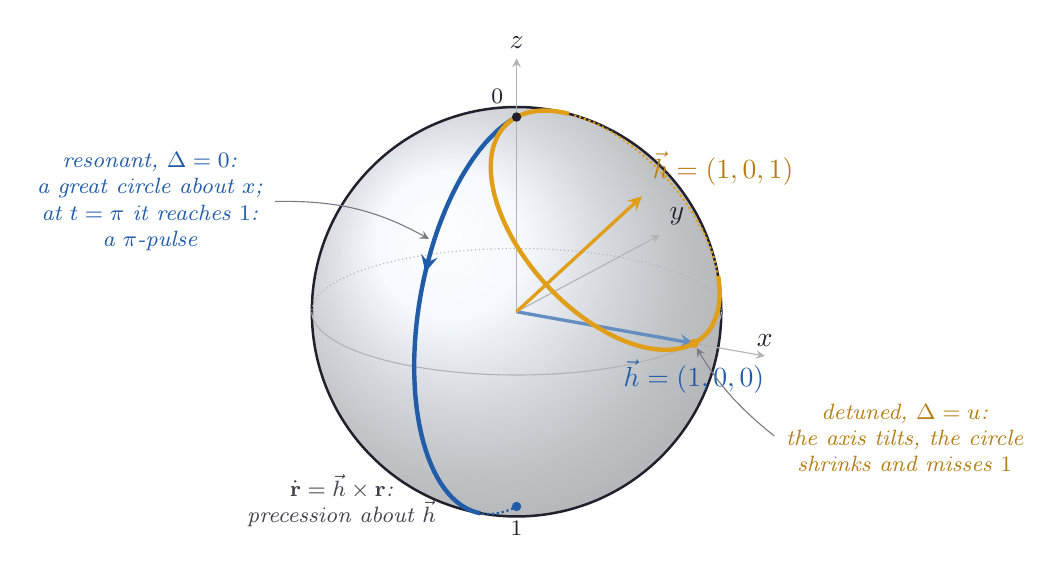
\begin{tikzpicture}[ink/.style={line width=0.9pt, ndInk}, faint/.style={line width=0.4pt, ndInk!35}, dashedink/.style={line width=0.5pt, ndInk!55, dash pattern=on 2.5pt off 2pt}, vec/.style={->, >=stealth, line width=1.2pt}, note/.style={font=\footnotesize\itshape, text=ndInk!85, align=center}, pointer/.style={->, >=stealth, line width=0.4pt, ndInk!60, shorten >=2pt, shorten <=1pt}, dot/.style={circle, fill=ndInk, inner sep=0pt, minimum size=3.4pt}, wash/.style={fill=ndSky, fill opacity=0.55}, every node/.style={text=ndInk}]
\definecolor{ndInk}{rgb}{0.13,0.13,0.18}
\definecolor{ndPaper}{rgb}{0.99,0.96,0.88}
\definecolor{ndSky}{rgb}{0.84,0.91,0.98}
\definecolor{ndRose}{rgb}{0.98,0.86,0.84}
\definecolor{ndBlue}{rgb}{0.13,0.36,0.66}
\definecolor{ndRed}{rgb}{0.78,0.20,0.16}
\definecolor{ndGold}{rgb}{0.88,0.62,0.10}
\definecolor{ndGreen}{rgb}{0.18,0.52,0.30}
\shade[ball color=ndSky!70!white, opacity=0.45] (0.000,0.000) circle (2.600);
\draw[ink] (0.000,0.000) circle (2.600);
\draw[faint] (-2.600,0.000) -- (-2.599,-0.021) -- (-2.596,-0.042) -- (-2.592,-0.063) -- (-2.586,-0.084) -- (-2.578,-0.105) -- (-2.568,-0.126) -- (-2.556,-0.146) -- (-2.543,-0.167) -- (-2.528,-0.188) -- (-2.511,-0.208) -- (-2.493,-0.228) -- (-2.473,-0.248) -- (-2.451,-0.268) -- (-2.427,-0.288) -- (-2.402,-0.307) -- (-2.375,-0.327) -- (-2.347,-0.346) -- (-2.317,-0.365) -- (-2.285,-0.383) -- (-2.252,-0.402) -- (-2.217,-0.420) -- (-2.181,-0.438) -- (-2.143,-0.455) -- (-2.103,-0.472) -- (-2.063,-0.489) -- (-2.021,-0.506) -- (-1.977,-0.522) -- (-1.932,-0.538) -- (-1.886,-0.553) -- (-1.838,-0.568) -- (-1.790,-0.583) -- (-1.740,-0.597) -- (-1.689,-0.611) -- (-1.636,-0.624) -- (-1.583,-0.637) -- (-1.528,-0.650) -- (-1.473,-0.662) -- (-1.416,-0.674) -- (-1.358,-0.685) -- (-1.300,-0.696) -- (-1.241,-0.706) -- (-1.180,-0.716) -- (-1.119,-0.725) -- (-1.058,-0.734) -- (-0.995,-0.742) -- (-0.932,-0.750) -- (-0.868,-0.757) -- (-0.803,-0.764) -- (-0.738,-0.770) -- (-0.673,-0.776) -- (-0.607,-0.781) -- (-0.541,-0.786) -- (-0.474,-0.790) -- (-0.407,-0.794) -- (-0.339,-0.797) -- (-0.272,-0.799) -- (-0.204,-0.801) -- (-0.136,-0.802) -- (-0.068,-0.803) -- (-0.000,-0.803) -- (0.068,-0.803) -- (0.136,-0.802) -- (0.204,-0.801) -- (0.272,-0.799) -- (0.339,-0.797) -- (0.407,-0.794) -- (0.474,-0.790) -- (0.541,-0.786) -- (0.607,-0.781) -- (0.673,-0.776) -- (0.738,-0.770) -- (0.803,-0.764) -- (0.868,-0.757) -- (0.932,-0.750) -- (0.995,-0.742) -- (1.058,-0.734) -- (1.119,-0.725) -- (1.180,-0.716) -- (1.241,-0.706) -- (1.300,-0.696) -- (1.358,-0.685) -- (1.416,-0.674) -- (1.473,-0.662) -- (1.528,-0.650) -- (1.583,-0.637) -- (1.636,-0.624) -- (1.689,-0.611) -- (1.740,-0.597) -- (1.790,-0.583) -- (1.838,-0.568) -- (1.886,-0.553) -- (1.932,-0.538) -- (1.977,-0.522) -- (2.021,-0.506) -- (2.063,-0.489) -- (2.103,-0.472) -- (2.143,-0.455) -- (2.181,-0.438) -- (2.217,-0.420) -- (2.252,-0.402) -- (2.285,-0.383) -- (2.317,-0.365) -- (2.347,-0.346) -- (2.375,-0.327) -- (2.402,-0.307) -- (2.427,-0.288) -- (2.451,-0.268) -- (2.473,-0.248) -- (2.493,-0.228) -- (2.511,-0.208) -- (2.528,-0.188) -- (2.543,-0.167) -- (2.556,-0.146) -- (2.568,-0.126) -- (2.578,-0.105) -- (2.586,-0.084) -- (2.592,-0.063) -- (2.596,-0.042) -- (2.599,-0.021) -- (2.600,-0.000);
\draw[faint, densely dotted] (1.300,0.696) -- (1.241,0.706) -- (1.180,0.716) -- (1.119,0.725) -- (1.058,0.734) -- (0.995,0.742) -- (0.932,0.750) -- (0.868,0.757) -- (0.803,0.764) -- (0.738,0.770) -- (0.673,0.776) -- (0.607,0.781) -- (0.541,0.786) -- (0.474,0.790) -- (0.407,0.794) -- (0.339,0.797) -- (0.272,0.799) -- (0.204,0.801) -- (0.136,0.802) -- (0.068,0.803) -- (0.000,0.803) -- (-0.068,0.803) -- (-0.136,0.802) -- (-0.204,0.801) -- (-0.272,0.799) -- (-0.339,0.797) -- (-0.407,0.794) -- (-0.474,0.790) -- (-0.541,0.786) -- (-0.607,0.781) -- (-0.673,0.776) -- (-0.738,0.770) -- (-0.803,0.764) -- (-0.868,0.757) -- (-0.932,0.750) -- (-0.995,0.742) -- (-1.058,0.734) -- (-1.119,0.725) -- (-1.180,0.716) -- (-1.241,0.706) -- (-1.300,0.696) -- (-1.358,0.685) -- (-1.416,0.674) -- (-1.473,0.662) -- (-1.528,0.650) -- (-1.583,0.637) -- (-1.636,0.624) -- (-1.689,0.611) -- (-1.740,0.597) -- (-1.790,0.583) -- (-1.838,0.568) -- (-1.886,0.553) -- (-1.932,0.538) -- (-1.977,0.522) -- (-2.021,0.506) -- (-2.063,0.489) -- (-2.103,0.472) -- (-2.143,0.455) -- (-2.181,0.438) -- (-2.217,0.420) -- (-2.252,0.402) -- (-2.285,0.383) -- (-2.317,0.365) -- (-2.347,0.346) -- (-2.375,0.327) -- (-2.402,0.307) -- (-2.427,0.288) -- (-2.451,0.268) -- (-2.473,0.248) -- (-2.493,0.228) -- (-2.511,0.208) -- (-2.528,0.188) -- (-2.543,0.167) -- (-2.556,0.146) -- (-2.568,0.126) -- (-2.578,0.105) -- (-2.586,0.084) -- (-2.592,0.063) -- (-2.596,0.042) -- (-2.599,0.021);
\draw[faint, densely dotted] (2.599,0.021) -- (2.596,0.042) -- (2.592,0.063) -- (2.586,0.084) -- (2.578,0.105) -- (2.568,0.126) -- (2.556,0.146) -- (2.543,0.167) -- (2.528,0.188) -- (2.511,0.208) -- (2.493,0.228) -- (2.473,0.248) -- (2.451,0.268) -- (2.427,0.288) -- (2.402,0.307) -- (2.375,0.327) -- (2.347,0.346) -- (2.317,0.365) -- (2.285,0.383) -- (2.252,0.402) -- (2.217,0.420) -- (2.181,0.438) -- (2.143,0.455) -- (2.103,0.472) -- (2.063,0.489) -- (2.021,0.506) -- (1.977,0.522) -- (1.932,0.538) -- (1.886,0.553) -- (1.838,0.568) -- (1.790,0.583) -- (1.740,0.597) -- (1.689,0.611) -- (1.636,0.624) -- (1.583,0.637) -- (1.528,0.650) -- (1.473,0.662) -- (1.416,0.674) -- (1.358,0.685) -- (1.300,0.696);
\draw[faint, ->, >=stealth] (0.000,0.000) -- (0.000,3.215) node[above] {$z$};
\draw[faint, ->, >=stealth] (0.000,0.000) -- (3.152,-0.562) node[above] {$x$};
\draw[faint, ->, >=stealth] (0.000,0.000) -- (1.820,0.974) node[above right] {$y$};
\draw[vec, ndBlue!70] (0.000,0.000) -- (2.252,-0.402) node[below, yshift=-2pt, text=ndBlue] {$\vec h=(1,0,0)$};
\draw[vec, ndGold] (0.000,0.000) -- (1.592,1.464) node[above right, text=ndGold!80!black] {$\vec h=(1,0,1)$};
\draw[line width=1.6pt, ndBlue] (0.000,2.473) -- (-0.020,2.462) -- (-0.041,2.450) -- (-0.061,2.437) -- (-0.082,2.424) -- (-0.102,2.411) -- (-0.122,2.396) -- (-0.143,2.381) -- (-0.163,2.366) -- (-0.183,2.350) -- (-0.203,2.333) -- (-0.224,2.316) -- (-0.244,2.299) -- (-0.264,2.280) -- (-0.284,2.261) -- (-0.303,2.242) -- (-0.323,2.222) -- (-0.343,2.202) -- (-0.363,2.180) -- (-0.382,2.159) -- (-0.402,2.137) -- (-0.421,2.114) -- (-0.440,2.091) -- (-0.460,2.067) -- (-0.479,2.043) -- (-0.497,2.018) -- (-0.516,1.993) -- (-0.535,1.967) -- (-0.554,1.941) -- (-0.572,1.914) -- (-0.590,1.887) -- (-0.608,1.860) -- (-0.626,1.832) -- (-0.644,1.803) -- (-0.662,1.774) -- (-0.679,1.745) -- (-0.697,1.715) -- (-0.714,1.685) -- (-0.731,1.654) -- (-0.748,1.623) -- (-0.764,1.592) -- (-0.781,1.560) -- (-0.797,1.527) -- (-0.813,1.495) -- (-0.829,1.462) -- (-0.844,1.428) -- (-0.860,1.395) -- (-0.875,1.361) -- (-0.890,1.326) -- (-0.905,1.292) -- (-0.919,1.256) -- (-0.934,1.221) -- (-0.948,1.185) -- (-0.962,1.150) -- (-0.975,1.113) -- (-0.989,1.077) -- (-1.002,1.040) -- (-1.015,1.003) -- (-1.027,0.966) -- (-1.040,0.928) -- (-1.052,0.891) -- (-1.064,0.853) -- (-1.075,0.814) -- (-1.087,0.776) -- (-1.098,0.737) -- (-1.108,0.699) -- (-1.119,0.660) -- (-1.129,0.621) -- (-1.139,0.582) -- (-1.149,0.542) -- (-1.158,0.503) -- (-1.167,0.463) -- (-1.176,0.423) -- (-1.185,0.383) -- (-1.193,0.343) -- (-1.201,0.303) -- (-1.209,0.263) -- (-1.216,0.223) -- (-1.223,0.183) -- (-1.230,0.143) -- (-1.236,0.102) -- (-1.243,0.062) -- (-1.248,0.022) -- (-1.254,-0.019) -- (-1.259,-0.059) -- (-1.264,-0.099) -- (-1.269,-0.140) -- (-1.273,-0.180) -- (-1.277,-0.220) -- (-1.281,-0.260) -- (-1.284,-0.300) -- (-1.287,-0.340) -- (-1.290,-0.380) -- (-1.292,-0.420) -- (-1.294,-0.460) -- (-1.296,-0.500) -- (-1.297,-0.539) -- (-1.299,-0.579) -- (-1.299,-0.618) -- (-1.300,-0.657) -- (-1.300,-0.696) -- (-1.300,-0.735) -- (-1.299,-0.773) -- (-1.299,-0.812) -- (-1.297,-0.850) -- (-1.296,-0.888) -- (-1.294,-0.925) -- (-1.292,-0.963) -- (-1.290,-1.000) -- (-1.287,-1.037) -- (-1.284,-1.074) -- (-1.281,-1.111) -- (-1.277,-1.147) -- (-1.273,-1.183) -- (-1.269,-1.218) -- (-1.264,-1.254) -- (-1.259,-1.289) -- (-1.254,-1.324) -- (-1.248,-1.358) -- (-1.243,-1.392) -- (-1.236,-1.426) -- (-1.230,-1.459) -- (-1.223,-1.492) -- (-1.216,-1.525) -- (-1.209,-1.557) -- (-1.201,-1.589) -- (-1.193,-1.621) -- (-1.185,-1.652) -- (-1.176,-1.682) -- (-1.167,-1.713) -- (-1.158,-1.743) -- (-1.149,-1.772) -- (-1.139,-1.801) -- (-1.129,-1.830) -- (-1.119,-1.858) -- (-1.108,-1.885) -- (-1.098,-1.912) -- (-1.087,-1.939) -- (-1.075,-1.965) -- (-1.064,-1.991) -- (-1.052,-2.016) -- (-1.040,-2.041) -- (-1.027,-2.065) -- (-1.015,-2.089) -- (-1.002,-2.112) -- (-0.989,-2.135) -- (-0.975,-2.157) -- (-0.962,-2.179) -- (-0.948,-2.200) -- (-0.934,-2.220) -- (-0.919,-2.241) -- (-0.905,-2.260) -- (-0.890,-2.279) -- (-0.875,-2.297) -- (-0.860,-2.315) -- (-0.844,-2.332) -- (-0.829,-2.349) -- (-0.813,-2.365) -- (-0.797,-2.380) -- (-0.781,-2.395) -- (-0.764,-2.409) -- (-0.748,-2.423) -- (-0.731,-2.436) -- (-0.714,-2.449) -- (-0.697,-2.461) -- (-0.679,-2.472) -- (-0.662,-2.483) -- (-0.644,-2.493) -- (-0.626,-2.502) -- (-0.608,-2.511) -- (-0.590,-2.519) -- (-0.572,-2.527) -- (-0.554,-2.534) -- (-0.535,-2.540) -- (-0.516,-2.546) -- (-0.497,-2.551) -- (-0.479,-2.555) -- (-0.460,-2.559);
\draw[line width=0.8pt, ndBlue, densely dotted] (-0.440,-2.562) -- (-0.421,-2.565) -- (-0.402,-2.567) -- (-0.382,-2.568) -- (-0.363,-2.569) -- (-0.343,-2.569) -- (-0.323,-2.568) -- (-0.303,-2.567) -- (-0.284,-2.565) -- (-0.264,-2.562) -- (-0.244,-2.559) -- (-0.224,-2.556) -- (-0.203,-2.551) -- (-0.183,-2.546) -- (-0.163,-2.540) -- (-0.143,-2.534) -- (-0.122,-2.527) -- (-0.102,-2.520) -- (-0.082,-2.512) -- (-0.061,-2.503) -- (-0.041,-2.493) -- (-0.020,-2.483) -- (-0.000,-2.473);
\draw[line width=1.6pt, ndGold] (0.000,2.473) -- (-0.028,2.457) -- (-0.055,2.439) -- (-0.082,2.420) -- (-0.106,2.400) -- (-0.130,2.378) -- (-0.152,2.355) -- (-0.173,2.331) -- (-0.193,2.305) -- (-0.212,2.278) -- (-0.229,2.250) -- (-0.245,2.221) -- (-0.259,2.191) -- (-0.272,2.159) -- (-0.284,2.126) -- (-0.295,2.093) -- (-0.304,2.058) -- (-0.311,2.022) -- (-0.317,1.985) -- (-0.322,1.948) -- (-0.325,1.909) -- (-0.327,1.870) -- (-0.328,1.829) -- (-0.327,1.788) -- (-0.324,1.746) -- (-0.320,1.704) -- (-0.315,1.661) -- (-0.308,1.617) -- (-0.300,1.573) -- (-0.291,1.528) -- (-0.280,1.482) -- (-0.267,1.436) -- (-0.254,1.390) -- (-0.238,1.344) -- (-0.222,1.297) -- (-0.204,1.250) -- (-0.185,1.202) -- (-0.165,1.155) -- (-0.143,1.107) -- (-0.120,1.059) -- (-0.096,1.012) -- (-0.071,0.964) -- (-0.045,0.916) -- (-0.017,0.869) -- (0.012,0.822) -- (0.042,0.774) -- (0.073,0.728) -- (0.105,0.681) -- (0.138,0.635) -- (0.172,0.589) -- (0.207,0.544) -- (0.242,0.499) -- (0.279,0.454) -- (0.317,0.410) -- (0.355,0.367) -- (0.394,0.325) -- (0.434,0.283) -- (0.474,0.242) -- (0.515,0.202) -- (0.557,0.162) -- (0.599,0.123) -- (0.642,0.086) -- (0.686,0.049) -- (0.729,0.013) -- (0.773,-0.022) -- (0.818,-0.055) -- (0.863,-0.088) -- (0.908,-0.120) -- (0.953,-0.150) -- (0.998,-0.179) -- (1.044,-0.207) -- (1.090,-0.234) -- (1.135,-0.260) -- (1.181,-0.284) -- (1.226,-0.307) -- (1.272,-0.329) -- (1.317,-0.349) -- (1.362,-0.368) -- (1.407,-0.386) -- (1.452,-0.402) -- (1.496,-0.416) -- (1.540,-0.430) -- (1.584,-0.442) -- (1.627,-0.452) -- (1.670,-0.461) -- (1.712,-0.468) -- (1.753,-0.474) -- (1.794,-0.479) -- (1.834,-0.482) -- (1.874,-0.483) -- (1.913,-0.483) -- (1.951,-0.482) -- (1.988,-0.479) -- (2.024,-0.474) -- (2.059,-0.468) -- (2.094,-0.461) -- (2.128,-0.452) -- (2.160,-0.442) -- (2.192,-0.430) -- (2.222,-0.416) -- (2.252,-0.402) -- (2.280,-0.386) -- (2.307,-0.368) -- (2.333,-0.349) -- (2.358,-0.329) -- (2.382,-0.307) -- (2.404,-0.284) -- (2.425,-0.260) -- (2.445,-0.234) -- (2.463,-0.207) -- (2.481,-0.179) -- (2.496,-0.150) -- (2.511,-0.120) -- (2.524,-0.088) -- (2.536,-0.055) -- (2.546,-0.022) -- (2.555,0.013) -- (2.563,0.049) -- (2.569,0.086) -- (2.574,0.123) -- (2.577,0.162) -- (2.579,0.201) -- (2.579,0.242) -- (2.578,0.283) -- (2.576,0.325) -- (2.572,0.367) -- (2.567,0.410) -- (2.560,0.454);
\draw[line width=1.6pt, ndGold] (0.668,2.513) -- (0.625,2.523) -- (0.582,2.532) -- (0.540,2.539) -- (0.499,2.545) -- (0.458,2.550) -- (0.417,2.553) -- (0.378,2.554) -- (0.339,2.554) -- (0.301,2.553) -- (0.264,2.550) -- (0.228,2.545) -- (0.192,2.539) -- (0.158,2.532) -- (0.124,2.523) -- (0.092,2.513) -- (0.060,2.501) -- (0.029,2.487) -- (-0.000,2.473);
\draw[line width=0.8pt, ndGold, densely dotted] (2.552,0.498) -- (2.542,0.543) -- (2.531,0.589) -- (2.519,0.635) -- (2.505,0.681) -- (2.490,0.727) -- (2.474,0.774) -- (2.456,0.821) -- (2.437,0.869) -- (2.417,0.916) -- (2.395,0.964) -- (2.372,1.012) -- (2.348,1.059) -- (2.323,1.107) -- (2.296,1.155) -- (2.269,1.202) -- (2.240,1.249) -- (2.210,1.297) -- (2.179,1.344) -- (2.147,1.390) -- (2.114,1.436) -- (2.080,1.482) -- (2.045,1.528) -- (2.009,1.572) -- (1.973,1.617) -- (1.935,1.661) -- (1.897,1.704) -- (1.858,1.746) -- (1.818,1.788) -- (1.777,1.829) -- (1.736,1.869) -- (1.694,1.909) -- (1.652,1.948) -- (1.609,1.985) -- (1.566,2.022) -- (1.522,2.058) -- (1.478,2.093) -- (1.434,2.126) -- (1.389,2.159) -- (1.344,2.191) -- (1.299,2.221) -- (1.253,2.250) -- (1.208,2.278) -- (1.162,2.305) -- (1.116,2.331) -- (1.071,2.355) -- (1.025,2.378) -- (0.980,2.400) -- (0.934,2.420) -- (0.889,2.439) -- (0.844,2.457) -- (0.800,2.473) -- (0.755,2.487) -- (0.711,2.501);
\draw[->, >=stealth, line width=1.6pt, ndBlue] (-1.129,0.621) -- (-1.158,0.503);
\node[dot, label={[font=\footnotesize]above left:$\ket0$}] at (0.000,2.473) {};
\node[dot, fill=ndBlue, label={[font=\footnotesize]below:$\ket1$}] at (0.000,-2.473) {};
\node[dot, fill=ndGold] at (2.252,-0.402) {};
\node[note, anchor=east, text=ndBlue] (a) at (-3.10,1.4) {resonant, $\Delta=0$:\\a great circle about $x$;\\ at $t=\pi$ it reaches $\ket1$:\\ a $\pi$-pulse};
\draw[pointer] (a.east) to[bend left=15] (-1.052,0.891);
\node[note, anchor=west, text=ndGold!80!black] (c) at (3.30,-1.6) {detuned, $\Delta=u$:\\the axis tilts, the circle\\ shrinks and misses $\ket1$};
\draw[pointer] (c.west) to[bend left=10] (2.252,-0.402);
\node[note, anchor=east] at (-0.90,-2.4) {$\dot{\mathbf r}=\vec h\times\mathbf r$:\\precession about $\vec h$};
\end{tikzpicture}

\caption{Bloch-sphere trajectories from $\ket0$ under $H=\tfrac\Delta2\sigz+\tfrac12\sigx$: resonant ($\Delta=0$, blue, a $\pi$-pulse reaching $\ket1$) and detuned ($\Delta=1$, gold). The arrows are the corresponding field vectors $\vec h$, the rotation axes. Generated by \texttt{code/ch02\_bloch.py}.}\label{fig:ch02:bloch}
\end{figure}}
\onp{\begin{center}\resizebox{!}{0.6\textheight}{% Generated by code/needham.py -- do not edit by hand.
\definecolor{qocA}{rgb}{0.00,0.45,0.70}
\definecolor{qocB}{rgb}{0.90,0.60,0.00}
\definecolor{qocC}{rgb}{0.00,0.62,0.45}
\definecolor{qocD}{rgb}{0.80,0.40,0.00}
\definecolor{qocE}{rgb}{0.80,0.60,0.70}
\definecolor{qocF}{rgb}{0.35,0.70,0.90}
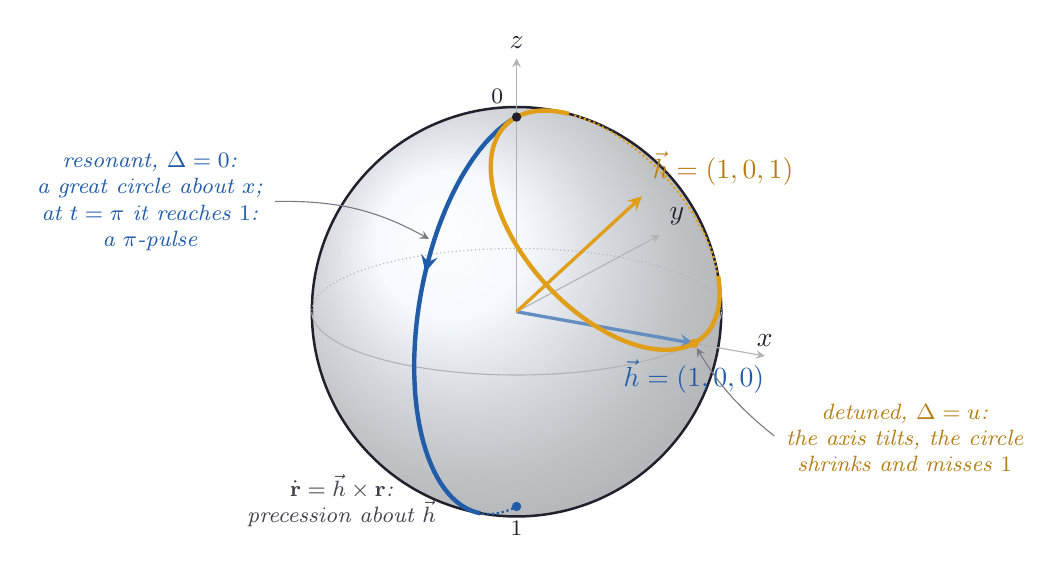
\begin{tikzpicture}[ink/.style={line width=0.9pt, ndInk}, faint/.style={line width=0.4pt, ndInk!35}, dashedink/.style={line width=0.5pt, ndInk!55, dash pattern=on 2.5pt off 2pt}, vec/.style={->, >=stealth, line width=1.2pt}, note/.style={font=\footnotesize\itshape, text=ndInk!85, align=center}, pointer/.style={->, >=stealth, line width=0.4pt, ndInk!60, shorten >=2pt, shorten <=1pt}, dot/.style={circle, fill=ndInk, inner sep=0pt, minimum size=3.4pt}, wash/.style={fill=ndSky, fill opacity=0.55}, every node/.style={text=ndInk}]
\definecolor{ndInk}{rgb}{0.13,0.13,0.18}
\definecolor{ndPaper}{rgb}{0.99,0.96,0.88}
\definecolor{ndSky}{rgb}{0.84,0.91,0.98}
\definecolor{ndRose}{rgb}{0.98,0.86,0.84}
\definecolor{ndBlue}{rgb}{0.13,0.36,0.66}
\definecolor{ndRed}{rgb}{0.78,0.20,0.16}
\definecolor{ndGold}{rgb}{0.88,0.62,0.10}
\definecolor{ndGreen}{rgb}{0.18,0.52,0.30}
\shade[ball color=ndSky!70!white, opacity=0.45] (0.000,0.000) circle (2.600);
\draw[ink] (0.000,0.000) circle (2.600);
\draw[faint] (-2.600,0.000) -- (-2.599,-0.021) -- (-2.596,-0.042) -- (-2.592,-0.063) -- (-2.586,-0.084) -- (-2.578,-0.105) -- (-2.568,-0.126) -- (-2.556,-0.146) -- (-2.543,-0.167) -- (-2.528,-0.188) -- (-2.511,-0.208) -- (-2.493,-0.228) -- (-2.473,-0.248) -- (-2.451,-0.268) -- (-2.427,-0.288) -- (-2.402,-0.307) -- (-2.375,-0.327) -- (-2.347,-0.346) -- (-2.317,-0.365) -- (-2.285,-0.383) -- (-2.252,-0.402) -- (-2.217,-0.420) -- (-2.181,-0.438) -- (-2.143,-0.455) -- (-2.103,-0.472) -- (-2.063,-0.489) -- (-2.021,-0.506) -- (-1.977,-0.522) -- (-1.932,-0.538) -- (-1.886,-0.553) -- (-1.838,-0.568) -- (-1.790,-0.583) -- (-1.740,-0.597) -- (-1.689,-0.611) -- (-1.636,-0.624) -- (-1.583,-0.637) -- (-1.528,-0.650) -- (-1.473,-0.662) -- (-1.416,-0.674) -- (-1.358,-0.685) -- (-1.300,-0.696) -- (-1.241,-0.706) -- (-1.180,-0.716) -- (-1.119,-0.725) -- (-1.058,-0.734) -- (-0.995,-0.742) -- (-0.932,-0.750) -- (-0.868,-0.757) -- (-0.803,-0.764) -- (-0.738,-0.770) -- (-0.673,-0.776) -- (-0.607,-0.781) -- (-0.541,-0.786) -- (-0.474,-0.790) -- (-0.407,-0.794) -- (-0.339,-0.797) -- (-0.272,-0.799) -- (-0.204,-0.801) -- (-0.136,-0.802) -- (-0.068,-0.803) -- (-0.000,-0.803) -- (0.068,-0.803) -- (0.136,-0.802) -- (0.204,-0.801) -- (0.272,-0.799) -- (0.339,-0.797) -- (0.407,-0.794) -- (0.474,-0.790) -- (0.541,-0.786) -- (0.607,-0.781) -- (0.673,-0.776) -- (0.738,-0.770) -- (0.803,-0.764) -- (0.868,-0.757) -- (0.932,-0.750) -- (0.995,-0.742) -- (1.058,-0.734) -- (1.119,-0.725) -- (1.180,-0.716) -- (1.241,-0.706) -- (1.300,-0.696) -- (1.358,-0.685) -- (1.416,-0.674) -- (1.473,-0.662) -- (1.528,-0.650) -- (1.583,-0.637) -- (1.636,-0.624) -- (1.689,-0.611) -- (1.740,-0.597) -- (1.790,-0.583) -- (1.838,-0.568) -- (1.886,-0.553) -- (1.932,-0.538) -- (1.977,-0.522) -- (2.021,-0.506) -- (2.063,-0.489) -- (2.103,-0.472) -- (2.143,-0.455) -- (2.181,-0.438) -- (2.217,-0.420) -- (2.252,-0.402) -- (2.285,-0.383) -- (2.317,-0.365) -- (2.347,-0.346) -- (2.375,-0.327) -- (2.402,-0.307) -- (2.427,-0.288) -- (2.451,-0.268) -- (2.473,-0.248) -- (2.493,-0.228) -- (2.511,-0.208) -- (2.528,-0.188) -- (2.543,-0.167) -- (2.556,-0.146) -- (2.568,-0.126) -- (2.578,-0.105) -- (2.586,-0.084) -- (2.592,-0.063) -- (2.596,-0.042) -- (2.599,-0.021) -- (2.600,-0.000);
\draw[faint, densely dotted] (1.300,0.696) -- (1.241,0.706) -- (1.180,0.716) -- (1.119,0.725) -- (1.058,0.734) -- (0.995,0.742) -- (0.932,0.750) -- (0.868,0.757) -- (0.803,0.764) -- (0.738,0.770) -- (0.673,0.776) -- (0.607,0.781) -- (0.541,0.786) -- (0.474,0.790) -- (0.407,0.794) -- (0.339,0.797) -- (0.272,0.799) -- (0.204,0.801) -- (0.136,0.802) -- (0.068,0.803) -- (0.000,0.803) -- (-0.068,0.803) -- (-0.136,0.802) -- (-0.204,0.801) -- (-0.272,0.799) -- (-0.339,0.797) -- (-0.407,0.794) -- (-0.474,0.790) -- (-0.541,0.786) -- (-0.607,0.781) -- (-0.673,0.776) -- (-0.738,0.770) -- (-0.803,0.764) -- (-0.868,0.757) -- (-0.932,0.750) -- (-0.995,0.742) -- (-1.058,0.734) -- (-1.119,0.725) -- (-1.180,0.716) -- (-1.241,0.706) -- (-1.300,0.696) -- (-1.358,0.685) -- (-1.416,0.674) -- (-1.473,0.662) -- (-1.528,0.650) -- (-1.583,0.637) -- (-1.636,0.624) -- (-1.689,0.611) -- (-1.740,0.597) -- (-1.790,0.583) -- (-1.838,0.568) -- (-1.886,0.553) -- (-1.932,0.538) -- (-1.977,0.522) -- (-2.021,0.506) -- (-2.063,0.489) -- (-2.103,0.472) -- (-2.143,0.455) -- (-2.181,0.438) -- (-2.217,0.420) -- (-2.252,0.402) -- (-2.285,0.383) -- (-2.317,0.365) -- (-2.347,0.346) -- (-2.375,0.327) -- (-2.402,0.307) -- (-2.427,0.288) -- (-2.451,0.268) -- (-2.473,0.248) -- (-2.493,0.228) -- (-2.511,0.208) -- (-2.528,0.188) -- (-2.543,0.167) -- (-2.556,0.146) -- (-2.568,0.126) -- (-2.578,0.105) -- (-2.586,0.084) -- (-2.592,0.063) -- (-2.596,0.042) -- (-2.599,0.021);
\draw[faint, densely dotted] (2.599,0.021) -- (2.596,0.042) -- (2.592,0.063) -- (2.586,0.084) -- (2.578,0.105) -- (2.568,0.126) -- (2.556,0.146) -- (2.543,0.167) -- (2.528,0.188) -- (2.511,0.208) -- (2.493,0.228) -- (2.473,0.248) -- (2.451,0.268) -- (2.427,0.288) -- (2.402,0.307) -- (2.375,0.327) -- (2.347,0.346) -- (2.317,0.365) -- (2.285,0.383) -- (2.252,0.402) -- (2.217,0.420) -- (2.181,0.438) -- (2.143,0.455) -- (2.103,0.472) -- (2.063,0.489) -- (2.021,0.506) -- (1.977,0.522) -- (1.932,0.538) -- (1.886,0.553) -- (1.838,0.568) -- (1.790,0.583) -- (1.740,0.597) -- (1.689,0.611) -- (1.636,0.624) -- (1.583,0.637) -- (1.528,0.650) -- (1.473,0.662) -- (1.416,0.674) -- (1.358,0.685) -- (1.300,0.696);
\draw[faint, ->, >=stealth] (0.000,0.000) -- (0.000,3.215) node[above] {$z$};
\draw[faint, ->, >=stealth] (0.000,0.000) -- (3.152,-0.562) node[above] {$x$};
\draw[faint, ->, >=stealth] (0.000,0.000) -- (1.820,0.974) node[above right] {$y$};
\draw[vec, ndBlue!70] (0.000,0.000) -- (2.252,-0.402) node[below, yshift=-2pt, text=ndBlue] {$\vec h=(1,0,0)$};
\draw[vec, ndGold] (0.000,0.000) -- (1.592,1.464) node[above right, text=ndGold!80!black] {$\vec h=(1,0,1)$};
\draw[line width=1.6pt, ndBlue] (0.000,2.473) -- (-0.020,2.462) -- (-0.041,2.450) -- (-0.061,2.437) -- (-0.082,2.424) -- (-0.102,2.411) -- (-0.122,2.396) -- (-0.143,2.381) -- (-0.163,2.366) -- (-0.183,2.350) -- (-0.203,2.333) -- (-0.224,2.316) -- (-0.244,2.299) -- (-0.264,2.280) -- (-0.284,2.261) -- (-0.303,2.242) -- (-0.323,2.222) -- (-0.343,2.202) -- (-0.363,2.180) -- (-0.382,2.159) -- (-0.402,2.137) -- (-0.421,2.114) -- (-0.440,2.091) -- (-0.460,2.067) -- (-0.479,2.043) -- (-0.497,2.018) -- (-0.516,1.993) -- (-0.535,1.967) -- (-0.554,1.941) -- (-0.572,1.914) -- (-0.590,1.887) -- (-0.608,1.860) -- (-0.626,1.832) -- (-0.644,1.803) -- (-0.662,1.774) -- (-0.679,1.745) -- (-0.697,1.715) -- (-0.714,1.685) -- (-0.731,1.654) -- (-0.748,1.623) -- (-0.764,1.592) -- (-0.781,1.560) -- (-0.797,1.527) -- (-0.813,1.495) -- (-0.829,1.462) -- (-0.844,1.428) -- (-0.860,1.395) -- (-0.875,1.361) -- (-0.890,1.326) -- (-0.905,1.292) -- (-0.919,1.256) -- (-0.934,1.221) -- (-0.948,1.185) -- (-0.962,1.150) -- (-0.975,1.113) -- (-0.989,1.077) -- (-1.002,1.040) -- (-1.015,1.003) -- (-1.027,0.966) -- (-1.040,0.928) -- (-1.052,0.891) -- (-1.064,0.853) -- (-1.075,0.814) -- (-1.087,0.776) -- (-1.098,0.737) -- (-1.108,0.699) -- (-1.119,0.660) -- (-1.129,0.621) -- (-1.139,0.582) -- (-1.149,0.542) -- (-1.158,0.503) -- (-1.167,0.463) -- (-1.176,0.423) -- (-1.185,0.383) -- (-1.193,0.343) -- (-1.201,0.303) -- (-1.209,0.263) -- (-1.216,0.223) -- (-1.223,0.183) -- (-1.230,0.143) -- (-1.236,0.102) -- (-1.243,0.062) -- (-1.248,0.022) -- (-1.254,-0.019) -- (-1.259,-0.059) -- (-1.264,-0.099) -- (-1.269,-0.140) -- (-1.273,-0.180) -- (-1.277,-0.220) -- (-1.281,-0.260) -- (-1.284,-0.300) -- (-1.287,-0.340) -- (-1.290,-0.380) -- (-1.292,-0.420) -- (-1.294,-0.460) -- (-1.296,-0.500) -- (-1.297,-0.539) -- (-1.299,-0.579) -- (-1.299,-0.618) -- (-1.300,-0.657) -- (-1.300,-0.696) -- (-1.300,-0.735) -- (-1.299,-0.773) -- (-1.299,-0.812) -- (-1.297,-0.850) -- (-1.296,-0.888) -- (-1.294,-0.925) -- (-1.292,-0.963) -- (-1.290,-1.000) -- (-1.287,-1.037) -- (-1.284,-1.074) -- (-1.281,-1.111) -- (-1.277,-1.147) -- (-1.273,-1.183) -- (-1.269,-1.218) -- (-1.264,-1.254) -- (-1.259,-1.289) -- (-1.254,-1.324) -- (-1.248,-1.358) -- (-1.243,-1.392) -- (-1.236,-1.426) -- (-1.230,-1.459) -- (-1.223,-1.492) -- (-1.216,-1.525) -- (-1.209,-1.557) -- (-1.201,-1.589) -- (-1.193,-1.621) -- (-1.185,-1.652) -- (-1.176,-1.682) -- (-1.167,-1.713) -- (-1.158,-1.743) -- (-1.149,-1.772) -- (-1.139,-1.801) -- (-1.129,-1.830) -- (-1.119,-1.858) -- (-1.108,-1.885) -- (-1.098,-1.912) -- (-1.087,-1.939) -- (-1.075,-1.965) -- (-1.064,-1.991) -- (-1.052,-2.016) -- (-1.040,-2.041) -- (-1.027,-2.065) -- (-1.015,-2.089) -- (-1.002,-2.112) -- (-0.989,-2.135) -- (-0.975,-2.157) -- (-0.962,-2.179) -- (-0.948,-2.200) -- (-0.934,-2.220) -- (-0.919,-2.241) -- (-0.905,-2.260) -- (-0.890,-2.279) -- (-0.875,-2.297) -- (-0.860,-2.315) -- (-0.844,-2.332) -- (-0.829,-2.349) -- (-0.813,-2.365) -- (-0.797,-2.380) -- (-0.781,-2.395) -- (-0.764,-2.409) -- (-0.748,-2.423) -- (-0.731,-2.436) -- (-0.714,-2.449) -- (-0.697,-2.461) -- (-0.679,-2.472) -- (-0.662,-2.483) -- (-0.644,-2.493) -- (-0.626,-2.502) -- (-0.608,-2.511) -- (-0.590,-2.519) -- (-0.572,-2.527) -- (-0.554,-2.534) -- (-0.535,-2.540) -- (-0.516,-2.546) -- (-0.497,-2.551) -- (-0.479,-2.555) -- (-0.460,-2.559);
\draw[line width=0.8pt, ndBlue, densely dotted] (-0.440,-2.562) -- (-0.421,-2.565) -- (-0.402,-2.567) -- (-0.382,-2.568) -- (-0.363,-2.569) -- (-0.343,-2.569) -- (-0.323,-2.568) -- (-0.303,-2.567) -- (-0.284,-2.565) -- (-0.264,-2.562) -- (-0.244,-2.559) -- (-0.224,-2.556) -- (-0.203,-2.551) -- (-0.183,-2.546) -- (-0.163,-2.540) -- (-0.143,-2.534) -- (-0.122,-2.527) -- (-0.102,-2.520) -- (-0.082,-2.512) -- (-0.061,-2.503) -- (-0.041,-2.493) -- (-0.020,-2.483) -- (-0.000,-2.473);
\draw[line width=1.6pt, ndGold] (0.000,2.473) -- (-0.028,2.457) -- (-0.055,2.439) -- (-0.082,2.420) -- (-0.106,2.400) -- (-0.130,2.378) -- (-0.152,2.355) -- (-0.173,2.331) -- (-0.193,2.305) -- (-0.212,2.278) -- (-0.229,2.250) -- (-0.245,2.221) -- (-0.259,2.191) -- (-0.272,2.159) -- (-0.284,2.126) -- (-0.295,2.093) -- (-0.304,2.058) -- (-0.311,2.022) -- (-0.317,1.985) -- (-0.322,1.948) -- (-0.325,1.909) -- (-0.327,1.870) -- (-0.328,1.829) -- (-0.327,1.788) -- (-0.324,1.746) -- (-0.320,1.704) -- (-0.315,1.661) -- (-0.308,1.617) -- (-0.300,1.573) -- (-0.291,1.528) -- (-0.280,1.482) -- (-0.267,1.436) -- (-0.254,1.390) -- (-0.238,1.344) -- (-0.222,1.297) -- (-0.204,1.250) -- (-0.185,1.202) -- (-0.165,1.155) -- (-0.143,1.107) -- (-0.120,1.059) -- (-0.096,1.012) -- (-0.071,0.964) -- (-0.045,0.916) -- (-0.017,0.869) -- (0.012,0.822) -- (0.042,0.774) -- (0.073,0.728) -- (0.105,0.681) -- (0.138,0.635) -- (0.172,0.589) -- (0.207,0.544) -- (0.242,0.499) -- (0.279,0.454) -- (0.317,0.410) -- (0.355,0.367) -- (0.394,0.325) -- (0.434,0.283) -- (0.474,0.242) -- (0.515,0.202) -- (0.557,0.162) -- (0.599,0.123) -- (0.642,0.086) -- (0.686,0.049) -- (0.729,0.013) -- (0.773,-0.022) -- (0.818,-0.055) -- (0.863,-0.088) -- (0.908,-0.120) -- (0.953,-0.150) -- (0.998,-0.179) -- (1.044,-0.207) -- (1.090,-0.234) -- (1.135,-0.260) -- (1.181,-0.284) -- (1.226,-0.307) -- (1.272,-0.329) -- (1.317,-0.349) -- (1.362,-0.368) -- (1.407,-0.386) -- (1.452,-0.402) -- (1.496,-0.416) -- (1.540,-0.430) -- (1.584,-0.442) -- (1.627,-0.452) -- (1.670,-0.461) -- (1.712,-0.468) -- (1.753,-0.474) -- (1.794,-0.479) -- (1.834,-0.482) -- (1.874,-0.483) -- (1.913,-0.483) -- (1.951,-0.482) -- (1.988,-0.479) -- (2.024,-0.474) -- (2.059,-0.468) -- (2.094,-0.461) -- (2.128,-0.452) -- (2.160,-0.442) -- (2.192,-0.430) -- (2.222,-0.416) -- (2.252,-0.402) -- (2.280,-0.386) -- (2.307,-0.368) -- (2.333,-0.349) -- (2.358,-0.329) -- (2.382,-0.307) -- (2.404,-0.284) -- (2.425,-0.260) -- (2.445,-0.234) -- (2.463,-0.207) -- (2.481,-0.179) -- (2.496,-0.150) -- (2.511,-0.120) -- (2.524,-0.088) -- (2.536,-0.055) -- (2.546,-0.022) -- (2.555,0.013) -- (2.563,0.049) -- (2.569,0.086) -- (2.574,0.123) -- (2.577,0.162) -- (2.579,0.201) -- (2.579,0.242) -- (2.578,0.283) -- (2.576,0.325) -- (2.572,0.367) -- (2.567,0.410) -- (2.560,0.454);
\draw[line width=1.6pt, ndGold] (0.668,2.513) -- (0.625,2.523) -- (0.582,2.532) -- (0.540,2.539) -- (0.499,2.545) -- (0.458,2.550) -- (0.417,2.553) -- (0.378,2.554) -- (0.339,2.554) -- (0.301,2.553) -- (0.264,2.550) -- (0.228,2.545) -- (0.192,2.539) -- (0.158,2.532) -- (0.124,2.523) -- (0.092,2.513) -- (0.060,2.501) -- (0.029,2.487) -- (-0.000,2.473);
\draw[line width=0.8pt, ndGold, densely dotted] (2.552,0.498) -- (2.542,0.543) -- (2.531,0.589) -- (2.519,0.635) -- (2.505,0.681) -- (2.490,0.727) -- (2.474,0.774) -- (2.456,0.821) -- (2.437,0.869) -- (2.417,0.916) -- (2.395,0.964) -- (2.372,1.012) -- (2.348,1.059) -- (2.323,1.107) -- (2.296,1.155) -- (2.269,1.202) -- (2.240,1.249) -- (2.210,1.297) -- (2.179,1.344) -- (2.147,1.390) -- (2.114,1.436) -- (2.080,1.482) -- (2.045,1.528) -- (2.009,1.572) -- (1.973,1.617) -- (1.935,1.661) -- (1.897,1.704) -- (1.858,1.746) -- (1.818,1.788) -- (1.777,1.829) -- (1.736,1.869) -- (1.694,1.909) -- (1.652,1.948) -- (1.609,1.985) -- (1.566,2.022) -- (1.522,2.058) -- (1.478,2.093) -- (1.434,2.126) -- (1.389,2.159) -- (1.344,2.191) -- (1.299,2.221) -- (1.253,2.250) -- (1.208,2.278) -- (1.162,2.305) -- (1.116,2.331) -- (1.071,2.355) -- (1.025,2.378) -- (0.980,2.400) -- (0.934,2.420) -- (0.889,2.439) -- (0.844,2.457) -- (0.800,2.473) -- (0.755,2.487) -- (0.711,2.501);
\draw[->, >=stealth, line width=1.6pt, ndBlue] (-1.129,0.621) -- (-1.158,0.503);
\node[dot, label={[font=\footnotesize]above left:$\ket0$}] at (0.000,2.473) {};
\node[dot, fill=ndBlue, label={[font=\footnotesize]below:$\ket1$}] at (0.000,-2.473) {};
\node[dot, fill=ndGold] at (2.252,-0.402) {};
\node[note, anchor=east, text=ndBlue] (a) at (-3.10,1.4) {resonant, $\Delta=0$:\\a great circle about $x$;\\ at $t=\pi$ it reaches $\ket1$:\\ a $\pi$-pulse};
\draw[pointer] (a.east) to[bend left=15] (-1.052,0.891);
\node[note, anchor=west, text=ndGold!80!black] (c) at (3.30,-1.6) {detuned, $\Delta=u$:\\the axis tilts, the circle\\ shrinks and misses $\ket1$};
\draw[pointer] (c.west) to[bend left=10] (2.252,-0.402);
\node[note, anchor=east] at (-0.90,-2.4) {$\dot{\mathbf r}=\vec h\times\mathbf r$:\\precession about $\vec h$};
\end{tikzpicture}
}\end{center}}
\end{frame}

\section{Generalised measurements}\label{sec:ch02:povm}

\begin{frame}\ft{POVMs}
\begin{defn}[POVM]\label{def:ch02:povm}
A positive operator-valued measure on $\Hil$ with outcome set $\{1,\dots,m\}$ is a family $E_1,\dots,E_m\succeq 0$ with $\sum_j E_j=\Id$. Outcome $j$ occurs with probability $\Tr(E_j\rho)$.
\end{defn}
\ona{POVMs describe projective measurements on a larger system followed by discarding the ancilla, and are the correct model for the readout of real devices.}
\begin{exm}[Noisy qubit readout]\label{exm:ch02:noisy-readout}
A qubit readout reports ``0'' for a system in $\ket1$ with probability $\epsilon_1$, and ``1'' for a system in $\ket0$ with probability $\epsilon_0$. Its POVM is
\[
E_0=(1-\epsilon_0)\ket0\bra0+\epsilon_1\ket1\bra1,\qquad
E_1=\epsilon_0\ket0\bra0+(1-\epsilon_1)\ket1\bra1 .
\]
Both are $\succeq0$ and $E_0+E_1=\Id$. For $\epsilon_0,\epsilon_1>0$ neither is a projector.
\end{exm}
\ona{Only the diagonal of $\rho$ enters $\Tr(E_j\rho)$: we have $\Prob(0)=(1-\epsilon_0)\rho_{00}+\epsilon_1\rho_{11}$, the \emph{assignment} or \emph{confusion} matrix of the device acting on the populations. Typical values on superconducting qubits are $\epsilon_0,\epsilon_1$ of about $1$--$5\%$, with $\epsilon_1>\epsilon_0$ because $\ket1$ may decay during the readout. A POVM is \emph{informationally complete} if the map $\rho\mapsto(\Tr(E_j\rho))_j$ is injective on density operators; this is the static version of observability, cf.\ \Chap~\ref{C.StateSpace}. Informational completeness has a clean linear-algebra characterisation: the POVM is informationally complete if and only if the $E_j$ span the real vector space $\Herm[\Hil]$ of Hermitian matrices, which has dimension $N^2$. In particular it needs at least $N^2$ outcomes. For the proof, note that $\sum_jE_j=\Id$ always lies in the span. If the span is not all of $\Herm[\Hil]$, some non-zero Hermitian $X$ is orthogonal to it, $\Tr(E_jX)=0$ for all $j$; then $X$ is traceless (being orthogonal to $\Id$), and $\tfrac1N\Id\pm\epsilon X$ are two different density operators, for small $\epsilon>0$, that produce identical statistics. Conversely, if the $E_j$ span $\Herm[\Hil]$, the numbers $\Tr(E_j\rho)$ determine $\Tr(A\rho)$ for every Hermitian $A$, and hence $\rho$. The readout above is not informationally complete, since it cannot distinguish $\ket+$ from $\ket-$: its two elements span only the diagonal matrices. The four-outcome \emph{tetrahedral} POVM $E_j=\tfrac14(\Id+\vec n_j\cdot\vec\sigma)$ is informationally complete, where $\vec n_1,\dots,\vec n_4$ are the vertices of a regular tetrahedron inscribed in the Bloch sphere; $\sum_j\vec n_j=0$ gives $\sum_jE_j=\Id$. It has more outcomes than the dimension $N=2$, which no projective measurement can have, and it is minimal, since $4=N^2$.}
\onp{Informationally complete $\Leftrightarrow$ $\rho\mapsto(\Tr(E_j\rho))_j$ injective $\Leftrightarrow$ the $E_j$ span $\Herm[\Hil]$: needs $\ge N^2$ outcomes. The example is not: blind to $\ket\pm$.}
\end{frame}

\section{The coherence vector in the $\liesu[N]$ basis}

\begin{frame}\ft{An orthonormal basis of Hermitian matrices}
\ona{The Bloch construction generalises to any $N$, and the generalisation is the state-space representation on which the identifiability theory of \Chaps~\ref{C.Open}--\ref{C.Frequency} is built. We consider Hermitian traceless Hamiltonians. This is a reasonable setup since the nonzero trace part leaves the dynamics unchanged up to a global phase, and removing it fixes the ambiguity in the generator. Such Hamiltonians lie in the real vector space of traceless Hermitian $N\times N$ matrices, of dimension $n\coloneqq N^{2}-1$. We introduce a complete set of basis operators,}
\onp{Generalise the Bloch vector to $N$ levels. Basis of Hermitian matrices:}
\begin{equation}\label{eq:ch02:basis_conditions}
    \{F_j\}_{j=0}^{N^2-1},\quad F_0=\tfrac{1}{\sqrt{N}}\Id,\quad F_j=F_j^\dagger,\quad \Tr(F_jF_k)=\delta_{jk},
\end{equation}
\ona{so that the $F_j$ for $j\geq1$ are traceless: $\mathcal F=\{F_{j}\}_{j=1}^{n}$ is an orthonormal basis of traceless Hermitian matrices, equivalently a basis of $\liesu[N]$ up to an overall factor of $\imath$. For $N=2^q$ the natural choice is the (normalised) Pauli strings. Every traceless Hamiltonian admits the unique expansion}
\onp{For $N=2^q$: normalised Pauli strings. Unique expansions}
\begin{equation}\label{eq:ch02:decomposition_hamiltonian}
    H = \sum_{j=1}^{n}\theta_{j}F_{j},
    \qquad \theta_{j}=\Tr[F_{j}H]\in\R,
\end{equation}
\ona{and we collect the coefficients in $\vec{\theta}=[\theta_{1},\dots,\theta_{n}]^{\top}\in\R^{n}$, which is the vector to be identified in \Chap~\ref{C.StateSpace}. Due to physical constraints of the system, only a small number $P$ of these coefficients is nonzero in practice, typically $P \ll n$ \cite{Zhang2014}. The density operator can also be decomposed in terms of these generators,}
\begin{equation}\label{eq:ch02:coherence}
    \rho = \tfrac{1}{N}\Id +  \sum_{j=1}^{n} x_{j}F_{j},\qquad x_{j} \coloneqq \Tr[F_{j}\rho].
\end{equation}
\ona{Here $\rho$ is parameterised by $n$ elements $x_{j}$ of the \emph{coherence vector} $\vec{x}$. Since each $F_{j}$ is an observable, these elements are simply their expectation values, which can be obtained by measurements: the state is encoded in the set of expectation values of a complete set of independent observables $\{F_{j}\}$.}
\onp{$\vec\theta$: parameters to identify (\Chap~\ref{C.StateSpace}); $\vec x$: \alert{coherence vector} of expectation values.}
\end{frame}

\begin{frame}\ft{The shape of the state space}
\ona{For a qubit, the coherence vector (a multiple of the Bloch vector) fills a ball. For $N>2$ this is no longer true, and the reader should not carry the Bloch-ball picture over. The set $\Dens[\C^N]$ of density operators is a compact convex set of real dimension $n=N^2-1$. Its \emph{extreme points}, the states that are not mixtures of other states, are exactly the pure states $\ket\psi\bra\psi$. These form the complex projective space $\C P^{N-1}$ (unit vectors up to phase), a manifold of real dimension $2N-2$. For $N=2$ this is the whole boundary sphere $S^2$ of the Bloch ball. For $N>2$ it is a thin subset of the boundary, which has dimension $N^2-2>2N-2$; the rest of the boundary consists of mixed states of lower rank.}
\onp{\begin{itemize}\setlength\itemsep{0.4em}
    \item $\Dens[\C^N]$: compact convex, dimension $N^2-1$; extreme points $=$ pure states $\cong\C P^{N-1}$, dimension $2N-2$.
    \item $N=2$: the pure states are the whole boundary sphere. $N>2$: only a thin part of the boundary.
\end{itemize}}
\ona{In coherence-vector coordinates \eqref{eq:ch02:coherence}, $\Tr\rho^2=\tfrac1N+\norm{\vec x}^2\le1$, so every state satisfies}
\onp{Coherence vectors lie between two balls:}
\begin{equation}\label{eq:ch02:balls}
\norm{\vec x}\le\sqrt{1-\tfrac1N},\qquad\text{and every } \vec x \text{ with } \norm{\vec x}\le\tfrac1{\sqrt{N(N-1)}} \text{ is a state.}
\end{equation}
\ona{Equality in the first bound holds exactly for pure states. The bound is necessary but, for $N>2$, not sufficient. Take $N=3$ and the traceless direction $F=\operatorname{diag}(1,1,-2)/\sqrt6$. Then $\rho=\tfrac13\Id+cF$ has eigenvalues $\tfrac13+\tfrac{c}{\sqrt6}$ (twice) and $\tfrac13-\tfrac{2c}{\sqrt6}$. It is a state for $-\sqrt{2/3}\le c\le 1/\sqrt6$ only: at $c=-\sqrt{2/3}$ it is the pure state $\ket2\bra2$, on the outer sphere, but already at $c=0.8<\sqrt{2/3}$ it has a negative eigenvalue. The state space thus touches the outer sphere of \eqref{eq:ch02:balls} at the pure states and the inner sphere in other directions. It lies strictly between the two balls, and it is not symmetric under $\vec x\mapsto-\vec x$. The second statement of \eqref{eq:ch02:balls} holds because the eigenvalues of the traceless matrix $X=\rho-\tfrac1N\Id$ satisfy $\lambda_{\min}(X)\ge-\norm X\sqrt{(N-1)/N}$, which is $\ge-\tfrac1N$ when $\norm X\le1/\sqrt{N(N-1)}$.}
\onp{The outer bound is necessary, not sufficient: for $N=3$, $\tfrac13\Id+0.8\operatorname{diag}(1,1,-2)/\sqrt6$ has a negative eigenvalue. Not symmetric under $\vec x\mapsto-\vec x$.}
\end{frame}

\begin{frame}\ft{Structure constants}
\ona{The anti-symmetric and symmetric structure constants, $f_{jkl}$ and $g_{jkl}$ respectively, are defined through the commutation and anti-commutation relations}
\onp{Products of basis elements are encoded by \alert{structure constants}:}
\begin{align}\label{eq:ch02:antisymmetric_structure_const}
        \comm{F_{j}}{F_{k}} &= \imath\sum_{l=1}^{n} f_{jkl}F_{l}, \\ \label{eq:ch02:symmetric_structure_const}
        \acomm{F_{j}}{F_{k}} &= \tfrac{2}{N}\delta_{jk}\Id + \sum_{l=1}^{n} g_{jkl}F_{l}.
\end{align}
\ona{Adding the two, $F_jF_k=\tfrac1N\delta_{jk}\Id+\tfrac{\imath}{2}\sum_l\bar z_{jkl}F_l$ with $z_{jkl}=f_{jkl}+\imath g_{jkl}$. For $\liesu[2]$ the basis \eqref{eq:ch02:basis_conditions} is $F_j=\sigma_j/\sqrt2$, and \eqref{eq:ch02:pauli-comm} gives $f_{jkl}=\sqrt2\,\varepsilon_{jkl}$ and $g_{jkl}=0$. (The unnormalised Pauli matrices satisfy $\comm{\sigma_j}{\sigma_k}=2\imath\sum_l\varepsilon_{jkl}\sigma_l$, i.e.\ ``$f=2\varepsilon$'', but they violate $\Tr(F_jF_k)=\delta_{jk}$, and \eqref{eq:ch02:symmetric_structure_const} does not hold for them.) The rescaling $F_j\to cF_j$ sends $f\to cf$ and $g\to cg$, and therefore neither creates nor destroys non-zero structure constants.}
\end{frame}

\begin{frame}\ft{The Liouville--von Neumann equation in coherence-vector form}
\begin{propn}[Liouville--von Neumann in coherence-vector form]\label{prop:ch02:lvn-coherence}
For $H=\sum_k\theta_kF_k$, the components of the coherence vector obey the real linear system
$\dot x_i=\sum_{j,k}\theta_kf_{kji}\,x_j$, i.e.\ $\dot{\vec x}=\Amat^{(l)}\vec x$ with $\Amat^{(l)}_{ij}=-\sum_k\theta_kf_{ijk}$, an antisymmetric matrix. Under a control-affine Hamiltonian \eqref{eq:control-hamiltonian} with $\Hctrl=F_k$ one obtains the bilinear system $\dot{\vec x}=\big(\Amat^{(l)}+\sum_k u_k\Nmat_k\big)\vec x$ with $(\Nmat_k)_{ij}=-f_{kij}$.
\end{propn}
\ona{The superscript in $\Amat^{(l)}$ stands for the Liouville--von Neumann (unitary) part; in \Chap~\ref{C.Open} a dissipative part $\Amat^{(d)}$ is added. For the qubit, $H=\tfrac12\vec h\cdot\vec\sigma$ gives $\theta_k=h_k/\sqrt2$ and $x_j=r_j/\sqrt2$, and the proposition becomes $\dot r_i=\sum_{j,k}\varepsilon_{ikj}h_kr_j=(\vec h\times\Bloch)_i$, which is \eqref{eq:ch02:bloch-cross}.}
\ona{\begin{pf}
$\dot x_i=\Tr[F_i\dot\rho]=-\imath\sum_k\theta_k\Tr[F_i\comm{F_k}{\rho}]=-\imath\sum_k\theta_k\Tr[\comm{F_i}{F_k}\rho]=\sum_{j,k}\theta_kf_{ikj}\Tr[F_j\rho]$, using $\Tr[A\comm{B}{C}]=\Tr[\comm{A}{B}C]$ and \eqref{eq:ch02:antisymmetric_structure_const}; then $f_{ikj}=f_{kji}$ by total antisymmetry. The control term is identical with $\theta_k$ replaced by $u_k$. Antisymmetry of $\Amat^{(l)}$ reflects $\dd{t}\norm{\vec x}^2=0$, i.e.\ conservation of purity $\Tr\rho^2=\tfrac1N+\norm{\vec x}^2$.
\end{pf}}
\onp{For $\liesu[2]$, $F_j=\sigma_j/\sqrt2$: $f_{jkl}=\sqrt2\,\varepsilon_{jkl}$, $g=0$, and the proposition is the Bloch equation \eqref{eq:ch02:bloch}. $\Amat^{(l)}$ antisymmetric $\Leftrightarrow$ purity $\Tr\rho^2=\tfrac1N+\norm{\vec x}^2$ conserved.}
\end{frame}

\begin{frame}\ft{Structure constants of $\liesu[2^q]$ in the Pauli basis}
\begin{propn}\label{prop:ch02:su2q}
Let $F_j=P_j/\sqrt{2^q}$, where $P_1,\dots,P_n$ are the non-identity Pauli strings on $q$ qubits. For $j\ne k$ there is exactly one index $l$ with $P_jP_k\propto P_l$, and exactly one of the two families $(f_{jkl'})_{l'}$ and $(g_{jkl'})_{l'}$ is non-zero; it is non-zero only at $l'=l$. Moreover $g_{jjl}=0$ for all $j,l$.
\end{propn}
\ona{\begin{pf}
For single qubits, $\sigma_a\sigma_b\in\{\pm1,\pm\imath\}\cdot\sigma_c$ for some $c\in\{0,x,y,z\}$, with $\sigma_0=\Id$, by \eqref{eq:ch02:pauli-comm}. Taking tensor products factor by factor, $P_jP_k=c\,P_l$ with $c\in\{\pm1,\pm\imath\}$ and a single string $P_l$, which is not the identity string unless $P_j=P_k$. Since the $P$'s are Hermitian, $P_kP_j=(P_jP_k)^\dagger=\bar c\,P_l$. If $c$ is real, $P_j$ and $P_k$ commute, so $\comm{P_j}{P_k}=0$ and $\acomm{P_j}{P_k}=2c\,P_l$. If $c$ is imaginary, they anticommute, so $\acomm{P_j}{P_k}=0$ and $\comm{P_j}{P_k}=2c\,P_l$. Either way exactly one of the two is non-zero, and it is a multiple of the single basis element $F_l$. Finally, $P_j^2=\Id$, so $\acomm{F_j}{F_j}=\tfrac2{2^q}\Id$ has no component along any $F_l$ with $l\ge1$. The normalisation only rescales $f$ and $g$ by a common constant.
\end{pf}}
\ona{The property is basis dependent: for $\liesu[3]$ in the Gell-Mann basis, the pair $(4,5)$ has two non-zero structure constants, $f_{453}=\tfrac12$ and $f_{458}=\tfrac{\sqrt3}{2}$. Its consequence for the coherence-vector equations is extreme sparsity. Each entry $\Amat^{(l)}_{ij}=-\sum_k\theta_kf_{ijk}$ involves a single parameter $\theta_k$, namely the one with $P_iP_j\propto P_k$, and each row of each $\Nmat_k$ has at most one non-zero entry. This is what makes the inverse map $\Amat\mapsto(\vec\theta,\gamma)$ tractable in \Chap~\ref{C.StateSpace}.}
\onp{\begin{itemize}
\item Proof in one line: $P_jP_k=c\,P_l$ with $c\in\{\pm1,\pm\imath\}$, so two strings either commute or anticommute.
\item Consequence: each entry of $\Amat^{(l)}$ involves one $\theta_k$; each row of $\Nmat_k$ has at most one non-zero entry.
\item Used in \Chap~\ref{C.StateSpace} to prove reconstructibility of $\vec\theta$ and of the Kossakowski matrix from $\Amat$.
\item Basis dependent: fails for the Gell-Mann basis of $\liesu[3]$.
\end{itemize}}
\end{frame}

\section{Quantum control problems}\label{sec:ch02:problems}

\begin{frame}\ft{The four standard problems}
\ona{The vast majority of control problems for quantum systems are of the following four kinds. The first is called the \emph{fixed-time} or \emph{finite-horizon} control, and involves finding the control $u(t)$ that generates (as near as possible) a ``target'' unitary, $U^\star$, at the end of a given evolution time $T$. Specifically,}
\onp{With $A(t)=-\imath(\Hdrift+\sum_k u_k(t)\Hctrl)$ and $\dot U=A(t)U$, $U(0)=\Id$:}
\begin{equation}\label{eq:ch02:fixedtime}
\begin{aligned}
\min_{u(\cdot)}\ &\Fid[U(T),U^\star]\\
\text{s.t.}\ & \dot U(t)=A(t)U(t),\quad U(0)=\Id,\quad A(t)=-\imath\Big(\Hdrift+\textstyle\sum_k u_k(t)\Hctrl\Big),
\end{aligned}
\end{equation}
\ona{where $\Fid$ is a function that is minimised at $U=U^\star$. Two common forms are $\Fid=\norm{U(T)-U^\star}^2$ and $\Fid=1-\abs{\Tr[U(T)^\dagger U^\star]}/N$ \cite{basilewitsch_quantum_2019}, where $\norm{M}\equiv\sqrt{\Tr[M^\dagger M]}$ is the Hilbert--Schmidt norm. The second form we will refer to as infidelity, since it is unity minus the fidelity of $U(T)$ with respect to $U^\star$ \cite{NielsenChuang}. Both are polynomially representable in the entries of $U(T)$, which matters in \Chap~\ref{C.AlgControl}.}
\ona{The two costs differ in how they treat the global phase. Expanding, $\norm{U-U^\star}^2=2N-2\operatorname{Re}\Tr[U^{\star\dagger}U]$, which is minimised only at $U=U^\star$ itself and penalises $U=\ee^{\imath\varphi}U^\star$ although this is the same gate. The infidelity is invariant under $U\mapsto\ee^{\imath\varphi}U$, so its minimisers form the whole circle $\{\ee^{\imath\varphi}U^\star\}$: it is really a function on the group $\mathrm{PU}(N)=\Un[N]/\Un[1]$ of gates up to phase (see Section~\ref{sec:ch02:lie}). For gate synthesis the infidelity is the physically correct choice.}
\begin{itemize}\setlength\itemsep{0.3em}
\item[(1)] \textbf{Fixed-time gate synthesis} \eqref{eq:ch02:fixedtime}: $\Fid=\norm{U(T)-U^\star}^2_{\HS}$ or $1-\abs{\Tr[U(T)^\dagger U^\star]}/N$.
\item[(2)] \textbf{Fixed-time state control}: replace $U$ by $\ket{\psi(t)}$, $\ket{\psi(0)}=\ket{\psi_0}$; minimise $-\braket{\psi(T)|O|\psi(T)}$ or $1-\abs{\braket{\psi^\star|\psi(T)}}^2$.
\item[(3)] \textbf{Minimum-time gate synthesis}: $\min T$ s.t.\ $T\ge0$, $\Fid[U(T),U^\star]\le\varepsilon^2$ and the dynamics.
\item[(4)] \textbf{Minimum-time state transfer}: the quantum brachistochrone \cite{XWang2015,kuzmak_quantum_2015}.
\end{itemize}
\ona{The second type of problem is identical to \eqref{eq:ch02:fixedtime} except that the wave-function formulation is employed: rather than reaching a specific final state, one may maximise a property of the final state, such as the expectation of an operator $O$. The third is minimum-time control, where one still wants a target unitary but in the minimum time, $\min_{u}T$ subject to $T\ge0$, $\Fid[U(T),U^\star]\le\varepsilon^2$, and the dynamics. The fourth is the same with unitaries replaced by states, the quantum version of the brachistochrone problem \cite{XWang2015,kuzmak_quantum_2015}. Problems (1)--(2) are treated by the Pontryagin maximum principle and by numerical optimisation in \Chaps~\ref{C.GeometryControl} and~\ref{C.AlgControl}; (3)--(4) are the geometric problems of \Chaps~\ref{C.GeometryControl}--\ref{C.Complexity}.}
\ona{\endgraf\medskip\noindent\emph{Do optimal controls exist?} A minimum need not be attained, and whether it is depends on the constraint set $\mathcal U$. For a box $\mathcal U$ the answer is yes, by \emph{Filippov's theorem}. The dynamics \eqref{eq:bilinear-group} are affine in $u$, so at every $U$ the set of available velocities $\{-\imath(\Hdrift+\sum_ku_k\Hctrl)U:u\in\mathcal U\}$ is convex and compact. Take a minimising sequence of controls. It has a subsequence converging weakly-$*$ in $L^\infty$, because the box is bounded. The corresponding trajectories converge uniformly, because the dynamics are affine in $u$. The limit control is admissible, by convexity, and it attains the infimum, because the costs are continuous in $U(T)$. For $\mathcal U=\R^m$ existence can fail. Without drift and with unbounded controls, every target in $\ee^{\mathfrak L}$ can be reached in any time $T>0$ by scaling the controls up, so the infimum of problem (3) is $0$. It is not attained unless $U^\star=\Id$. Bounds on the controls are what make minimum-time problems meaningful.}
\end{frame}

\begin{frame}\ft{Examples of systems}\label{sec:ch02:examples}
\ona{\emph{Two coupled qubits.} Take $\Hdrift=\tfrac{J}{2}\sigz\otimes\sigz$ and local controls $\sigx\otimes\Id$, $\sigy\otimes\Id$, $\Id\otimes\sigx$, $\Id\otimes\sigy$. The dynamical Lie algebra is all of $\liesu[4]$ (Exercise~\ref{exe:su4}), so any two-qubit gate is reachable; the \emph{time} it takes is governed by $J$ and by the geometry of $\SU[4]$ modulo local operations (the Cartan decomposition, \Chap~\ref{C.GeometryControl}).}
\ona{\emph{Beyond finite dimensions.} Superconducting resonators, motional modes of trapped ions, and optical modes are harmonic oscillators, $H=\omega a^\dagger a + u(t)(a+a^\dagger)$ on the Fock space $\ell^2(\mathbb N)$ with orthonormal basis $\ket0,\ket1,\dots$ (the number of excitations). The \emph{annihilation operator} acts as $a\ket n=\sqrt n\,\ket{n-1}$, and its adjoint $a^\dagger$ as $a^\dagger\ket n=\sqrt{n+1}\,\ket{n+1}$. These operators are unbounded: $\norm{a\ket n}=\sqrt n$ grows without limit. So $H$ is defined only on a dense subspace, for instance the finite linear combinations of the $\ket n$, and the Lie-algebraic statements have to be read with care. On that subspace, $\comm a{a^\dagger}=\Id$ gives $\comm{\imath a^\dagger a}{\imath(a+a^\dagger)}=a-a^\dagger$ and $\comm{\imath(a+a^\dagger)}{a-a^\dagger}=-2\imath\Id$. The real span of $\imath a^\dagger a$, $\imath(a+a^\dagger)$, $a-a^\dagger$ and $\imath\Id$ is thus closed under commutators: a four-dimensional Lie algebra, the \emph{oscillator algebra}. That these skew-symmetric operators exponentiate to a unitary representation of the corresponding (non-compact) group needs a theorem; Nelson's analytic-vector theorem is the standard tool. The group then acts on the vacuum $\ket0$ by displacements and phase rotations, so a linearly driven oscillator can only produce the \emph{coherent states} $\ket\alpha=\ee^{-\abs\alpha^2/2}\sum_n\frac{\alpha^n}{\sqrt{n!}}\ket n$, up to phase. A nonlinearity (Kerr, Jaynes--Cummings) is needed for universality. We shall mostly stay in finite dimensions.}
\onp{\begin{itemize}
    \item \textbf{Two coupled qubits:} $\Hdrift=\tfrac J2\sigz\otimes\sigz$, local $\sigx,\sigy$ controls. Dynamical Lie algebra $=\liesu[4]$: everything reachable. How fast? Cartan decomposition (\Chap~\ref{C.GeometryControl}).
    \item \textbf{Harmonic oscillator:} $H=\omega a^\dagger a+u(t)(a+a^\dagger)$; group non-compact; linear drive $\Rightarrow$ only coherent states; nonlinearity needed for universality.
\end{itemize}}
\begin{exe}\label{exe:su4}
Show that $\{\imath\sigz\otimes\sigz,\ \imath\sigx\otimes\Id,\ \imath\sigy\otimes\Id,\ \imath\Id\otimes\sigx,\ \imath\Id\otimes\sigy\}$ generates $\liesu[4]$. Hint: use the commutation relations of Pauli strings from the proof of Proposition~\ref{prop:ch02:su2q}.
\end{exe}
\end{frame}

\begin{frame}\ft{Summary}
\begin{itemize}\setlength\itemsep{0.4em}
    \item Closed systems: unitary evolution, propagator solves $\dot U=-\imath H(u)U$; piecewise-constant controls give a product of exponentials.
    \item Control-affine Hamiltonian $\Rightarrow$ bilinear system on $\Un[N]$; dynamical Lie algebra; reachable sets.
    \item Density operators: $\dot\rho=-\imath\comm{H}{\rho}$; for a qubit the Bloch equations $\dot\Bloch=\vec h\times\Bloch$.
    \item Coherence vector $x_j=\Tr[F_j\rho]$ in an orthonormal basis of $\liesu[N]$: a \emph{real} bilinear system $\dot{\vec x}=(\Amat^{(l)}+\sum_ku_k\Nmat_k)\vec x$ built from structure constants; sparse in the Pauli basis.
    \item Four standard control problems: fixed-time and minimum-time, for gates and for states.
    \item Next: open systems, where $\Amat$ acquires a dissipative part and an affine term.
\end{itemize}
\ona{Further reading: \citet{NielsenChuang} Ch.~2; \citet{dalessandro-book}; \citet{jurdjevic-book}; \citet{Alicki_Lendi_2014} for the coherence-vector formalism.}
\end{frame}

\biblio
\end{document}
